%%%%%% IMPORTAÇÃO DOS PACOTES %%%%%%
\documentclass[
	% -- opções da classe memoir --
	12pt,				% tamanho da fonte
	openright,			% capítulos começam em páginas ímpar (insere página vazia caso preciso)
	oneside,			% para impressão em verso e anverso. Oposto a oneside
	a4paper,		% tamanho do papel.
	% -- opções da classe abntex2 --
	chapter=TITLE,		% títulos de capítulos convertidos em letras maiúsculas
	section=TITLE,		% títulos de seções convertidos em letras maiúsculas
	%subsection=TITLE,	% títulos de subseções convertidos em letras maiúsculas
	%subsubsection=TITLE,% títulos de subsubseções convertidos em letras maiúsculas
	% -- opções do pacote babel --
    brazil,				% o último idioma é o principal do documento
	english,			% idioma adicional para hifenização
	%french,			% idioma adicional para hifenização
	%spanish,			% idioma adicional para hifenização
	sumario=tradicional,
	]{abntex2}

% --------------- PACOTES -----------------%
%%%%% conflict with float package, loaded by one of the packages bellow.
% \usepackage{floatrow} % pacote para criar ambientes float genéricos
% \floatsetup[table]{style=plaintop} % poe legendas de tabelas em cima.

% Pacotes fundamentais
\usepackage{cmap}				% Mapear caracteres especiais no PDF
\usepackage{lmodern}			% Usa a fonte Latin Modern
\usepackage[T1]{fontenc}		% Selecão de códigos de fonte. hifenação correta.
\usepackage[utf8]{inputenc}		% Codificacao do documento (conversão automática dos acentos)
\usepackage{lastpage}			% Usado pela Ficha catalográfica
\usepackage{indentfirst}		% Indenta o primeiro parágrafo de cada seção.
\usepackage{xcolor}				% Controle das cores
\usepackage[pdftex]{graphicx}	% Inclusão de gráficos
\graphicspath{{figures/}}
\usepackage{subcaption}
\usepackage{epstopdf}           % Pacote que converte as figuras em eps para pdf


% Pacotes adicionais, usados apenas no âmbito do Modelo Canônico do abnteX2
\usepackage{nomencl}
\usepackage{amsmath}   % usado para ter o environment pmatrix, align
\usepackage{mathtools} % usado para ter o environment pmatrix*
\usepackage{mathrsfs}  % usado para ter o curly H
\usepackage{xfrac}     % usado para ter o comando \sfrac
\usepackage{bbm}
\usepackage[chapter]{algorithm}
\usepackage{algorithmic}
\usepackage{multirow}
\usepackage{rotating}
\usepackage{pdfpages}       % insere páginas pdf no arquivo
\usepackage{siunitx}        % pacote para padronizar display de números e unidades

\usepackage[brazilian,hyperpageref]{backref}	 % Paginas com as citacões na bibl

\usepackage[toc,acronym,nomain,nogroupskip,nonumberlist]{glossaries}%nonumberlist
\newacronym{linac}{LINAC}{Linear Accelerator}
\newacronym{cnpem}{CNPEM}{National Center for Research in Energy and Materials}
\newacronym{lnls}{LNLS}{Brazilian Synchrotron Light Laboratory}
\newacronym{3gls}{3$^\text{rd}$ GLS}{Third Generation Light Sources}
\newacronym{4gls}{4$^\text{th}$ GLS}{Fourth Generation Light Sources}
\newacronym{mac}{MAC}{Machine Advisory Committee}
\newacronym{bsc}{BSC}{Beam Stay Clear}
\newacronym{supcond}{SC-RF}{Superconducting RF Cavity}
\newacronym{csr}{CSR}{coherent synchrotron radiation}
\newacronym{dsp}{DSP}{direct space charge}
\newacronym{isp}{ISP}{indirect space charge}
\newacronym{maxeq}{ME}{Maxwell Equations}
\newacronym{lhs}{l.h.s.}{left hand side}
\newacronym{rhs}{r.h.s.}{right hand side}
\newacronym{xfel}{FEL}{X-Ray Free Electron Lasers}
\newacronym{als}{ALS}{Advanced Light Source}
\newacronym{cern}{CERN}{European Organization for Nuclear Research}
\newacronym{neg}{NEG}{Non--Evaporable Getter}
\newacronym{pec}{PEC}{Perfect Electric Conductor}
\newacronym{esrf}{ESRF}{European Synchrotron Radiation Facility}
\newacronym{mba}{MBA}{Multi-Bend-Achromat}
\newacronym{tmci}{TMCI}{Transverse Mode-Coupling Instability}
\newacronym{lmci}{LMCI}{Longitudinal Mode-Coupling Instability}
\newacronym{fofb}{FOFB}{Fast Orbit Feedback System}
\newacronym{apu}{APU}{Adjustable Phase Undulator}
\newacronym{rms}{rms}{root-mean-square}
\newacronym{vfp}{VFP}{Vlasov Fokker Planck}
\newacronym{si}{SI}{International System of Units}
\newacronym{ibs}{IBS}{intrabeam scattering}
\newacronym{pic}{PIC}{particle in cell}
\newacronym{dc}{DC}{direct current}

\newglossaryentry{bpm}
{
  name={BPM},
  description={Beam Position Monitor},
  first={\glsentrydesc{bpm} (\glsentrytext{bpm})},
  plural={BPMs},
  descriptionplural={Beam Position Monitors},
  firstplural={\glsentrydescplural{bpm} (\glsentryplural{bpm})}
}
\newglossaryentry{sls}
{
  name={SLS},
  description={Synchrotron Light Source},
  first={\glsentrydesc{sls} (\glsentrytext{sls})},
  plural={SLSs},
  descriptionplural={Synchrotron Light Sources},
  firstplural={\glsentrydescplural{sls} (\glsentryplural{sls})}
}
\newglossaryentry{id}
{
  name={ID},
  description={Insertion Device},
  first={\glsentrydesc{id} (\glsentrytext{id})},
  plural={IDs},
  descriptionplural={Insertion Devices},
  firstplural={\glsentrydescplural{id} (\glsentryplural{id})}
}
\newglossaryentry{bbr}
{
  name={BBR},
  description={broad band resonator},
  first={\glsentrydesc{bbr} (\glsentrytext{bbr})},
  plural={BBRs},
  descriptionplural={broad band resonators},
  firstplural={\glsentrydescplural{bbr} (\glsentryplural{bbr})}
}
\newglossaryentry{hom}
{
  name={HOM},
  description={higher order mode},
  first={\glsentrydesc{hom} (\glsentrytext{hom})},
  plural={HOMs},
  descriptionplural={higher order modes},
  firstplural={\glsentrydescplural{hom} (\glsentryplural{hom})}
}


% Pacote que faz Citações padrão ABNT
\usepackage[
alf,
versalete,
abnt-and-type=&,
abnt-etal-cite=2,
abnt-etal-list=3,
abnt-doi=link,
% abnt-repeated-author-omit=yes,
abnt-etal-text=emph]{abntex2cite}
% \citebrackets[]
% \usepackage[style=numeric-comp]{biblatex}
\renewcommand{\authorcapstyle}{\small}
\renewcommand{\authorstyle}{\relax}

% Pacote de customização - Unicamp
\usepackage{unicamp}

% Pacote para fazer desenhos
\usepackage{tikz}
%\usetikzlibrary{⟨list of libraries separated by commas⟩} % carrega bibliotecas adicionais
\usetikzlibrary{calc,arrows.meta}


% Pacotes de Debbuging:
\usepackage{lipsum}     % Pacote que gera texto dummy
%\usepackage{blindtext}  % Pacote que gera texto dummy
% \usepackage{showlabels} % Pacote que mostra os labels das equações no pdf
\usepackage{todonotes}  % Pacote que insere notas no pdf

% Posso criar definições de acrônimos e ele automaticamente coloca o nome completo
% no texto na primeira ocorrência ou o acrônimo nas referências subsequentes
% \frenchspacing
% \renewcommand{\finalnamedelim}{\ \&\ }
% \makenoidxglossaries
% \newacronym{linac}{LINAC}{Linear Accelerator}
\newacronym{cnpem}{CNPEM}{National Center for Research in Energy and Materials}
\newacronym{lnls}{LNLS}{Brazilian Synchrotron Light Laboratory}
\newacronym{3gls}{3$^\text{rd}$ GLS}{Third Generation Light Sources}
\newacronym{4gls}{4$^\text{th}$ GLS}{Fourth Generation Light Sources}
\newacronym{mac}{MAC}{Machine Advisory Committee}
\newacronym{bsc}{BSC}{Beam Stay Clear}
\newacronym{supcond}{SC-RF}{Superconducting RF Cavity}
\newacronym{csr}{CSR}{coherent synchrotron radiation}
\newacronym{dsp}{DSP}{direct space charge}
\newacronym{isp}{ISP}{indirect space charge}
\newacronym{maxeq}{ME}{Maxwell Equations}
\newacronym{lhs}{l.h.s.}{left hand side}
\newacronym{rhs}{r.h.s.}{right hand side}
\newacronym{xfel}{FEL}{X-Ray Free Electron Lasers}
\newacronym{als}{ALS}{Advanced Light Source}
\newacronym{cern}{CERN}{European Organization for Nuclear Research}
\newacronym{neg}{NEG}{Non--Evaporable Getter}
\newacronym{pec}{PEC}{Perfect Electric Conductor}
\newacronym{esrf}{ESRF}{European Synchrotron Radiation Facility}
\newacronym{mba}{MBA}{Multi-Bend-Achromat}
\newacronym{tmci}{TMCI}{Transverse Mode-Coupling Instability}
\newacronym{lmci}{LMCI}{Longitudinal Mode-Coupling Instability}
\newacronym{fofb}{FOFB}{Fast Orbit Feedback System}
\newacronym{apu}{APU}{Adjustable Phase Undulator}
\newacronym{rms}{rms}{root-mean-square}
\newacronym{vfp}{VFP}{Vlasov Fokker Planck}
\newacronym{si}{SI}{International System of Units}
\newacronym{ibs}{IBS}{intrabeam scattering}
\newacronym{pic}{PIC}{particle in cell}
\newacronym{dc}{DC}{direct current}

\newglossaryentry{bpm}
{
  name={BPM},
  description={Beam Position Monitor},
  first={\glsentrydesc{bpm} (\glsentrytext{bpm})},
  plural={BPMs},
  descriptionplural={Beam Position Monitors},
  firstplural={\glsentrydescplural{bpm} (\glsentryplural{bpm})}
}
\newglossaryentry{sls}
{
  name={SLS},
  description={Synchrotron Light Source},
  first={\glsentrydesc{sls} (\glsentrytext{sls})},
  plural={SLSs},
  descriptionplural={Synchrotron Light Sources},
  firstplural={\glsentrydescplural{sls} (\glsentryplural{sls})}
}
\newglossaryentry{id}
{
  name={ID},
  description={Insertion Device},
  first={\glsentrydesc{id} (\glsentrytext{id})},
  plural={IDs},
  descriptionplural={Insertion Devices},
  firstplural={\glsentrydescplural{id} (\glsentryplural{id})}
}
\newglossaryentry{bbr}
{
  name={BBR},
  description={broad band resonator},
  first={\glsentrydesc{bbr} (\glsentrytext{bbr})},
  plural={BBRs},
  descriptionplural={broad band resonators},
  firstplural={\glsentrydescplural{bbr} (\glsentryplural{bbr})}
}
\newglossaryentry{hom}
{
  name={HOM},
  description={higher order mode},
  first={\glsentrydesc{hom} (\glsentrytext{hom})},
  plural={HOMs},
  descriptionplural={higher order modes},
  firstplural={\glsentrydescplural{hom} (\glsentryplural{hom})}
}

% comando \gls


%---------------CONFIGURAÇÕES------------%

% informações do PDF. O pacote hyperref já foi incluido em abntex2, eu acho
\makeatletter
\hypersetup{
     	%pagebackref=true,
		pdftitle={\@title},
		pdfauthor={\@author},
    	pdfsubject={\imprimirpreambulo},
	    pdfcreator={LaTeX with abnTeX2},
		pdfkeywords={abnt}{latex}{abntex}{abntex2}{trabalho acadêmico},
		hidelinks,					% desabilita as bordas dos links
		colorlinks=false,       	% false: boxed links; true: colored links
    	linkcolor=blue,          	% color of internal links
    	citecolor=blue,        		% color of links to bibliography
    	filecolor=magenta,      	% color of file links
		urlcolor=blue,
%		linkbordercolor={1 1 1},	% set to white
		bookmarksdepth=4
}
\makeatother

% Espaçamentos entre linhas e parágrafos
\setlength{\parindent}{1.3cm} % Tamanho da identação do parágrafo
% Controle do espaçamento entre um parágrafo e outro:
\setlength{\parskip}{0.2cm}  % tente também \onelineskip

%\setlength{\mathindent}{0cm}

% Compila o índice
\makeindex
\makenomenclature

% \bibliography{library}

% Informacoes de dados para CAPA e FOLHA DE ROSTO:
\titulo{Estudo de Impedâncias e Instabilidades Coletivas aplicado ao Sirius.}
\mytitle{Study of Impedances and Collective Instabilities applied to Sirius.}
\autor{Fernando Henrique de Sá}
\local{Campinas}
\data{2018}
\orientador[Orientador:]{Prof. Dr. Antônio Rubens Britto de Castro}
\coorientador[Co-orientador:]{Prof. Dr. Silvio Antonio Sachetto Vitiello}
\instituicao{%
    UNIVERSIDADE ESTADUAL DE CAMPINAS
    \par
    Instituto de Física Gleb Wataghin (IFGW)
    }
\tipotrabalho{Tese (Doutorado)}
% O preambulo deve conter o tipo do trabalho, o objetivo, o nome da instituição
% e a área de concentração
\preambulo{Tese apresentada ao Instituto de Física Gleb Wataghin (IFGW) da
           Universidade Estadual de Campinas (UNICAMP) como parte dos
           requisitos exigidos para a obtenção do título de Doutor em Física,
           com ênfase em Física de Aceleradores.}

\newcommand{\udefint}[2]{\int\!\!\text{d}#1 #2}                 % Integral indefinida
\newcommand{\udefoint}[2]{\oint\!\text{d}#1 #2}               % Integral fechada
\newcommand{\defint}[4]{\int_{#3}^{#4}\!\!\text{d}#1 #2}       % Integral definida
\newcommand{\infint}[2]{\defint{#1}{#2}{-\infty}{\infty}}      % Integra definida infinito
\newcommand{\dertot}[3][{}]{\frac{\mathrm{d}^{#1}#2}{\mathrm{d} #3^{#1}}} % Derivada total
\newcommand{\derpar}[3][{}]{\frac{\partial^{#1}#2}{\partial #3^{#1}}}     % Derivada parcial
\newcommand{\average}[2][{}]{\left\langle #2 \right\rangle_{#1}}
\newcommand{\vect}[1]{\overrightarrow{\boldsymbol{#1}}}
\newcommand{\versor}[1]{\boldsymbol{\hat#1}}
\newcommand{\tensor}[1]{\overleftrightarrow{\boldsymbol{#1}}} % Tensor
\newcommand{\fourier}[1]{\tilde{#1}}  % representation of the Fourier Transform
\newcommand{\real}[1]{\Re\left\{#1\right\}}
\newcommand{\imag}[1]{\Im\left\{#1\right\}}
\newcommand{\engw}[1]{\emph{#1}}        % Palavra em Língua Inglesa


% \includeonly{
% % %content/Chap1-introducao,
% % content/Chap2-fisica_aceleradores,
% % content/Chap3-impedancias_e_wakes,
% % %content/App1-derivacoes,
% }

\begin{document}
	% Retira espaço extra obsoleto entre as frases
	\frenchspacing

	%---------- Elementos pré-textuais --------------%
	\pretextual
	%Capa
\imprimircapa


%Folha de rosto sem número de página
\setcounter{page}{3}
\imprimirfolhaderosto*


% Ficha Catalográfica
% Não sei o que é ainda, mas parece que a universidade vai me fornecer uma
%após a defesa da minha tese. Quando ela fizer isso, tenho que comentar as
%linhas abaixo e descomentar o \includepdf:
\begin{fichacatalografica}
    \vspace*{\fill}
    \begin{center}
        \textsc{Inclua aqui o pdf com a ficha catalográfica fornecida pela BAE.}
    \end{center}
    \vspace*{\fill}
    %\includepdf{ficha-catalografica.pdf}
\end{fichacatalografica}


% Folha de aprovação
% Na versão final, tenho que excluir essas linhas e incluir o \includepdf
\newpage
\vspace*{\fill}
\begin{center}
    \textsc{Inclua aqui a folha de assinaturas.}
\end{center}
\vspace*{\fill}
\newpage
%\includepdf[pagecommand={\thispagestyle{plain}}]{folha-assinaturas.pdf}
\cleardoublepage


% Dedicatória
\begin{dedicatoria}
    \vspace*{\fill}
    \centering
    \noindent
    \textit{Dedico esta tese à todo mundo.}
    \vspace*{\fill}
\end{dedicatoria}

% Agradecimentos
\begin{agradecimentos}
    \lipsum[1-4]
\end{agradecimentos}

% Epígrafe
\begin{epigrafe}
    \vspace*{\fill}
    \begin{flushright}
        \textit{``Aqui jaz seis anos da minha vida.''\\
        (Fernando Henrique de Sá)}
    \end{flushright}
\end{epigrafe}

% Resumos em português
\begin{resumo}
    \lipsum[1-2]
    \vspace{\onelineskip}
    \noindent\textbf{Keywords}: keyword 1; keyword 2; keyword 3.
    \vspace{\fill}
\end{resumo}

% Resumo em Inglês
\begin{otherlanguage*}{brazil}
    \begin{center}{\ABNTEXchapterfont\huge Resumo}\end{center}

    \lipsum[1-2]
    \vspace{\onelineskip}
    \noindent\textbf{Palavras-chaves}: palavra-chave 1; palavra-chave 2; palavra-chave 3.
    \vspace{\fill}
\end{otherlanguage*}
\cleardoublepage


% Lista de ilustrações
\pdfbookmark[0]{\listfigurename}{lof}
\listoffigures*
\cleardoublepage


% Lista de tabelas
\pdfbookmark[0]{\listtablename}{lot}
\listoftables*
\cleardoublepage


% Lista de Acronimos e Abreviações
\renewcommand{\nomname}{Lista de Acrônimos e Abreviações}
\pdfbookmark[0]{\nomname}{las}
\printnomenclature
\cleardoublepage


% Sumário
\pdfbookmark[0]{\contentsname}{toc}
\tableofcontents*
\cleardoublepage


	%---------- Elementos textuais ------------------%
	\textual

%%%%%%%%%%%%%%%%%%%%%%%%%%%%%%%%%%%%%%%%%%%%%%%%%%%%%%%%%%%%%%%%%%%%%
%%%%%%%%%%%%%%%%%%%%%%%%%%%%%%%%%%%%%%%%%%%%%%%%%%%%%%%%%%%%%%%%%%%%%
\chapter{Introduction} \label{chap:intro}

    The first objective of this work was to study the subject of wake fields and impedances in accelerators and their effects on the beam dynamics of electron storage rings. The following goal was to apply this knowledge gathered from the literature to the Sirius storage ring, building the impedance budget with semi-analytic and numeric calculations of the impedances of the main components\footnote{This part of the work was done togheter with other members of the \gls{lnls} team.}, with special care to the characterization of the effect of the \gls{neg} coating on the total impedance; and to perform calculations to predict the beam instabilities thresholds and study the possible cures for them.

    This thesis is organized in the following manner:
    \begin{itemize}
        \item in this Chapter general concepts related to the work necessary to understand its relevance for the Sirius project as well as a brief description of the main mechanisms involved will be discussed;
        \item in Chapter~\ref{cap:single_particle_dynamics} the main concepts of the single particle dynamics, important for the development of the rest of the work, will be introduced;
        \item in Chapter~\ref{cap:wakes_impedances} the key of the wake field theory will be presented with focus to the physical interpretation of the quantities introduced;
        \item in Chapter~\ref{cap:collective_effects} the methodology for computation of the impedance effects on the beam will be briefly described, with references for more detailed works and explanation of the derivation of the equations;
        \item in Chapter~\ref{cap:impedance_modeling} the models applied to the impedance calculation of some of the main components of the storage ring will be presented and justified;
        \item in Chapter~\ref{cap:impedance_budget} the whole impedance budget gathered so far for the storage ring will be presented;
        \item in Chapter~\ref{cap:instabilities_studies} the instabilities studies performed with the impedance budget will be discussed;
    \end{itemize}

\section{Synchrotron Light Sources}

     \glspl{sls} are scientific facilities where the interaction between light and matter is used to study properties of a variety of materials. Through techniques involving absortion, reflection, refraction and scattering of light of different 'colors' and polarizations by the materials under study, their atomic structure, composition and chemical activity can be determined. The frequency of the light used in these facilities ranges from tera-hertz to hard X-rays and its origin is always related to the emission created by centripetal acceleration of ultra-relativistic charged particles (generally electrons), which has unique properties for use in scientific investigation: broad spectrum, high total flux and the strong collimation are among them.

    These facilities always rely on particle accelerators to create the ideal conditions for the electrons emission and there are several different types of accelerators (a brief description can be found in~\citeonline{Wiedemann2007}). Among them, we highlight the ones based on synchrotron storage rings. In this type of \gls{sls} the electrons are grouped in several bunches that fill the whole storage ring and are confined for hours in approximately circular orbits by deflecting and focusing magnetostatic fields. The radiation used in experiments can be generated by the same fields that deflect the beam (dipoles) or by special devices called \glspl{id} that are installed in element--free sections of the ring, called straight sections.
    The ring topology of these machines allows dozens of beamlines  to work simultaneously, performing completely different experiments, where the emitted light periodically hit the samples under study and the interaction patterns are recorded for as long as needed to achieve the desired resolution for the experiment.

    Figure~\ref{fig:light_source_example}
    \begin{figure}
        \center
        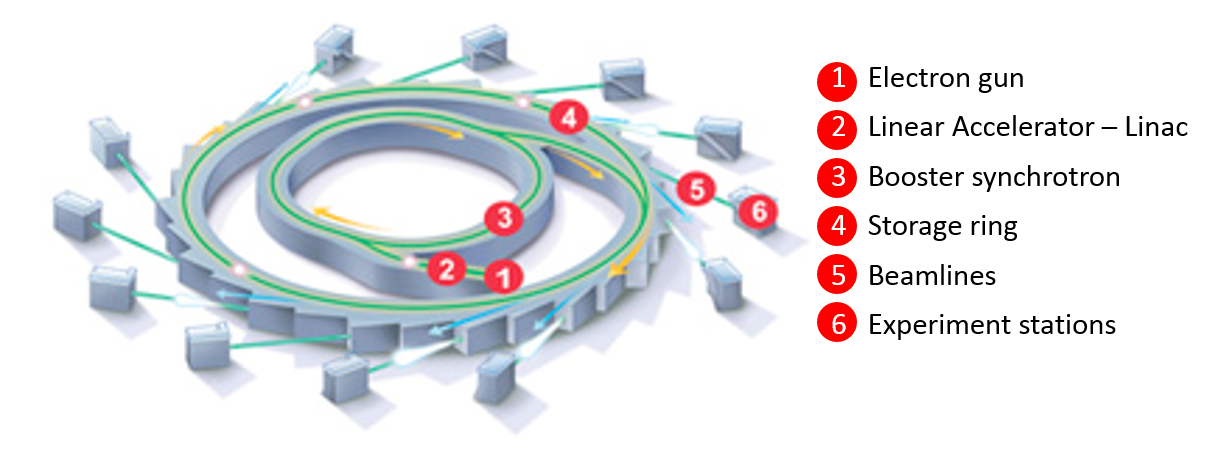
\includegraphics[width=\textwidth]{storage_ring_example.png}
        \caption[Schematic of a storage--ring--based light source.]{Schematic of a storage--ring--based light source showing the three main systems: the injection systems, composed of an electron gun, a \gls{linac} and a booster; the storage ring and the beamlines, with the experiment stations at their ends.}
        \label{fig:light_source_example}
    \end{figure}
    shows a generic scheme of a storage ring based light source. It has three main subsystems: an injector, the storage ring and the beamlines. The injector is responsible for generating and accelerating the particles up to the ultra--relativistic energy of the storage ring and in most light sources it is composed of a gun, a \gls{linac} and a booster synchrotron. In the case of electron storage rings the electron beam is emitted from cathodes in the gun, via thermoionic or photoelectric effect, and are compressed in bunches and accelerated by the \gls{linac}, generally up to energies of hundreds of \si{\mega\electronvolt}. After this, the electrons are transported to the booster synchrotron where they are accelerated up to the energy of the storage ring, generally a few \si{\giga\electronvolt}, and extracted from it to be injected into the storage ring. This whole process can happen with a repetition rate of a few \si{\hertz}.

    The storage ring is a synchrotron just like the booster in which the average energy of the electron beam is constant, while they perform dozens of billions of turns in the few hours they remain there. After injection, the bunches of electrons oscillate around the ideal orbit in the storage ring, but in a few dozens of thousands of turns they are damped, reaching the storage ring equilibrium values of transverse emittances (size and divergence), longitudinal length and energy spread. In ideal storage rings they stay stable in stationary closed orbits emitting radiation that is collected by the beamlines. The radiation exits the storage ring through holes in the external part of the vacuum chamber, called exit ports, and propagate to the beamline in straight trajectories, tangent to the electrons orbit in the point where it was generated.

\section{Storage Ring Main Devices} \label{sec:storage_ring_main_devices}

    This work will focus on the study of the dynamics of the particles while they are in their equilibrium regime inside the storage ring, without considering the details of the injection process. For this reason, in this subsection we will present the main subsystems of a storage ring and discuss their main contributions to the task of keeping particles in stable confinement for such long times. Throughout thes whole work the approximation $v\propto c$ will be assumed in the formulas, given the ultra--relativistic regime of the particles. Besides, all the equations are presented using the \gls{si}.

\subsection{Magnetic Lattice}

    Magnetic lattice is the series of static magnets that are placed along the beam trajectory to deflect and focus it to keep the motion stable. It is composed of a reduced number of distinct types of magnets that have specific functions for the beam confinement:
    \begin{description}[align=left]
        \item[Dipoles:] or bending magnets, are the devices responsible for deflecting the beam in such a way that its net deflection in one turn is \SI{2\pi}{\radian}. They generate an almost constant vertical field, $B_y$, along the beam path that curves its horizontal trajectory (see Figure~\ref{fig:dipole}).
        \begin{figure}
            \centering
            \begin{subfigure}[c]{0.45\textwidth}
                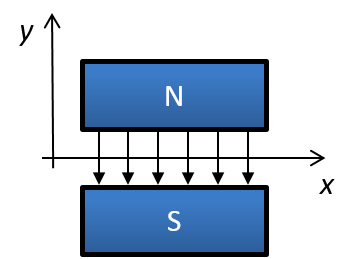
\includegraphics[width=\textwidth]{dipole_example.png}
                \caption{Schematic figure of a dipole magnet, where N and S indicate the North and South poles of the magnet and the vertical down arrows indicate the magnetic field lines}
            \end{subfigure}\hfill
            \begin{subfigure}[c]{0.5\textwidth}
                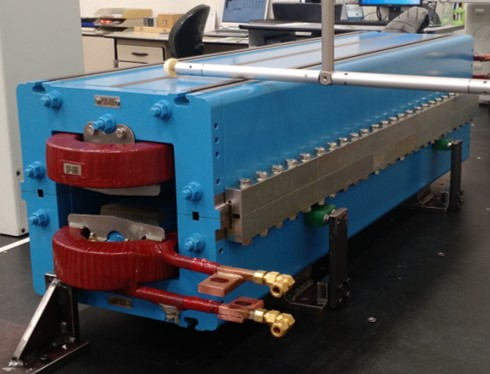
\includegraphics[width=\textwidth]{dipole_real.jpg}
                \caption{Picture of a real dipole magnet.}
            \end{subfigure}
            \caption{Illustrations of a dipole magnet.}
            \label{fig:dipole}
        \end{figure}
        At each point of the trajectory inside a dipole the curvature, $G(s)$, is given by:
        \begin{align}\label{eq:curvature_dipole}
            G(s) = \frac{1}{\rho(s)} = \frac{e}{p_0}B_y(s) \approx \frac{ec}{E_0}B_y(s)
        \end{align}
        where $s$ is the longitudinal position along the ring, $\rho(s)$ is the radius of curvature, $e$ is the absolute value of the particle's charge, $c$ is the speed of light, $p_0$ is the absolute value of the average linear momentum of the beam and $E_0$ is the corresponding average beam energy. Notice in the equation above that dipoles work as spectrometers, if the beam has an energy spread and in the absence of other types of magnets, particles with higher/lower energy will spiral out/in because their total deflection angle will be different than \SI{2\pi}{\radian}, which means eventually all particles will hit the vacuum chamber and be lost;
        \item[Quadrupoles:] are responsible to focus the beam, keeping oscillating around the ideal orbit. They achieve this by creating a field that grows linearly in intensity with the displacement from its center (see Figure~\ref{fig:quadrupole}),
        \begin{figure}
            \centering
            \begin{subfigure}[c]{0.47\textwidth}
                \centering
                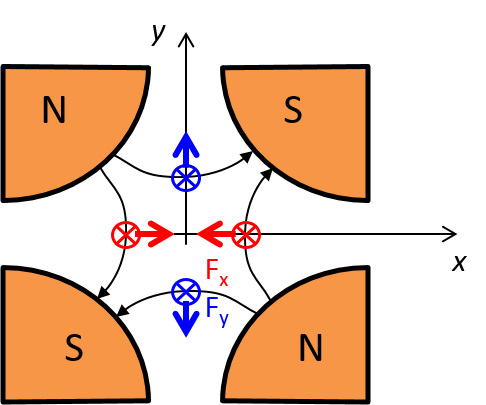
\includegraphics[width=0.55\textwidth]{quadrupole_example.png}
                \caption{Schematic figure of a quadrupole magnet, where the curved arrows indicate the magnetic field lines and the red/blue arrows indicate the direction of the horizontal/vertical forces felt by an electron entering the sheet. Notice this quadrupole focuses in the horizontal, so it is a focusing quadrupole.}
            \end{subfigure}\hfill
            \begin{subfigure}[c]{0.5\textwidth}
                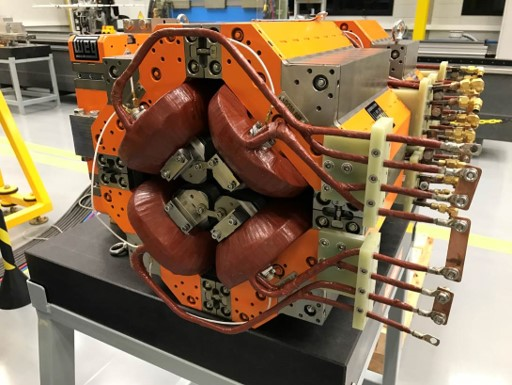
\includegraphics[width=\textwidth]{quadrupole_real.jpg}
                \caption{Picture of a real quadrupole magnet, with the coils that generate the magnetic field and the iron core that guide and shape the field lines inside the gap.}
            \end{subfigure}
            \caption{Illustrations of a quadrupole magnet.}
            \label{fig:quadrupole}
        \end{figure}
        in such a way that they work as lenses. They are characterized by their strength, defined by:
        \begin{align}
            K(s) = \frac{e}{p_0}\left.\derpar{B_y}{x}\right|_{y=0}(s)
        \end{align}
        where $x$ and $y$ are the horizontal and vertical displacement from the center of the quadrupole. The strength defined above is directly related to how much the quadrupole deflect off-centered particles, being its integral along the quadrupole length directly related to the focal length of the magnet. One intrinsic limitation of quadrupoles imposed by \gls{maxeq} and the Lorentz force is that they cannot focus the beam simultaneously in the horizontal and vertical directions. This means that two types of quadrupoles are needed in a magnetic lattice, one to focus in the horizontal, called focusing quadrupoles by convention, and another to focus in the vertical, the defocusing quadrupoles, in such a way that net focusing in both planes can be achieved with intelligent positioning of the magnets. Besides, quadrupoles are arranged along the ring to correct the intrinsic limitation of the dipoles regarding the energy dispersion, as discussed above, adding/subtracting net deflection in one turn for particles with more/less energy. This causes particles to have different closed orbits depending on their energy, the chromatic closed orbits. Quadrupoles and dipoles are the most important multipoles in a storage ring because together they define its main equilibrium properties, such as the particles average energy, the transverse beam natural emittance, and beam sizes along the ring, as well as the fundamental frequency of oscillation of the particles, the tune.
        \item[Sextupoles:] quadrupoles also suffer from chromatic aberrations, focusing more or less the particles depending on their energy. This difference in focusing makes particles oscillate differently around their closed orbit, changing their fundamental resonant frequency. This is not a conceptualy fundamental problem, but a practical one because in almost all modern storage rings it is impossible to store particles with only dipoles and quadrupoles. Sextupoles can correct that effect if placed at the right positions along the ring because of their non-linear magnetic field, which grows quadractically with the distance from its center, see Figure~\ref{fig:sextupole}.
        \begin{figure}
            \centering
            \begin{subfigure}[c]{0.47\textwidth}
                \centering
                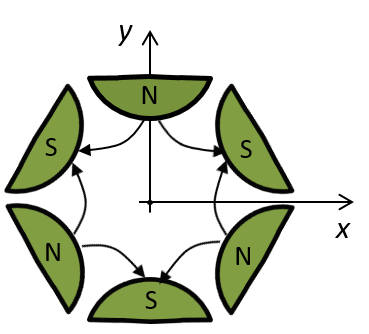
\includegraphics[width=0.9\textwidth]{sextupole_example.png}
                \caption{Schematic figure of a sextupole magnet, where N and S indicate the North and South poles of the magnet and the curved arrows indicate the magnetic field lines.}
            \end{subfigure}\hfill
            \begin{subfigure}[c]{0.5\textwidth}
                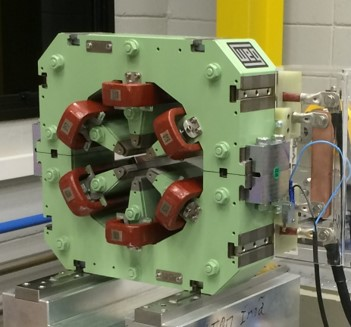
\includegraphics[width=\textwidth]{sextupole_real.jpg}
                \caption{Picture of a real sextupole magnet.}
            \end{subfigure}
            \caption{Illustrations of a sextupole magnet.}
            \label{fig:sextupole}
        \end{figure}
        Just like quadrupoles, it is needed two types of sextupoles, focusing and defocusing, to correct the horizontal and vertical frequency of oscillation of the particles. Sextupoles are needed, but they introduce several complications for the design of a storage ring, because their non-linear fields introduce chaos in some regions of the particles phase space. More sextupoles or higher order multipoles can be introduced to avoid chaos as much as possible and also to help correcting higher order chromatic effects.
    \end{description}

    Higher order multipole magnets, such as octupoles and decapoles, can be used to correct higher order chromatic and geometric aberrations, but their use is not very common in the design of storage ring for light sources as they are in colliders, even though this tendency is changing with the new light sources that are being designed, such as MAX IV~\cite{Leemann2009}, ESRF upgrade~\cite{Farvacque2013}, APS-U~\cite{Sun2013}, SLS upgrade~\cite{Soutome2016} and Spring-8 upgrade~\cite{Soutome2016}. Nevertheless, they are always present in storage rings as errors of the main magnets and their effect must be taken into account in detailed single particle dynamics analysis.

    Generally, lattices have high periodicity, being the repetition of a unit cell along the whole extension of the ring. This periodicity simplifies the design of the ring, the dynamics of the electrons and reduces the number of dangerous resonances that can harm the beam stability. Unit cells generally can be divided in two parts, an arc section, where the dipoles are placed, interleaved by focusing elements to control the dispersion and focus the beam from one dipole to another, and a straight section, with a dedicated space for the installation of \glspl{id} for light generation and other machine equipment. The straight sections also have focusing elements to match the beam to the arcs.

\subsection{RF Cavity}

    At each turn, the electrons lose energy due to synchrotron radiation which must be replenished periodically in order for them to remain in stable orbits, with energy close to the nominal energy of the storage ring. The magnetostatic components described above cannot perform such a task neither any other component or method relying on static electromagnetic fields of any kind, because according to the \gls{maxeq} and the Lorentz force, the net energy transfered to a charged particle by static fields in one turn over the ring must be zero. This means that the laws of physics constraint that it is necessary to rely on time dependent electromagnetic fields to replenish the energy of the electrons. The way this is accomplished in a storage ring is through the use of devices called RF cavities.

    The RF cavity is a cylindrical electromagnetic cavity with the lowest Transverse Magnetic mode (TM010) in the range of radiofrequency. Cavities for use in storage rings must have at least two small holes in its axis for the beam passage and one other hole to couple the cavity with an external source to feed the mode TM010 with energy. This energy is transfered to the particles when they pass through the cavity by the almost homogeneous longitudinal eletric field of this mode. The frequency of this particular mode is always exactly equal to a multiple, $h$, of the revolution frequency of the beam along the ring, in such a way that the phasing between the electric field and the beam entrance in the cavity remains constant over sereval passages and, once initially adjusted when the beam is injected in the ring, will be such that the average energy lost in one turn is replenished. This special phase is called the synchronous phase. Moreover, this synchronicity mechanism, that, by the way, is the responsible for the name of this type of accelerator, creates $h$ points in the ring's longitudinal phase space around which the electrons can form stable bunches.

    Besides the mode used to feed energy to the beam, a cavity can have several other modes of higher resonant frequencies with a high quality factor, $Q$, that can be excited by the beam. When the beam passes through the cavity it leaves electromagnetic fields with a very wide spectrum of frequencies. Most of these frequency components are rapidly scattered and dissipated, but some of them, close to the resonant frequency of these modes, can last for very long times and, assuming the beam is constantly feeding them, strong electric potentials, or wake fields, can be formed. These potentials, in turn, influence the beam dynamics, causing energy loss, distortion of the bunches and instabilities.

    There are some methods to avoid this problem with cavities. For example, it is possible to insert couplers in the cavity, similar to the one that feeds the fundamental mode, but designed and positioned specially to interact with one or a group of these \glspl{hom} to absorb the energy deposited by the beam, which is later transformed in thermal energy by resistors outside the cavity, or to design wave guides in the cavity, through which the modes can propagate and be dissipated in the resistive endings. Another method involves shifting the frequency of the modes, via thermal or mechanical deformation, in such a way that they do not couple with any frequency of the beam.

    The superconducting RF cavities also do not have this problem because they are built with very large tubes for the beam passage, in such a way that the \glspl{hom} can propagate through them. Even though for the main mode the ratio of the shunt impedance by the quality factor, $R_s/Q$, which depends only on the geometry of the cavity, as explained by~\citeonline[Sec. 15.4]{Wiedemann2007}, is strongly reduced by this approach, the zero resistivity of the wall still provides very large values for $Q$ and $R_s$. Sirius will adopt this type of cavity and, based on the operation reports of other laboratories which also employed this solution, we do not expect to have problems with \glspl{hom}.

\subsection{Vacuum System}

    The vacuum system is used to create a compact region around the reference orbit in the whole machine with very low pressure, and thus minimize collisions of the stored charged particles with residual gas molecules, increasing the lifetime, which is the average time particles can be stored with stable movement, and minimizing the production of bremstrahlung radiation. As an estimative, the average pressure of a storage ring must be lower than \SI{1}{\nano Torr} for the average stored time of the particles to be of the order of a few dozens of hours.

    The vacuum system is composed of two main subsystems, the vacuum vessel, which defines the boundaries of the electron's environment, and vacuum pumps, which maintain the desired difference in pressure between the two regions. Most of the extension of the vacuum vessel is composed of straight and long chambers with a specific cross section, constant along the extension of the chamber. They are made of metals due to several desirable properties of these materials, such as high heat and electrical conductivities, high acceptance to welding and brasing, high resistance to pressure and low cost. Among them we highlight implications of the high electrical conductivity, due to its importance for this work. Besides the standard vacuum chamber there are several other structures that compose the vacuum vessel, for example:
    \begin{description}[align=left]
        \item[Bellows:] are sanfonated elements that connect two vacuum chambers in order to accommodate longitudinal thermal expansions and transverse misalignments between them, as well as the assembly to the vacuum components themselves;
        \item[Valves:] devices that are used to isolate the vacuum in different sections of the ring. Generally they remain open, creating a single vacuum region along the ring, but can be closed automatically in case of accidents, or for maintenance;
        \item[Flanges:] are the components responsible for coupling two different vacuum components together in a leakage-free manner;
        \item[Dipole Chambers:] are special curved chambers used in the regions where there are dipoles. In some cases they have exit ports to extract the photon beam to the beamlines;
        \item[Radiation Masks:] are small protuberances in the vacuum chamber designed to shadow more sensitive elements from synchrotron radiation.
        \item[Diagnostic Elements:] are components used both to measure the electromagnetic signals generated by the beam to determine its properties, such as intensity, position and oscillations and act back on it either as a feedback or feedforward corrections to perturbations. They must be inside the chamber because the high frequency components they measure cannot propagate out the chamber;
        \item[Transitions:] there are some sections of the vessel that have different cross sections than the standard chamber, generally to accomodate special devices such as RF cavity, \glspl{id}, some magnets, ceramic chambers, collimators, etc. Transitions are smooth longitudinal variations of cross section from one chamber to the other.
    \end{description}

    These are only some examples of the different components of the vacuum vessel of a storage ring. All these components introduce variations in the inner cross sections of the chamber which interact with the electromagnetic fields of the beam, creating other fields, called wake fields, that causes not only heating of the components, in addition to the radiation heating, but also act back on the beam itself affecting its dynamics with the potential of causing instabilities that can severely limit the machine performance. The study of this last interaction applied to the new Sirius light source in Brazil will be the main subject of this work.

\section{Light Source Generations}

    Brightness is the main figure of merit used to characterize a synchrotron light source~\cite{Hettel2014a}, the larger its value the better the radiation. It is a measure of the intensity and collimation of the radiation at a given frequency or wavelength and can be mathematically defined by the following expression, according to \citeonline{Huang2013}:
    \begin{align}\label{eq:brightness}
        B(\omega) = \frac{1}{\Delta\omega}\frac{F(\omega)}{\Sigma_x(\omega)\Sigma_y(\omega)}
    \end{align}
    where $\omega$ is the photon frequency, $F(\omega)$ is the flux, the average number of photons per second, $\Sigma_x$ and $\Sigma_y$ correspond to the volume the photon beam occupies in the horizontal and vertical phase space, respectively, and $\Delta\omega$ is a frequency bandwidth that is proportional to the central frequency (usually \SI{0.1}{\percent}). The volume occupied by the photon beam in phase space is convolution of the electron beam distribution and the photon distribution emitted by a single electron. This last term depends on the radiation frequency and on how it was generated. On the other side, the volume occupied by the electron beam in phase space is called emittance and it depends only on the storage ring properties.

    Equation~\eqref{eq:brightness} shows that to increase the brightness of a given light source it is necessary to increase the number of stored electrons, which linearly impacts the total photon flux, and minimize the emittance of the electron beam. Consequently, together with the electrons energy, the emittance and the current are the main figures of merit of a storage ring. New machines always try to push the limit of these factors to obtain gains in synchrotron light quality and, from time to time, new ideas and breakthroughs in accelerator technology create large scale advances.

    These discontinuities in the otherwise small and incremental improvements of the radiation quality happened three times along the history of storage ring based light sources, classified as four generations of machines. The first breakthrough was the construction of machines dedicated to the generation of synchrotron radiation from dipoles, which marked the difference from the first generation of light sources, which were parasitical to particle colliders.

    The second breakthrough was the construction of machines specialized to operate with \glspl{id}, which are special devices that are installed along the straight trajectory of the beam and generate a transverse magnetic field with an amplitude that varies sinusoidally along the longitudinal direction. When the beam passes through this field it wiggles, and synchrotron emission of radiation happens due to its deflection at each wiggle. The light emitted from successive wiggles interferes in such a way that only photons with specific frequencies survive and the resulting radiation has a spectrum where all the energy is concentrated at very thin peaks around multiples of this resonant frequency. The intensity of these peaks is proportional to the number of particles in the beam and the number of wiggles of the \gls{id} field and their bandwidth is proportional to the inverse of the number of wiggles. Additionally, the polarization of the radiation is defined by the direction of the magnetic field of the \gls{id}. For example, if the field is vertical, the electrons will oscillate horizontally and the radiation will be horizontally polarized. In specially designed \glspl{id}, circular and elliptical polarizations can also be achieved by changing not only the intensity of the field but also its direction as a function of the longitudinal position. All these properties of the light can be tuned according to the needs of the experiment to be carried out at the experimental station, which makes these devices a very powerful tool for scientific investigations.

    Currently, another generation of light sources is rising. With much smaller emittances, these machines are being called \gls{4gls}.
    % This term is used when the emittance of the electrons is smaller than the emittance of the single photon distribution up to a few \si{\kilo\electronvolt}. This way, the convolution of the two is mainly determined by the method the radiation is generated, which in turn is defined by the laws of nature and cannot be further optimized.
    This search for smaller emittance becomes clear when we observe the graph shown in Figure~\ref{fig:scaled_emittances}
    \begin{figure}
        \center
        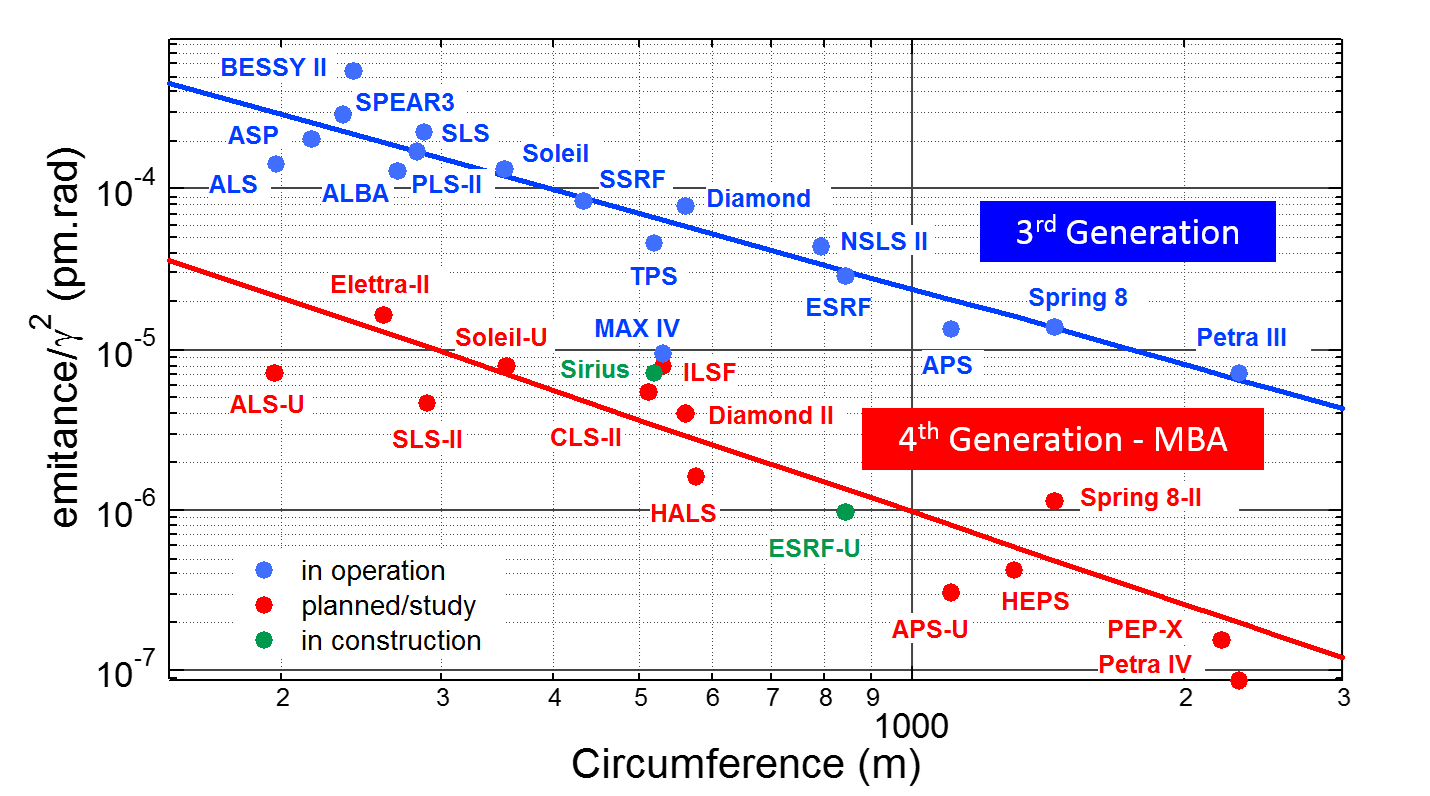
\includegraphics[width=\textwidth]{emittance_third_versus_fourth.png}
        \caption[Comparison of machines emittances.]{Natural emittance normalized by relativistic energy squared as function of ring circumference for several existing \gls{3gls} and future \gls{4gls}. The blue solid line is a fitting among the \gls{3gls} and the red solid line is a fitting among the \gls{4gls}. Note the only \gls{4gls} in operation today is MAX-IV. Updated from~\cite{Liu2017}.}
        \label{fig:scaled_emittances}
    \end{figure}
    which compares the 3$^\text{rd}$ and \gls{4gls}. To interpret this figure it is important to know that the emittance of a storage ring roughly scales with
    \begin{align}
        \varepsilon \propto \frac{\gamma^2}{N_b^3},
    \end{align}
    where $\gamma = E/m_0c^2$ is the relativistic energy and $N_b$ is the number of dipoles, or bending magnets, of the storage ring. Besides, higher energy storage rings generally imply in larger circumferences and, consequently more dipoles. Given the scaling presented above, it is clear that in general the emittance is reduced with the increase of the ring circumference, as shown by the tendency lines in the figure.

    The \gls{4gls} will enable new science to be made, according to~\citeonline{Eriksson2014}:"The significant improvement provided by the DLSRs (Diffraction Limited Light Sources, or \gls{4gls}) under construction and in the design stage will enlighten our view of the world and allow science which is not possible, or not even thinkable, today.". In section 4 of his article,~\citeauthor{Eriksson2014} provides a very good review of the possible scientific studies that will be enabled by such machines. Here we highlight the advances in imaging techniques, such as ptychography~\cite{Thibault2014}, and diffraction~\cite{Hitchcock2014}, that will be possible due to the increase in the transverse coherent part of the flux~\footnote{For a brief and didactic description of coherence, we recommend the work of~\citeonline{Huang2013}.}.

\subsection{\Glsentryfull{mba}}

    The main reason for the \gls{4gls} to achieve such small emittances is the use of \gls{mba} lattices. In \gls{3gls} the number of dipoles in one unit cell of the magnetic lattice is two or three depending on the machine, but in \gls{4gls} this number is larger than five, hence the name multi-bend. The achromat part of the name \gls{mba} is due to the fact that energy dispersion errors introduced by dipoles are corrected locally and do not affect the trajectories and transverse bunch sizes inside the \glspl{id}.

    Even though this change does not seem to be harmful or difficult in a first analysis, it requires several developments in almost all the areas involved in designing, constructing and operating a light source~\cite{Eriksson2014,Liu2017}. The larger number of dipoles in a short space requires strong focusing from the quadrupoles to achieve low emittances. These strong quadrupoles require strong sextupoles to correct their chromatic errors, which, in turn, require other strong sextupoles to increase the stability region around the fixed point of the one--turn map~\cite{Borland2014}. In order to produce all these strong magnets, they need to be closer to the beam, their gap must be smaller~\cite{Johansson2014}, which implies the vacuum chambers must be smaller too. The smaller vacuum chamber decreases the vacuum conductance\footnote{The vacuum conductance is proportional to the third power of the vacuum chamber radius, as described by~\citeonline{Al-Dmour2014}.}, making it necessary to adopt different solutions for vacuum pumping~\cite{Al-Dmour2014}, generally distributed along the whole ring, such as the use of \gls{neg} coating inside the chambers, first proposed by \citeonline{Benvenuti1983}.
    The proximity of the vacuum chamber and all the other in--vacuum components to the beam, increase the beam coupling impedance, which leads to higher heating of the components and to instabilities~\cite{Nagaoka2014}. The stronger magnets also imply more sensitivity of the lattice to errors, such as construction errors of the magnets, misaligments and residual multipoles~\cite{Neuenschwander2015,Hettel2014}, and, together with the very small transverse sizes of the beam, require tight tolerances power supply stability and vibration, not only of the magnets and \glspl{bpm}, but also of the components of the beamlines, such as the monochromators~\cite{Susini2014,Siewert2014} and also for the detectors at the experimental stations~\cite{Denes2014}. Underlying all these intrincacies is the need of very detailed design, characterization and, in some cases measurement, of all the components that are installed in the light source. Besides, detailed single particle models of the storage ring are fundamental to evaluate the effect of each new design on the global properties of the ring, such as beam lifetime and dynamic aperture. All this requires very detailed simulations and high computational power~\cite{Borland2014}.

    Regarding the beam coupling impedance, the last \gls{3gls} that were built already demonstrated a need to evaluate the budget of the ring, simulating and, more importantly, designing the components to minimize heating and other impedance related issues~\cite{Nagaoka2004a,Gunzel2008,Blednykh2007,Blednykh2009}. For \gls{4gls} this approach is practically mandatory because the predictions for thresholds for strong instabilities are much lower for these machines than they were for \gls{3gls}~\cite{Klein2013a,Lindberg2015,Persichelli2017a,Wang2017,Wang2017a}.
    Additionally, the use of~\gls{neg} technology extended along the whole ring requires more detailed analysis of its effect on the impedance.

\section{Collective Effects}

    Collective effects can cause severe deterioration of the brightness of a machine because they can lead to the increase of the effective emittance of the electron beam, through coherent oscillations of the bunches, increase of the energy spread and the beam sizes in all three planes. Besides, they can cause beam loss, which limits the maximum current that can be stored and consequently the total photon flux of the machine. In this section we will introduce the main mechanisms that drive collective effects in a storage ring.

\subsection{Interaction Mechanisms}

    One of the most important interaction in storage ring light sources is the collision of particles in the beam, generally refered to as Coulomb scattering or \gls{ibs}, which is highly chaotic and its effects on the beam resembles the properties of the emission of radiation, causing emittance and energy spread increase~\cite{Piwinski1974,Bjorken1983,Kubo2001}. Additionally, the collision process also leads to particle loss through a mechanism called Touscheck scattering, first explained by Bruno Touschek~\cite{Bernardini1963}, described in details by \citeonline{Piwinski1999}, where the transverse energy of oscillation is transfered to the longitudinal plane and the particles gain/lose an energy deviation so large that they are lost. All these effects are very detrimental to new light sources, being the Touscheck lifetime their main source of particle loss, as pointed out by \citeonline{Nagaoka2014}.

    The \gls{dsp} is another type of interaction among the particles, being the result of the action of the cloud of electromagnetic field existent inside the beam on individual particles. Each particle generates an electric and a magnetic field that, when averaged among all particles, result in a net potential dependent on the shape and sizes of the bunch. This potential acts like an external field on the movement of the particles, leading to tune--shifts with amplitude and possible excitation of resonances. However, for ultra-relativistic electron beams such as the ones of a light source storage ring, with energies on the order of a few \si{\giga\electronvolt}, this effect is very small and can be neglected. This happens because in this limit the non-radiating field generated by each particle is concentrated in a plane transverse to its movement and the electric and magnetic forces that act on other particles moving parallel to it cancel each other out. In Appendix~\ref{app:lorentz_cancel} a more detailed explanation for this property is given.

    The \Glsentryfull{csr} is another type of direct interaction between particles in a beam. The radiation emitted by the particles travels forward with the velocity of light and, due to the fact that the particles are moving on a curved trajectory when they emit light, this radiation catches up with the particles ahead of the emitting particle~\cite{Derbenev1995}. If the wavelength of the radiation is of the same order of or larger than the bunch length, the average of this effect is non-zero and the head of the bunch feels a net force. As this effect depends on the radiated field, in contrast to the \gls{dsp}, it does not tend to zero as the energy on the particles increases and can be very harmful, depending on the bunch length of the beam, causing energy spread increase and bunch lengthening or even microbunching~\cite{Byrd2002}.

    All mechanisms described above are examples of direct interactions among the particles, they do not depend on the immersive environment to happen. The wake fields and the \gls{isp} on the other hand, results from the interaction with the vacuum chamber. The contact of the non-radiating field of the beam with the metallic walls of the chamber induces currents in the surface of the metal that travels with the beam, these surface currents also generate an electromagnetic field that propagates to the center of the vacuum chamber and influences the movement of the particles, as described by \citeonline{Laslett1963}. This electromagnetic field can have properties of non-radiating and radiating field, depending on the characteristics of the vacuum chamber. If we consider the chamber is perfectly conducting and with translational symmetry in the longitudinal direction, then the surface charges travel in straight lines with the beam speed, which means they will produce only non-radiating fields with the same properties of those of the \gls{dsp}. This is the origin of the \gls{isp}, that for the same reasons as the \gls{dsp} is negligible for high energy storage rings\footnote{This statement is not true for static (or quasi--static) fields, because the electric and magnetic components of the force decouples and they depend on whether or not the boundary is a good electric conductor or a high--$\mu$ magnetic material. This problem was first studied by \citeonline{Laslett1963} and will be addressed later in this work.}.

\subsection{Wake Fields}\label{ssec:wake_fields}

    If any of the two conditions considered for the vacuum chamber does not hold, then the surface charges also generate radiating fields or fields that are dragged behind the source particle, namely wake fields. For example, if the vacuum chamber has no longitudinal translational symmetry, then the surface charges must follow curved paths, which makes them suffer accelerations and hence, radiate electromagnetic fields. Notice that this is only one of the several possible ways of introducing this mechanism, it would be equivalent to say that the surface of the metal scatter the fields generated by the particles in the beam and when the surface of the vacuum chamber has longitudinal symmetry the reflection is specular but when it has corrugations or transitions, the scattering is diffuse. Precisely what happens is that the walls of the vacuum chamber impose boundary conditions on the fields that exist inside the vacuum vessel, univocally defining its time and spatial dependency.

    The wake fields can be very harmful to the beam, changing the properties of the static distribution of particles and creating instabilities above a given current threshold, which can lead to coherent oscillations of the bunches, emittance and energy spread increase and even beam loss. All these effects cause serious deteriorations of the brightness of the radiation, limiting the photon flux and bringing deterioration of its phase space average distribution.

\section{The Sirius Project}

  	The \gls{cnpem} is a Brazilian institution located in Campinas-SP that gathers four national laboratories, being the \gls{lnls} one of them. This laboratory was created in 1987 to design, construct and operate a \gls{sls}. Such goals were successfully achieved with UVX, a second generation light source that was openned to external users in 1997. Since them, the Brazilian community of synchrotron users has grown and studies of a new, more competitive machine, started in 2008.

    By the end of 2011, Sirius was a well--developed project and it consisted on a permanent magnet--based \gls{3gls}, with an energy of \SI{3}{\giga\electronvolt}, an emittance of the order of \SI{2}{\nano\meter\radian} and circumference of \SI{480}{\meter}, as described by~\citeonline{Liu2010} and \citeonline{Liu2011}. This scenario changed after the first meeting of the \gls{mac}, in June 2012, when the committee recommended leaders to follow the idea of MAX-IV~\cite{Leemann2009} and pursue sub-nanometer emmittances. This challenge was accepted and Sirius became the second project to fit the category of what today is called \gls{4gls}, with a natural emittance even lower than the first projected machine of this kind, the MAX-IV~\cite{Liu2013}.

    After several changes in the magnetic lattice~\cite{Liu2014,Liu2015,Liu2016} to improve the brightness of the light generated by the \glspl{id} that are being planned for Sirius~\cite{Sirius2013,Vilela2017}, the current lattice of the storage ring is the one presented in Figure~\ref{fig:sirius_lattice}
    \begin{figure}
        \centering
        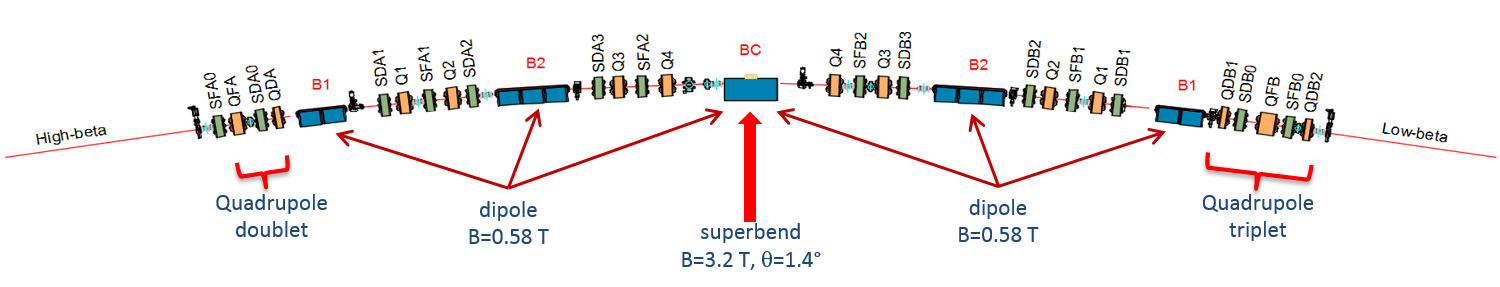
\includegraphics[width=\textwidth]{sirius_lattice.png}
        \caption[One fourth of the unit cell of the Sirius storage ring.]{One fourth of the unit cell of the Sirius storage ring. Dipoles are shown in blue, quadrupoles in orange and sextupoles in green. The vacuum pumps and valves are also shown. Only half of the high-beta (A) and of the low-beta (B) straight sections are shown. The arc and the straight sections are repeated to form the unit cell in the following way: A-B-B-B. The unit cell is then, repeated five times to form the ring.}
        \label{fig:sirius_lattice}
    \end{figure}
    and the current optical functions are presented in Figure~\ref{fig:sirius_twiss}.
    \begin{figure}
        \centering
        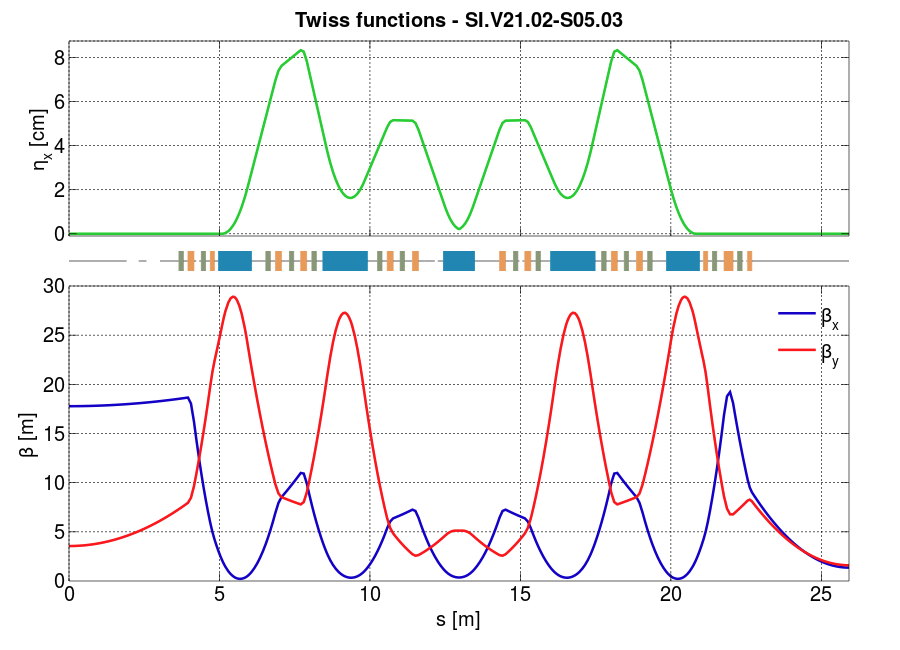
\includegraphics[width=\textwidth]{SI_twiss.png}
        \caption[Twiss functions of the Sirius storage ring.]{Optical (twiss) functions for one fourth of a period of the Sirius lattice. In green is shown the dispersion function. In red, the vertical betatron function is shown and in blue, the horizontal betatron function. Notice the strong focusing of the betatron functions at the center of the low-beta (B) sections. (copied from \citeonline{Sirius2013}.)}
        \label{fig:sirius_twiss}
    \end{figure}
    The arc of the cell, composed of all the elements from the first to the second B1 dipoles, inclusive, is repeated twenty times to form the ring. The straight sections alternate in sections with two quadrupoles in each matching extremity (A), and sections with three quadrupoles (B), in the following manner: A-B-B-B, in such a way that the ring has five A sections and fifteen B sections. The difference between these two types of sections is that beam is strongly focused in both directions, horizontal and vertical, in the B sections, to improve the radiation generated by the undulators which will be installed there and the A sections are optimized for off--axis injection in the horizontal plane. This way the ring has twenty straight sections, from which eighteen will be available for installation of \glspl{id}. However the real symmetry of the ring is only five, which difficults the optimization of the single particle non-linear optics~\cite{Sa2016, Dester2017}. In the center of each arc there is a special dipole magnet, with longitudinal gradient and a strong peak field of \SI{3.2}{\tesla} in its center that will provide hard x-rays, with critical energy of \SI{19.2}{\kilo\electronvolt}, for additional 20 beamlines~\cite{Liu2016,Sirius2013}.

    The whole accelerator complex of the Sirius \gls{sls}, shown schematically in Figure~\ref{fig:accelerator_complex},
    \begin{figure}
        \centering
        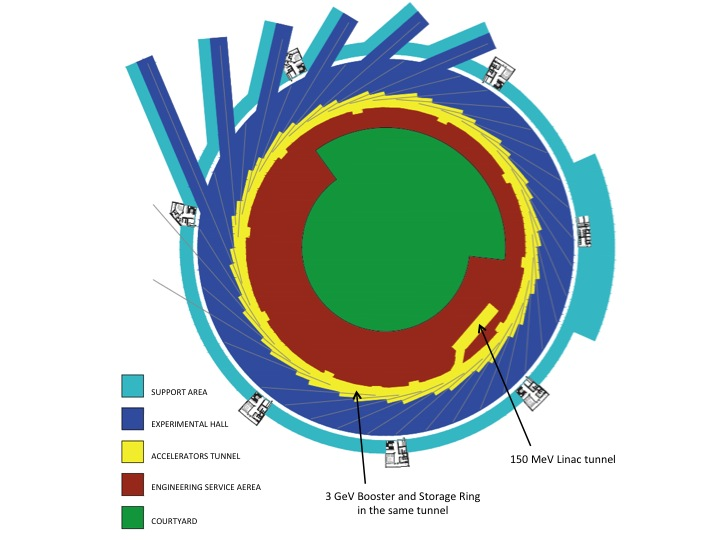
\includegraphics[width=0.9\textwidth]{Sirius_building_layout.jpg}
        \caption[Sirius building layout.]{Sirius building layout, showing all the important areas of the light source, with emphasis on the booster sharing the same tunnel as the storage ring and the \SI{150}{\mega\electronvolt} \gls{linac} tunnel. The experimental hall will be able to accomodate beamlines up to \SI{100}{\meter} long and the requirement for longer beamlines, with possible length up to \SI{450}{\meter}, is anticipated. (copied from \citeonline{Sirius2013}.)}
        \label{fig:accelerator_complex}
    \end{figure}
    will be composed of a \SI{150}{\mega\electronvolt} \gls{linac}, a full energy booster synchrotron, that will ramp the electrons from the \gls{linac} energy to the storage ring nominal energy with a cycling rate of \SI{2}{\hertz}, and the storage ring, as described in ~\citeonline{Sirius2013} web page. The injection system will operate in top--up mode, where the total current of the storage ring is kept nearly constant during the whole user's shift, because periodic injection cycles along the day are performed without the need of interrupting the operation of the machine. The booster will be concentric to the storage ring and placed inside the same tunnel, which minimizes costs related to the construction of a separate shielding and helps diminishing its emittance, only \SI{3.5}{\nano\meter\radian} at \SI{3}{\giga\electronvolt}~\cite{Sa2014a}, which is important to maximize the injection efficiency in the storage ring~\cite{Liu2016a}.

    Table~\ref{tab:sirius_main_parameters}
    \begin{table}
        \centering
        \caption{Main Parameters of the Sirius Storage Ring.}
        \label{tab:sirius_main_parameters}
        \begin{tabular}{lccccl}
            \mr{2}{*}{Parameter} &  \mr{2}{*}{Symbol} & \mc{3}{c}{Operation Phases}& \mr{2}{*}{Unit}\\\cline{3-5}
                                 &                    &Commiss. & Phase 1 & Phase 2& \\\toprule
            Energy               & $E_0$     & \mc{3}{c}{3.0}    & \si{\giga\electronvolt}\\
            Circumference        & $L_0$     & \mc{3}{c}{518.4}  & \si{\meter}\\
            Revolution period    & $T_0$     & \mc{3}{c}{1.73}   & \si{\micro\second}\\
            Revolution frequency & $f_0$     & \mc{3}{c}{578}    & \si{\kilo\hertz}\\
            Angular rev. freq.   & $\omega_0$& \mc{3}{c}{3.632}  & \si{\mega\radian\per\second}\\
            Harmonic number      & $h$       & \mc{3}{c}{864}    & \\
            Momentum compaction  & $\alpha$  & \mc{3}{c}{\SI{1.7e-4}{}}& \\
            Transverse tunes (H/V)& $\nu_{x/y}$   & \mc{3}{c}{49.11/14.17}  & \\
            Energy loss per turn & $U_0$     & \mc{3}{c}{473}    & \si{\kilo\electronvolt} \\
            Natural emittance    & $\varepsilon_0$& \mc{3}{c}{252}& \si{\pico\meter\radian} \\
            Natural energy spread& $\sigma_\delta$& \mc{3}{c}{\SI{8.5e-4}}& \\
            Damping times (H/V/L)& $\tau_{x/y/z}$ & \mc{3}{c}{16.9/22.0/12.9}& \si{\milli\second}\\
            Damping rates (H/V/L)& $\alpha_{x/y/z}$ & \mc{3}{c}{59.2/45.5/77.5}& \si{\hertz}\\\midrule
            Nominal total current& $I_0$     & 30    &  100  & 350 & \si{\milli\ampere}\\
            Current per bunch    & $I_b$     & 34.7  &  116  & 405 & \si{\micro\ampere}\\
            RF cavity            &  & 1 7-Cell & \mc{2}{c}{2 SC-RF}  \\
            Voltage gap          & $V_0$     & 1.8   & \mc{2}{c}{3.0}& \si{\mega\volt} \\
            Natural bunch length & $\sigma_z$& 3.2(10.7) & \mc{2}{c}{2.5(8.2)}& \si{\milli\meter} (\si{\pico\second}) \\
            Synchrotron Tune     & $\nu_z$& \SI{3.56e-3} & \mc{2}{c}{\SI{4.6e-3}}& \\\bottomrule
        \end{tabular}
    \end{table}
    shows the main global parameters of the storage ring for the planned operation phases of the machine. Even though the commissioning will be performed with a normal conducting PETRA 7-Cell RF cavity, in the users operation phases of the storage ring the RF cavities will be \gls{supcond}. The installation of a 3th harmonic passive landau cavity to lengthen the bunches and increase the lifetime is foreseen, allowing multi-bunch operation with higher currents. Even though the expected filling pattern of the machine is uniform, other arbitrary filling patterns are possible and, in particular, gaps may be needed to cure ion instabilities~\cite{Wang2013a,Nagaoka2014}.


%%%%%%%%%%%%%%%%%%%%%%%%%%%%%%%%%%%%%%%%%%%%%%%%%%%%%%%%%%%%%%%%%%%%%
%%%%%%%%%%%%%%%%%%%%%%%%%%%%%%%%%%%%%%%%%%%%%%%%%%%%%%%%%%%%%%%%%%%%%
\chapter{Single--Particle Dynamics}\label{cap:single_particle_dynamics}

    In this chapter the main concepts of single particle dynamics that will be useful for the rest of the work will be introduced without any intention to be complete or rigorous in the presentation. There are good books, for example the ones written by~\citeonline{Lee1999} and by~\citeonline{Wiedemann2007}, and also one outstanding report written by~\citeonline{Sands1970} that cover all the topics presented here and much more, with thoughtful didactics. Besides, \citeonline{Borland2014} give a quick overview on all the topics relevant for single particle dynamics.

\section{Reference System}

    Connected to the concept of a storage ring is the one of the reference orbit. This special closed orbit is the one that an ideal particle, the synchronous particle, with the storage ring nominal energy would follow if it had the correct initial conditions. All the components of a storage ring are aligned according to this special orbit in such a way that their center, symmetry points or axis coincide with it and, in practice, the trajectories of all particles stored in the machine will be close to it. For this reason, the reference orbit is chosen to be the origin of the reference frame, defining a curved coordinate system that moves along the ring, with one longitudinal coordinate tangent to the local orbit and two transverse coordinates perpendicular to it. This type of co-moving coordinate system is a particular case of a Frenet-Serret frame~\cite{Frenet1852,Serret1851,wiki2017}, where the torsion is always zero, since storage rings are usually designed only with dipoles that deflect in the horizontal plane. Such a coordinate system can be defined in the following way~\cite[chap. 2]{Lee1999}:
    \begin{align}\nonumber
        \versor{s}(s) &= \dertot{\vect{r}_0(s)}{s},\\
        \versor{x}(s) &= -\rho(s)\dertot{\versor{s}(s)}{s},\\\nonumber
        \versor{y}(s) &= \versor{s}(s) \times \versor{x}(s),
    \end{align}
    where $s$ is the arc length of the reference orbit starting from an arbitrary point, $\vect{r}_0$ is the position of the reference orbit in relation to a static, cartesian reference frame, $\versor{s}$ is the Frenet--Serret vector tangent to the orbit, $\versor{x}$ is the negative of the normal vector, generally known in accelerator physics literature as radial or horizontal coordinate, $\versor{y}$ is the standard binormal versor, often called vertical direction in accelerator physics. The scalar $\rho$ is the local radius of curvature of the reference orbit, which is equal to the one introduced by the dipoles, as defined in equation~\eqref{eq:curvature_dipole}. This means that the reference frame of an accelerator is piecewise straight with curvature different from zero only at the dipole field regions.

    With the definitions above, the position of an arbitrary particle can be described as small deviations from the reference orbit (see Figure~\ref{fig:reference_frame})
    \begin{align}
        \vect{r}(s) = \vect{r}_0(s) + x\versor{x}(s) + y\versor{y}(s)
    \end{align}
    \begin{figure}
        \centering
        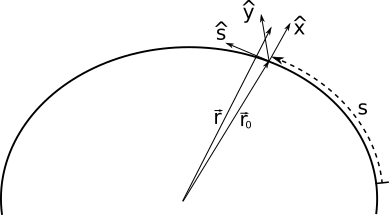
\includegraphics[width=0.65\textwidth]{coordinate_system.png}
        \caption[Frenet-Serret reference frame of a storage ring]{Frenet-Serret reference frame of a storage ring, with right-handed coordinate system $\{ \versor{x}, \versor{y}, \versor{s} \}$. Adapted from~\cite[pp. 123]{Lee1999}.}
        \label{fig:reference_frame}
    \end{figure}
    with $x$ and $y$ being the horizontal and vertical displacements of the particles in relation to the reference orbit. In this reference frame, the dynamics of each particle can be represented by its position in the six dimensional phase space defined by:
    \begin{align}\label{eq:phase_space_definition}
        \left\{ x, x', y, y', z, \delta \right\}
    \end{align}
    with
    \begin{align}
        x' = \dertot{x}{s} \approx \frac{p_x}{p},\quad
        y' = \dertot{y}{s} \approx \frac{p_y}{p},\quad
        \delta = \frac{p}{p_0}-1
    \end{align}
    where $p_0$ is the storage ring nominal linear momentum, $\delta \approx \Delta E/E_0$ is the energy deviation of the particle in relation to the nominal energy of the storage ring and $x'$ and $y'$ are the normalized transverse components of the linear momentum of the particle. The coordinate $z$ is defined as the relative longitudinal position of the particle in relation to the synchronous particle
    \begin{align}\label{eq:longitudinal_deviations}
        z(t) \coloneqq s_\text{sync}(t) - s(t)
    \end{align}
    where $t$ is the wall-clock time and $s_\text{sync}(t)$ is the trajectory arc-length of the synchronous particle. Note that if the particle is ahead of the synchronous particle $z$ will be negative. This convention is very important and will be consistently adopted throughout this work.

\section{Transverse Dynamics}

    At this point it is convenient to describe in general terms the movement of the stored particles in storage rings similar to Sirius'. The particles are ultra--relativistic electrons with energy of the order of a few \si{GeV}, and most of their velocity is always locally tangent to the ideal orbit. There are typically hundreds of billions electrons grouped in several bunches along the reference orbit, each bunch having length of a few milimiters and transverse sizes of the order of dozens of microns. Each electron is under the influence of a variaty of electromagnetic fields (gravity can be neglected), coming from the static magnetic fields of the dipoles and multipoles, the radiofrequency field of the RF cavity, the direct fields of other electrons in the same bunch and the fields scattered by the vacuum vessel, generated by other electrons in the same bunch, in other bunches or even by themselves in previous turns. Also, they emit synchrotron radiation in a random manner, which makes them lose energy and perturbs their movement with a recoil effect.

    The description of the dynamics of the stored particles begin with an approximation that neglects the effects of their self--generated fields, i.e. their interaction with each other, with the vacuum chamber and with the residual molecules in their atmosphere. In this framework the only forces acting on the particles are the magnetic fields of the dipoles and multipoles and the longitudinal electric field of the RF Cavity and the only way they can lose energy is through synchrotron radiation emission. Under such conditions, the one--turn map of the ring defines a fixed point in the phase space defined in equation~\eqref{eq:phase_space_definition} and the particles oscillate around it, being the oscillations in the planes $\{x,x'\}$, $\{y,y'\}$ and $\{z,\delta\}$ practically uncoupled. The oscillations in the first two planes are called transverse oscillations, while the one in the third plane is denominated longidutinal oscillation.

    For current synchrotrons, the dynamics of the longitudinal motion is much slower than the dynamics of the transverse motion. As an example, in the Sirius storage ring particles take approximately 215 revolutions around the ring to complete one turn around the fixed point in the longitudinal direction while they oscillate 49 times per revolution around the fixed point in the transverse plane. This property makes it possible to separate the study of the longitudinal plane from the transverse one, considering the energy deviation of one particle as a constant parameter in the transverse equations of motion. The effects of the radiation energy loss are even slower than the longidudinal motion, taking a few thousands of turns in the ring to significantly change the transverse motion.

    Neglecting the energy variations of the particles, and the randomnes of the radiation emission, the motion of the particles can be described by a Hamiltonian in the Frenet-Serret coordinate system defined by the ideal orbit. Considering the paraxial motion of the particles around the closed orbit, this Hamiltonian can be simplified to a quadratic form in the momentum coordinates. See, for example, the second chapter of~\citeonline[pp. 32]{Lee1999} book.

    This Hamiltonian generates four first--order coupled and non-linear equations of motion for the transverse coordinates that accurately describe the short and mid-term stability of the particles. Most of the non-linearities and coupling in these equations come from the magnetic fields of the magnets along the ring, being the other contributor the curvature of the reference orbit and the energy deviation of each particle. At this stage of the simplification of the problem the dynamics of the electrons still is very complicated, mainly for storage rings such as Sirius, with several and very strong sextupoles that introduce chaos in the system in regions of the phase space that are surrounding the fixed point.

\subsection{Linear Equations of Motion}

	With further approximations, considering only the terms of the equations of motion that are linear with the phase-space coordinates and ignoring all coupling between the two transverse directions, the analysis of the dynamics becomes simple, with analytic solutions to the equations of motion and physically significant parametrizations, that describes a given machine. With this simplification, the transverse movement of the electron is only dependent on the fields of dipoles and quadrupoles. Under such considerations, the Hamiltonian of an arbitrary particle stored in the ring is given by
    \begin{align}\label{eq:approximated_hamiltonian}
        H \approx \frac{x'^2}{2} + \frac{y'^2}{2} + \frac{G^2(s)}{2}x^2 + \frac{K(s)}{2}\fof{x^2-y^2} - G(s)x\delta
    \end{align}
    where it was normalized by the total momentum of the particle, $p$, and expanded up to second order in the transverse phase space coordinates, in such a way that only dipoles, $G(s)$, and quadrupoles, $K(s)$, contribute to the dynamics. Besides, the independent variable was changed from time to the longitudinal position of the particle along the Frenet-Serret frames, which is possible because it is a monotonic function of time in storage rings, allowing for easy invertion of derivatives. All the steps to get the equation above are described in detail in the literature~\cite{Bengtsson1997,Lee1999,Wiedemann2007}. The equations of motion will be:
    \begin{align}\label{eq:linear_equation_motion}
        x'' &= -\derpar{H}{x} = -\fof{K(s)+G^2(s)}x + G(s)\delta\\\nonumber
        y'' &= -\derpar{H}{y} = K(s)y
    \end{align}
    where the energy deviation dependent term in the horizontal equation of motion is the dispersion generated by the dipole.

	Looking back at the beginning of this section and reviewing all the approximations, at first sight it seems that the region of validity of these linear equations is so limited that their understanding is useless. However that is not what is observed in practice, because storage rings are carefully designed to maximize the validity of this linear behavior: the position, number and strength of all magnets are so well tuned that nonlinearities cancel each other. Another important point to justify the study of these linear equations is that for synchrotron radiation generation, the smaller the transverse size and divergence of the electron beam the better, which means most particles will stay for most of the time in a very small region of approximately hundreds of microns around the fixed point, where only the linear part of the one--turn map have a significant effect on the dynamics. Besides, if a particle experience large transverse oscillations and happens not to be lost, damping effects that arise due to synchrotron radiation emission will bring them close to the fixed point in a few dozens miliseconds.

\subsection{Betatron Function and Phase Advance} \label{ssub:betatron_function}

    The homegeneous part of the equations of motion presented in equation~\eqref{eq:linear_equation_motion} can be cast in the following way:
    \begin{align}
        u'' + K_u(s)u = 0
    \end{align}
    where $u$ can be both, $x$ and $y$ and $K_x=K(s)-G^2(s)$ and $K_y=-K(s)$. These equations are known as Hill equations and their solutions can be parametrized in the following form, as shown by~\citeonline{Courant1958}:
	\begin{align} \label{eq:betatron_motion}
		u(s) &= \sqrt{2J\beta_u(s)} \cos(\mu_u(s) - \phi)
	\end{align}
	where $\beta_u(s)$ is called the betatron function and depends only on the magnetic lattice and $\mu_u(s)$ is called phase advance and its relation to the betatron function is given by
	\begin{align}\label{eq:phase_advance}
		\mu'_u(s) &= \frac{1}{\beta_u(s)}.
	\end{align}
	The constants $\phi$ and $J$ depend on the initial conditions. It can be shown that:
	\begin{gather} \label{eq:linear_invariant}
		J = \mathscr{H}(u(s), u'(s)) \coloneqq \gamma_u(s)u^2(s) + 2\alpha_u(s)u(s)u'(s) + \beta_u(s)u'^2(s), \\[3mm]
        \text{with}\quad
        \alpha_u(s) = -\frac{\beta_u'(s)}{2} \quad \text{and} \nonumber \quad
		\gamma_u(s) = \frac{1+\alpha_u^2(s)}{\beta_u(s)},
	\end{gather}
	which represents the equation of an ellipse in phase space with $J$ being the invariant area of such ellipse.

	The relevance of this parametrization is that it conveys very important practical information regarding the properties and responses to perturbations of the beam that can be extracted directly from the betatron function. It can be seen from equation~\eqref{eq:betatron_motion} that the maximum excursion a given particle can experience in a fixed longitudinal point of the ring is proportional to the square root of the betatron function. Analogously, the beam size of a distribution in equilibrium will also be proportional to the square root of the local betatron function. Thus, the ratio between the amplitudes of movement in two different positions is proportional to the ratio of the square root of the betatron functions at the two locations, a property that is fundamental in the process of defining the transverse sizes of the vacuum chamber of a storage ring. For example, let us suppose the maximum betatron function of a lattice is \SI{16}{\meter} at a place where the vacuum chamber has an internal dimension of \SI{12}{\milli\meter}. This means that in another place where the betatron function is only \SI{1}{\meter} the vacuum chamber can be much smaller, only \SI{3}{\milli\meter}, without affecting the stored beam, which would allow the installation of devices that require smaller appertures. The name of this curve that defines the minimum apperture the vacuum chamber can have along the ring is called \gls{bsc}.

	Another important property that is related to the betatron function is the response of the beam to spurious eletromagnetic fields. It can be shown that the larger the betatron function the larger the effect of such field in the beam dynamics. In the special case of dipolar fields, which are constant in the transverse plane, this dependency goes with $\sqrt{\beta(s_0)}$, for a quadrupolar field it is proportional to $\beta(s_0)$, for a sextupole $\beta^{3/2}(s_0)$ and so on. For example, the strategy of focusing the betatron function is commonly used in storage rings in straight sections where \glspl{id} are installed to minimize their effect on the optics. Besides, this also reduces the \gls{bsc} which allow them to have smaller gaps and, consequently, stronger magnetic fields, which is desirable for radiation emission. In the case of Sirius, the focusing will happen in both planes, which will allow the installation of new types of devices, called the Delta undulators, with small gap in the vertical and the horizontal directions.

	Besides the betatron function, another important advantage of the parametrization presented in equation~\eqref{eq:betatron_motion} is the interpretation of the integral of the phase advance in one turn around the ring. This integral normalized by \SI{2\pi} defines the tune of the machine:
	\begin{align}
		\nu_u = \frac{1}{2\pi}\udefoint{s}{\frac{1}{\beta_u(s)}}.
	\end{align}
	The integer part of this number corresponds to the number of complete oscillations in the phase space the particles make after completing one turn in the ring. To interpret the fractional part it is important to note in equation~\eqref{eq:betatron_motion} that the dislocation of a particle in a fixed longitudinal position in sucessive turns is a perfect senoid, independently of the parametrization:
	\begin{align}
		u_i(s_0) = A_{u,0}\cos(2\pi\nu_u i -\phi_0).
	\end{align}
	where $A_{u,0}$ is a constant and the fractionary part of the tune is identified as the natural frequency of oscillation. This means that resonances can be excited by any electromagnetic field along the ring with a frequency equal to the tune times the revolution frequency. This observation is paramount to understand the collective instabilities that will be studied in this work. The electromagnetic fields generated by a bunch of particles interacts with other bunches and, because they have the same oscillation frequency, a collective oscillation emerges due to resonance. This mechanism can even happen in a single bunch, where oscillations of the head of the bunch drives the tail to ever larger oscillations.

	Additionally, resonances are also excited by static fields if the tune is a rational number, as long as these fields have the correct transverse spatial dependency. For example, if the fractionary part of the tune is $\sfrac12$ and there is a spurius constant quadrupolar field in some point of the ring, the kicks received by the particles in successive turns would always sum constructively and a resonance behaviour would be excited. If both transverse planes of motion are considered it can be shown that if the tunes satisfy the equation:
	\begin{align}\label{eq:betatron_resonance}
		m\nu_x + n\nu_y &= p
	\end{align}
	where $m$, $n$ and $p$ are integers, resonances can be excited by static magnetic field around the ring. The number $r^2 = m^2 + n^2$ is called the order of the resonance, and the lower the order is, the higher its strength. If both $m$ and $n$ must be non-zero for the equation~\eqref{eq:betatron_resonance} to be true, then the resonance depends on the existence of coupling fields, where the position of the particle in one direction influences the kick in the other direction.

\subsection{Dispersion Function}

	The inhomogeneous solution of the linear equations of motion can be written in the following form:
	\begin{align}\label{eq:dispersion_function}
		x_\delta(s) = \eta(s)\delta
	\end{align}
	where $\eta(s)$ is called dispersion function and, like the betatron function, depends only on the magnetic lattice. Note that this is a particular solution of the equation, where periodic conditions is imposed. This choice has an advantage over other solutions because of the meaning of the dispersion function: its value along the ring gives the shape of the averaged trajectory of a particle with non-zero energy deviation. In other words, this particular solution of the inhomogeneus equation gives the closed orbit for off-momentum particles.

	The dispersion function is very important to determine the equilibrium emittance of a storage ring~\cite[pp. 304]{Wiedemann2007},
    \begin{align}
        \varepsilon_0 \propto \udefoint{s}\frac
                        {\mathscr{H}\fof{\eta(s),\eta'(s)}}
                        {\left|\rho^3(s)\right|}
    \end{align}
     where the minimization of the functional $\mathscr{H}(\eta(s), \eta'(s))$ in the dipoles of the ring is one of the main goals when designing a storage ring. The dispersion function is also important for the calculation of the momentum compaction factor, $\alpha$, which is the relative difference in closed orbit path length per unit of energy deviation, $\delta$,
	\begin{align}\label{eq:momentum_compaction}
		\frac{\Delta L}{L} &\approx \delta \alpha \coloneqq \delta \udefoint{s}{\frac{\eta(s)}{\rho(s)}}.
	\end{align}
	This parameter, which in general is positive, is of fundamental importance for the longitudinal dynamics, because it couples linearly the time it takes for the particles to complete one turn in the ring with their energy deviation. Notice that the only sections of the ring which contribute to the integral those are where the reference orbit is curved (in other places the radius is infinity) and this is because particles with more/less energy generally follow paths with larger/smaller radius in the dipoles, which increases/decreases the path length.

\subsection{Action--Angle Variables}

    Finding the action angle variables for a given Hamiltonian is equivalent to solving the equations of motion, due to the simple time, or $s$, evolution of such variables. For  Hamiltonians with one elliptic fixed point, this task is achieved by performing canonical transformations in the phase space variables that brings them to the normal form, where the movement is a simple harmonic oscillator. Then, the radius in phase space is an invariant of motion and is recognized as the action. This procedure can be applied to the Hamiltonian of equation~\eqref{eq:approximated_hamiltonian} by recognizing the dispersion orbit as a canonical transformation that changes the origin of the phase space~\cite[Appendix A2]{Berg1996}
    \begin{align}\label{eq:off_momentum_canonical_transformation}
        x (s) \to \overbrace{x(s) - x_\delta (s)}^{x_\beta},
    \end{align}
    where $x_\delta (s)$ is given by equation~\eqref{eq:dispersion_function}, in such a way that the new Hamiltonian is purely a quadractic form, without the crossed term $x\delta$. This pure betatronic Hamiltonian can than easily be written in action-angle variables in the following way:
    \begin{align}\label{eq:betatron_hamiltonian}
        K = \frac{J_x}{\beta_x(s)} + \frac{J_y}{\beta_y(s)}
    \end{align}
    where $J_x$ and $J_y$, defined by equation~\eqref{eq:linear_invariant} are recognized as horizontal and vertical actions and the equation of motion shows that the angle variable, $\theta$, is the phase advance, defined in equation~\eqref{eq:phase_advance}:
    \begin{align}
        J'_u = \derpar{K}{\theta_u} = 0 \quad \text{and} \quad \theta'_u = \derpar{K}{J_u} = \frac{1}{\beta(s)} = \mu'_u
    \end{align}
    These variables will be very important for this work, because the wake-fields will be included in the electron dynamics as perturbations to the Hamiltonian presented above.

\subsection{Linear Map Formulation: Matrix Theory}

	An alternative way to describe the linear dynamics of a storage ring is via symplectic transfer matrices, where the evolution of the coordinates in phase space can be always written in the following form
	\begin{align}
		\vect{u}(s) = \tensor{M}_{s\gets s_0} \vect{u}(s_0)
	\end{align}
	where $\vect{u}(s) = \left(u(s), u'(s)\right)$ is vector of the coordinates in phase space and $\tensor{M}_{s\gets s_0}$ is the transfer matrix from points $s_0$ to $s$. This form of the time evolution of the coordinates can be obtained from equation~\eqref{eq:betatron_motion} by derivation with respect to $s$ and substitution of $J$ and $\phi$ by the initial conditions $\vect{u}(s_0)$. After this procedure, it can verified that $\tensor{M}$ can be written in normal form~\cite{Bengtsson1997}
	\begin{align}
		\tensor{M}_{s\gets s_0} = \tensor{A}(s)\cdot\tensor{R}(\mu_{s\gets s_0})\cdot\tensor{A}^{-1}(s_0)
	\end{align}
	where $\tensor{A}^{-1}$ is a transformation matrix to the normalized coordinates and $R$ is a rotation matrix in these coordinates, given by
	\begin{align}
        \tensor{A}(s) =
                \begin{bmatrix}
                    \sqrt{\beta_u}                 & 0\\
                    -\frac{\alpha}{\sqrt{\beta_u}} & \frac{1}{\sqrt{\beta_u}}
                \end{bmatrix},
				\quad\text{and}\quad
        \tensor{R}(\theta) =
				\begin{bmatrix}
					\cos(\theta)  & \sin(\theta)\\
					-\sin(\theta) & \cos(\theta)
				\end{bmatrix},
	\end{align}
	and also satisfy the composition rule
	\begin{align}
		\tensor{M}_{s_2\gets s_0} = \tensor{M}_{s_2\gets s_1}\cdot\tensor{M}_{s_1\gets s_0}
	\end{align}
	where $\{s_0, s_1, s_2\}$ in this order are sequential positions along the ring. Besides, successive turns around the ring at some position $s_0$ are completely described by the one turn matrix, $\tensor{M}(s_0)$ :
	\begin{align}
		\vect{x}_n = \tensor{M}^n \cdot \vect{x}_0, \quad \text{with} \quad
		\tensor{M}^n = \tensor{A}\cdot\tensor{R}^n(2\pi\nu)\cdot\tensor{A}^{-1} =
					    \tensor{A}\cdot\tensor{R}(2\pi n \nu)\cdot\tensor{A}^{-1}.
	\end{align}
    This formulation of the linear transverse motion is very usefull for numeric calculation of the evolution of the particles.

\subsection{Chromaticity and Action Dependent Tune-shift}\label{sec:chromaticity}

	The quadrupoles correct the chromatic effects in the orbit of the beam that are generated in the dipoles and the result of such a correction is the finite value of the dispersion function. However quadrupoles themselves are dispersive components, which means their focusing strengths depend on the energy of the particles. This dependency comes from higher--order terms of the Hamiltonian, not shown in equation~\eqref{eq:approximated_hamiltonian}, and causes an effect on the beam where particles with different relative energy offsets have different tunes.

    The linear part of this dependency is called linear chromaticity, which, if not corrected, reduces the lifetime of the beam to a few seconds in most storage rings. For example, for the case of Sirius the chromaticity of the ring without sextupoles is $\approx -130$ for the horizontal direction. This means that particles with an energy deviation of only \SI{0.15}{\percent} would have a tune that is \SI{0.2}{} smaller than the tune of a particle with zero energy deviation. As the energy deviation oscillates in the scale of hundreds of turns, this particle would almost certainly cross a resonance that would induce its loss. Considering the equilibrium energy spread of the Sirius storage ring is only half of this value, approximately \SI{0.09}{\percent}, without chromaticity correction all particles with energy deviation above two sigma of this distribution would be lost. Besides this mechanism, negative chromaticities, even when they are small, make the beam more sensitive to collective instabilities driven by wake fields, as will be analysed later in this work.

	The sextupoles are introduced in the machine to correct the linear chromaticity to positive values close to zero. After correction, these sextupoles change the higher-order chromatic terms and also introduce geometric aberrations, non-linearities in the dynamics of all particles that reduce the region around the fixed point where the beam is stable. The main contribution of this effect for the dynamics in the vicinity of the fixed point is the generation of a linear dependency of the tune of each particle with its action variable, $J_u$. Writting the linear expansion of the tune as a function of the energy deviation and the action we get:
	\begin{align}
		\nu_x(\delta, J_x, J_y) \approx \nu_{x,0} + \xi_x \delta + A_{xx} J_x + A_{xy} J_y \\\nonumber
		\nu_y(\delta, J_y, J_x) \approx \nu_{y,0} + \xi_y \delta + A_{yy} J_y + A_{yx} J_x
	\end{align}
	where $\xi_x$ and $\xi_y$ are the horizontal and vertical chromaticities, and $A_{xx}$, $A_{yy}$ and $A_{xy}=A_{yx}$ are the action--dependent tune shifts.

    These are the most important one--turn effects that impact on the mid and long--term dynamics of the electrons at small oscillation amplitudes, in such a way that if we average the Hamiltonian of equation~\eqref{eq:betatron_hamiltonian} in one turn,
    \begin{align}
        H_t(J_x, J_y) = \frac1L_0\udefoint{s}{K(s)} = \frac{\omega_0}{c}\fof{\nu_xJ_x + \nu_yJ_y},
    \end{align}
    they can be added to it simply by writting
    \begin{align}\label{eq:average_transverse_hamiltonian}\nonumber
        H_t(J_x, J_y, \delta) = \frac{\omega_0}{c}
                                &\left(
                                    (\nu_{x,0} + \xi_x \delta) J_x +
                                    (\nu_{y,0} + \xi_y \delta) J_y +
                                \vphantom{\frac{1_1^2}{2}}\right.\\ &\left.
                              \,\,\,A_{xx} \frac{J_x^2}{2} + A_{xy} J_yJ_x +
                                    A_{yy} \frac{J_y^2}{2}
                                \right).
    \end{align}

\section{Longitudinal Dynamics}

    In the study of the transverse dynamics the time scale involved was of a few turns in the storare ring, which allowed us to treat the energy deviation of the particles as another constant of motion. In this section the dynamics of the electrons in a few hundreds of turns will be analysed. In this scale the transverse betatron oscillations are averaged out and the longitudinal dynamics, which describes the path length and energy oscillations around the fixed point, has a well--defined natural frequency. The main factors that influence the movement in this scale are the small unballances between the energy loss of the particles and their energy gain in the RF cavity and the revolution time variation due to the energy offset of the particles.

\subsection{Changes in Revolution Time}\label{sec:longitudinal_deviations}

    When the energy of a particle changes its velocity is also modified, which contributes to the change of the revolution time. For most storage rings of \glspl{sls} this effect is negligible when compared to the change in path length described by equation~\eqref{eq:momentum_compaction}, due to the ultra-relativistic regime in which these machines operate. This allows us to approximate the \gls{lhs} of equation~\eqref{eq:momentum_compaction} to the relative change in revolution time. Then, from one turn to another, the relative position of a particle will change by:
	\begin{align}\label{eq:revolution_time_variation}
		z_{n+1} = z_n + \delta_n\alpha L_0
	\end{align}
	where $n$ refers to the current turn and $n+1$ to the next. $L_0$ is the nominal circumference of the ring.

\subsection{The Energy Balance}

	It can be shown that the rate of energy loss of a particle due to synchrotron radiation emission is proportial to the inverse of square of the local curvature radius of the particle times the fourth power of its total energy~\cite[pp. 661: eq. 14.31]{Jackson1975}. Translating this dependency to a storage ring, the energy loss in one turn depends on the magnetic fields of the lattice and on the energy deviation of the particle. For the ideal particle the average energy loss depends only on the magnetic field of the dipoles, but as the closed orbit for particles with non-zero energy deviation is different, its energy loss is also different, not only because of the intrinsic dependence of the emission, but also because of the slightly different magnetic fields it will experience in one turn. The combination of these effects can be modeled in the following linear approximation:
	\begin{align}\label{eq:radiation_loss}
		\Delta E_\text{Rad} \approx -U_0 - E_0L_0\alpha_z\delta_n
	\end{align}
	where $U_0$ is the energy loss of the ideal particle in one turn, $E_0$ is the nominal energy of the storage ring and the coefficient $\alpha_z$ includes both effects, the intrinsic dependence on the energy and the different orbit fields.

	The energy gain of a particle in the RF cavity is given by the integral of the longitudinal electric field, $E_\parallel$, along the path of the particle and depends only on the initial phase of the field when it enters the cavity:
	\begin{align}
		\Delta E = V(t_0) = q\defint{s}{E_\parallel(s,t)|_{t=\sfrac{s}{c}+t_0}}{0}{L_c}
	\end{align}
	where $V(t_0)$ is called the gap voltage of the cavity and $L_c$ is its length.

	Now let us assume the frequency of oscillation of the electromagnetic field inside the cavity, $\omega_{RF}$, is exactly a multiple of the revolution frequency of the synchronous particle, $\omega_0$:
	\begin{align}\label{eq:harmonic_number}
		\omega_{RF} &= h\omega_0
	\end{align}
	where $h$ is called harmonic number. With this assumption, even though the fields are time dependent, the synchronous particle will always see the same conditions as it enters the cavity. Now let us make a further assumption that the synchronous particle reaches the cavity in the exact time to gain energy $U_0$ from the cavity:
	\begin{align}\label{eq:synchronous_phase_condition}
		V(0) = U_0
	\end{align}
	where the time reference on \gls{lhs} is relative to the position of the synchronous particle. Considering both assumptions and combining the energy gain in the cavity with the energy loss in one turn, given by equation~\eqref{eq:radiation_loss}, we get the following one turn energy balance for a storage ring:
	\begin{align}\label{eq:energy_balance}
		\delta_{n+1} = \delta_n - L_0\alpha_z\delta_n + \frac{V(z_{n+1})-U_0}{E_0}.
	\end{align}
	where the subscript $n+1$ in the particle position means that it will go around the ring first and then pass through the cavity.

\subsection{Phase Stability Principle}

	Combining equations~\eqref{eq:revolution_time_variation}~and~\eqref{eq:energy_balance} we get the one turn map for the longitudinal plane for which the synchronous position and the nominal energy defines a fixed point. To analyse the stability of this fixed point let us linearize the map in its vicinity:
	\begin{align}\label{eq:longitudinal_linear_map}
		\begin{bmatrix} z_{n+1} \\ \delta_{n+1}\end{bmatrix} = \overbrace{
			\begin{bmatrix}
                1 & \alpha L_0 \\
                -V'_0 & 1-L_0\alpha_z - V'_0\alpha L_0
            \end{bmatrix}
		}^M \begin{bmatrix} z_n \\ \delta_n \end{bmatrix}.
	\end{align}
	where $V'_0$ is the derivative of the voltage gap in relation to the arrival time of the particles at the synchronous position normalized by the nominal energy of the ring, $E_0$. It can be shown that the eigenvalues of the matrix $M$ are given by the solution of the characteristic equation
    \begin{align}
        \lambda^2 - \text{Tr}\fof{M}\lambda + \text{Det}\fof{M} = 0
    \end{align}
    with $\text{Tr}\fof{M} = 2-L_0\fof{\alpha_z-V'_0\alpha}$ and $\text{Det}\fof{M} = 1-L_0\alpha_z\approx 1$. This means that for the matrix to be stable, $|\text{Tr}\fof{M}| <= 2$~\cite{Courant1958}, the derivative of the gap voltage must be positive/negative if $\alpha$ is positive/negative. To ilustrate this condition, consider that initially a particle arrives at the cavity ahead of the synchronous particle, the positive derivative means it will gain more energy, which makes it take longer to go around the ring if the momentum compaction is positive, diminishing the difference of its arrival time to the synchronous particle for the next turn. This way all particles remain in an oscillatory movement around the fixed point with frequency given by
	\begin{align}\label{eq:synchrotron_tune}
		\text{Tr}(M) = 2\cos(2\pi\nu_z) \approx 2-(2\pi\nu_z)^2 \implies
		\nu_z \approx \frac{1}{2\pi}\sqrt{L_0\alpha_z+V'_0\alpha L_0},
	\end{align}
	where $\nu_z$ is called synchrotron tune in analogy to the betatron tunes defined in subsection~\ref{ssub:betatron_function}.

	Additionally, the determinant of the one--turn matrix is $(1-L_0\alpha_z)$, which implies the oscillations are damped, with $\alpha_z$ being the damping factor. In most storage rings this effect is small compared to the oscillation time, requiring thousands of turns to influence the dynamics.

	The voltage gap has the same harmonic composition as function of the arrival time as the electric field as a function of time. This means that the condition imposed in equation~\eqref{eq:harmonic_number} implies that there are at least $h$ stable fixed point along the ring and, as in general the voltage is a pure senoid, these are the only stable points. This means that it is possible to store up to $h$ aglomerations of electrons, called bunches, in a storage ring.

\subsection{The Potential Well}\label{ssec:potential_well}

	There is an important approximation to the map equations derived in the previous sections that consists in considering the turn by turn iterations as inifinitesimal transformations and taking the limit to the continuum, considering differences between turns as derivatives. With this considerations, the equations of motion becomes:
	\begin{align}
		\dertot{z}{s} &= \alpha \delta(s) \\\nonumber
		\dertot{\delta}{s} &= \alpha_z\delta(s) + \frac{V(z(s))-U_0}{L_0E_0}.
	\end{align}

    If the damping term is not considered, the equations of motion can be derived from a static Hamiltonian, given by:
	\begin{align}\label{eq:longitudinal_hamiltonian}
		H_\parallel = \frac\alpha2\delta^2 \quad \overbrace{-
                            \defint{w}{\frac{V(w)-U_0}{L_0E_0}}{0}{z}
                        }^{U(z)}
	\end{align}
	where the first term of the \gls{rhs} is the kinetic term and $U(z)$ is called the potential well, in an analogy with a potential energy. When the oscillations are small the potential well can be expanded in power series of the longitudinal position. Generally the RF cavity of storage rings are adjusted with each other in such a way that their potentials always sum constructively, creating a practically linear gap voltage $V(z)$ around the fixed point, which implies the Hamiltonian can often be approximated by
    \begin{align}\label{eq:quadractic_potential_well}
        H_\parallel = \frac\alpha2\delta^2 + \frac{V'}{2L_0}z^2
    \end{align}
    which is an harmonic oscillator, equivalent to the linear map of equation~\eqref{eq:longitudinal_linear_map}, if the damping is not considered. This harmonic Hamiltonian is often used for analytic treatments of instabilities because it is a good approximation for most RF systems and also due to the simple expressions of its action-angle variables.

\section{Radiation Damping and Equilibrium Parameters}

    The synchrotron radiation emission is a quantum process that happens uncorrelatedly among all the electrons in the beam. While the average emission has a well defined and smooth behavior, such as the spectra that are calculated with classical electrodynamics for dipoles and \glspl{id}, a closer look into the individual emissions reveals the random nature of these events. As expected the effect this process generates on the beam is also dual, the average emission is responsible for energy loss and damping of the longitudinal and transverse oscillations, while the random character of single emission events generates uncorrelated motion in all planes that heat up the beam.

    Both effects have very different dependencies on the parameters of the particles. For example, in the last section we used the fact that the energy loss depends linealy with the energy deviation of the particles, which caused an exponential damping of the oscillations, i.e. a damping proportional to the amplitude of the oscillation, while the heating in the longitudinal plane happens because the emissions are instantaneous and uncorrelated among electrons or in time, having no short term dependency on any parameter of the electrons, which generates random walks for the energy deviations. Because these effects have such different dependencies they always compete with each other, if the amplitude of oscillation is large the damping dominates, if it is small there is a blow up. It is this competition that generates the equilibrium energy distribution of the beam and consequently, due to the potential well, the longitudinal distribution. While the amplitude of oscillation of each electron is in an endless variation, the average of all electrons in a bunch remains stationary, with both effects ballancing each other out.

    In the transverse plane the effect of the radiation emission on the dynamics is not as direct as in the longitudinal plane. Damping in the transverse plane is a two-fold effect: first the electrons lose transverse momentum due to radiation emission because the emission is mostly on the direction of motion. This does not change the normalized momentum of the electron, because the longitudinal momentum is also affected by this emission. In a second moment the electron passes through the RF cavity, where the longitudinal momentum is replenished but the transverse momentum is unchanged, which means the normalized transverse momentum is decreased. The net effect is an exponential damping of the transverse oscillations, proportional to the betatron action of the movement.

    The excitations of oscillations happen in the horizontal plane because of the dispersion function in the dipoles. When an electron emits radiation its closed orbit abruptly changes, because its energy deviation has changed, however, as the position of the electron is the same as before, a betatron oscillation around the new closed orbit is excited. Again, both effects ballance each other out in the equilibrium, defining a distribution and consequently the natural emittance of the storage ring. In the vertical plane, as the dispersion is ideally zero, the excitations are created by a much weaker mechanism and the natural vertical emittance is practically zero. This mechanism is related to the fact that the photon emission is not exactly in the direction of the momentum of the electrons, but with an angular apperture around it proportional to $1/\gamma$, which slightly changes the vertical momentum of the electron, exciting betatron oscillations. In real storage rings, residual vertical dispersion function from magnet errors and coupling fields that transfer part of the horizontal emittance to the vertical plane completely overshadow this process and define the vertical emittance of the beam.

\subsection{Fokker-Planck Equation}\label{ssec:fokker_planck_equation}

	All the arguments described in the last section can be mathematically described by modeling the evolution of the beam distribution in terms of the Fokker-Planck equation. In this framework we can consider the interaction of the electrons with the radiation they emit as large particles subjected to a weak random and Markovian force, with an approximately white spectrum. These are the conditions imposed on a system by the kinect theory in order for the distribution function to be described by such equation, according to~\citeonline{Landau1981,Wang1945,Zwanzig2001}.

    There are several works that explain the use of the Fokker-Planck equation in storage rings~\cite{Lindberg2016,Suzuki1983,Suzuki1986,Lee1999,Wiedemann2007}. Here, only the main results will be presented:
    \begin{align}\label{eq:fokker_planck_equation}
        \derpar{\Psi}{s} + \poison{\Psi, H} = \mathscr{F}\fof{\Psi}
    \end{align}
    where $\Psi = \Psi\fof{\vect{q},\vect{p}, s}$ is the beam distribution in phase space, $\vect{q}=(x,y,z)$ and $\vect{p}=(x',y',\delta)$ are the position and momentum vectors,
    \begin{align}
        \poison{\Psi, H} = \derpar{\Psi}{\vect{q}}\cdot\derpar{H}{\vect{p}} -
                           \derpar{\Psi}{\vect{p}}\cdot\derpar{H}{\vect{q}}
    \end{align}
    is the Poison bracket between the Hamiltonian and the particle distribution, where the operators $\derpar{}{\vect{q}}$ and $\derpar{}{\vect{p}}$ are the gradients in relation to the positions and momenta of the phase space, and $\mathscr{F}(\cdot)$ is the Fokker-Planck operator for the accelerator, explicitly given by~\cite[eq. 33]{Lindberg2016}
    \begin{align}\nonumber
        \mathscr{F}\fof{\Psi} = & \frac{2\alpha_z}{c}\fof{
                                            \Psi + \delta\derpar{\Psi}{\delta}
                                      } + D_z \derpar[2]{\Psi}{\delta} + \\\nonumber
                                   & \frac{2\alpha_x}{c}\fof{
                                         \Psi + J_x\derpar{\Psi}{J_x}
                                     } + D_x \fof{J_x\derpar[2]{\Psi}{J_x} +
                                                 \derpar{\Psi}{J_x} +
                                                 \frac{1}{4J_x}\derpar[2]{\Psi}{\theta_x}
                                          } + \\
                                   & \frac{2\alpha_y}{c}\fof{
                                        \Psi + J_y\derpar{\Psi}{J_y}
                                     } + D_y \fof{J_y\derpar[2]{\Psi}{J_y} +
                                                 \derpar{\Psi}{J_y} +
                                                 \frac{1}{4J_y}\derpar[2]{\Psi}{\theta_y}
                                         }
    \end{align}
    where $c$ is the speed of light, $\{J_x, \theta_x\}$ and $\{J_y, \theta_y\}$ are the action-angle variables of the horizontal and vertical planes, as defined in equation~\eqref{eq:linear_invariant}, and $\alpha_u$ and $D_u$ are the damping and diffusion terms introduced by the radiation emission in the three planes of motion, for which~\citeonline{Sands1970} and~\citeonline{Wiedemann2007} derive explict expressions.

    Notice that equation~\eqref{eq:fokker_planck_equation} separates the hamiltonian forces in the \gls{lhs} and the dissipative and random forces in the \gls{rhs}. If the effect of radiation emission were not taken into account, the \gls{rhs} of would be zero and the \gls{lhs} would be a statement of the Liuville Theorem for Hamiltonian flow, which in the accelerators physics community is also known as Vlasov Equation. For machines that operate with heavy particles, such as the colliders that use protons or ions, this is approximately true and the beam never reaches the equilibrium, but for storage rings of synchrotron light sources, which mostly employ electrons, the Fokker-Planck terms are very important to describe the behaviour of the beam in time scales of the order of \si{\milli\second} or higher, which are the scales where impedance related collective instabilities happen.

    The Fokker-Planck equation can be used to calculate the equilibrium distribution of the beam. Considering the total Hamiltonian of the ring is given by the sum of equations~\eqref{eq:longitudinal_hamiltonian} and~\eqref{eq:betatron_hamiltonian},
    \begin{align}
        H = \frac{J_x}{\beta_x} + \frac{J_y}{\beta_x} + \frac\alpha2\delta^2 + U(z),
    \end{align}
    the equilibrium distribution is a separable function in the three planes of motion because the $H$ does not couple them. Besides, the horizontal distribution must be a function only of the invariant $J_x$, the vertical of $J_y$ and the longitudinal of $H_\parallel$, because they are the invariants of motion:
    \begin{align}
        \Psi(\vect{q},\vect{p}) =
        f_x(x,x')f_y(y,y')f_z(z,\delta) =
        f_x(J_x)f_y(J_y)f_z(H_\parallel).
    \end{align}

    With these considerations the distribution commutes with the total Hamiltonian and the \gls{lhs} of the Fokker-Planck equation,~\eqref{eq:fokker_planck_equation}, is zero. From the \gls{rhs} it can be shown that
    \begin{align}\label{eq:equilibrium_distribution}
        \Psi(\vect{q},\vect{p}) =
        \overbrace{
        \frac{\exp\fof{-J_x/\varepsilon_x}}{2\pi\varepsilon_x}}^{f_x}\cdot
        \overbrace{
        \frac{\exp\fof{-J_y/\varepsilon_y}}{2\pi\varepsilon_y}}^{f_y}\cdot
        \overbrace{
        \frac{\exp\fof{-\frac{\delta^2}{2\sigma_\delta^2}}}{\sqrt{2\pi}\sigma_\delta}}^{f_\delta}\cdot
        \overbrace{
        \frac{\exp\fof{-\frac{1}{2\sigma_\delta^2}\frac2\alpha U(z)}}{A}}^{\lambda}
    \end{align}
    with
    \begin{align}
        \varepsilon_x = \frac{cD_x}{2\alpha_x}, \quad
        \varepsilon_y = \frac{cD_y}{2\alpha_y}, \quad
        \sigma_\delta = \frac{cD_z}{2\alpha_z},
    \end{align}
    where $\varepsilon_x$ and $\varepsilon_y$ are the horizontal and vertical emittances, $\sigma_\delta$ is the energy spread of the beam and $A$ is a normalization constant such that
    \begin{align}
        \udefint{z'}{\lambda(z')}=1
    \end{align}
    It easy to see that the beam vertical size is given by
    \begin{align}
        \sigma_y^2(s) = \average{y^2} = 2\beta_y(s)\udefint{\theta_y}{\cos^2(\theta_y)\udefint{J_y}{f_y(J_y)J_y}} = \beta_y\varepsilon_y
    \end{align}
    and that for the horizontal plane the canonical transformation that shifted the off-momentum fixed point, represented by equation~\eqref{eq:off_momentum_canonical_transformation}, must be taken in account:
    \begin{align}
        \sigma_x^2 = \average{\fof{x+\eta\delta}^2} = \average{x^2} + \average{2x\eta\delta} + \eta^2\average{\delta^2} = \beta_x\varepsilon_x + \eta^2\sigma_\delta^2.
    \end{align}

    For the longitudinal plane, in the simple case of a quadractic potential well, as described by equation~\eqref{eq:quadractic_potential_well}, we have
    \begin{align}
        \sigma_z^2 = \udefint{z'}{\lambda\fof{z'}z'^2} =
        \frac1A\udefint{z'}{
            \exp\fof{-\frac{V'}{2L_0\alpha\sigma_\delta^2} z'^2}z'^2
        } = \sigma_\delta^2\frac{L_0\alpha}{V'} = \sigma_\delta^2 \frac{c^2\alpha^2}{\omega_s^2},
    \end{align}
    where $\omega_s = \omega_0\nu_z$ is the synchrotron frequency.


%%%%%%%%%%%%%%%%%%%%%%%%%%%%%%%%%%%%%%%%%%%%%%%%%%%%%%%%%%%%%%%%%%%%%
%%%%%%%%%%%%%%%%%%%%%%%%%%%%%%%%%%%%%%%%%%%%%%%%%%%%%%%%%%%%%%%%%%%%%
\chapter{Wakes and Impedances}\label{cap:wakes_impedances}

    The main aspects of single--particle dynamics, governed by the guiding electromagnetic fields generated by the magnets and the RF cavity, were analysed in the last chapter. The effects of the radiation emission on the particle that generated this radiation were also considered, and concepts such as equilibrium distribution of particles, emittance and energy spread were introduced; however, no interaction among the particles in this distribution was considered. Besides the external fields, the self--generated fields, fields induced by the stored particles, are important to characterize the dynamics when the intensity of the beam becomes large. These fields have different effects on the beam depending on how the interaction happens. In this chapter we will study the theory of wake fields, analysing its main definitions and modeling.

\section{Wake Fields}\label{sec:wake_fields}

    Even though the mechanism behind the interaction among the stored particles through wake fields is very simple to describe qualitatively, a quantitative self--consistent description is very difficult. The main difficulty comes from the fact that \gls{maxeq} should be solved using the vacuum chamber of the whole ring being subjected to a source, the beam, that is varying due to external fields and the self--generated fields we want to determine. In order to tackle this problem self-consistency must be forgotten and approximations must be done.

    The first approximation is to consider that all the properties of the materials that compose the vacuum chamber are linear in relation to the intensity of the fields. This linearity combined with the linearity of the \gls{maxeq} allow us to solve the electromagnetic fields for a single source particle and sum over the beam to get the desired result. Another approximation consists in breaking the storage ring in several small parts that do not interact with each other, which allow us to solve \gls{maxeq} for each part independently. This approximation is valid for storage rings because generally the irregulaties or transitions in the vacuum chamber are far from each other in such a way that the fields generated in one of them cannot propagate to the other.

    The two approximations described above already greatly simplifies the problem, but in order to make it tractable other two are needed: the rigid beam and the impulse approximations. The rigid beam approximation consists in considering that when the particles are passing through a component that generates wake fields they always move in straight lines parallel to each other with constant and equal speeds. Applying this approximation to the particles that generates the wake fields allows for a simple algorithm to solve the \gls{maxeq} for any structure, because it defines that the source of the fields is a particle moving straight in the logitudinal direction with constant speed. As the boundary conditions are imposed by the walls of the chamber, the whole problem becomes well defined. The impulse approximation consists in saying that the effect of the wake fields of a structure on the particles is only to change their momentum after the whole process and this change in momentum is given by the integral from minus infinity to infinity of the Lorentz Force on the unperturbed trajectory of the particle. Combining this approximation with the rigid beam, we see that the integral must be performed parallel to the source particle at a fixed distance from it.

    To clarify these approximations, let us express them mathematically. First, consider a particle with charge $Q$ and velocity $v$  moving in the vacuum chamber. The \gls{maxeq} for the fields generated by this particle are given by:
    \begin{align}\label{eq:maxeq}
	  	\nonumber
      	\vect{\nabla}\cdot\vect{D} &= Q\delta(x-x_0)\delta(y-y_0)\delta(s-vt)\\ \nonumber
	  	\vect{\nabla}\cdot\vect{B} &= 0\\
	  	\vect{\nabla}\times\vect{E} &= -\derpar{\vect{B}}{t}\\
	  	\nonumber
	  	\vect{\nabla}\times\vect{H} &= Qv\versor{s}\delta(x-x_0)\delta(y-y_0)\delta(s-vt) + 		\derpar{\vect{D}}{t}
    \end{align}
    where $\delta(\cdot)$ is the Dirac's Delta function, $x_0$ and $y_0$ defines the transverse displacement of the source particle, $\versor{s}$ is the unitary vector that defines the longitudinal direction and
    \begin{align}
  	  	\vect{D}(t) &= \infint{t'}{\varepsilon(t-t')\vect{E}(t')}\\
	  	\vect{B}(t) &= \infint{t'}{\mu(t-t')\vect{H}(t')},
    \end{align}
    where $\varepsilon$ and $\mu$ simplifies to the electric permittivity and magnetic permeability of the vacuum in the region inside the vacuum chamber where the source particle is, but can be any causal function that describes the dynamics of the materials of the wall. Combining these equations with the boundary conditions of continuity of the perpendicular components of $\vect{D}$ and $\vect{B}$ and of the tangential components of $\vect{H}$ and $\vect{E}$, the problem is well defined and there is an unique solution for $\vect{E}$ and $\vect{B}$ inside the vacuum chamber. For the case when the chamber is considered as a \gls{pec}, the fields inside the wall are zeroed by surface charge and currents in the inner wall, as described by~\citeonline[sec. I.5]{Jackson1975}.

    If a witness particle with charge $q$ experiences these fields in accordance to the approximations made before, its momentum change is expressed by
    \begin{align}\label{eq:momentum_gain}
  	  	\Delta \vect{p}(\vect{\rho}_s, \vect{\rho}_w, z) = \infint{t}{\left.\vect{F}(\vect{\rho}_s, \vect{\rho}_w, s, t)\right|_{s=vt-z}},
    \end{align}
    where $\vect{\rho}_w$ and $\vect{\rho}_s$ are the transverse positions of the witness and source particles, respectively, and $z$ is the distance the witness particle is behind the source. The Lorentz force in this case is given by
    \begin{align}\label{eq:lorentz_force}
  	  	\vect{F} &= q\left(E_s\versor{s} + (E_x+vB_y)\versor{x} + (E_y-vB_x)\versor{y}\right).
    \end{align}

    All the conditions imposed above to simplify the problem are refered as zeroth--order approximations by~\citeonline{Stupakov2000a}, which indeed they are in the sense that they define the minimum level of complexity the analysis of wake fields must contain to explain the behavior of the beam. However, most of the considerations are well justified, for example, the assumption of linearity of the materials is justified by the fact that the intensities of the fields involved are not large compared to the saturation curves of the materials, in such a way that linearization of the responses is always possible. For example, the magnetic field of in-vacuum \glspl{id} is generated by ferromagnetic blocks placed with alternating magnetization direction along the beam trajectory. Generally there is a very thin copper foil between the blocks and the beam environment shielding the blocks from the self--generated fields of the beam, however very low frequency fields can penetrate the foil and reach the blocks, which makes them important for the determination of such fields and the effects on the beam. This was the case presented by~\citeonline{Blednykh2016} where a model for the wakes was built from the linearization of the response of such materials and a good agreement with beam measurements was achieved.

    The approximation of breaking the ring in small parts which contribute independently to the whole budget of wake in the machine is always revisited by people responsible for simulating the components of new machines. In several ocasions, where elements that introduce variations in the vacuum chamber transverse profile are close to each other, they are simulated together to check if there is mutual interference. Apart from some cases where the elements have resonances with similar frequencies, the results show that one simulation with both components is equal the sum of them simulated separately.

    The impulse approximation is also justified by the small effect these fields have on the dynamics of the beam in a single pass. Actually this approximation is recurrent in accelerator physics simulations; models for \glspl{id} and multipoles, such as quadrupoles and sextupoles, are very commom under this assumption. Even for these components, which are stronger than wake fields, the results are a good approximation to the more detailed simulation with thick components.

    There are two different aspects of the rigid--beam approximation that must be analyzed separately in order to justify it. The first is the consideration that the witness particle is always at a fixed distance $z$ behind the source particle. This approximation is very good for any storage ring because as the particles are ultra-relativistic, their velocity is close to the light speed and even with a considerable energy difference between the particles, their velocity difference is negligible. Additionaly, the typical energy variation inside a bunch is very small, on the order of \SI{0.1}{\percent}.

    The second aspect is related to the consideration that the particles traverse the structure parallel to the axis, because, in principle, sloping straight trajectories could also be considered and the momentum gain would be dependent on the angles $x'$ and $y'$ of the source and the witness particle. An inclined trajectory of the source particle could generate different electromagnetic fields in the structure, because the coupling between the two would be affected. Besides, an inclined trajectory of the witness particle would make it sample different fields, yielding different momentum changes. There is a study in the literature by \citeonline{Danilov2000} where the author calculates the angular wake for a stripline and an experimental work from the same author~\cite{Danilov1993} where a current--dependent damping of the oscillations is measured at the \SI{120}{\mega\electronvolt} injection energy for the BEP electron storage ring. There are also some other related studies in the literature~\cite{Jones1998}. However, there is no strong experimental evidence of the importance of such effect in the total impedance budget of a storage ring, probably because of the paraxial nature of the movement of the particles.

    One interesting feature of the impulse approximation is that, even though the interaction between two particles via wake fields does not respect Newton's third law (action-reaction) and, consequently, cannot be cast into an Hamiltonian formulation, the mean--field interaction, where the degrees of freedom of all the source particles of the beam are averaged out, does respect the Hamilton equations, because, as can be seen in equation~\eqref{eq:momentum_gain}, the change in momentum of the witness particle depends only on its position.

\section{Wake Functions}\label{sec:wake_functions}

    The approximations performed in the last section led to a formula to describe the change in momentum of the witness particle and to a method of how to include this momentum change in the dynamics of this particle. In summary, everything we need to know in order to compute the effect of the wake fields are already defined, we just need to compute the total momentum variation for each particle due to the action of all the other particles. In this process it is useful to define functions that are independent of the charge of the particles involved, being dependent only on the structure that generates the wake fields. These functions are called wake functions, or simply wakes, and are defined by
    \begin{align}\label{eq:wake_definition}
	  	\left(w_x, w_y, w_s\right) =
	  	\frac{v}{qQ} \left(\Delta p_x, \Delta p_y, -\Delta p_s\right),
    \end{align}
    where the components of $\Delta\vect{p}$ are given by equation~\eqref{eq:momentum_gain}. The wake function has units of energy per square charge, which is \si{\volt\per\coulomb} in \gls{si}. The minus sign in the definition of the longitudinal wake is introduced so that positive values have an intepretation of energy loss when both charges have the same sign.

\section{The Wake Potential}

    With the approximations performed in the section~\ref{sec:wake_fields} together with the restrictions imposed on the electromagnetic fields by the \gls{maxeq} it is possible to show that the wake functions can be derived from a scalar potential function, called wake potential. To show this, we will use the same approach described by~\citeonline{Stupakov2000a}, that is credited to Alex Chao. The Lagrangian of the witness particle is
    \begin{align}
  	  	L = -mc^2\sqrt{1 - \frac{v^2}{c^2}} + q\vect{A}\cdot\vect{v} - q\phi,
    \end{align}
    where $\vect{A}$ is the potential vector of the electromagnetic fields defined in equation~\eqref{eq:maxeq} and $\phi$ is the scalar potential of the same fields. Inputing this Lagrangian into the Euler-Lagrange equation we get
    \begin{align}
	  	\dertot{}{t} \left(\vect{p} + q\vect{A}\right) = q\vect{\nabla}\left( \vect{A}\cdot\vect{v} - \phi\right),
    \end{align}
    where $\vect{\nabla}$ denotes derivation with respect to the witness particle position. Integrating the equation above with the considerations made in section~\ref{sec:wake_fields} we get
    \begin{align}
   		\frac{qQ}{c} \vect{\nabla}_R W \coloneqq \Delta\vect{p} = q\infint{t}{\vect{\nabla}\left(vA_s - \phi \right)}.
    \end{align}
    where $\vect{R} =(x_w, y_w, -z)$ and $W = W(\vect{\rho}_s, \vect{\rho}_w, z)$ is the wake potential and it is assumed that the velocity of the particle is in the longitudinal direction. It was also considered that the fields go to zero at infinity. It can be checked\footnote{In Appendix~\ref{app:check_panofky} there is a demonstration of the equalities in equations~\eqref{eq:wake_from_potential}.} that the wake functions as defined in equation~\eqref{eq:wake_definition} are obtained from the wake potential:
    \begin{align}\label{eq:wake_from_potential}
   		w_s = - \derpar{W}{(-z)} = \derpar{W}{z},\qquad \vect{w}_\perp = \vect{\nabla}_{w,\perp} W,
    \end{align}
    and, as $W \in \mathbb{C}^{\infty}$, we have the following equality
    \begin{align}\label{eq:panofsky_wenzel_theorem}
   		\derpar{\vect{w}_\perp}{z} = \vect{\nabla}_{w,\perp} w_s.
    \end{align}
    which is known as Panofsky-Wenzel theorem. It is also possible to show that in the ultra-relativistic limit, $v \to c$, the wake potential is an harmonic function of the transverse coordinates of the witness particle~\cite{Stupakov2000a}
    \begin{align}\label{eq:potential_harmonic}
  	  	\nabla^2_{w,\perp} W = \derpar[2]{W}{x_w} + \derpar[2]{W}{y_w} = 0,
    \end{align}
    and, if perfect conducting walls are assumed at the ends of the structure, it is also an harmonic function with respect to the transverse coordinates of the source particle~\cite{Zagorodnov2015}
    \begin{align}\label{eq:potential_harmonic_source}
  	  	\nabla^2_{s,\perp} W = \derpar[2]{W}{x_s} + \derpar[2]{W}{y_s} = 0.
    \end{align}

    These properties are very important for calculating wake functions numerically and will be used later in this work. The Panofsky-Wenzel theorem, for example, is employed in three--dimensional simulations to calculate all wake functions from the longitudinal electric field, because the longitudinal wake function depends only on this component of the field, as given by equation~\eqref{eq:lorentz_force}. Then, from equation~\eqref{eq:panofsky_wenzel_theorem} we have:
    \begin{align}
  	  	\vect{w}_\perp = \defint{z'}{\vect{\nabla}_\perp\left(\frac{c}{qQ}\infint{t}{E_s|_{s=ct-z'}}\right)}{-\infty}{z}.
    \end{align}

\section{The "Causality" Principle}

    When we take the ultra-relativistic limit, $v \to c$, all the wake fields generated by a particle can only influence particles that are behind it, no particle ahead will suffer its influence. This is equivalent to saying that the wake potential must satisfy the condition
    \begin{align}
  	  	W(\vect{\rho}_s, \vect{\rho}_w, z) = 0, \,\,  \forall\,\, z < 0,
    \end{align}
    which also directly applies to the wake functions. This condition is known in literature as causality principle and, even though it is only an approximation for the real machine, most calculations of wake functions for the ring components are performed under this assumption, including all the refined results obtained of the solutions of the \gls{maxeq} by numeric solvers.

    This approximation will be discussed in more detail in appendix~\ref{app:causality},  but the general idea is that, since the direct field of an ultra-relativistic particle is in the same transverse plane as the particle itself, the wake fields generated by an imperfection in the vacuum chamber are created at the exact same time this particle passes through the longitudinal position where this imperfection is located. As both, particle and wake field wave front have the same speed, the latter cannot catch up with the first.

    Even though this is a good approximation for real beams stored in \gls{sls} storage rings and it generally simplifies the calculations and even enables the use of specific algorithms to compute the effects on the beam, in this work we will not assume this approximation for any of the wakes used and all the algorithms to be developed will work with causal and non--causal wakes. The main reason for this consideration is that all the raw effective wakes from the time domain solvers of the \gls{maxeq} do not respect the causality condition, because they are calculated from finite--length charge distributions. The causal impedances are only obtained after post-processing the data and the point--charge wakes, or Green functions, can only be accessed through fitting, which makes it very practical to use the raw effective wakes in simulations.

    Besides, this formalism of wake functions is very general and can be applied in the modeling of other sources of collective effects, such as the interaction of the beam with ions in the vacuum chamber~\cite{Wang2013a} or to model the effect of \gls{csr} on the beam. While the wakes of the former case also respect causality, the later cse, in a completely the opposite way, is zero behind and non-zero ahead the source particle~\cite{Derbenev1995}.

\section{Expansion of the wakes}

    For most applications we are interested in knowing the wake functions only in a domain very close the center of the vacuum chamber, with $\vect{\rho}_s$ and $\vect{\rho}_w$ much smaller than the characteristic transverse dimension of the vacuum chamber, which allow us to expand the wake potential in its transverse coordinates and keep only the low--order terms
    \begin{align}\label{eq:wake_potential_expansion}
      	W(\vect{\rho}_s, \vect{\rho}_w, z) \approx W_0 +
	  	\vect{\rho}_s^T\cdot\vect{M}_s +
        \vect{\rho}_w^T\cdot\fof{\vect{M}_w +
	  	                         \tensor{D}\cdot\vect{\rho}_s +
	  	                         \frac12\tensor{Q}\cdot\vect{\rho}_w}
    \end{align}
    where $W_0$, $\vect{M}_s$, $\vect{M}_w$, $\tensor{D}$ and $\tensor{Q}$ are coefficients of the expansion that depend only on the longitudinal position $z$, being $\tensor{Q}$ and $\tensor{D}$ symmetric matrices and $Q_{11}=-Q_{22}$ due to equation~\eqref{eq:potential_harmonic}. Expanding the wake functions in first order we get
    \begin{align}\label{eq:wake_functions_expansion}
      	w_s &\approx W'_0 + \vect{\rho}_s^T\cdot\vect{M}'_s + \vect{\rho}_w^T\cdot\vect{M}'_w \\
	  	\vect{w}_\perp &\approx \vect{M}_w + \tensor{D}\cdot\vect{\rho}_s + \tensor{Q}\cdot\vect{\rho}_w
    \end{align}
    where the prime indicates derivation with respect to $z$.

    All these components have different effects on the beam and some of them are more important than others. The component $W'_0$ generally is the only term of the expansion of $w_s$ that is considered in calculations because it dominates the rest of the expansion. So this term is responsible for all the longitudinal effects on the beam, including average energy loss, potential well-distortion, hence bunch-lengthening and bunch-shortening, coupled bunch oscillations, and even energy spread increase in some cases. For this reasons, from now on, the term longitudinal wake will always refer to $W'_0$ unless otherwise specified.

    The vectors $\vect{M}_s$ and $\vect{M}_w$ are generally refered to as monopolar wakes, because they generate a transverse wake that is independent of the transverse displacement of the particles. The effect these wakes can cause on the beam is to change its closed orbit as a function of the beam current which is a static effect and cannot lead to instabilities. In addition, for most practical cases these terms are zero due to symmetries in the vacuum chamber (see appendix~\ref{app:symmetry_analysis}).

    The elements of the matrix $\tensor{D}$ are refered to as dipolar wakes, because they are generated due to dipole displacements of the source particle. Especifically $\tensor{D}_{11}$ and $\tensor{D}_{22}$ are called horizontal and vertical dipolar wakes, respectively. They are responsible for all the transverse instabilities that leads to coupled oscillations of the bunches, emittance deterioration and even beam loss. Besides, they can also induce coherent tune shifts, a concept that will be described later. These terms are dangerous because they create a mechanism for oscillations of the source particles to induce oscillations on the witness particle and this force is always resonant because both particles have approximately the same tune. The term $\tensor{D}_{12}=\tensor{D}_{21}$ is zero in most cases due to symmetries in the vacuum chamber, but even when it is non-zero it does not induce any significant effect on the beam because, as generally the fractionary part of the horizontal and vertical tunes are different, oscillations in one plane do not drive oscillations in the other.

    The coefficients $\tensor{Q}_{11}$ and $\tensor{Q}_{22}$ are called detuning or quadrupolar wakes because the force they induce has the same characteristics of a quadrupole. In the ultra-relativistic limit $\tensor{Q}_{11}=-\tensor{Q}_{22}$ which is the basic property of the quadrupole strengths in the horizontal and vertical plane and, as expected from a quadrupole, they generate tune shifts in the beam as a function of current. The same analysis made for the coefficient $\tensor{D}_{12}$ applies for the term $\tensor{Q}_{12}$.

    As mentioned above, some componentes of the wake expansions are zero depending on the properties of the vacuum chamber. This is a consequence of the fact that the wake potential must preserve all the symmetries of the vacuum chamber\footnote{In appendix~\ref{app:symmetry_analysis} there is a demonstration of how the wake potential simplifies under most common types of symmetries of the components of accelerators.}. For example, the standard vacuum chamber used in the Sirius storage ring is a round straight tube, which is a particular case of a cylindrical symmetry. For this type of symmetry all the components of $\vect{M}_s$, $\vect{M}_w$ and $\tensor{Q}$ must be zero and the only components of $\tensor{D}$ different from zero are the horizontal and vertical dipolar wakes and they must be equal to each other. Thus we conclude that most of the resistive wall of the Sirius storage ring will not induce quadrupolar wakes nor any type of skew effect and that there will be no significant orbit distortions as a function of current. Besides, considering that most of the components installed in the ring, such as bellows and \glspl{bpm} only slightly break this symmetry, we can expect that the behavior of the beam in the horizontal and vertical planes will be very similar, where the differences will mostly be due to assymetries in the single--particle dynamics.

    Taking into consideration what was discussed above, we can rewrite the expansion of the wakes in equations~\eqref{eq:wake_potential_expansion}~and~\eqref{eq:wake_functions_expansion} keeping only the most important terms:
    \begin{align}\label{eq:important_wake_potential}
  	  	W(\vect{\rho}_s, \vect{\rho}_w, z) &=
	  		W_0(z) +
			x_w\left(W^D_X(z)x_s - W^Q(z)x_w\right) +
			y_w\left(W^D_Y(z)y_s + W^Q(z)y_w\right)
    \end{align}
    and, consequently
    \begin{align}\label{eq:important_wakes}\nonumber
  		w_s(z) &= W'_0(z) \\
		w_x(x_s, x_w, z) &= W^D_X(z)x_s - W^Q(z)x_w \\\nonumber
		w_y(y_s, y_w, z) &= W^D_Y(z)y_s + W^Q(z)y_w
    \end{align}
    where $W^D_X = D_{11}$, $W^D_Y = D_{22}$ and $W^Q = -Q_{22}$ and the ultra-relativistic approximation was considered.

\section{Impedances}\label{sec:impedances}

    As already mentioned in the beginning of section~\ref{sec:wake_functions} all the tools needed to model the effect of the wake fields on the beam are described in section~\ref{sec:wake_fields}, however it is useful to define some other concepts such as the wake functions or the wake potential because they facilitate and uniformize the formalism. The impedance is another one of these concepts, introduced by~\citeonline{Vaccaro1966} to explain instabilities in the ISR ring at \gls{cern}. It is proportional to the Fourier transform of the wake functions with respect to the longitudinal coordinate, $z$, and it is very useful in any kind of analytic calculation of instabilities, or even in the determination of the wake functions. Besides, due to the fact that we are interested in the effects of wake fields for storage rings which are intrinsically periodic, the impedance reveals properties that are difficult to infer looking at the wake itself.

    There are several different definitions of impedances in the literature. In this work we will adopt the definitions of~\citeonline{Chao1993, Stupakov2000a, Heifets1991}:
    \begin{align}\label{eq:impedances_definition}
        \begin{aligned}
      	  	Z_\parallel(\omega) &\coloneqq \frac1c \infint{z}{W'_0(z)e^{i\omega z/c}}\\
          	Z^D_x(\omega) &\coloneqq -\frac{i}{c} \infint{z}{W^D_X(z)e^{i\omega z/c}}\\
          	Z^D_y(\omega) &\coloneqq -\frac{i}{c} \infint{z}{W^D_Y(z)e^{i\omega z/c}}\\
          	Z^Q(\omega) &\coloneqq -\frac{i}{c} \infint{z}{W^Q(z)e^{i\omega z/c}}
        \end{aligned}
    \end{align}
    where $Z_\parallel \equiv Z_s \equiv Z_L$ is the longitudinal impedance, $Z^D_x$ and $Z^D_y$ are the horizontal and vertical dipolar impedances and $Z^Q$ is the quadrupolar, or detuning, impedance. In other references, such as in the book of \citeonline{Zotter1998}, the impedance is the conjugate complex of the definitions presented here. The wakes can be obtained back from the impedances by the inverse transforms
    \begin{align}\label{eq:wake_as_impedance}
	  	\begin{aligned}
            W'_0(z) = \frac{1}{2\pi}\infint{\omega}{Z_\parallel e^{-i\omega z/c}}\\
            W_t(z) = \frac{i}{2\pi}\infint{\omega}{Z_t e^{-i\omega z/c}},
        \end{aligned}
    \end{align}
    where $W_t$ and $Z_t$ denote any of the transverse wakes and impedances. Considering that the wakes are real functions, the impedances must satisfy
    \begin{subequations}\label{eq:impedance_even_odd}
    \begin{align}\label{eq:impedance_even_odd_long}
  	  	Z_\parallel(\omega) &= Z_\parallel^*(-\omega)\\\label{eq:impedance_even_odd_trans}
	  	Z_t(\omega) &= -Z_t^*(-\omega),
    \end{align}
    \end{subequations}
    or simply, the real part of the longitudinal impedance must be an even function of the frequency and the imaginary part must be an odd function, while for the transverses impedances the opposite is valid: the real part is odd and the imaginary part is even. Impedances have several other interesting mathematical properties, as presented by~\citeonline{Chao1993}. For example, when the wakes satisfy the causality condition the real and imaginary parts of the impedance obey Kramers--Kronig relations~\cite{Kronig1926}, also known as Hilbert transforms.

    It is interesting to note that instead of defining the impedances by the set of equations~\eqref{eq:impedances_definition} we could have defined one generalized impedance from the wake potential
    \begin{align}\label{eq:generalized_impedance_definition}
            Z(\vect{\rho}_s, \vect{\rho}_w, \omega) &= -\frac{i}{c} \infint{z}{W(\vect{\rho}_s, \vect{\rho}_w, z)e^{i\omega z/c}}
    \end{align}
    and the impedances could be derived simply by considering its expansion in the transverse coordinates:
    \begin{align}
        Z(\vect{\rho}_s, \vect{\rho}_w, \omega) &=
	  		\frac{c}{\omega}Z_\parallel +
			x_w\left(Z^D_xx_s - Z^Qx_w\right) +
			y_w\left(Z^D_yy_s + Z^Qy_w\right).
    \end{align}

\section{Potential of bunches of particles}\label{sec:potential_of_bunch}

    Now that all the important tools for describing the wake field effects were introduced we will calculate the change in momentum that a specific particle inside a bunch will feel due to the action of all the other particles. To do that we will assume that in the whole ring there is only one source of impedance, localized at a given point of the accelerator, and that the vacuum chamber is perfectly aligned with the reference orbit of the storage ring in such a way that a particle that is on the reference orbit also is at the origin of the expansion made in equation~\eqref{eq:wake_potential_expansion}. The synchronous position will be adopted as the origin of the longitudinal coordinate and the positions of the particles will be measured with respect to it, in accordance to the definitions of section~\ref{sec:longitudinal_deviations}, specifically to equation~\eqref{eq:longitudinal_deviations}, where particles behind the synchronous particle have positive deviations. Under such assumptions we get:
    \begin{align}\label{eq:def_effective_wake_potential}
  	    V(\vect{\rho}_i, z_i) = \sum_j W(\vect{\rho}_j,\vect{\rho}_i,z_i-z_j)
    \end{align}
    where $V(\vect{\rho}_i, z_i)$ is denominated effective wake potential, because it is the net effect of the average of the point--charge wake potential over the bunch and the indices $i$ and $j$ are related to the witness and the source particles respectively. Notice the summation above is very difficult to evaluate for a real beam, because in every bunch there are dozens of billions of electrons. Moreover, this sum does not highlight properties of the beam such as time dependence. If the beam is in equilibrium or is slowly varying the \gls{lhs} of equation~\eqref{eq:def_effective_wake_potential} is approximately the same for successive turns in the ring, or over several passages by the impedance source, but each term of the \gls{rhs} can be very different from one turn to another, which means the sum must always be carried out. For all these reasons, it is important to make an approximation and consider that the effective wake potential experienced by each particle is an integral over the beam distribution:
    \begin{align}\label{eq:int_effective_wake_potential}
  	  	V(\vect{\rho}, z, s) = \udefint{\vect{p}}{\udefint{\vect{\rho}'}{\udefint{z'}{
	  			\Psi(\vect{p},\vect{\rho}',z'; s) W(\vect{\rho}',\vect{\rho},z-z')}}}
    \end{align}
    where $\vect{p} = (x', y', \delta)$ represents the momentum coordinates and $\Psi$ is beam probability density distribution function in phase space, which is time dependent in the general case and is normalized to one.

\subsection{Multi--turn and multi--bunch effects}\label{ssec:multi_bunch_effects}

    The equation~\eqref{eq:int_effective_wake_potential} is not general enough to take into account all the wake field forces on the particles. In some cases the wakes persist for so long that they last for a time equivalent to several turns in the ring, acting on the same particles that generate the fields in successive turns. Generally these wakes are generated by cavity-like structures in the vacuum chamber that trap their electromagnetic eigen-modes for long times. In this situation we must add a sum over the distribution in previous turns
    \begin{align}\nonumber
  	  	V(\vect{\rho}, z, s) = \sum_{k=-\infty}^\infty\udefint{\vect{p}}{\udefint{\vect{\rho}'}{\udefint{z'}{
	  			&\Psi(\vect{p},\vect{\rho}',z'; s-kL_0)\times\\ &W(\vect{\rho}',\vect{\rho},z-z' + kcL_0)}}}
    \end{align}
    where the sum can be extended to infinity because the wake-potential is zero for relative positions between the source and the witness particles when there is no interaction between them. For example it does not make sense for a particle to feel the wake field it generates in the next turn. This means the wake potential must be zero for large negative values of $z-z'$. Yet, in the most general case, there is more than one bunch stored in the ring, which means it is also necessary to take the influence of other bunches into account
    \begin{align}\label{eq:general_eff_wake_pot}\nonumber
  	  	V_n(\vect{\rho}, z, s) = \sum_{l\in\mathscr{B}}\frac{I_l}{\average{I}}\sum_{k=-\infty}^\infty\udefint{\vect{p}}{\udefint{\vect{\rho}'}{\udefint{z'}{
	  			&\Psi_l(\vect{p},\vect{\rho}',z'; s - s_r) \times\\
				&W(\vect{\rho}',\vect{\rho},z - z' + s_r)}}}
    \end{align}
    where
    \begin{align}\label{eq:retarded_time_definition}
        s_r = kL_0-(s_l-s_n)
    \end{align}
    is the retarded position defining when the wakes were generated, $I_l$ is the current and $s_l$ is the synchrotron position of the $l$-th bunch in the ring, $\average{I}=\sum_{l\in\mathscr{B}}I_l/M$ is the average current per bunch, $M$ is the number of buckets filled, and $\mathscr{B}$ is a set of integer numbers to identify which bunchs are filled with particles. For example, if the bunches $1, 10, 500$ and $735$ are filled and the rest is empty, then $\mathscr{B} = \{ 1, 10, 500, 735 \}$ and for sure $n\in\mathscr{B}$. Also, $V_n$ needs the subscript $n$ in order to identify it as the wake potential felt by the $n$-th bunch in the ring.

    Combining equation~\eqref{eq:general_eff_wake_pot} with the expansion of equation~\eqref{eq:important_wakes} we can derive expressions for each component of the effective wake functions of the beam
    \begin{subequations}\label{eq:general_eff_wakes}
    \begin{align}\label{eq:general_eff_long_wake}
	  	(V_0)_n(z, s) &= \sum_{l\in\mathscr{B}}\frac{I_l}{\average{I}}\sum_{k=-\infty}^\infty\udefint{z'}{\lambda_l(z'; s - s_r)W'_0(z - z' + s_r)}
        \\[3mm]\label{eq:general_eff_quad_wake}
	  	(V^Q_X)_n(x, z, s) &= x\sum_{l\in\mathscr{B}}\frac{I_l}{\average{I}}\sum_{k=-\infty}^\infty\udefint{z'}{\lambda_l(z'; s - s_r)W^Q(z-z' + s_r)}
        \\[3mm]\label{eq:general_eff_dip_wake}
	  	(V^D_X)_n(z, s) &= \sum_{l\in\mathscr{B}}\frac{I_l}{\average{I}}\sum_{k=-\infty}^\infty\udefint{z'}{d_l(z'; s - s_r)W^D_X(z-z' + s_r)}
    \end{align}
    \end{subequations}
    where $\lambda_l$ is the longitudinal line distribution and $d_l$ is the horizontal dipole moment of the $l$-th bunch defined by
    \begin{align}\label{eq:definition_long_distributions}
	  	\lambda_l(z; s) = \udefint{\vect{p}}{\udefint{\vect{\rho}'}{
	  			&\Psi_l(\vect{p},\vect{\rho}',z; s)}}\\
	  	d_l(z; s) = \udefint{\vect{p}}{\udefint{\vect{\rho}'}{
	  			&x\Psi_l(\vect{p},\vect{\rho}',z; s)}}
    \end{align}
    and $V_0$, $V^D_X$ and $V^Q_X$ are the effective longitudinal, horizontal dipolar and horizontal detuning wake functions of the bunch. The expressions for the vertical effective wakes $V^D_Y$ and $V^Q_Y$ are very similar to the horizontal ones, just changing $x$ for $y$.

\subsection{Relation with Impedance}\label{ssec:relation_with_impedance}

    In order to demonstrate how the concept of impedance is useful in the beam dynamic calculations and its interpretation, let us consider that the beam is stationary, which means its distribution does not depend on time, and that all bunches in the ring are identical and equally spaced. When we apply the last assumption to equation~\eqref{eq:general_eff_long_wake} we notice the double sum can be replaced by a single one, if we define a variable
    \begin{align*}
    	  j = kM + l - n
    \end{align*}
    where $M$ is the number of bunches stored in the ring. This way the sum reads
    \begin{align}
	  	V_0(z) = \sum_{j=-\infty}^\infty\udefint{z'}{
				&\lambda(z')W'_0(z-z' + jc\frac{T_0}{M})}.
    \end{align}
    where the symbols $l$ and $n$ can be dropped due to the symmetry among bunches and the potential is time-independent. Additionally, if we substitute the wake function by its representation in terms of the impedace given in equation~\eqref{eq:wake_as_impedance} the equation above becomes
    \begin{align}\label{eq:temp1}
	   	V_0(z) = \frac{1}{2\pi}\sum_{j=-\infty}^\infty\udefint{\omega}{
 				&\fourier{\lambda}(\omega)Z_\parallel(\omega)e^{-i\omega(z/c + j\frac{T_0}{M})}}
    \end{align}
    where the line density $\lambda(z')$ was also substituted by its Fourier  Transform, defined as
    \begin{align}
  		\fourier{\lambda}(\omega) = \infint{z}{\lambda(z)e^{i\omega z/c}}.
    \end{align}
  	% Finally, using the Poison sum Formula
  	% \begin{align}
  	% 	  \sum_{k=-\infty}^\infty F(kC) = \frac1C\sum_{k=-\infty}^\infty \fourier{F}(\frac{2\pi p}{C})
  	% \end{align}
    Finally, using the Fourier Series expansion of the Dirac's delta comb:
    \begin{align}
  	  	\sum_{p=-\infty}^\infty \delta(\omega-pM\omega_0) =
	    	\frac{1}{M\omega_0} \sum_{j=-\infty}^\infty e^{-i2\pi j\frac{\omega}{M\omega_0}} =
	    	\frac{1}{M\omega_0} \sum_{j=-\infty}^\infty e^{-i\omega(j\frac{T_0}{M})},
    \end{align}
    where $\omega_0 = \sfrac{2\pi}{T_0}$ is the angular revolution frequency of the ring, equation~\eqref{eq:temp1} can be written as
    \begin{align}\label{eq:impedance_interpretation_long}
	  	V_0(z) = \frac{M\omega_0}{2\pi} \sum_{p=-\infty}^\infty \fourier{\lambda}(pM\omega_0)Z_\parallel(pM\omega_0)e^{-ipM\omega_0 z/c}.
    \end{align}
    where we notice the beam will only sample the impedance at multiples of the revolution frequency. Similar expressions can be obtained for the dipolar and quadrupolar effective wake functions:
    \begin{subequations}\label{eq:impedance_interpretation_trans}
    \begin{align}\label{eq:impedance_interpretation_dip}
  		V^D_x(z) = -\frac{iM\omega_0}{2\pi} \sum_{p=-\infty}^\infty \fourier{d}(pM\omega_0)Z^D_x(pM\omega_0)e^{-ipM\omega_0 z/c}\\
        \label{eq:impedance_interpretation_quad}
		V^Q_x(x,z) = -x\frac{iM\omega_0}{2\pi} \sum_{p=-\infty}^\infty \fourier{\lambda}(pM\omega_0)Z^Q(pM\omega_0)e^{-ipM\omega_0 z/c}
    \end{align}
    \end{subequations}
    and analogously for the vertical plane. Notice in the equations above that the dipolar impedance does not generate any effective wake function if the beam is stable and well centered in the vacuum chamber, because in this condition the dipole moment of the beam is zero. This is the main characteristic of a coherent mechanism, it depends on the values of specific properties of the beam, in this case the longitudinal distribution of the dipole moment, and its effects are only visible through averages on the distribution. On the other hand, the detuning wake generates a $z$-dependent quadrupole strength on individual particles of the beam even if the beam is stationary, which is characteristic of an incoherent effect: it affects the intra--bunch dynamics but it is not necessarely reflected in the averages on the distribution.

    Equation~\eqref{eq:impedance_interpretation_long} can be exploited in order to clarify the meaning behind the concept of impedance and its analogy with an electric circuit impedance. Notice that the equation can be interpreted as the Fourier expansion of the wake in the interval $\sfrac{T_0}{M}$ and the coefficient that multiplies the exponential in the sum is the Fourier component of this expansion
    \begin{align}
  	  	\fourier{V}_0 = \fourier{\lambda}Z_\parallel,
    \end{align}
    where $\fourier{\lambda}$ is the analog of the current in a circuit and $\fourier{V}_0$ is the voltage induced by this current. The same analogy can be extended to the impedance in other planes. Actually, the modeling of the vaccum chamber as a circuit is a resource widely used to model the low frequency part of the impedance, as done by~\citeonline{Sessler1967,Davino2003}, for example.

\section{Models for Impedances and Wakes}

    Even though the impedances and wake functions of each component in the ring is a result of a complex interaction between a particle and its environment, they often can be represented by simple physical models. A good example that is widely used, either to model the interaction of the beam with a trapped mode of a RF cavity, as described by~\citeonline[Appendix 1.B]{Zotter1998}, or to represent the whole impedance budget of a storage ring, is the resonator impedance, given by the RLC circuit in parallel
    \begin{align}\label{eq:long_resonator_impedance}
        \frac1Z_\parallel =  \frac1R_s + \frac{i}{\omega L} - i\omega C \Rightarrow
        Z_\parallel = \frac{R_s}{1 + iQ\fof{\frac{\omega_R}{\omega}-\frac{\omega}{\omega_R}}}
    \end{align}
    where $R_s$ is called the shunt resistance of the cavity, $Q = R_s\sqrt{C/L}$ is the quality factor, $\omega_R = 1/\sqrt{LC}$ is the resonant frequency and  $L$ and $C$ are the inductance and the capacitance. The wake function associated with this impedance is given by the damped harmonic oscillator
    \begin{align}
        W'_0(z) =
        \begin{dcases}
            0 & z > 0 \\
            \alpha R_s & z = 0 \\
            2\alpha R_se^{-\alpha z/c}\fof{\cos\fof{\frac{\bar{\omega}_Rz}{c}}-
                                    \frac{\alpha}{\bar{\omega}_R}
                                        \sin\fof{\frac{\bar{\omega}_Rz}{c}}} & z>0
        \end{dcases},
    \end{align}
    where $\alpha = \omega_R/2Q$ is the damping factor and $\bar{\omega}_R=\sqrt{\omega_R^2-\alpha^2}$. Note that when $Q$ is large the damping factor is small and the wake rings for several periods, extending to large $z$ distances behind the source particle. Such type of wakes are called narrow--band, because in the frequency domain the impedance has a sharp peak around the resonant frequency, with maximum amplitude equal to $R_s$. In the context of a storage ring, where several bunches are stored in the machine, wakes like this, generated by one bunch can last long enough to influence other bunches behind it or even itself in the following turns, if the resonance condition of the sequential bunches spacing and the wake period is approximately met. On the other hand, if $Q$ is small, generally close to one, the damping factor is large, and the wake decays fast. This type of resonator is called \gls{bbr}, because its impedance has a very wide spectrum.

    Considering the calculations made in section~\ref{ssec:multi_bunch_effects}, which considered the periodicity of the ring in the effective wakes calculation, expressed by the infinite sum in equations~\eqref{eq:general_eff_wakes}, the narrow--band wakes sample only a few of those lines, being negligible for the rest of the sum. This is a result of the multi--turn buildup of the electromagnetic fields in the device that generates the impedance. When the wake is broad--band, the impedance does not change much from successive lines in the summation, in such a way that the sum can be replaced by an integral, and the whole information regarding the periodicity of the system is lost, because the interaction only occurs in a short--time interval. The reasoning above suggest that the attribution of narrow or broad--band term depends on the size of the ring and, more specifically, on the bunch spacing.


    \begin{align}\label{eq:trans_resonator_impedance}
        \frac1Z_\parallel =  \frac1R_s + \frac{i}{\omega L} - i\omega C \Rightarrow
        Z_\parallel = \frac{R_s}{1 + iQ\fof{\frac{\omega_R}{\omega}-\frac{\omega}{\omega_R}}}
    \end{align}

    \begin{align}
        W_t(z) =
        \begin{dcases}
            0 & z > 0 \\
            2\alpha R_se^{-\alpha z/c}\frac{\alpha}{\bar{\omega}_R}
                                        \sin\fof{\frac{\bar{\omega}_Rz}{c}} & z>0
        \end{dcases},
    \end{align}


\subsection{circuit components}
\subsubsection{Inductive}
\subsubsection{Capacitive}
\subsubsection{Resistive}

\section{Impedance Calculation}

    For most practical cases, determining the impedance of a given component of the storage ring is a very difficult task because of the complexity of the boundary conditions involved. The exact analytic solution of the \gls{maxeq} can only be performed for a limited number of cases, and even in these cases some idealization of the real system must be performed. In order to tackle this problem, the accelerator physics community resorts to various possible ways of finding approximate results and all these efforts can be grouped in two categories: the analytic treatments and the numeric solutions.

	An adequate description of the analytic methods for finding such solutions is beyond the scope of this work and can be found in the book written by~\citeonline{Zotter1998} and the report written by \citeonline{Gluckstern2000}. Besides, \citeonline{Chao1993} and \citeonline{Palumbo1994} also discuss some of the approximate methods in a very intuitive way; and~\citeonline{Ng2010} presents a table with some of the most important results for common types of accelerator structures. Not covered in any of these references is the explanation of the use of the parabolic equation, which is a paraxial approximation of the \gls{maxeq}, to the impedances calculation, presented by \citeonline{Stupakov2006}. From these equations it can be shown that the wakes must satisfy a very interesting scaling feature that is very useful for numeric simulations~\cite{stupakov2011}.

    Most analytic methods are employed in frequency domain, which means the result of the calculation is an expression for the impedance, not for the wake, which generally is valid for a certain range of frequencies and most common approximations consider either frequencies much lower than the cutoff frequency\footnote{Cutoff frequency is the frequency of the lowest eigen-mode of the pipe, above which the fields can propagate through the tube.} of the pipe ($\omega\sim2.4c/b$) or very high frequencies. While the first kind of approximations is valid for bunches longer than the characteristic transverse dimension of the structures, the latter is a good approximation for very short bunches.

    In the case of Sirius, the standard vacuum chamber has a radius of \SI{12}{\milli\meter} while the bunch will have approximately \SI{3}{\milli\meter} in length. This combination of dimensions is delicate because the bunch is not long enough for the low frequency approximations to be valid nor short enough for the high frequency regime to dominate, which means we cannot rely only on these methods to compose the Sirius impedance budget.

    Below we will describe two cases of analytic impedance calculations of fundamental importance to this work: the first is the tapered transition, which is an example for the arguments presented above, indicating that numerical solvers are the most accurate way of calculating impedances, and the other is the resistive wall, which is a big exception to this rule. Finally, we will introduce the main concepts important for numerical simulations.

\subsection{Tapered Transitions}\label{ssec:tapered_transitions}

    Some components in a storage ring require transverse apertures that are different from the standard vacuum chamber. For example, most undulators need narrower chambers because their magnetic gap is small in order to achieve larger fields. The beam ports of the RF cavities, on the other hand, can be larger than the standard pipe. These two types of structures in the vacuum chamber are called collimators\footnote{Actually there is a device called collimator which have the same concave geometry of the pairs of transtions defined with this name here. Their function is to screen the transverse tail of the beam.} and cavities, respectively, and have a strong impact on the total impedance budget of a storage ring, mainly in the transverse plane. See for example a paper by~\citeonline{Gunzel2006} which describes the impedance budget of the ESRF storage ring or another work of the same author, \citeonline{Gunzel2008}, where the impedance budget of ALBA is analysed.

    Figure~\ref{fig:collimator_geometry}
    \begin{figure}
        \centering
        \begin{subfigure}[b]{0.24\textwidth}
            \centering
            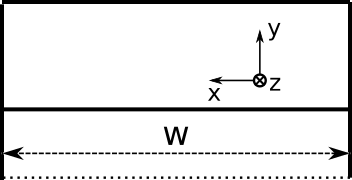
\includegraphics[width=\textwidth]{flat_model.png}
            \caption{Flat transition.}
            \label{fig:flat_transition}
        \end{subfigure}
        \begin{subfigure}[b]{0.24\textwidth}
            \centering
            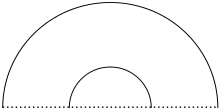
\includegraphics[width=\textwidth]{round_model.png}
            \caption{Round transition.}
            \label{fig:round_transition}
        \end{subfigure}
        \begin{subfigure}[b]{0.5\textwidth}
            \centering
            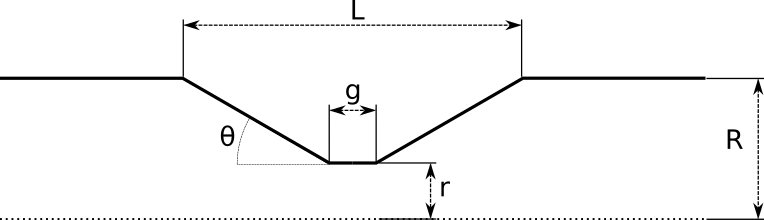
\includegraphics[width=\textwidth]{scheme_collimator.png}
            \caption{Scheme of a tapered transition.}
            \label{fig:collimator_geometry}
        \end{subfigure}
        \caption[Scheme of a tapered transition.]{When $r>R$ the element is called cavity and when $r<R$ it is called collimator. The tapers are the smooth transition regions of the chamber, region where the radius varys. When the transition has no tapers it are called step--in or step--out, depending on the relation between the initial and final radius.}
        \label{fig:collimator_geometry_types}
    \end{figure}
    shows a scheme of such type of geometry, with the important parameters for the impedance calculation. Such geometry can be separated in two independent contributions from the two cross section variations if the gap, $g$, is large, according to~\citeonline{Bane2007}. As discussed by~\citeonline{Heifets1991}, when the beam passes through transitions two forces act on it: one from the change of the energy stored in the synchronous component of the field that travels with the beam, $Z_s$, originated due to the difference in the cross sections, and another one due to the radiation emitted by the image charges on the wall, $Z_r$,
    \begin{subequations}
        \begin{align}
            Z_0^\text{out} &= Z_r + Z_s\\
            Z_0^\text{in}  &= Z_r - Z_s
        \end{align}
    \end{subequations}
    where $Z_0^\text{out}$ is the total impedance of the transition where the beam goes from a smaller chamber to a larger one (step--out), $Z_0^\text{in}$ is the impedance from a larger chamber to a smaller one (step--in) and the equality of the terms $Z_r$ in both cases is a consequence of the beautiful theorem of directional symmetry of the impedance, demonstrated by~\citeonline{Heifets1990}. The term $Z_s$ is constant regardless of the frequency and tapering of the transition, and causes energy gain in the step--in case and energy loss for the step--out. For a transition with round cross--section this contribution to the impedance is given, according to~\citeonline{Palumbo1994}, by
    \begin{align}\label{eq:transition_high_frequency}
        Z_s \approx \frac{Z_0}{2\pi}\ln\fof{\frac{r_1}{r_2}},
    \end{align}
    where $Z_0 = 120\pi$~\si{\ohm} is the impedance of free space and $r_1$ and $r_2$ are the radia of the chamber before and after the transition, respectively. Besides, for the step--in case the total energy loss by the beam must be approximately zero, $Z_0^\text{in}\approx 0$, because the radiation emitted propagates in the opposite direction of the beam. This means that all the energy of the radiation must be taken from the synchronous field, which yelds that in the high frequency limit $Z_r = Z_s$.

    Notice that the average influence of the source term, $Z_s$, on the impedance in one turn around the ring is zero, because of the periodicity of the vacuum chamber. Thus, the term that really matters is the contribution from radiation, which depends on the characteristics of the transition, such as the tapering. Analytic studies of this component were carried out by~\citeonline{Yokoya1990} for a round geometry (Figure~\ref{fig:round_transition}), where the author derived expressions for the low frequency range of smoothly varying tapered transitions. Later \citeonline{Stupakov1996a} corrected the upper frequency limit of the validity of these expressions and extended the lower limit to zero frequency. The result is the following:
    \begin{align}
        \frac{\omega r^2}{cl}\ll1:\quad\quad
        &Z_\parallel = -\frac{i\omega Z_0}{4\pi c}\infint{z}{\fof{r'}^2}, &
        Z_t = -\frac{i Z_0}{2\pi}\infint{z}{\fof{\frac{r'}{r}}^2},
    \end{align}
    where $r=r(z)$ is the radius of the chamber, $r'=r'(z)$ is the derivative of the radius and $l=(L-g)/2$ is the taper length. This impedance is imaginary while the one from the high frequency limit is real. This happens because below the cutoff frequency no radiation can propagate, suggesting that above this threshold a real part of the impedance will arise and approach the high frequency limit, while the imaginary part will tend to zero, after a complex frequency range where the transition between the two limiting behaviors dominates. Another feature of the equation above is that the impedance tends to zero with the taper length. For example, for a linear taper the formulas above simplify to
    \begin{align}
        \frac{\omega r^2}{cl}\ll1:\quad\quad
        &Z_\parallel = -\frac{i\omega Z_0}{4\pi c}\frac{|r_1-r_2|}{t}, &
        Z_t = -\frac{i Z_0}{2\pi}\frac1t|r_1^{-1}-r_2^{-1}|,
    \end{align}
    where $t=\tan^{-1}\theta=l/|r_1-r_2|$ is the transition factor of the taper.

    \citeonline{Stupakov2007a} developed a method to find the low frequency impedance of tapers with general cross sections and derived explicit formulas for a flat taper, consisting on a rectangular geometry with varying vertical gap and constant horizontal apperture, as shown in Figure~\ref{fig:flat_transition}. His results are:
    \begin{subequations}\label{eq:flat_transitions}
        \begin{align}
            \frac{\omega w^2}{2cth}\ll1\,\,\text{and}\,\,h\ll w\ll l:
            \begin{aligned}
                Z_\parallel &= -0.43\frac{i \omega Z_0}{\pi c}\infint{z}{(h')^2}\\[2mm]
                Z_y &= -\frac{i Z_0w}{4}\infint{z}{\frac{(h')^2}{h^3}}\\[2mm]
                Z_x^D&= -Z_x^Q= -\frac{i Z_0}{4\pi}\infint{z}{\fof{\frac{h'}{h}}^2}
            \end{aligned},
        \end{align}
    \end{subequations}
    where $w$ is the chamber half--width and $h(z)$ is the half--gap. It is worth noting that the dipolar horizontal and the quadrupolar impedances are equal to each other and a factor of 2 smaller than the transverse impedance in a conical taper, while the longitudinal impedance is approximately $7/4$ of its counterpart. The most interesting result, however, is the linear dependence of the vertical dipolar impedance with the width of the chamber, which makes this impedance approximately $\pi/2w/\average[\text{harm}]{h}$ larger than the round chamber one. For example, for a linear taper these expressions become
    \begin{align}
        \frac{\omega w^2}{2cth}\ll1\,\,\text{and}\,\,h\ll w\ll l:
        \begin{aligned}
        Z_\parallel &= -0.43\frac{i \omega Z_0}{\pi c}\frac{|h_1-h_2|}{t},\\[2mm]
        Z_y &= -\frac{i Z_0}{2}\frac{w}{t}(h_1^{-1}+h_2^{-1})|h_1^{-1}-h_2^{-1}|,\\[2mm]
        Z_x^D&= -Z_x^Q= -\frac{i Z_0}{4\pi}\frac1t|h_1^{-1}-h_2^{-1}|,
        \end{aligned}
    \end{align}
    where we note that $Z_y^\text{flat}/Z_y^\text{round} = \pi w(h_1^{-1}+h_2^{-1})$.

    \citeonline{Podobedov2007} studied the low frequency limit of confocal\footnote{Confocal ellipses means they have the same \emph{foci}. In the case of the transition cited here, the equation $a^2(z_1)-b^2(z_1)=a^2(z_2)-b^2(z_2)$ is valid for any longitudinal position $z_1$ and $z_2$, where $a$ and $b$ are the larger and smaller axes of the ellipse.} elliptical transitions and found results very similar to the expressions above for the flat geometry, which gives some confidence in trying to extend the qualitative results discussed here for approximated geometries.

    Even though the low--frequency impedance of long and short collimators and cavities are the same, because the equations showed above can be applied to both limits,~\citeonline{Heifets1990} found different limits for the high frequency impedances of a round cavity, depending on the length of their gap. Besides,~\citeonline{Stupakov2007} found equal limit values for the longitudinal impedance, but different for the transverse dipolar impedance in a round collimator. While for the longitudinal limit the value is two times the quantity in equation~\eqref{eq:transition_high_frequency}, for the transverse plane they found
    \begin{align}
        \text{short:}\quad Z_x^D = \frac{Z_0c}{2\pi\omega r^2}\fof{1-\frac{r^4}{R^4}} &&
        \text{long:}\quad Z_x^D = \frac{Z_0c}{\pi\omega R^2}\fof{1-\frac{R^4}{r^4}}
    \end{align}
    where the notation of Figure~\ref{fig:collimator_geometry} was used. Besides, there is a very large frequency gap between the two limiting cases that are of great importance, mainly for storage rings such as Sirius, which have bunche lengths that sample these frequencies. For the round collimator, \citeonline{Stupakov2010} used the parabolic equation to calculate the impedance from a few dozens \si{\giga\hertz} up to a few \si{\tera\hertz}, with excellent agreement with results from numerical solvers. However, so far the impedance for other geometries, or even the detailed behavior of one of the round transitions, can only be accessed with the aid of numerical solvers.

    For example,~\citeonline{Blednykh2006} studied the impedance of the flat collimator--type chamber of a mini--gap undulator and found very intense narrow--band mode just above the cutoff of the pipe, that depended very strongly on the width of the cross--section. For all these reasons the formulas studied here, even though very useful to the study of this type of impedance and qualitative analysis of the relevant parameters for impedance optimization, will not be used quantitatively for any device of the impedance budget.

\subsection{Multi--layer Resistive Wall}

    The standard resistive wall effect has been known for a long time. It was first observed to generate coherent oscillations in electron streams coupled to circuits by \citeonline{Pierce1951} and then used to create a resistive-wall amplifier by \citeonline{Birdsall1953}. This idea was first applied to the study of collective effects in accelerators by \citeonline{Neil1965} and \citeonline{Laslett1965} to explain longitudinal and transverse coherent oscillations of coasting beams and then by \citeonline{Courant1966} to describe instabilities of bunched beams. Since then the theory for calculation of the now called resistive-wall impedance evolved~\cite{Chao1993}, being exactly solved by \citeonline{Bane1991} for a round and infinitely thick and long vacuum chamber, where the author provided analytic formulas for the short-range wake-fields, and for an arbitrary transverse cross section by \citeonline{Yokoya1993}, who based its work on a formalism developed by \citeonline{Gluckstern1993}. In his work, \citeauthor{Yokoya1993} also showed that the spectral dependency of the longitudinal and transverse dipolar and quadrupolar impedances of elliptic chambers with equal smaller axis, but different eccentricities, are identical, in such a way that their wake functions differ from each other only by a constant factor. In the special cases of a round and a flat chamber, which are degenerated cases of an ellipse, with eccentricities equal to $0$ and $1$ respectively, the so called \citeauthor{Yokoya1993} factors are given by
    \begin{align}
        \fof{Z_\parallel}_\text{flat} &=
                        \fof{Z_\parallel}_\text{round}\\
        \fof{Z_x^D}_\text{flat} &= \frac{\pi^2}{24}
                        \fof{Z_x^D}_\text{round}\\
        \fof{Z_y^D}_\text{flat} &= \frac{\pi^2}{12}
                        \fof{Z_x^D}_\text{round}\\
        \fof{Z^Q}_\text{flat} &= \frac{\pi^2}{24}
                        \fof{Z_x^D}_\text{round},
    \end{align}
    where the net horizontal force felt by the witness particle with the same horizontal position as the source particle is zero for the flat chamber. Actually, this is a particular case of the general result that the wake potential of this structure must not depend individually on the horizontal positions of the source and witness particles, but only on their difference
    \begin{align}\nonumber
        W_\text{flat}(x_s,y_s,x_w,y_w,z)=W_\text{flat}(y_s,y_w,x_s-x_w,z),
    \end{align}
    so that the condition of translational symmetry in the horizontal direction is respected.

    It is very recurrent in accelerators to have chambers that are composed of different laminar layers of materials. For example, the chambers of fast time-varying magnets, such as the injection kickers of a storage ring, must be made of a bad conductor, generally a ceramic, to allow the penetration of the fields. To avoid discontinuities in the path of the image current of the beam\footnote{This is equivalent to say: "to decrease the impedance of the beam".}, which could lead to excessive heating and consequent melting or burning of the magnet components and the accumulation of static charges in the ceramic, a thin layer of metal is coated in the inner surface of the chamber. The thickness of the coating must be of a few microns: thin enough not to distort the external field as it penetrates the walls, which has frequencies of the order of hundreds of kilo Hertz, and thick enough to shield most of the frequencies of the beam, which extend to a few dozens of giga Hertz. Especifically for the kicker magnet, outside the ceramic vacuum chamber, there is a layer of ferrite, which is used to guide the external field of the kicker. In the low frequency part of the spectrum, all these different layers of materials are seen by the self--generated fields of the beam and contribute to the impedance.

    Besides, the multi--layer chamber model also applies in the simple case of a standard vacuum chamber of an accelerator, where the finite thickness of wall can be interpreted as a multi--layer chamber composed of metal and air. For low frequencies, the skin depth of the material becomes larger thatn the thicness of the chamber, which decreases the losses by the beam. As a consequence, the real part of the impedance goes to zero and the imaginary part goes to a constant value as the frequency tends to zero. This behavior is correctly predicted by the multi--layer model, while the infinitely thick formula predicts that both impedances diverge to plus and minus infinity, respectively. This low frequency of the resistive wall has a very narrow band nature and influences the long--range wake fields, which are directly related to the coupled bunch resistive--wall instability and the incoherent tunen shifts caused by chambers without circular symmetry, as explained by \citeonline{Chao2002}.

    The multi--layer chambers problem was first tackled by \citeonline{Zotter1969}, who created an algorithm that solved the problem for an arbitrary number of layers of materials with arbitrary electric and magnetic properties, as long as they were linear, homogeneous and isotropic~\cite{Zotter1969,Zotter1969a,Zotter1970}. Even though his method was general enough to be applied to any azimuthal mode $m$ of the source, he only calculated the fields for the azimuthal modes $m=0$ and $m=1$\footnote{It is remarkable that his method goes beyond the rigid beam approximation, considering the source of the wake fields as an infinitely long beam oscilating in the transverse plane to calculate the mode $m=1$.}. This allowed him to derive explicit analytic formulas, under some approximations, for the longitudinal impedance of simplified configurations, such as a single wall with finite thickness, and a metallized ceramic chamber sorrounded by a \gls{pec}. In this latter case, the author concluded that the effectiveness of the coating in the inner wall was much higher than what is intuitively thought by comparing the thickness of the coating with the skin depth of the fields for a given frequency.

    Later \citeonline{Piwinski1977} calculated the impedance generated by a gaussian bunch in a four-layer round chamber composed of metal, ceramic, ferrite and \gls{pec}, in that order, and confirmed what \citeonline{Zotter1970} had previously found: for this type of multi--layer chambers, the fields will not penetrate through the coating if its thickness, $t$, satisfies
    \begin{align}
        t > \frac{\delta^2}{d}, \quad\text{with}\quad
        \delta = \sqrt{\frac{2}{\mu_0\omega\sigma_c}}
    \end{align}
    where $\delta$ is the skin depth, $\sigma_c$ is the conductivity of the coating, $\mu_0$ is the magnetic permeability of vacuum, $\omega$ is the angular frequency of the fields and $d$ is the thickness of the ceramic. This means that, since generally $d\gg t$, the coating is efficient down to frequencies much lower than what is intuitively thought.

    In a more recent work, \citeonline{Zotter2005} rederived his formalism for a point like charge, which was used by \citeonline{Mounet2009} to derive formulas for the electromagnetic fields and impedances of any azimuthal mode $m$, under the assumption of a rigid beam. Later, the same authors also derived expressions for a multi--layer flat chamber with possible different layers in the top and bottom plates~\cite{Mounet2010a} which allowed them to generalize the \citeauthor{Yokoya1993} factors~\cite{Mounet2010}. Then, in his PhD thesis, \citeonline{Mounet2012} developed a general method to perform Fourier integrals, which allowed him to compute the exact short and long--range wake functions using the impedances. All these developments in 2D impedance theory were implemented by \citeauthor{Mounet2011} in a code called ImpedanceWake2D~\cite{Mounet2011} that is available as free software for the accelerator community.
    It is important to mention that other authors also solved the problem of multi--layer impedances using different methods, for example \citeonline{Hahn2008} and \citeonline{Al-Khateeb2005} also derived general methods valid for arbitrary energies and frequencies in round chambers and \citeonline{Burov2002,Burov2002a} also solved the problem under the assumption of long wavelengths, $c/\omega \ll a$, for round and flat geometries.

    In summary, the theory of smooth multi--layer infinitely long round chambers is completely solved. In this work we implemented \citeauthor{Mounet2009} formulas to calculate the impedances for round chambers for the azimuthal modes $m=0$ and $m=1$ in Matlab\textregistered~and Python3 and the wake functions were obtained using the code ImpedanceWake2D. In cases where the eccentricity of the chamber is large, the \citeauthor{Yokoya1993} Factors are applied to the round chamber results.

\subsection{Numeric Methods}\label{ssec:numeric_methods}

    The numerical solvers can be grouped in two categories: 1) the frequency domain codes, that are more indicated for calculation of resonant modes below the cutoff of the chamber, and 2) time domain solvers. While the first class computes the eigen-values and eigen-modes of the structures and the user must identify which ones can be excited by the beam passage, the latter solves \gls{maxeq} computing directly the fields that are generated by the beam. In this type of solvers the beam is modeled by a line density of charge, $\lambda$, that traverses the structure at the speed of light with a constant transverse displacement, $\vect{\rho}'_0$, and then, by discretization of the space-time in grids and approximations of the derivatives by linear operators on the fields in the vertices and faces of each grid, the electromagnetic field can be calculated up to the desired distance behind the source, so the integral defined in equation~\eqref{eq:momentum_gain} can be carried out. Depending on the methods employed in the discretization and the properties of the linear operators in each grid, different convergencies of the solutions related to the finesse of the grids can be achieved. There are several different methods and codes in the literature dedicated to this purpose. For a good review on numeric methods \citeonline{Niedermayer2016} and its references are recommended.

\subsubsection{Finite Line Density Issue}

    This procedure employed to find the impedances has an intrinsic limitation: the line density used as source particle in simulations must allways spread over a few grids, which means a delta-like function can never be used and the wake functions, or wake potential, cannot be obtained. Instead, the effective wake potencial, given by
    \begin{align}
        V(\vect{\rho}'_0, \vect{\rho}, z) = \udefint{z'}{
                \lambda(z') W(\vect{\rho}'_0,\vect{\rho},z-z')},
    \end{align}
    is the result of the simulations. In principle this equation could be inverted with the aid of the convolution theorem~\cite{wiki2017a}, where after the Fourier transform on both sides of the equation one could get
    \begin{align}\label{eq:deconvolution}
        \fourier{W} = \frac{\fourier{V}}{\fourier{\lambda}}.
    \end{align}
    However, this procedure fails to give the values of the impedance at large frequencies due to two effects: the most obvious is the limitations imposed by the Nyquist theorem applied to the grid length of the simulation and the other comes from the fact that the line density Fourier transform has a tail at large frequencies that makes the denominator of equation~\eqref{eq:deconvolution} very small, which, in turn, increases the effect of the noise of the simulations for this frequency range. This limitation on the knowledge of the impedance for high frequencies makes it impossible to obtain the wake function accurately for short distances from the source.

    The line density generally used for such calculations is the gaussian distribution:
    \begin{align}
        \lambda(z) = \frac{1}{\sigma\sqrt{2\pi}}
        \exp\left(-\frac{(z-n\sigma)^2}{2\sigma^2}\right),
    \end{align}
    where $n$ is an integer generally equal to 5 or 6.
    due to its minimal duration-bandwidth product~\cite{Niedermayer2016}. A rule of thumb for these calculations is to consider the impedance only up to frequencies $\omega<=2\sigma/c$ thus avoiding strong influences of the numerical noises as discussed above, which is much more limiting than the Nyquist requirement, given that in simulations the bunch length must be at least five times larger than the grid size.

    The authors \citeonline{Podobedov2013} found a way to overcome this problem, as long as the bunch length used in the simulation is short enough. However, a more practical approach comes from the fact that a real bunch also has a finite length and cannot excite wakes with arbritarely large frequencies, which means if the line density used to obtain the wakes is smaller than the smallest longitudinal structure in the bunch expected to generate any macroscopic significant effect we want to study, then the impedance extracted from that simulation is close enough. Notice this method is intrinsically non-consistent, because we must know \emph{a priori} how the beam will behave to compute the impedance that will drive this behavior. However, the knowlegde gathered by the accelerator physics community in the last fifty years, through several experiments and confrontation of these results with simulated and analytic calculated beam dynamics, led to some rules of thumb that determines the maximum frequency that can be expected to influence the dynamics of a bunch with a given natural bunch length.

    This approach may be conflicting in some situations when the high frequency content of the wake is desired but the structure being analysed has strong resonant modes that take hundreds of meters behind the source to damp. Running a simulation with a short line density will drastically increase the complexity of the simulation because of the smaller mesh size. The solution for these cases is running two simulations, one with a short bunch and small wake length and other with a longer bunch and long wake length, to characterize the resonant mode. Another approach is to simulate the resonant modes with a frequency domain code.

\subsubsection{ECHO Code}

    There are some solvers in the literature that were developed specifically for rotationally symmetric geometries, such as ABCI~\cite{Chin1994a}, since this type of structure is rather common in accelerators. In this type of systems the wake potential in the ultra-relativistic approximation can be partially solved without the need of specifying the boundary conditions, only by the application of the Panofsky-Wenzel theorem and equation~\eqref{eq:potential_harmonic}. It can be shown~\cite{Stupakov2000a} that the most general form for the wake potential in such conditions is:
    \begin{align}
	       W(\rho_s, \rho_w, \theta, z) = \sum_{m=0}^\infty W_m(z) \rho_w^m\rho_s^m\cos(m\theta)
    \end{align}
    where $\rho = |\vect{\rho}|$ is the distance of the particles to the center of the chamber, $\theta$ is the angle between the the source and the witness particles and the source particle is assumed to lie in the $\versor{x}$ direction. The wake functions can be obtained from the gradient of the wake potential. Expanding the wake functions in the leading order we have
    \begin{align}
	    w_s(z) &\approx W'_0(z)\\
	    \vect{w}_t(x_s, z) &\approx W_1\rho_s(\versor{r}\cos(\theta)-\versor{\theta}\sin(\theta)) =
						W_1x\versor{x}
    \end{align}
    where the force is in the same direction that of the displacement of the source particle.

    This partial solution of the wake potential allows us to solve each azimuthal component of the wake potential separatelly, which implies the numerical solution can be found for a single plane of the structure, for example, the plane $x-s$, or $y=0$. This bidimensional mesh drastically reduces the simulation time for such components and this class of codes are called 2D solvers. Among such codes we highlight ECHOz1 and ECHOz2~\cite{Zagorodnov2003, Zagorodnov2005, Zagorodnov2006a}, which are distributed as free software by the author. While ECHOz1 calculates only the azimuthal mode $m=0$, ECHOz2 provides the longitudinal and transverse wake functions for an arbitrary mode $m$.  This code employes several solutions to common problems of numeric simulations that makes it the state of the art for impedance calculation. Among the advantages of this code we highlight:
    \begin{itemize}
	    \item zero dispersion in the longitudinal plane. Longitudinal dispersion is a typical numeric artifact that introduces a non-physical dependency of the phase velocity of the electromagnetic waves with their frequency, which deteriorates the precision of the wakes;
	    \item fast convergence of the ratio between bunch size and grid length, $\sigma/h$: in other codes this ratio must be one order of magnitude larger than ECHO's value for the results to have the same precision. In ECHO a ratio of \SI{5}{} already gives convergent results, which greatly reduces the simulation time for a given frequency requirement on the knowlegde of the impedance;
	    \item moving mesh: instead of discretize the whole structure, the grids move with the source and this region extends behind it only down to the desired length of the wake. This approach helps reducing the simulation time in cases where the structure is larger than the wake length and is applied in other codes too, such as GdfidL;
	    \item indirect integration: for the wake calculation, the infinite integral in the longitudinal direction can be substituted by finite integrals in closed contours that span the structure longitudinally. The first method proposed by~\citeonline{Weiland1983} was valid only for cavity-like structures, but then it was generalized for any rotationally symmetric structure by~\citeonline{Napoly1993}, and finally generalized for any 3D structure by~\citeonline{Zagorodnov2006a}. This procedure greatly reduces the computational time because otherwise it would be necessary to propagate the beam for a very long distance only for the integral to converge. Besides, it improves the precision of the results, because the long integral in the direct method suffers from accumulation of numerical errors.
    \end{itemize}

    There is another code provided by the same author, ECHOzR, that calculates the wakes for structures with rectangular cross sections~\cite{Zagorodnov2015}. The conditions imposed on the geometry are that the lateral walls are composed of infinite vertical and perfectly conducting parallel plates separated by a distance $w$ and that the horizontal walls that define the vertical gap has an arbitrary longitudinal profile and electrical conductivity. Employing the harmonic properties of the wake potential (equations~\eqref{eq:potential_harmonic} and~\eqref{eq:potential_harmonic_source}) on the transverse coordinates of the source and witness particles, the author solves partially the wake potential by expanding it in trigonometric functions that automatically satisfy the boundary conditions in the vertical plates. This way, similarly to the rotationally symmetric case, the numerical computation is reduced to a bidimensional problem that is solved independently for each term of the expansion. All the advantages presented for ECHOz2 regarding the precision of the results and simulation time also applies for ECHOzR. The main difference between the two codes is that for the rectangular code significant post-processing of the results is needed, because the lowest order longitudinal and transverse wake functions are an infinite sum of the modes of the expansion. However, close to center of the chamber, convergence can be achieved by summation of approximately the first ten modes. In Appendix~\ref{app:wake_from_echozr} we discuss on the post processing necessary to retrieve the wakes from the simulation data.

    There is also a generic version of the ECHO code, called ECHO3D, that can be used to compute the wakes for an arbitrary geometry. This code has all the advantages of the bidimensional codes, but lacks a key feature: it is not parallelized. For 3D structures this limitation imposes great restrictions on the type of simulation that can be performed, due to the extremelly large required computational time.

\subsubsection{GdfidL Code}

    When the components of the vacuum chamber do not respect the symmetries required by the 2D solvers or cannot be approximated by one that does, 3D codes must be used. They are also used when a detailed simulation is needed to compute not only the wake potential but also the distribution of the electromagnetic field density in the structures, to calculate heating effects and also the transmission of the fields through ports. The most well-known applications for this type of simulations are GdfidL~\cite{Bruns1997, Bruns2017} and CST Particle Studio~\cite{CST2017}, being the first code the adopted choice for Sirius components design and simulation. In Appendix~\ref{app:wake_from_gdfidl} we discuss on the post-processing of GdfidL computation data.


%%%%%%%%%%%%%%%%%%%%%%%%%%%%%%%%%%%%%%%%%%%%%%%%%%%%%%%%%%%%%%%%%%%%%
%%%%%%%%%%%%%%%%%%%%%%%%%%%%%%%%%%%%%%%%%%%%%%%%%%%%%%%%%%%%%%%%%%%%%
\chapter{Collective Effects}\label{cap:collective_effects}

    In the previous chapter the mechanism of interaction between particles was modeled and formulas for the momentum change of an arbitrary particle due to the action of all the other particles in the beam were derived. In this chapter we will try to include these interactions in the dynamic model of the particles and analyze how the beam will behave as a whole.

\section{Sum of the Wakes}\label{sec:sum_of_wakes}

    With the theory developed so far it is formally possible to calculate the wake potential for all the structures of the ring and include their effects on the beam dynamics assuming the impulse approximation, which considers the variation of the particle momentum must be applied at the position in the ring equivalent to the center of the impedance source. However, a further approximation is usually done for the calculation of the effect of wake-fields in global parameters of the machine, such as tune--shifts, energy loss and even instabilities. This approximation considers all the impedance sources are located at a single point in the ring, in other words, it neglects the phase advances between each wake source. This way the total longitudinal wake of a machine can be given by:
    \begin{align}\label{eq:scaling_longitudinal}
        W'_0(z) = \sum_i \fof{W'_0(z)}_i
    \end{align}
    where $i$ refers to the $i$-th impedance source of the ring.

    For the transverse plane it is important to remember that the transverse amplitude of the displacements of the source and witness particles varies along the ring, which means the transverse components of the wake potential must be scaled according to the local betatron functions at their positions
    \begin{align}\label{eq:scaling_transverse_general}\nonumber
        W_u^D &=\frac{1}{\fof{\beta_u}_T} \sum_i \sqrt{\fof{\beta_u}_i^s\fof{\beta_u}_i^w}\fof{W_u^D(z)}_i \\
        W_u^Q &=\frac{1}{\fof{\beta_u}_T} \sum_i \fof{\beta_u}_i^w\fof{W_u^Q(z)}_i
    \end{align}
    where $u$ represents $x$ or $y$, $\fof{\beta_u}_T$ refers to the value of the betatron function at the position where all the impedances are being lumped, $\fof{\beta_u}_i^w$ is the value of the betatron function at the location where the witness particle feels the kick and $\fof{\beta_u}_i^s$ is the betatron function where the source particle generated the wake.

    This scaling can be easily understood by the analysis of the wake potential terms of the quadrupolar and dipolar wakes. For example, the horizontal dipolar term of the wake potential corresponds to $x_sx_wW_x^D(z)$, which means it depends linearly on the displacement $x_s$ at the point $a$ where it induces the wake fields. If we want to displace the position where this wake was generated from positions $a$ to $b$ and, on average, keep its value unchanged, it is necessary to consider that the amplitude of movement of the source particle were $\sqrt{\beta_x^a/\beta_x^b}$ larger when it excited the fields and we have to multiply our equivalent wake function by this value. In the same way, the witness particle felt the fields generated by the source at a position $c$ downstream from the point where they were generated and, if we want to consider the position of the witness particle in $b$, it is important to multiply the effective wake by $\sqrt{\beta_x^c/\beta_x^b}$, to keep the average strength unchanged.

    All references in literature consider that the position where the wake is generated and the position where the particles feel these wakes are the same, so in this work we will consider it too. Under such condition, the equations~\eqref{eq:scaling_transverse_general} reduce to
    \begin{align}\label{eq:scaling_transverse_general}\nonumber
        W_u^D &=\frac{1}{\fof{\beta_u}_T} \sum_i \fof{\beta_u}_i\fof{W_u^D(z)}_i \\
        W_u^Q &=\frac{1}{\fof{\beta_u}_T} \sum_i \fof{\beta_u}_i\fof{W_u^Q(z)}_i
    \end{align}
    where $\fof{\beta_u}_i$ is the value of the betatron function at the position of the wake source. However, as seen in Appendix~\ref{app:causality}, depending on the transverse sizes of the chamber the fields can only catch up with the witness at distances of the order of centimeters away from the point where the fields were generated. For \gls{4gls}, where the focusing is very strong, such a distance is enough for the betatron function to have changed considerably. The effect of this consideration can be a topic for future studies.

\section{Energy Loss}\label{sec:energy_loss}

    One of the most important effects of wake fields is the energy loss by the beam. It can be computed considering only the leading order term in the momentum change expansion
    \begin{align}
        \Delta E \approx c\Delta p \approx c\fof{\frac{p_s}{p}\Delta p_s + x'\Delta p_x + y'\Delta p_y} \approx c\Delta p_s.
    \end{align}
    This way the energy variation of a given particle due to wake-fields depends on which bunch it is and on its longitudinal deviation from the synchronous particle and is given, in the most general form, by equation~\eqref{eq:general_eff_long_wake} multiplied by the average charge of the bunches and the charge of the particle. If we consider the distributions are stationary and the ring is uniformly filled with charge, then the expression for the wake-potential is reduced to equation~\eqref{eq:impedance_interpretation_long}.

    Under this approximation, the energy variation of a particle after passing through the impedance source would be given by:
    \begin{align}\label{eq:part_energy_loss}
	  	\Delta E\fof{z} = -eI_bT_0V_0(z) = -eI_bT_0\frac{M\omega_0}{2\pi} \sum_{p=-\infty}^\infty \fourier{\lambda}(pM\omega_0)Z_\parallel(pM\omega_0)e^{-ipM\omega_0 z/c}.
    \end{align}
    where $I_b=Q_b/T_0=N_be/T_0$ is the current per bunch, $T_0$ is the revolution time, $N_b$ is the number of particles per bunch and $e$ is the absolute value of the elementary charge of the electron. The average total energy lost by one bunch is given by
    \begin{align}\label{eq:energy_loss_bunch}
        \average[b]{\Delta E} = N_b\infint{z}{\lambda\fof{z}\Delta E\fof{z}} = -\fof{I_bT_0}^2\overbrace{\frac{M\omega_0}{2\pi} \sum_{p=-\infty}^\infty |\fourier{\lambda}(pM\omega_0)|^2\real{Z_\parallel(pM\omega_0)}}^{\kappa_\parallel}
    \end{align}
    where $\kappa_\parallel$ is called the longitudinal loss factor, $|\fourier{\lambda\fof{\omega}}|^2 = \fourier{\lambda}\fof{\omega}\fourier{\lambda}^*\fof{\omega}$ must be an even function of the frequency, given that $\lambda$ is real. Notice that only the real part of the impedance contributes to the energy loss, because the imaginary part is an odd function of the frequency. The average energy loss per particle can be defined as
    \begin{align}
        \average[p]{\Delta E} = \frac{\average[b]{\Delta E}}{N_b} = -eI_bT_0\kappa_\parallel.
    \end{align}
    For impedances that vary smoothly with the frequency compared to the interval $M\omega_0$, the sum in the definition of the loss factor can be replaced by an integral
    \begin{align}
        \kappa_\parallel =
            \frac{1}{2\pi} \infint{\omega}|\fourier{\lambda}(\omega)|^2\real{Z_\parallel(pM\omega_0)} =
            \frac1\pi \defint{\omega}{|\fourier{\lambda}(\omega)|^2\real{Z_\parallel(pM\omega_0)}}{0}{\infty}.
    \end{align}

    The sum of the energy loss in each impedance source of the ring results in an additional energy loss per turn for the particles. This means the new fixed point of the longitudinal one turn map is not given by equation~\eqref{eq:synchronous_phase_condition}, but by
    \begin{align}
        V(z_0) = U_0 + \average[p]{\Delta E}
    \end{align}
    instead, where $z_0$ is the new synchronous position, measured in relation to the zero current one.

    Another important parameter to consider in the design of several components of the vacuum chamber is the power deposited in the wall per unit area by the beam due to wake fields. To calculate such quantity we need the power loss of the whole beam, which is obtained from equation~\eqref{eq:energy_loss_bunch} by multiplying it by the number of bunches and dividing by the revolution time of the ring,
    \begin{align}\label{eq:total_power}
        P_w = \frac{\average[T]{\Delta E}}{T_0} = \frac{M}{T_0}\average[b]{\Delta E} =
        T_0\frac{I_0^2}{M}\kappa_\parallel
    \end{align}
    where $I_0=MI_b$ is the total current stored. Now, to compute the power density one needs to know the distribution of the tangential component of the electric field on the walls of the geometry. For complex geometries simulated in numerical solvers, this is done automatically by the codes, through the computation of the tangential magnetic field and application of the Leontovich boundary conditions~\cite[pp. 280]{Landau1961} to get the tangential electric field. When the calculation is performed analytically, not only the impedance, but also the fields in all regions of space must be known. For the round chamber, the symmetry helps and the power per unit area, $D_s$, is given simply by
    \begin{align}\label{eq:power_density_circle}
        \fof{D_s}_\text{circle} = \frac{P_w}{2\pi b L}
    \end{align}
    where $L$ and $b$ are the length and radius of the chamber. For flat chambers, which can be approximated by two infinitely large parallel plates, this problem was solved by~\citeonline{Piwinski1992}, whose results were used by~\citeonline{Nagaoka2006} to derive a formula that relates the power density of the parallel plates, at a distance $b$ from the particle, with the one from the round chamber,
    \begin{align}\label{eq:power_density_flat}
        D_s(x) = \frac{\pi^2}{4\cosh^2\fof{\frac{\pi x}{2b}}}\fof{D_s}_\text{circle},
    \end{align}
    where $x$ is the transverse position on the plate from the point of minimum distance between the particle and the plate. This function has a maximum value of \SI{2.5}{} at $x=0$ and decays to negligible values above $x\approx4b$.

\section{Current dependent Hamiltonian}

    The usual approach to calculate the effects of the wakes on the beam is by introducing the total wake potential of the machine in the one turn averaged Hamiltonian~\cite{Berg1996,Lindberg2016}. This is justified by the fact that the wake forces are weak and their effects on the beam are very slow, in such a way that the evolution of the beam parameters are counted in a turn by turn basis. In section~\ref{sec:sum_of_wakes} it was defined a method to sum all the wakes of the machine and the average transverse Hamiltonian was defined in section~\ref{sec:chromaticity}, especifically in equation~\eqref{eq:average_transverse_hamiltonian}, and the average longitudinal Hamiltonian was defined in subsection~\ref{ssec:potential_well}, by equation~\eqref{eq:longitudinal_hamiltonian}.

    The wakes strongly couple the evolution of the transverse dynamics with the longitudinal plane and for this reason, the transverse analysis of collective effects usually deal with the longitudinal Hamiltonian too. On the other hand, the coupling between both transverse planes is very small in normal conditions of machine operation and the wakes do not change this scenario, because of the generally weak coupling contributions from the impedance budget, due to the symmetries of the vacuum chambers. This property allows the simplification of the problem by neglecting the degrees of freedom of one transverse plane when the analysis of the other is being carried out. The analysis of the longitudinal motion is again simplified, without the need of considering both transverse degrees of freedom of the particles. With these considerations, the one turn Hamiltonian of the particles that is generally considered for collective effects studies is
    \begin{align}\label{eq:current_depend_hamiltonian}
        H_n = J_u\fof{\nu_u + \xi_u\delta + J_u\frac{A_{xx}}{2}} +
                H_{\parallel} - \frac{\average{I}T_0V_n\fof{u, z, s}}{(E_0/e)L_0}
    \end{align}
    where $\average{I}T_0$ is the average charge per bunch, the subscript $n$ indicates the $n$--th bunch and the effective wake potential is given according to the ideas developed in section~\ref{sec:potential_of_bunch}, specifically by equations~\eqref{eq:general_eff_wakes},
    \begin{align}\label{eq:generalwake}
        V_n\fof{u, z, s} =\nonumber \sum_{l\in\mathscr{B}}\frac{I_l}{\average{I}}\sum_{k=-\infty}^\infty\udefint{z'}{
        &\left(\lambda_l(z'; s - s_r) W_0(z-z' + s_r) + \vphantom{\frac{u^2}{2}}\right.\\\nonumber
        &\hphantom{u}ud_l(z'; s -s_r) W^D_u(z-z' + s_r) +\\
        &\left. \frac{u^2}{2}\lambda_l(z'; s - s_r) W^Q(z-z' + s_r)\right)},
    \end{align}
    where $s_r$ is the retarded position defined in equation~\eqref{eq:retarded_time_definition}, $\lambda_l$ and $d_l$ are the longitudinal distribution and dipole moment of the beam, defined in equations~\eqref{eq:definition_long_distributions}, and $W_0$ is the primitive function of the longitudinal wake, $W'_0$.

\section{Potential-Well Distortion}

    All the effects of the wakes on the beam can be calculated from the Hamiltonian defined in equation~\eqref{eq:current_depend_hamiltonian}. One particular effect is the distortion of the potential well created by the RF cavities, which changes the equilibrium distribution of the particles and the intrabunch dynamic properties such as the synchrotron tune.

    To calculate such effect, we consider a static distribution for the beam and neglect the effects of $W^D_u$ and $W^Q$, because they are small for a well centered beam in the vacuum chamber. Besides, apart from the effect of cavities, which will be discussed in Appendix~\ref{app:passive_landau_cavity}, the distortions are dominated by short--range wakes, in such a way that we can neglect the multi--bunch and multi--turn contributions. Under such considerations, the Hamiltonian of the particle becomes
    \begin{align}
        H = \frac\alpha2\delta^2 + U(z) -
            \frac{I_bT_0}{(E_0/e)L_0}\udefint{z'}{\lambda(z') W_0(z-z')},
    \end{align}
    which is time--independent. Following the same reasonings performed in section~\ref{ssec:fokker_planck_equation} we notice that equation~\eqref{eq:equilibrium_distribution} is still valid if we substitute the expression for the longitudinal distribution by
    \begin{gather}\label{eq:haissinski_equation}
        \lambda(z) = \mathcal{H}(\lambda,z) \coloneqq A\exp\fof{\frac{1}{\alpha\sigma_\delta^2}\fof{
            -U(z) + \frac{I_bT_0}{(E_0/e)L_0}\udefint{z'}{\lambda(z') W_0(z-z')}}},\\\nonumber
            \text{with}\,\,A \in \mathbb{R} \left| \infint{z}{\mathcal{H}(\lambda,z)}=1\right.,
    \end{gather}
    which is a transcendental integral equation for the longitudinal distribution. This equation was first proposed and solved by \citeonline{Haissinski1973} and for this reason carries his name. Even though analytic solutions exist for some special impedances, such as the one presented by~\citeonline{Shobuda1999}, in general it must be solved numerically.

    The method we adopted to solve this equation was based on an iterative approach. Starting from a very low $I_b$ and an initial guess
    \begin{align}
        \lambda_0^{I_b}(z) = A\exp\fof{-\frac{U(z)}{\alpha\sigma_\delta^2}},
    \end{align}
    we iterate
    \begin{align}
        \lambda_n^{I_b}(z) = \left\{
        \begin{matrix}
            \mathcal{H}(\lambda_0^{I_b},z)       & \quad \text{if } n = 1\\[2mm]
            \mathcal{H}\fof{\frac{\lambda_{n-1}^{I_b} + \beta\lambda_{n-2}^{I_b}}{1+\beta},z} & \quad \text{if } n > 1
        \end{matrix}\right.,
    \end{align}
    where $\beta$ is a positive convergence control variable. For each iteration the difference
    \begin{align}
        d_n^{I_b} = \infint{z}{\fof{\lambda_n^{I_b}-\lambda_{n-1}^{I_b}}^2}
    \end{align}
    is calculated and compared to a threshold, $\epsilon$. When $d_{n_c}^{I_b}<\epsilon$, convergence is assumed and we set $\rho^{I_b} = \rho_{n_c}^{I_b}$. Then, the current is incremented by a small value $I_b + \Delta I$, with $\Delta I \ll I_b$, and the process is repeated with the initial guess $\rho_0^{I_b+\Delta I} = \rho^{I_b}$. This method does not require the wakes to respect causality and can also be applied to generic RF cavity potentials. The current version of the code implemented cannot handle wake functions that are given by distributions, such as the Dirac's delta function, $\delta(z)$, and its derivative, $\delta'(z)$, which corresponds to the resistive and the inductive wakes, respectively, but it could easily be extendend to manipulate such operators. Currently, when we want to simulate these wakes, the effective wake given by the convolution of these distributions with a small gaussian beam is used.
    For example, in the Sirius simulations, where the bunch length is of the order on a few millimeters, a gaussian bunch of approximately $\sigma_z=20$~\si{\micro\meter} is more than enough to reproduce the results of the $\delta(z)$ and the $\delta'(z)$ wakes.

    This implementation was benchmarked with the results presented by~\citenum{Bane1989} for the inductive and resistive impedances. For the capacitive (positive inductance) the code fails to converge when the strength of the perturbation gets close to the well known singularity point of such impedance, as explained by~\citeonline{Shobuda1999}. However this was not a problem for all the practical cases studied in this work.

\section{Incoherent Tune--shifts}\label{sec:incoherent_tune_shift}

    Another effect derived from of the Hamiltonian of equation~\eqref{eq:current_depend_hamiltonian} is the variation of the transverse oscillation frequency of the bunch as a function of the current,
    \begin{align}
        \Delta\nu_u^n = \frac{(\Delta\mu'_u)^n}{\omega_0/c} = \frac{1}{\omega_0/c}\left(\left.\derpar{H_n}{J_u}\right|_{\average{I}} - \left.\derpar{H_n}{J_u}\right|_{\average{I}=0}\right)
    \end{align}
    where the superscript $n$ was used because the tune--shift is different for different bunches if the filling pattern is not uniform and the wakes that generates it are multi--turn effects. Considering the distributions are in equilibrium, we can show that
    \begin{align}
        \Delta\nu_u^n = \frac{\average{I}T_0}{2\pi(E_0/e)}
        \sum_{l\in\mathscr{B}}\frac{I_l}{\average{I}}\sum_{k=-\infty}^\infty\udefint{z'}{
        &\left(\sqrt{\frac{\beta_u}{2J_u}}\cos(\mu_u)d_l(z') W^D_u(z-z' + s_r) +\right.\\
        &\left.\phantom{\sqrt{\frac{1_1}{1_1}}}\beta_u\cos^2(\mu_u)\lambda_l(z') W^Q_u(z-z' + s_r)\right)},
    \end{align}
    where $u = \sqrt{2J_u\beta_u}\cos(\mu_u)$. Notice that for a well centered beam $d_l=0$ and the dipolar wake does not influence the tune, and even in the case when the beam is off centered its average effect is zero, because of the term $\cos(\mu_u)$ that averages to zero for each particle in the beam. The quadrupolar wake, on the other hand, creates a $z$ dependent tune--shift in the beam
    \begin{align}
        \Delta\nu_u^n = \beta_u(1+\cos(2\mu_u))\frac{\average{I}T_0}{4\pi(E_0/e)}
        \sum_{l\in\mathscr{B}}\frac{I_l}{\average{I}}\sum_{k=-\infty}^\infty\udefint{z'}{
        \lambda_l(z') W^Q_u(z-z' + s_r)}
    \end{align}
    Considering an uniform filling patern, with $M$ equal bunches equally spaced, we can follow the reasonings presented in subsection~\ref{ssec:relation_with_impedance} and use equation~\eqref{eq:impedance_interpretation_quad} to show that
    \begin{align}
        \Delta\nu_u = -\beta_u(1+\cos(2\mu_u))\frac{I_bT_0}{4\pi(E_0/e)}
        \frac{iM\omega_0}{2\pi} \sum_{p=-\infty}^\infty \fourier{\lambda}(pM\omega_0)Z^Q_u(pM\omega_0)e^{-ipM\omega_0 z/c},
    \end{align}
    where $I_b$ is the current per bunch. Averaging this result with the bunch distribution and using the impedance property described in equation~\eqref{eq:impedance_even_odd_trans}, we get
    \begin{align}\label{eq:incoherent_tune_shift}
        \average{\Delta\nu_u} = \beta_u\frac{I_bT_0}{4\pi(E_0/e)}
        \overbrace{
        \frac{M\omega_0}{2\pi} \sum_{p=-\infty}^\infty |\fourier{\lambda}(pM\omega_0)|^2\imag{Z^Q_u(pM\omega_0)}}^{\kappa^Q_u},
    \end{align}
    where $\kappa^Q_u$ is the quadrupolar kick factor. Notice that

\section{Instabilities}
\subsection{Multi-Turn Instabilities}
\subsection{Single-Turn Instabilities}
\section{Analytic Treatment}
\subsection{The Linearized Fokker-Planck Equation}
\subsubsection{Modal expantion}
\paragraph{Head-tail modes}
\subsubsection{Solution for Gaussian Bunches}
\subsubsection{Low Current Limit: Multi-Turn Instabilities}
\subsubsection{High Current Limit: Mode Coupling Instabilities}
\subsection{The Microwave Instability}
\subsection{Strong Head-tail instability}

\section{Tracking Code}\label{sec:tracking_code}

    The structure of the tracking code used is very similar to the one described in Ref.~\citenum{Sa2015}, with the additional feature of including damping and quantum excitation terms for the single particle dynamics. Wake field kicks can be included in two different ways:
    \begin{description}
        \item[General Wakes:] In this case the wakes do not need to respect the causality condition and are passed to the code as interpolation tables. The code uses the \gls{pic} approach, where the total simulation length for the longitudinal direction, $L_c$, is segmented into $N_c$ intervals and the approximate beam distribution is calculated from the number of macroparticles in each cell. Then, the convolution theorem is used to calculate the kick curve\cite{Bassi2016}, which is interpolated according to each particle's position;
        \item[Resonators:] The parameters of the resonators, $(R_s, \omega_r, Q)$, are used as input. The code does not use the PIC approach, each of the $N_p$ macroparticles being simulated interact with each other and the wake is calculated through the sum of the potentials left by each particle in each resonator.
    \end{description}

    In the second method $N_p$ is the only variable to be tested for the result convergence analysis, while for the first method the additional variable $N_c$ is also important. This inconvenience can be avoided if the number of slices is set in such a way that the grid length satifies the Nyquist theorem for the highest relevant frequency of the impedance used in tracking,
    \begin{align} \label{eq:nyquist_theorem}
        \Delta z_c = L_c/N_c > \frac{2}{f_\text{max}}.
    \end{align}

    This code was benchmarked with SPACE\cite{Bassi2016} and Elegant\cite{Borland2000}.


\chapter{Impedance Modeling}\label{cap:impedance_modeling}

    In this chapter the impedance modeling of some storage ring components will be described. The components described below are the ones for which the modeling is not trivial and required detailed analysis of some key aspects. The gathering of all the components and analysis of the whole impedance budget will be performed in the next chapter.

\section{Standard Chamber}\label{sec:standard_chamber}

    Sirius standard vacuum chamber will be made of copper with a round cross-section with \SI{12}{\milli\meter} internal radius, $b$, which is considerably smaller than the chambers of the \gls{3gls}, as shown by~\citeonline{Nagaoka2014}.
    This small chamber does not only affect the resistive wall impedance, which scales with $1/b^3$ for the transverse planes, but also all the other components impedance, because of the proximity of the walls with the beam~\cite{Nagaoka2014}. Besides, the solution adopted for the vacuum in Sirius employs the mixed and concomintant use of localized and distributed pumping, where the last is achieved through coating the vacuum vessel with \gls{neg}~\cite{Benvenuti1998,Prodromides2002}. In 2012 the \gls{lnls} signed a license agreement with \gls{cern} to develop \gls{neg} coating in-house and since then the Vacuum Group has been working on the development of the infrastructure and improvement of techniques for production, deposition and in--situ activation of \gls{neg}, to produce coatings with low surface roughness and good thickness uniformity in all vacuum chambers of the ring, as explained by~\citeonline{Seraphim2015} and~\citeonline{Rocha2017}.

    The presence of \gls{neg} changes the electromagnetic properties of the inner surface of the chamber and contributes to the impedance increase. This effect was first noticed in an impedance measurement made in ELETTRA by \citeonline{Karantzoulis2003}, where the authors described an anomalous increase of the tune--shift with current after the installation of \gls{neg} coated Aluminum chambers for \glspl{id}.~\citeonline{Nagaoka2004} tried to explain the measured results using the multi--layer formulas for the transverse impedance, but quantitative agreement was only obtained using excessively large resistivities for \gls{neg}. Such experimental results created some concern in the community and the effect of the roughness of the inner surface of the chamber was hipotesized as a possible explanation. \citeonline{Nagaoka2007a} studied such an effect when analyzing Soleil storage ring measurements, where the impedance budget of the machine was not enough to account for the bunch lengthening observed, and concluded that the impedance of the measured roughness could not explain the additional impedance necessary to fit the experimental results.

    There are expressions in the literature to estimate the impedance of a rough surface, such as ones of \citeonline{Bane1997}, based on numeric calculations, and of \citeonline{Stupakov1999a}, calculated analytically. Their prediction accounts for an inductive impedance in low frequency, where the characteristic length of the surface protrusions is much smaller than the bunch length, and real impedance for very large frequencies. However, one of the considerations for the derivation of such formulas is that the surface is perfectly conducting, which means all the image charges will flow by the rough surface. It seems reasonable that for finite conductivity chambers, the wall currents will penetrate the material and the effect of the roughness should be even smaller.

    Given all the considerations presented above, the initial model adopted for the standard Sirius vacuum chamber is a round smooth multi--layer and infinite pipe, where three layers are considered: \SI{1}{\micro\meter} of \gls{neg} coating, \SI{1}{\milli\meter} of copper and air to infinity. Table~\ref{tab:wall_impedance_parameters}
    \begin{table}
        \centering
        \caption{Wall Impedance parameters.}
        \label{tab:wall_impedance_parameters}
        \begin{tabular}{lcc}
            \toprule
            Parameter              &   Value    & Unit \\
            \midrule
            Copper conductivity    &   59.0     & \si{\mega\siemens\per\meter}\\
            Copper relaxation time &   27       & \si{\femto\second}\\
            NEG conductivity       &   1.0      & \si{\mega\siemens\per\meter}\\
            NEG thickness          &   1.0      & \si{\micro\meter}\\
            Chamber radius         &  12.0      & \si{\milli\meter}\\
            Chamber thickness      &   1.0      & \si{\milli\meter}\\
            Total Length           &  500       & \si{\meter}\\
            Dipole Length          &  100       & \si{\meter}\\
            Chamber shape          & round      & \\
            \bottomrule
        \end{tabular}
    \end{table}
    shows the values of the main parameters of this model, where one can notice that the value used for \gls{neg} conductivity was \SI{1}{\mega\siemens\per\meter}. This value is the average result of a measurement of the \gls{neg} resistivity as function of the frequency made by ~\citeonline{Koukovini-Platia2014}. Since this measurement was performed for a very short frequency range, only from \SI{10}{} to \SI{11}{\giga\hertz}, and considering that other factors may influence the \gls{neg} conductivity, such as the activation process and aging effects, we calculated the impedance for several values of conductivity, as shown in Figure~\ref{fig:wall_impedance_neg_res}.
    \begin{figure}
        \def \mysize {\textwidth}
        \centering
        \begin{subfigure}[c]{\textwidth}
            \centering
            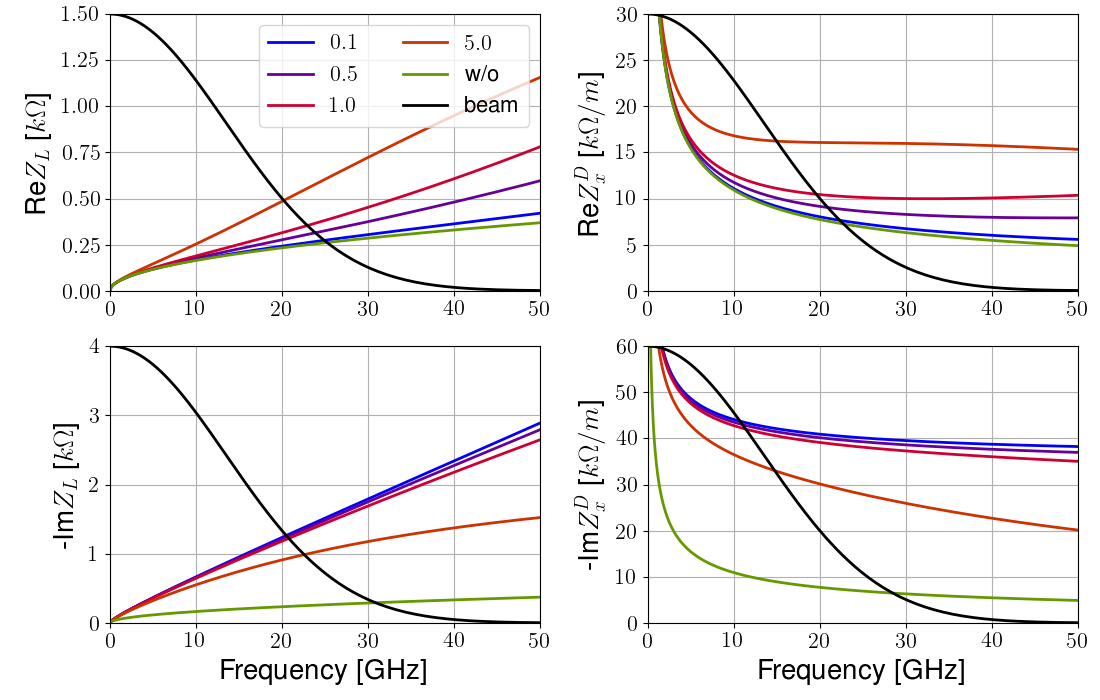
\includegraphics[width=\mysize]{wall_imp_neg_res.png}
            \caption{Wall Impedance as function of \gls{neg} conductivity (in \si{\mega\siemens\per\meter}).}
            \label{fig:wall_impedance_neg_res}
        \end{subfigure}
        \begin{subfigure}[c]{\textwidth}
            \centering
            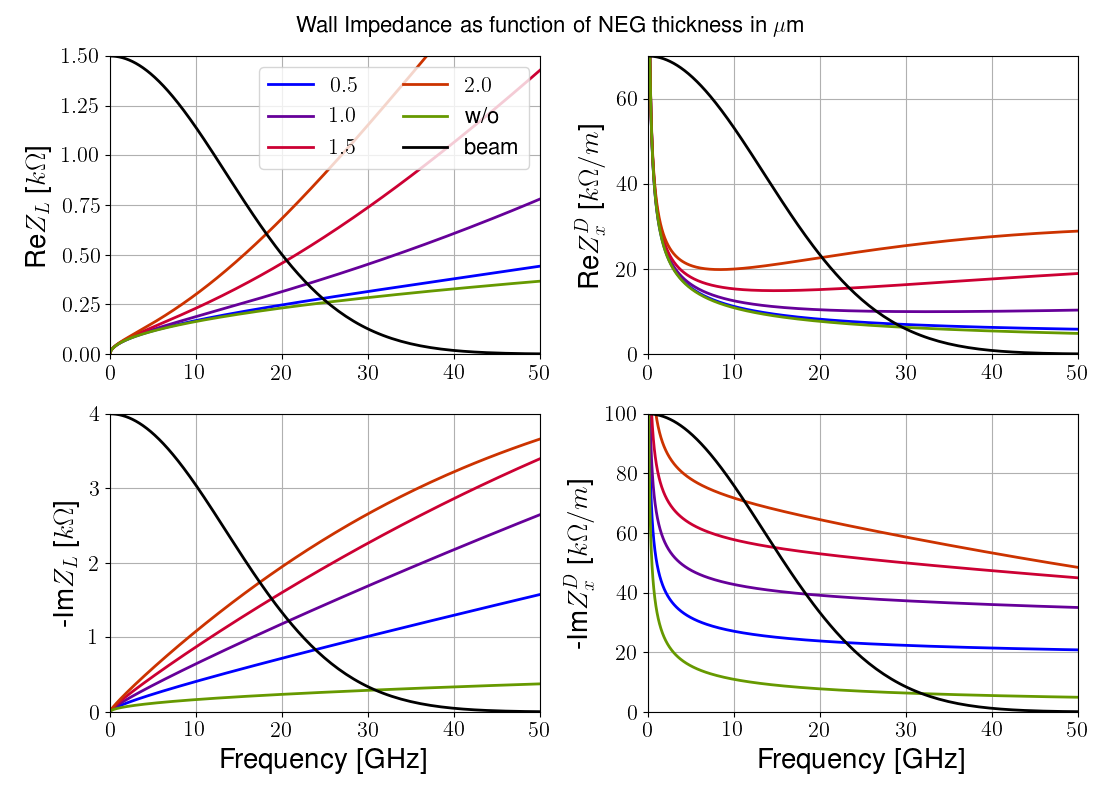
\includegraphics[width=\mysize]{wall_imp_neg_thick.png}
            \caption{Wall Impedance as function of \gls{neg} thickness (in \si{\micro\meter}).}
            \label{fig:wall_impedance_neg_thick}
        \end{subfigure}
        \caption[Neg effect on impedance.]{Wall impedances as function of the frequency for several values of \gls{neg} conductivity (a) and coating thickness (b). The nominal values for both are presented in Table~\ref{tab:wall_impedance_parameters}. Also shown in black is the spectrum of a \SI{2.5}{\milli\meter} gaussian bunch.}
        \label{fig:wall_impedance_neg}
    \end{figure}
    Also shown in the figure is the spectrum, in arbitrary units, of a gaussian bunch with $\sigma=2.5$\si{\milli\meter}, which is the natural bunch length of the Sirius storage ring. Notice that the dependency of the impedance for the frequency range of interest is very non-linear, being almost saturated for lower conductivities, which means that variations on the conductivity does not have a strong impact on the beam behavior. We can also infer from the figure that the effect of \gls{neg} on the impedance is mostly inductive in both planes, where an increase of a factor of \SI{3}{} in the imaginary impedance is noted.

    The increase of the imaginary impedance is clearly evidenciated by Figure~\ref{fig:wall_tmci_neg_res},
    \begin{figure}
        \centering
        \begin{subfigure}[c]{0.49\textwidth}
            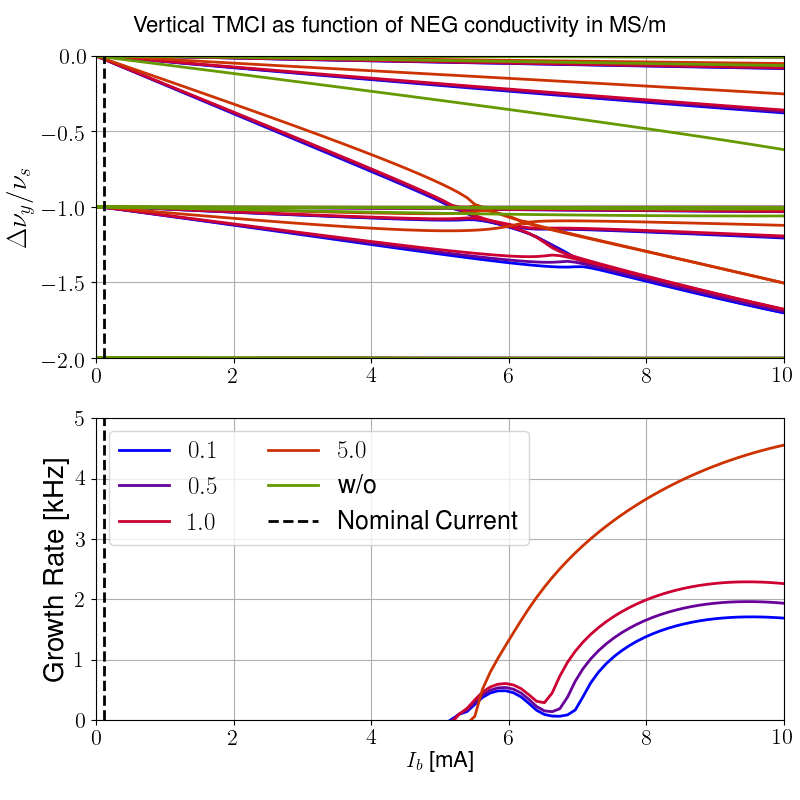
\includegraphics[width=\textwidth]{wall_tmci_neg_res.png}
            \caption{\gls{neg} conductivity in \si{\mega\siemens\per\meter}}
            \label{fig:wall_tmci_neg_res}
            \end{subfigure}\hfill
            \begin{subfigure}[c]{0.49\textwidth}
                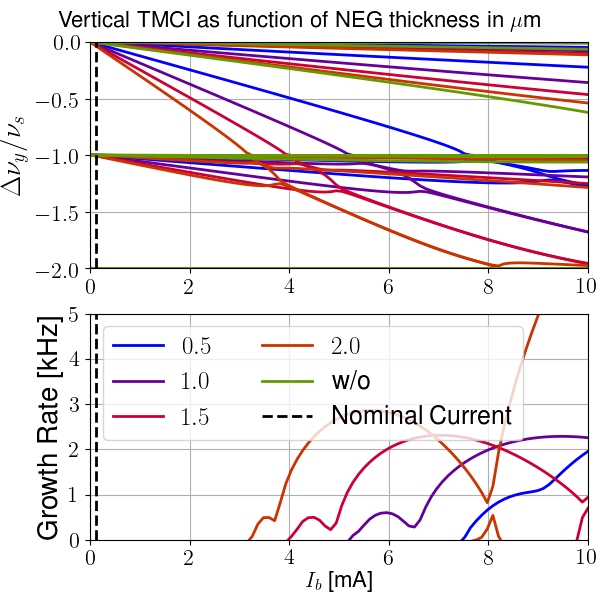
\includegraphics[width=\textwidth]{wall_tmci_neg_thick.png}
                \caption{Coating thickness in \si{\micro\meter}.}
                \label{fig:wall_tmci_neg_thick}
            \end{subfigure}
            \caption[Effect of NEG on TMCI]{Simulations of \gls{tmci} instability for one single bunch in the machine using the parameters of the first phase of operation of the storage ring, as shown in Table~\ref{tab:sirius_main_parameters}, and for several different values of \gls{neg} conductivity (a) and coating thickness (b).}
            \label{fig:wall_tmci_neg}
        \end{figure}
    which shows simulations of transverse single bunch tune-shift and the \gls{tmci} instability, and Figure~\ref{fig:wall_loss_facttor_eff_imp_cond_thick},
    \begin{figure}
        \centering
        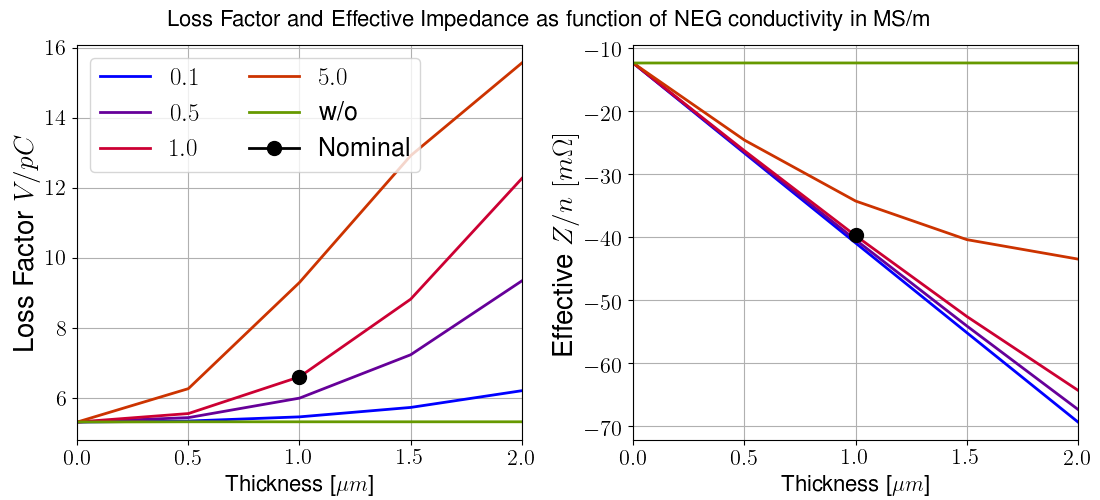
\includegraphics[width=\textwidth]{loss_factor_eff_imp_neg_cond_and_thick.png}
        \caption[Effect of NEG on loss factor and effective longitudinal impedance]{Loss factor (left) and effective longitudinal impedance (right) for a \SI{2.5}{\milli\meter} bunch as function of the coating thickness for several different values of \gls{neg} conductivity, in \si{\mega\siemens\per\meter}.}
        \label{fig:wall_loss_facttor_eff_imp_cond_thick}
    \end{figure}
    which shows the loss factors and the effective longitudinal impedance.

    A study of the impedance dependence on the thickness of the \gls{neg} coating was also carried out, as shown in Figure~\ref{fig:wall_impedance_neg_thick}, Figure~\ref{fig:wall_tmci_neg_thick} and Figure~\ref{fig:wall_loss_facttor_eff_imp_cond_thick}. Differently from the conductivity case, this parameter has strong influence on the value of the impedance, affecting almost linearly the imaginary part in both planes and quadractically the loss factor.

    From the analysis of Figure~\ref{fig:wall_tmci_neg} we note that, even though the \gls{neg} coating has a strong influence on the impedance, the \gls{tmci} threshold induced only by its contribution is much above the nominal single bunch current for uniform filling of the machine and do not compromise the operation. Besides, as will be seen with further details in the next sections, the increased longitudinal inductive impedance will contribute to the bunch lengthening, which helps decreasing \gls{ibs} effects and improve Touscheck lifetime.

    A complete analysis of the impedance of a \gls{neg} coated chamber is provided by \citeonline{Shobuda2017}, who explains the existence of several regimes along the spectrum where different mechanisms majorly defines the impedance behavior. For example, the skin depth of \gls{neg} at \SI{30}{\giga\hertz} is approximately \SI{3}{\micro\meter}, which is three times larger than the thickness of the coating used in Sirius chambers, thus, in the frequency range analysed so far, from \SI{1}{} to \SI{50}{\giga\hertz}, most of the losses happens in the copper chamber and that is why the impedance is mostly inductive. For higher frequencies the \gls{neg} contribution will be resistive, and for lower it will not have any effect on the impedance.

    One particular range of interest for Sirius is the very low frequency part of the impedance, which goes from \SI{0}{\hertz} to a few \si{\mega\hertz}, because in this range two important mechanisms which influence the dynamics of the beam are defined. The first is the traditional resistive--wall instability, defined by the harmonic of the betatron frequency with lowest frequency, being numerically equal to the fractional part of the tune times the revolution frequency. The second is the incoherent tune--shift induced by the quadrupolar impedance, which depends on the zero frequency value of the impedance. This mechanism was introduced in section~\ref{sec:incoherent_tune_shift} and is quantitatively described by equation~\eqref{eq:incoherent_tune_shift}. Considering that the resistive--wall impedance has a very sharp peak at zero frequency, this term has strong influence on the whole sum that defines the tune--shifts, mainly for multi-bunch operations. Actually the infinitely thick wall theory, from \citeonline{Gluckstern1993} and \citeonline{Yokoya1993}, provides divergent results for this tune--shift. \citeonline{Nagaoka2001} solved this problem in explaining measurements at ESRF using a method developed by \citeonline{Heifets1998} and explained in detail by \citeonline{Chao2002}, which employed the concept of the diffusion time of the magnetic field in the chamber to truncate the multi--turn effect of this impedance as a way of considering the finite thickness of the wall. Later, \citeonline{Shobuda2002} showed that such approach is not needed when the impedance already takes into account the finite thickness.

    The impedance at very low frequencies is very difficult to calculate because it depends on what is outside the vacuum chamber, due to the increasingly large skin depth.~\citeonline{Shobuda2002} pointed this possibility out when they tried to explain the tune--shifts observed in KEKB with their finite--thick wall theory. With the multi--layer formulas used in this work it is possible to see the influence of materials outside the chamber on the impedance, as shown Figure~\ref{fig:wall_imp_dipole_distance},
    \begin{figure}
        \centering
        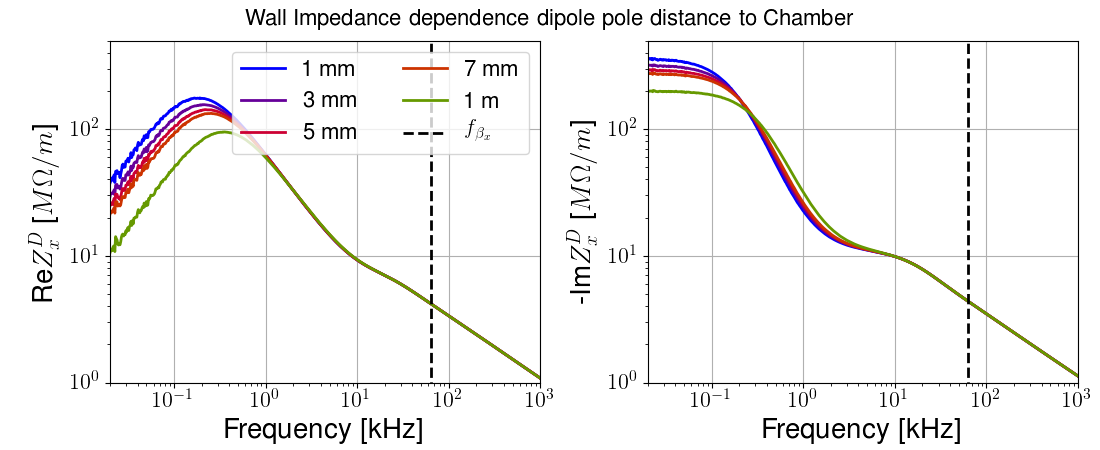
\includegraphics[width=\textwidth]{wall_imp_dipole_distance.png}
        \caption{Low frequency impedance for different values of distance of the magnetic poles of dipoles to the exterior part of the vacuum chamber.}
        \label{fig:wall_imp_dipole_distance}
    \end{figure}
    where the infinitely thick layer of air was substituted by a variable gap of air and a layer of Permendur, used in the magnetic poles of Sirius magnets. Note that the first betatron line, responsible for the coherent tune--shifts and the resistive--wall instability is completely determined by the copper chamber, but the zero frequency impedance depends on the distance of the magnet to the external part of the wall. One can argue that, since Sirius vacuum chamber is round, this dependence is not important because there is no quadrupolar impedance. However, considering that the impedance at these frequencies depend on the materials outside the chamber, it is reasonable to think it will depend on how they are distributed too. Remembering that the storage ring is filled with magnets with cores made out of ferromagnets, and noticing that only dipoles can generate a quadrupolar impedance, because the symmetry of the poles of quadrupoles and sextupoles does not allow such component, we considered this effect on the total budget.

    According to~\citeonline[p. 340]{Zotter1998} the indirect space charge impedance in the ultra-relativistic limit at zero frequency (for penetrating fields) is given by
    \begin{align}\label{eq:space_charge_impedance}
        Z_y = i\frac{Z_0L}{\pi}\fof{(\varepsilon_1-\xi_1)\frac{1}{h_1^2} +
                                         (\varepsilon_2-\xi_2)\frac{1}{h_2^2}}
    \end{align}
    where the indices $h_1$ and $h_2$ refer to the electric and magnetic gaps, respectively, $\varepsilon_i$ and $\xi_i$ are the~\citeonline{Laslett1963} coefficients for incoherent and coherent tune--shifts associated with the electric ($1$) and magnetic ($2$) fields, given by
    \begin{align}\label{eq:laslett_coefficients}
        \begin{aligned}
            &\varepsilon_1 = \varepsilon_2 = 0, & &
            \xi_1 = \xi_2 = \frac12 & &
            \text{for round chambers},\\
            &\varepsilon_1=\frac{\varepsilon_2}{2} = \frac{\pi^2}{48}, & &
            \xi_1 = \xi_2 = \frac{\pi^2}{16} & &
            \text{for flat chambers.}
        \end{aligned}
    \end{align}
    The coherent coefficients, $\xi_i$, are a particular case of the dipolar impedance, while the incoherent coefficients, $\varepsilon_i$, of the quadrupolar impedance. This way, we can intepret the low frequency limit of the impedances show in~Figure~\ref{fig:wall_imp_dipole_distance} as the sum of the electric and magnetic incoherent space--charge impedance. In fact, a direct evaluation of equation~\eqref{eq:space_charge_impedance} for the electric boundary using $h_1$ equals to the internal radius of the vacuum chamber gives an impedance of \SI{208}{\mega\ohm},
    which is very similar to the value of \SI{200}{\mega\ohm} taken from the curve where the magnet is far from the beam. The magnetic part gives a contribution of \SI{117}{\mega\ohm} when we consider the dipole is \SI{16}{\milli\meter} away from the center of the chamber, which corresponds to the curve \SI{3}{\milli\meter} of the graph. This value is also close to the \SI{120}{\mega\ohm}, obtained by the subtraction of the curve \SI{3}{\milli\meter} by the curve \SI{1}{\meter}. With all the considerations above, we defined the quadrupolar impedance for the Sirius vacuum chambers as
    \footnote{As the Sirius dipoles are straight magnets with inclined poles to produce a quadrupole gradient and the chambers, as well as the beam trajectory, are curved along them, the distance of the poles to the chamber is variable. Nevertheless, \SI{3}{\milli\meter} is a good estimate for the average distance and that is why it was used in the definition above.}
    \begin{align}
        Z_y^Q(\omega) = -Z_x^Q(\omega) =
            \fof{\fof{Z_y^D(\omega)}_{\text{round}}^\text{3 mm} -
                    \fof{Z_y^D(\omega)}_{\text{round}}^\text{1 m}}
            \frac{\varepsilon_2^{\text{flat}}}{\xi_2^{\text{round}}} \frac{L_D}{L_T}
    \end{align}
    where $L_T$ is the total length considered for the chamber, $L_D$ is the length covered by dipoles and the fraction involing the \citeauthor{Laslett1963} coefficients is the conversion from the round dipole factor to the flat quadrupole factor. Note that if we had used the \citeauthor{Yokoya1993} factors in the equation above we would get an impedance two times lower. This approach is not correct because this factors were derived under the assumption of infinitely thick chambers, which means they are only valid in the frequency range where the electric and magnetic fields are shielded at the same place, in other words, when they do not penetrate the material.

\section{Kicker Chambers}

    The Sirius storage ring will have two kicker magnets, one standard dipole kicker and one non--linear kicker. While the first will be used for on--axis injection in the commissioning of the light source and as a pinger magnet for machine studies, the second will be used for injection in top-up mode~\cite{Liu2016a}. Even though the topology of both magnets is very different, their vacuum chamber will be identical: a ceramic chamber, coated with \SI{10}{\micro\meter} of Titanium. This means that at high frequencies their impedance will be identical too. Below we describe the considerations on the modeling of the impedance of the dipole kicker magnet and then extrapolate to the case of the non-linear kicker. Table~\ref{tab:kicker_paramters}
    \begin{table}
        \centering
        \caption{Main parameters of the Kicker magnet for impedance modeling}
        \label{tab:kicker_paramters}
        \begin{tabular}{lccc}
            \toprule
            Parameter                     & Symbol    & Value  & Unit \\
            \midrule
            Capacitance                   & $C_{bb}$  &  30.0  & \si{\pico\farad}\\
            Parasitic Resistance          & $R_s$     &  500   & \si{\ohm}\\
            Pulser circuit resistance     & $R_e$     &  50.0  & \si{\ohm}\\
            Ferrite permittivity          &           &   12   & \\
            Ferrite initial permeability  & $\mu_i$   &  1600  & \\
            Ferrite saturation frequency  & $\omega_s$&  20.0  & \si{\mega\radian\per\second}\\
            Ceramic permittivity          &           &  9.3   & \\
            Titanium conductivity         &           &  1.6   & \si{\mega\siemens\per\meter}\\
            FeSi conductivity             &           &  2.0   & \si{\mega\siemens\per\meter}\\
            FeSi permeability             &           & 40     & \\
            \bottomrule
        \end{tabular}
    \end{table}
    shows the main values of the parameters used to model these components.

    Figure~\ref{fig:kicker_magnet}
    \begin{figure}
        \centering
        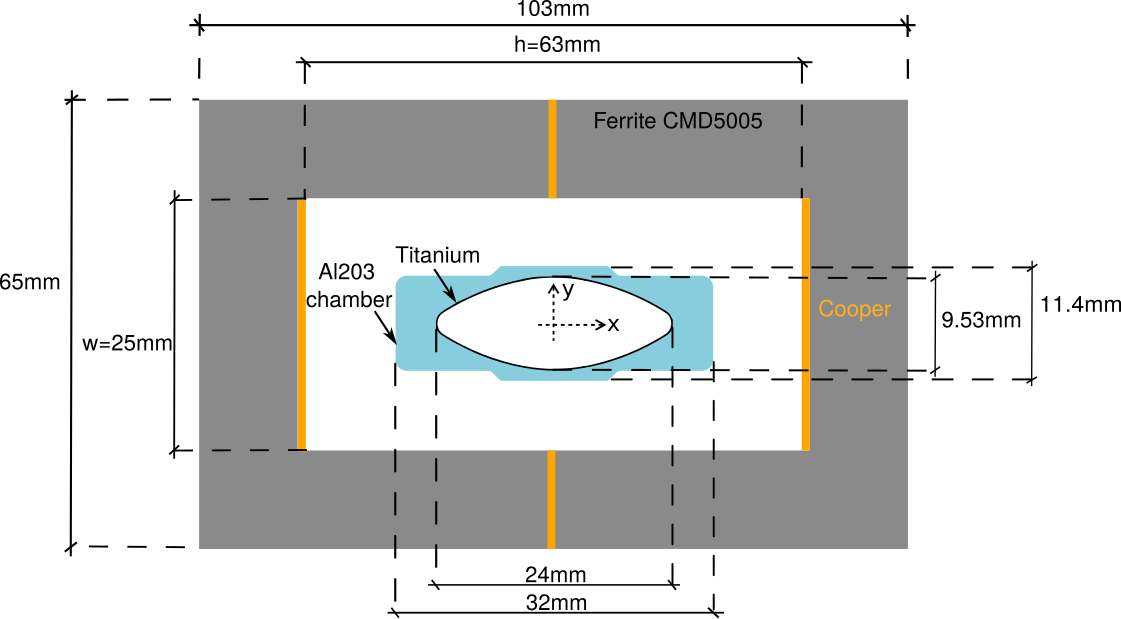
\includegraphics[width=0.8\textwidth]{kicker_magnet.png}
        \caption{Cross section of the kicker window--frame magnet that will be used in Sirius storage ring.}
        \label{fig:kicker_magnet}
    \end{figure}
    shows an schematic drawing of a transverse section of the window-frame dipole kicker magnet that will be used in Sirius storage ring. This type of magnet acts on the beam by the passage of a very strong pulsed current, generated by an external pulser circuit, on the lateral copper plates. This current induces a magnetic field around the plates that is guided by the ferrite to create an almost constant vertical field at the inner gap of the magnet. The copper plates located at the center of the magnet are important to increase the magnetic impedance for the field lines, forcing them to close the loop by the air gap and not around the ferrite blocks.

    There are two main contributions to the impedance of this type of magnet: the losses and resonances defined by the materials of the vacuum chamber and the window-frame itself and the coupled flux of the beam with the external circuit that feeds the magnet. While the first contribution dominates the high frequency part of the spectrum, the second is important at low frequencies.

    The coupled flux, first modeled by~\citeonline{Nassibian1979} and improved by~\citeonline{Davino2003}, treats the window-frame as a transformer that couples the beam with the external circuit impedance, $Z_g(\omega)$, characterized by the impedance termination of the pulser circuit and the residual capacitances and resistances of the device, which can be accessed via twin wire measurements~\cite{Mostacci2016} of the opened and shorted circuits on the endplates, as explained by~\citeonline{Davino2003}. This model predicts impedances for the coupled flux given by
    \begin{align}\label{eq:coupled_flux_impedance}
        Z_\parallel^* = \frac{\Delta^2}{h^2}\frac{i\omega L_2 Z_g}{i\omega L_2 + Z_g},
        & & Z_x^D &= \frac{c}{\omega\Delta^2}Z_\parallel, & & Z^D_y=Z^Q_x = 0
    \end{align}
    where $\Delta$ is a transverse offset of the beam, $L_2 = \mu_0Lh/w$, $L$ is the length of the magnet and $h$ and $w$ are the transverse dimensions defined in Figure~\ref{fig:kicker_magnet}.

    Equation~\eqref{eq:coupled_flux_impedance} predicts zero vertical impedance and, for a well centered beam, $\Delta=0$, the longitudinal impedance is zero too. Considering there is no measurements yet for the circuit impedance, $Z_g(\omega)$, of the kicker magnet, the parametric dependency described by~\citeonline{Davino2003}
    \begin{align}
        Z_g(\omega) = R_e + \frac{1}{\frac{1}{R_s}+i\omega C_{bb}}
    \end{align}
    was used for Sirius, where $C_{bb}$ is the busbar capacitance, equal to \SI{30}{\pico\farad} for their kicker, $R_s$ is a resistance in parallel with the capacitance to account for the ferrite losses, equals to \SI{490}{\ohm} in their case, and $R_e$ is the matching impedance of the external circuit, which we considered equal to \SI{50}{\ohm}. Figure~\ref{fig:coupled_flux_impedance}
    \begin{figure}
        \centering
        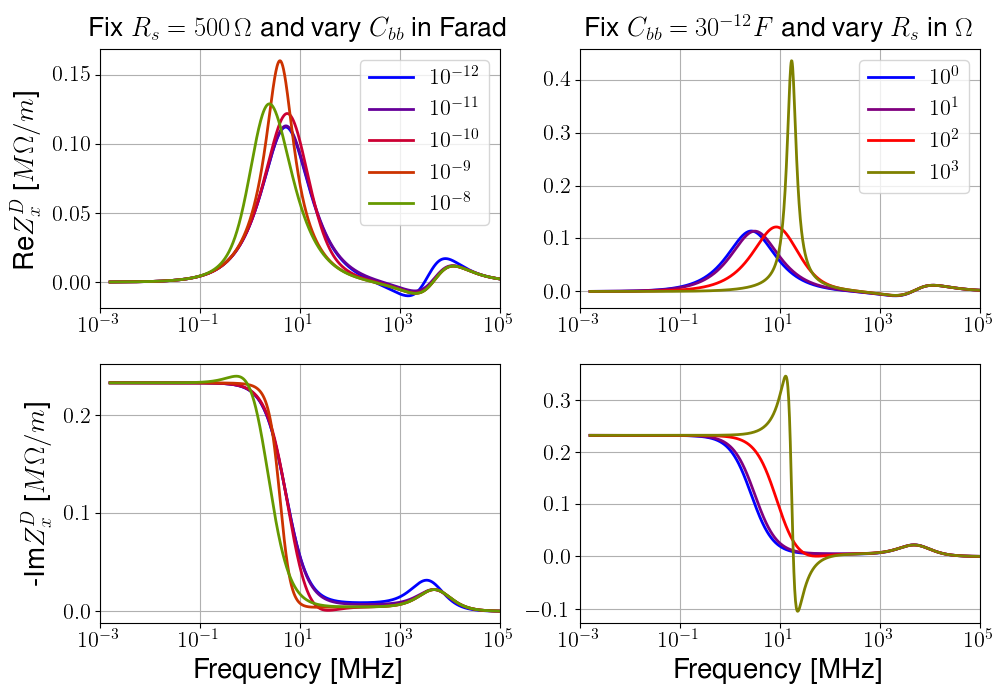
\includegraphics[width=0.8\textwidth]{kicker_coupled_flux.png}
        \caption{Coupled flux impedance of the dipole kicker magnet as function of the frequency for several values of capacitance (left) and resistance (right).}
        \label{fig:coupled_flux_impedance}
    \end{figure}
    shows the coupled flux horizontal impedance for some values of $C_{bb}$ and $R_s$, where the resonant behaviour created by the parallel association of the inductance $L_2$ with the capacitance $C_{bb}$ is evidenciated. In general, the variation of the parameters influence the positioning, intensity and width of the resonant peaks, all around a few \si{\mega\hertz}, but do not change the value of the imaginary impedance at lower frequencies. As will be shown below, the Titanium coating in the vacuum chamber shields the electromagnetic fields of the beam starting from approximately the frequency range of these peaks, thus, it is expected they will be attenuated. The low frequency impedance will not, and will influence the coupled-bunch motion, but not the incoherent tune shifts, because there is no quadrupolar impedance associated with this mechanism.

    Regarding the uncoupled flux, there are no formulas in the literature to estimate the impedance of an out--of--vacuum window--frame magnet as the one presented in Figure~\ref{fig:kicker_magnet}. There is, however, a model for an in--vacuum magnet developed by~\citeonline{Tsutsui2000} for the longitudinal impedance, which was extended to the transverse dipolar impedances by~\citeonline{Tsutsui2000a} and then to the quadrupolar impedance by \citeonline{Salvant2010a}. These formulas were derived by solving the \gls{maxeq} exactly for an ultra-relativistic beam, considering the geometry of Figure~\ref{fig:tsutsui_model},
    \begin{figure}
        \centering
        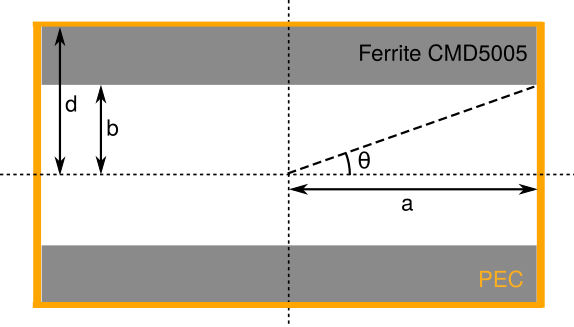
\includegraphics[width=0.6\textwidth]{tsutsui_model.png}
        \caption{Tsutsui model for the window--frame kicker magnet.}
        \label{fig:tsutsui_model}
    \end{figure}
    which is infinite in the longitudinal direction. Note that in this model the fraction of the fields generated by the beam that are inside the region defined by the angle $\theta$ directly interacts with a \gls{pec} material, which is an approximated model for the cooper plates of the real magnet, and the rest of the field directly see the ferrite, which is a lossy material. With the exception of the presence of the vacuum chamber, this is what happens in the real magnet, which makes this model a good approximation for the window--frame geometry.

    The ferrite that will be used in this magnet is the CMD5005~\cite{CeramicMagnets2017}. Its frequency dependent relative magnetic permeability was modeled by
    \begin{align}
        \mu_r(\omega) = 1 + \frac{\mu_i}{1+i\frac{\omega}{\omega_s}}
    \end{align}
    where $\mu_i$ is the initial permeability and $\omega_s$ is the saturation frequency of the material, which were obtained by fitting the datasheet curve. The values found agreed well with direct measurements made by~\citeonline{Hahn2002}.

    In order to estimate the effect of the vacuum chamber on the impedance, other models based on the round multi--layer formulas were analysed. The idea behind the formulation of these models is to try to account for limiting cases of the Tsutsui geometry in relation to the angle $\theta$, that defines the proportion of the fields that interact with a good conductor. Under these assumptions the models are:
    \begin{description}[align=left]
        \item[Worst case (W):] The beam only sees the ferrite. The layers of the round model in this case are composed by: Titanium, ceramic, air, ferrite and Copper;
        \item[Best case (B):] The beam only sees the good conductor: Titanium, ceramic, air and Copper;
        \item[No Coating (NC):] To show the effect of the Titanium coating, this layer was removed from the analysis of the worst case model: ceramic, ferrite, air and Copper.
    \end{description}

    Figure~\ref{fig:uncoupled_flux_impedance}
    \begin{figure}
        \centering
        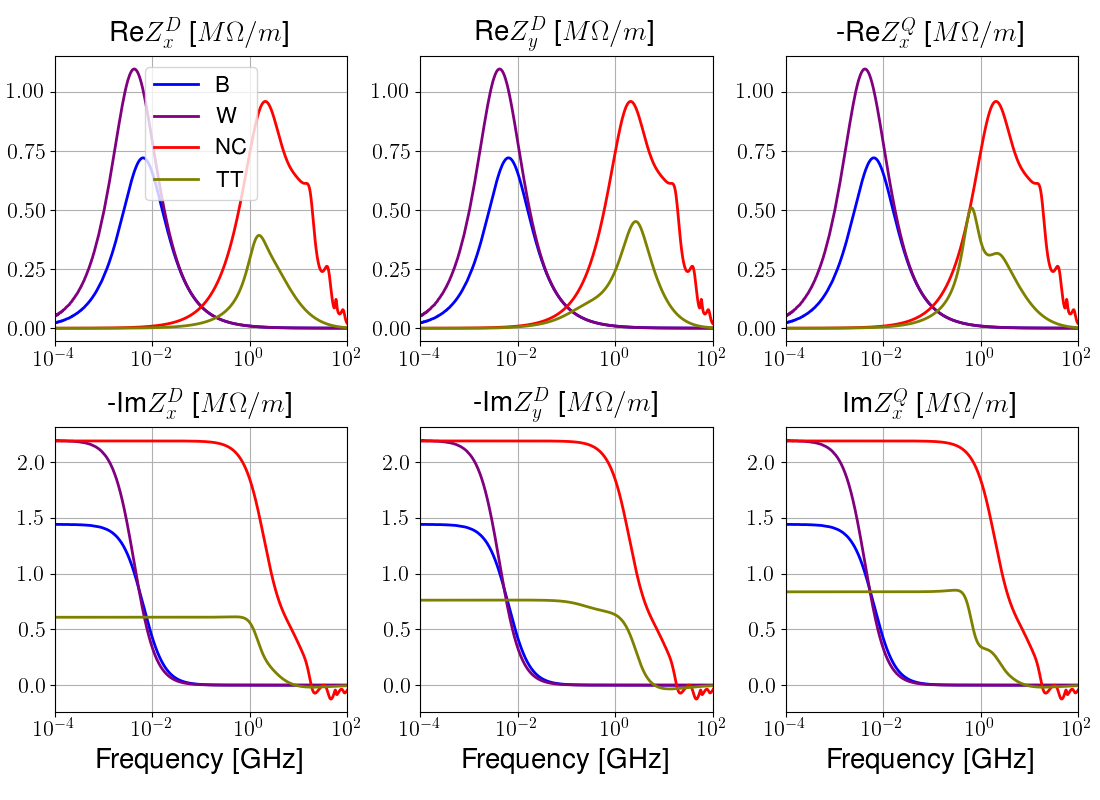
\includegraphics[width=\textwidth]{kicker_comp_models.png}
        \caption{Transverse impedances of the four models of kicker analysed.}
        \label{fig:uncoupled_flux_impedance}
    \end{figure}
    shows the transverse impedances of the four models analysed. The W curve matches the low frequency limit of the NC case, but at approximately \SI{1}{\mega\hertz} the coating starts to influence the impedance, damping all of them to very low values. Besides, the impedance predicted by the Tsutsui model (TT) is even lower than the B case, and that the relations between the three of them cannot be described by the constant \citeonline{Yokoya1993} factors, a property already pointed out by \citeonline{Salvant2010a}. Considering that this component have a stronger influence on the total budget due to the low frequency limit of the impedance, the model adopted for the transverse plane was the B case, multiplied by constant factors that matches its impedance to the tsutsui model. The values used were (0.42, 0.52, 0.58) for the dipolar horizontal, dipolar vertical and quadrupolar vertical impedances, respectively.

    For the longitudinal plane it is well--known from the works of \citeonline{Zotter1969} and \citeonline{Piwinski1977} that the coating influences the impedance at much lower frequencies than the skin depth of the metal. For this reason we varied the thickness of the Titanium layer in our simulations to check if it could be thinner than the nominal value. The results are shown in Figure~\ref{fig:kicker_comp_models_long},
    \begin{figure}
        \centering
        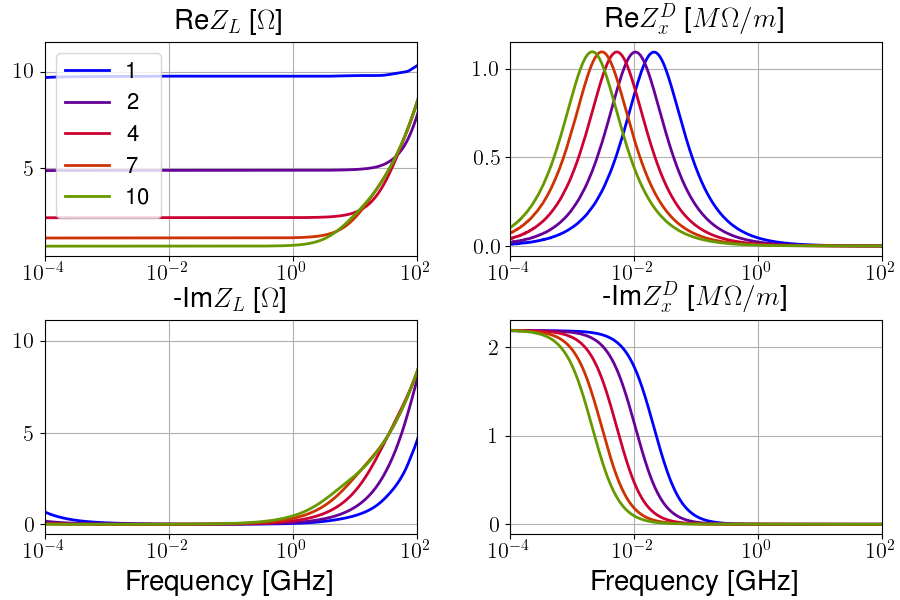
\includegraphics[width=\textwidth]{kicker_comp_models_long.png}
        \caption[Titanium coating thickness effect on impedance.]{Longitudinal (left) and dipolar horizontal (middle) impedances as function of the frequency for several values of coating thickness, in \si{\micro\meter}. The spectrum of a \SI{2.5}{\milli\meter} bunch is also shown (solid black) in the left to highlight the important part of the frequency spectrum, and the first horizontal betatron line (black dashed) is shown in the middle. In the right is shown the loss factor (above) and quadrupolar kick factor (below) as function of the bunch length for several values of coating thickness.}
        \label{fig:kicker_comp_models_long}
    \end{figure}
    where we note that indeed the coating is effective since very low frequencies, because of the difference from the result without coating. For almost all the relevant frequency range, the longitudinal impedance is constant, starting increasing only at large frequencies, because in this limit it is dominated by skin--depth effect on the Titanium and the standard resistive wall characteristics apply. However, note that the baseline of the impedance is almost inversely proportional to the thickness of the coating. This effect is seen in the behavior of the loss factor also shown in Figure~\ref{fig:kicker_comp_models_long}, which can be used to calculate the power density on the wall through equations~\eqref{eq:total_power},~\eqref{eq:power_density_circle}, and~\eqref{eq:power_density_flat}. Note that a reduction of the coating thickness to~\SI{4}{\micro\meter} would not impact the impedance and heating issues. In the transverse plane, the effect of the coating reduction is only to cause a linear shift on the frequency where the impedance is damped, which does not change its effect on the beam, as can be seen by the quadrupolar kick factor.

    Figure~\ref{fig:non_linear_kicker}
    \begin{figure}
        \centering
        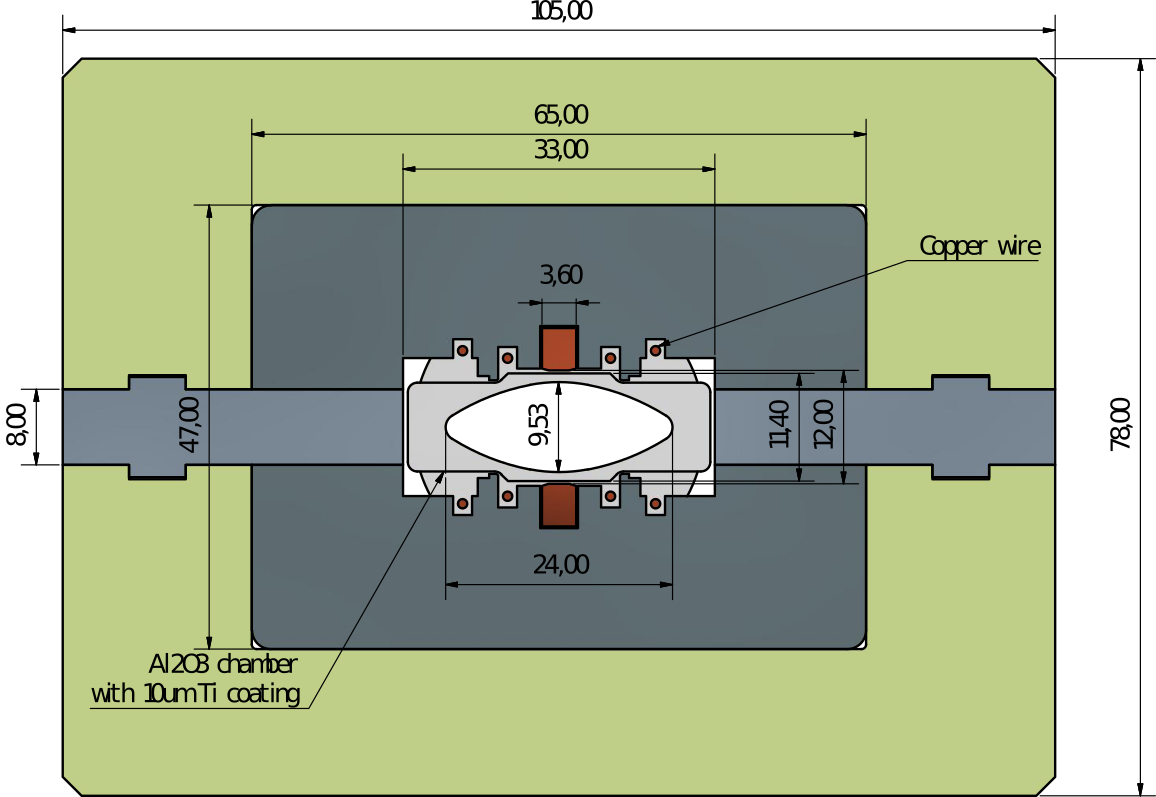
\includegraphics[width=0.6\textwidth]{MPP.png}
        \caption[Drawing of non--linear kicker magnet.]{Drawing of a deprecated version of the non--linear kicker that will be for injection in Sirius storage ring. The current version of the magnet does not have the copper blocks below and above the vacum chamber. The magnet core is made of FeSi.}
        \label{fig:non_linear_kicker}
    \end{figure}
    shows an old version of the non-linear kicker magnet that will be used in Sirius. Based on the study presented above, we defined the impedance of this kicker as a round multi--layer chamber with: vacuum, Titanium, ceramic, air, FeSi and Copper. Besides the substitution of the ferrite with the FeSi as the magnet core, this component does not have the parallel copper plates to induce a dipole kick on the beam, creating a much more complex transverse field dependence using copper wires displaced transversely.  Such property makes the use of the \citeauthor{Tsutsui2000} model unapropriate for this case, and instead of multiplying the resultant impedance of the round chamber by the same factors of the dipole kicker, we decided to use the \citeauthor{Laslett1963} coefficients, defined in equation~\eqref{eq:laslett_coefficients}. This magnet also does not have the coupled flux part of the impedance, because the external circuit does not couples with a beam close to the center of the magnet.

\section{Fast Correctors Chambers}

    The Fast orbit correctors of the Sirius storage ring will operate at an update rate of \SI{100}{\kilo\hertz} in the \gls{fofb}~\cite{Tavares2013}, requiring special vacuum chambers in order for such high frequency fields to penetrate. The solution adopted was to brase small and thin stainless steel chambers in the standard copper chamber of the ring. The reduced conductance, only \SI{1}{\mega\siemens}, of this material provides a skin depth of \SI{1.6}{\milli\meter} at \SI{100}{\kilo\hertz}, which is much larger than the thickness of the chamber, which is \SI{0.3}{\milli\meter}, and do not damp or distort significantly the external field of the magnet. The relevant parameters used for modeling of this type of chamber is presented in Table~\ref{tab:fast_correctors_chamber_parameters}.
    \begin{table}
        \centering
        \caption{Main parameters for the fast correctors impedance model.}
        \label{tab:fast_correctors_chamber_parameters}
        \begin{tabular}{lccc}
            \toprule
            Parameter            & Value      & Unit \\
            \midrule
            SS conductivity      & 1.3  & \si{\mega\siemens\per\meter}\\
            Chamber thickness    & 300  & \si{\micro\meter}\\
            Chamber radius       & 12   & \si{\milli\meter}\\
            Chamber length       & 100  & \si{\milli\meter}\\
            Number of elements   &  80  & \\
            \bottomrule
        \end{tabular}
    \end{table}

    The small length of these chambers, only~\SI{10}{\centi\meter}, raises a question on the validity of the infinitely long formulas of the multi--layer chambers used so far. This question is answered by~\citeonline{Shobuda2009}, who calculated the impedance of a finite resistive insert of finite thickness on an otherwise perfectly conducting and infinitely long round chamber. The authors conclude that even for an insert whose length is smaller than its radius, if the thickness is of the order of \SI{100}{\micro\meter}, the impedance is already equal to the infinitely long chamber counterpart. This result shows that the use of the multi--layer formulas employed so far for the other components are still valid for the fast correctors chambers.

\section{Undulators Chambers}\label{sec:undulators_chambers}

    For the first phase of operation of the Sirius light source it is planned the installation of seven \glspl{id} on the storage ring, with four different types of devices: two Delta-type undulators~\cite{Temnykh2008} and two \gls{apu}~\cite{Carr1991}. The design details as well as first experiences with the prototype measuments of the Sirius Delta undulator are described by~\citeonline{Vilela2017} and the information regarding the radiation parameters of such devices can be found elsewhere~\cite{Sirius2013}. All the \glspl{id} will be out of vacuum and their vacuum chamber will be made of copper and coated with \gls{neg}. Regarding the impedance issues, on the one hand this is good because it simplifies the design of the tapers, allowing further optimization of its parameters for impedance reduction, but on the other hand the resistive wall impedance will always be there, regardless of the existence or not of the additional damping provided by radiation emittion\footnote{One important remark is that both types of undulators that will be used in Sirius does not have the degree of freedom to change their gap, which means that when they are not being used there is no way to "turn off" their magnetic field. What is usually done is to change the phases among the~\citeonline{Halbach1985} cassets in such a way that the field lays down in the longitudinal direction, so the electron beam stops radiating.}.

    Table~\ref{tab:undulators_parameters}
    \begin{table}
        \centering
        \caption{Main parameters of the Undulators for their impedance modeling.}
        \label{tab:undulators_parameters}
        \begin{tabular}{lccccl}
            \toprule
            Parameter         & APU19     & APU20      & Delta21   & Delta52   &Unit\\
            \midrule
            Length            &  2.4      & 2.4        & 2.4       &  3.6      & \si{\meter} \\
            Quant. in Phase 1 &   1       &   1        &   2       &   3       & \\
            Quant. in Phase 2 &   2       &   3        &   6       &   6       & \\
            Straight type     & low--beta & high--beta & low--beta & low--beta & \\
            Full Magnetic Gap &   5       &   6.2      &   7.0     &  13.8     &  \si{\milli\meter} \\
            Chamber thickness &   0.10    &   0.10     &   0.80    &  1.00     & \si{\milli\meter} \\
            Hor. Beam Stay Clear&   24.0   &   24.0     &   8.2     &  11.2     & \si{\milli\meter} \\
            Vert. Beam Stay Clear&   4.8    &   6.0     &   5.0    &  8.0     & \si{\milli\meter} \\
            Transition factor ($t$)&  \mc{4}{c}{20}                             & \\
            \bottomrule
        \end{tabular}
    \end{table}
    shows the main impedance related parameters of each device type. These devices have two main source of impedance that will be modeled separately: one comes from the two tapers at both ends of the device and another from the resistive wall. The modeling of the tapers was performed with the whole collimator in the simulation, consideding perfectly conducting walls and linear transitions with factor\footnote{Here we recall the notation defined in subsection~\ref{ssec:tapered_transitions}.} $t$ equals to 20, which means the angle of the taper is \SI{2.86}{\degree} (\SI{50}{\milli\radian}), much lower than the rule of thumb of \SI{10}{\degree}. The \gls{apu} chambers were calculated with ECHOzR~\cite{Zagorodnov2015}, being modeled as flat collimators starting from a square chamber of sides equal to the radius of the real chamber and final gap equal to the Vertical \gls{bsc} defined in
    Table~\ref{tab:undulators_parameters}. The Delta--type undulators are a little more complicated to model, because their final chamber geometry is an ellipse with the major and minor axes given by the horizontal and vertical~\gls{bsc} presented in Table~\ref{tab:undulators_parameters}, which invalidates the consideration of a flat geometry, due to the non--negligible horizontal tapering. We delt with this problem by simulating a round transition with ECHOz2~\cite{Zagorodnov2005} and applying numerical factors given by~\citeonline[Figures 12a, 13 and 14]{Podobedov2007}, to the impedances. Even though their comparisons are valid for tapers with transverse sections composed by confocal ellipes, all the analytic formulas analysed in
    subsection~\ref{ssec:tapered_transitions} suggests that the parts of the tapers with lower gaps contributes more to the total impedance, which corroborates with this approach. The form factos used here were $(1,1.3,0.5,-0.4)$ for the longitudinal, vertical dipolar, horizontal dipolar and horizontal quadrupolar impedances, respectively.

    Figure~\ref{fig:undu_trans}
    \begin{figure}
        \centering
        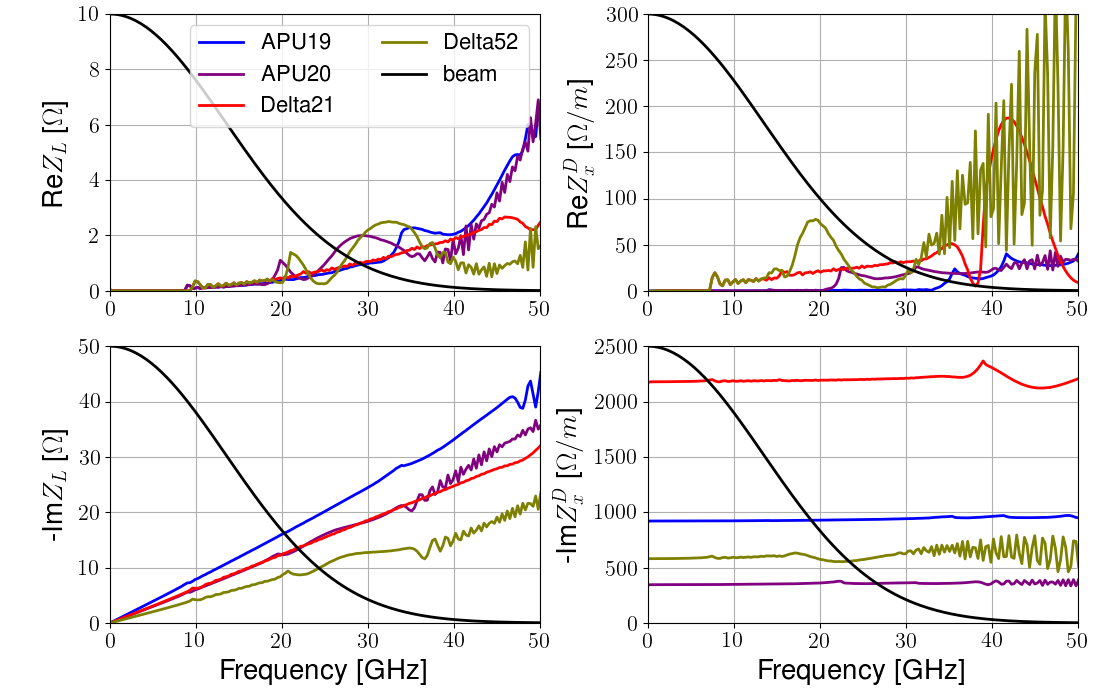
\includegraphics[width=\textwidth]{undu_trans.png}
        \caption{Geometric impedance from the tapered transitions of the undulators. Solid lines represent numerical calculations performed with ECHOz1 and ECHOz2 for the Delta undulator and with ECHOzR for the \gls{apu}. Dashed lines are the prediction by the analytic formulas studied in subsection~\ref{ssec:tapered_transitions}.}
        \label{fig:undu_trans}
    \end{figure}
    shows the impedances of the four \glspl{id} types before the application of the form factors on the Delta--type undulators. Also shown is the low frequency analytic expressions discussed in subsection~\ref{ssec:tapered_transitions}. Note that in general their quantitative agreement with the numerical simulations is not very good, but the qualitative comparisons among all the types of undulators, mainly the differences between the round and flat geometry, are well predicted by the theory. In the case of the longitudinal and horizontal impedances of flat geometries this quantitative difference between theory and numerical simulations could be explained by the fact that the second condition imposed on the limits of validity of the expressions ($h\ll w$) is not met in the cases studied here, because the tapers start with a square geometry.~\citeonline{Stupakov2007a} provides expressions for impedances for any ratio $h/w$, which consists on multiplying the integrands of equations~\eqref{eq:flat_transitions} by form factor functions that depends on $h(s)/w$. The paper has graphics that explicitly show the value of these form factors and, after a qualitative analysis, it can be concluded that they justify the differences observerd here. For the vertical dipolar impedance this scenario changes, because the analytic formula overestimates the impedance by a factor larger than four (they are above the upper limit of the graphic and are not shown), which is so large that even the form factors could not account for the difference observed. Maybe this disagreement, if our results are correct, comes from higher order terms in the taper angle that are not considered in the derivation of the analytic formulas.

    Another interesting aspect of the numerical calculated vertical dipolar impedance is the presence of the narrow--band trapped mode studied by~\citeonline{Blednykh2006} for the APU19. Considering that this mode depends strongly on the width of the chamber and the fact that the Sirius undulators were not desined yet, the complete effect of the this peak was not studied in details, being subject for future works. However, it was verified that it does not induce transverse coupled--bunch oscillations.

    Figure~\ref{fig:undu_wall}
    \begin{figure}
        \centering
        \begin{subfigure}[c]{0.65\textwidth}
            \centering
            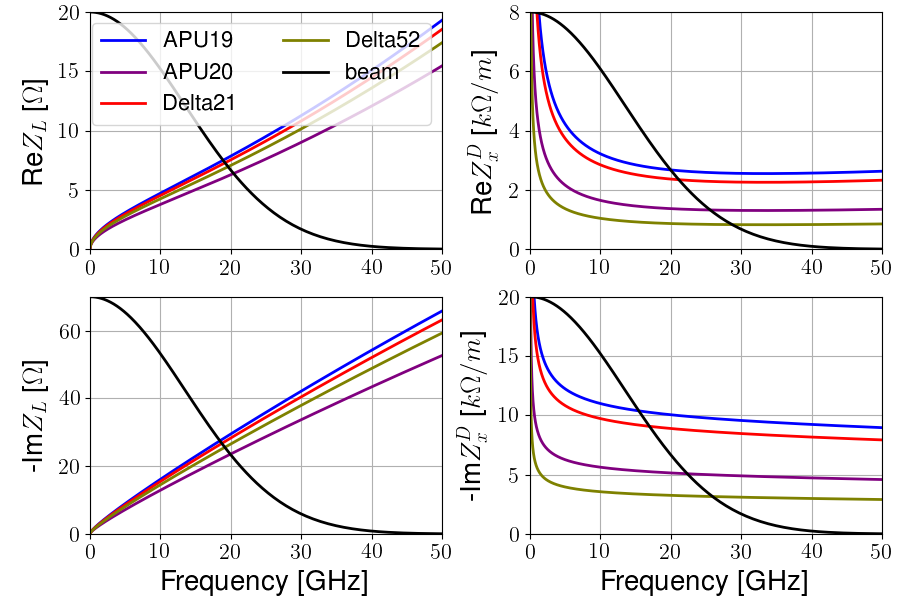
\includegraphics[width=\textwidth]{undu_wall.png}
            \caption{High frequency impedance}
            \label{fig:undu_wall_highfreq}
        \end{subfigure}
        \begin{subfigure}[c]{0.34\textwidth}
            \centering
            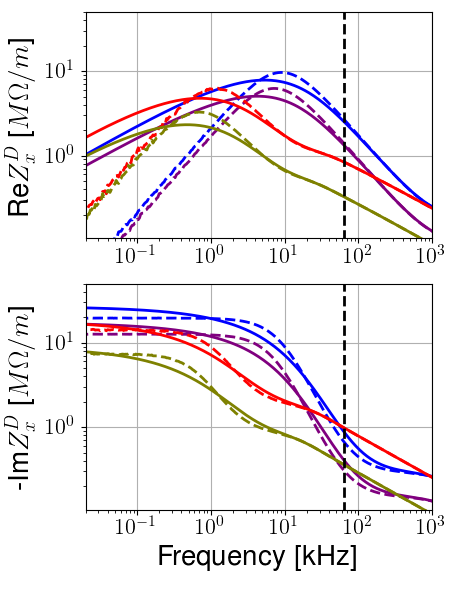
\includegraphics[width=\textwidth]{undu_wall_lowfreq.png}
            \caption{Low Frequency}
            \label{fig:undu_wall_lowfreq}
        \end{subfigure}
        \caption{Wall impedance of the four types of undulators planned for Sirius.}
        \label{fig:undu_wall}
    \end{figure}
    shows the vertical dipolar and longitudinal wall impedance of the four types of undulators. They were calculated using the code ImpedanceWake2D~\cite{Mounet2011} for flat multi--layer chambers. The layers used in the calculations were: \gls{neg}, Copper, air, high $\mu$--material. The last layer was added in an attempt to consider the effect of the magnet blocks of the \glspl{id} on the zero frequency impedance, which can be noted in Figure~\ref{fig:undu_wall_lowfreq}. This figure also show in dashed lines the results obtained with the calculation of the impedance using the round chamber formulas and posterior application of the \citeauthor{Yokoya1993} factors. Note that for the undulators with small gap (APU19, APU20 and Delta21), this method underestimate the impedance, because the sum of the electric and magnetic \citeauthor{Laslett1963} coefficients are larger than the factor for the quadrupolar impedance, but for the Delta52 both formulas agree because in this case only the electric coefficient contributes significantly and it is equal to $\pi^2/24$.
    ~\citeonline{Blednykh2016} created a more sofisticated model, where the authors considered that a fraction of the suface of the pole of the \glspl{id} was composed by the high $\mu$--materials and the other part by saturated ferromagnet blocks, with $\mu\approx1$. With this impedance they successfully explained the incoherent tune--shifts caused by these devices in LNLS2. Once the detailed model of the \glspl{id} are available we intent to improve these components impedance model in a similar way.

    The chamber heating is an important aspect to be considered in the design of the undulators, because it is difficult insert cooling systems in devices with such small gap, mainly in the Delta--type undulators, which have small appertures in both transverse directions. To estimate the power density for these devices we used the flat chamber approximation, described in equation~\eqref{eq:power_density_flat}. Even though the undulators chambers are not flat, the estimation of the peak density using this formula is a worst case scenario for the real value and, even in this case it was verified through heating simulations that the power deposited by the wake fields is not an issue.

\section{BC Chamber}\label{sec:bc_chamber}

    The BC magnet is the central dipole of the arch of the Sirius storage ring unit cell. It is a permanent magnet with longitudinal and transverse gradient and at its center there is a very thin slice that will reach a peak magnetic flux density of \SI{3.2}{\tesla} which will be used as source for 20 beamlines, providing radiation with critical energy of \SI{19.2}{\kilo\electronvolt}. In order to achieve this high flux density, the poles of central part must be very close to the beam, with a full gap of only \SI{10}{\milli\meter}.
    % Figure~\ref{fig:bc_magnet_with_twiss}
    % \begin{figure}
    %     \centering
    %     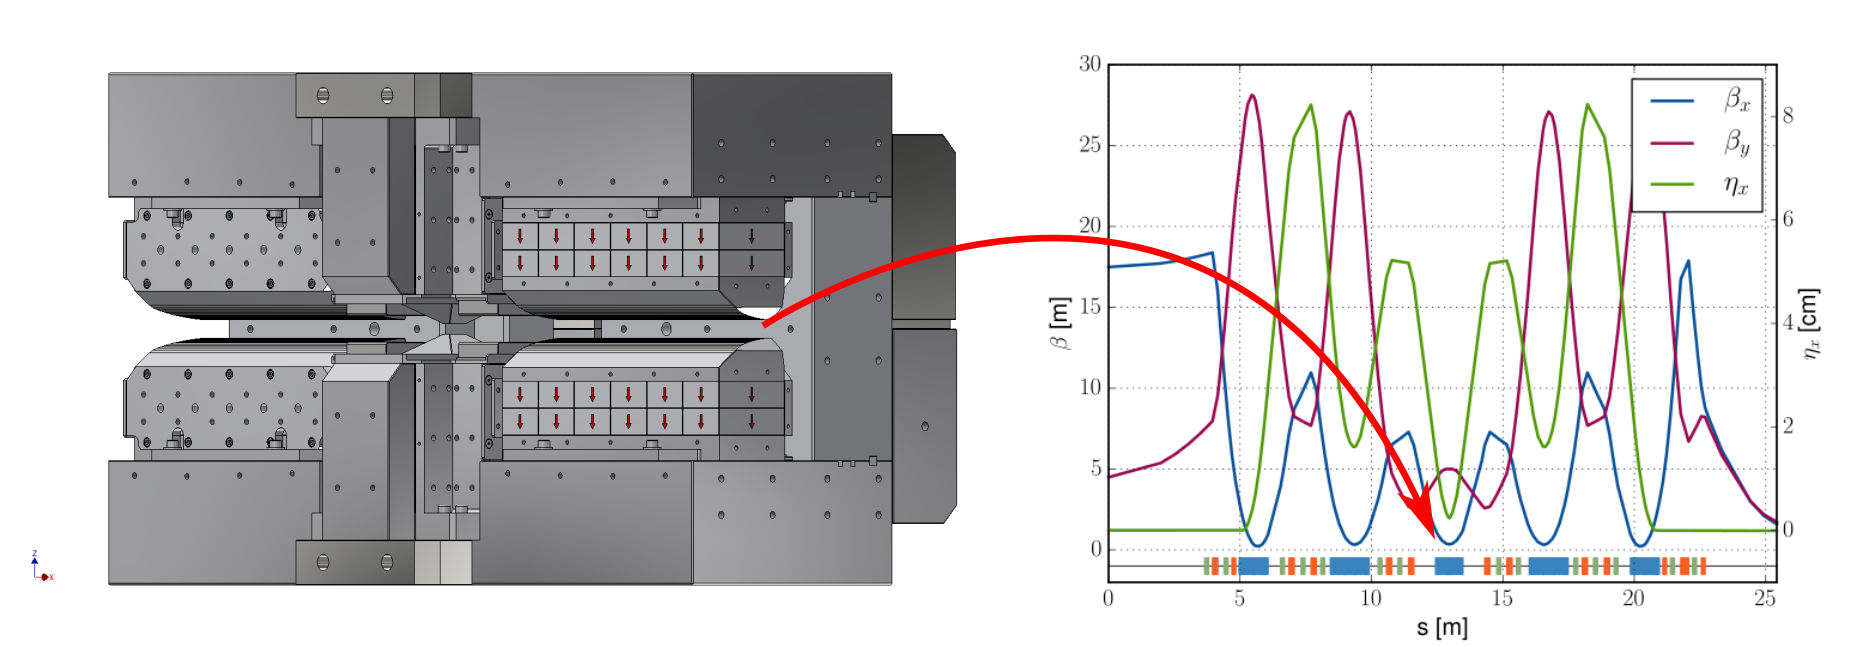
\includegraphics[width=\textwidth]{bc_magnet_with_twiss.png}
    %     \caption{Effect permeability wall impedance}
    %     \label{fig:bc_magnet_with_twiss}
    % \end{figure}
    % shows a drawing of this magnet and indicates the position where it will be installed in the ring.

    The initial proposal for the chamber of the central section of this magnet was a elliptical chamber with inner minor semi--axis equal to \SI{4}{\milli\meter} and major semi--axis equal to the radius of the standard chamber, \SI{12}{\milli\meter}, connected by a smooth tapered transition with transition factor equal to 15. Motivated by the analytic formulas predicted by the theory, discussed in subsection~\ref{ssec:tapered_transitions}, we also investigated the impedance of a round chamber with inner radius equal to the minor radius of the proposed elliptical chamber. For the impedance calculations, the elliptical chamber was approximated by a flat one and simulated using ECHOzR~\cite{Zagorodnov2015}, while the round chamber was simulated with ECHOz1 and ECHOz2~\cite{Zagorodnov2005}. It was known, however, that the round chamber did not meet the vacuum requirements, because the radiation generated by the upstream dipole would hit strongly the inner part of the transition in the positive (outward the storage ring center) horizontal direction, causing heating problems. For this reason, a chamber which satisfies the requirements, with a "keyhole" shape, as shown in Figure~\ref{fig:bc_keyhole_model},
    \begin{figure}
        \centering
        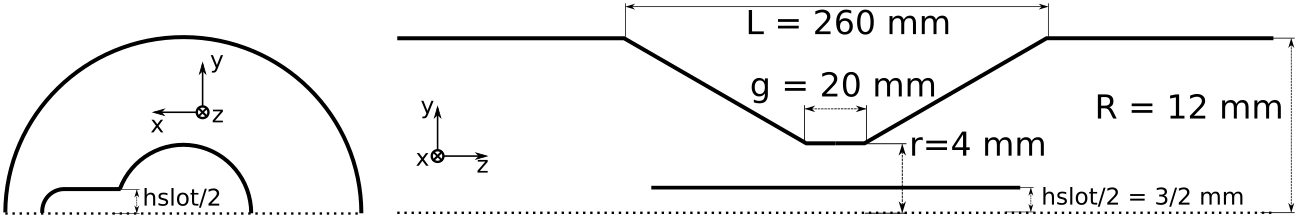
\includegraphics[width=0.8\textwidth]{bc_keyhole_model.png}
        \caption{Scheme of the keyhole--shaped chamber for the BC magnet.}
        \label{fig:bc_keyhole_model}
    \end{figure}
    was also proposed and its impedance simulated with GdfdL~\cite{Bruns2017}.

    Figure~\ref{fig:bc_zdy_comp}
    \begin{figure}
        \centering
        \begin{subfigure}[c]{0.48\textwidth}
            \centering
            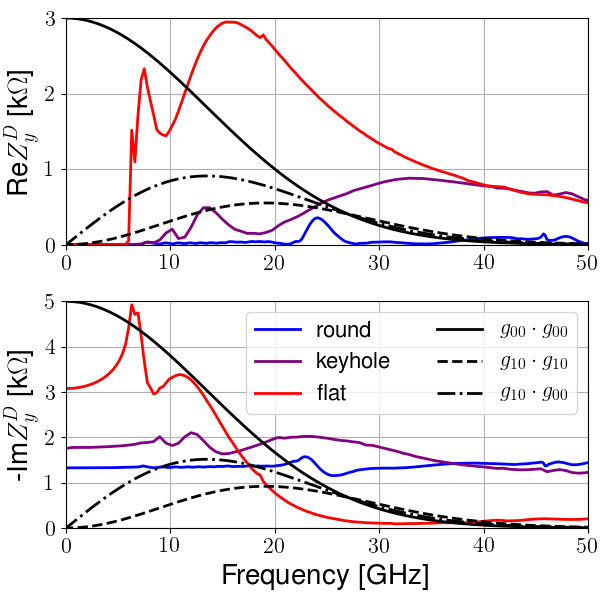
\includegraphics[width=\textwidth]{bc_Zdy_comp_spec.png}
            \caption{Vertical Impedance}
            \label{fig:bc_zdy_comp}
        \end{subfigure}\hfill
        \begin{subfigure}[c]{0.48\textwidth}
            \centering
            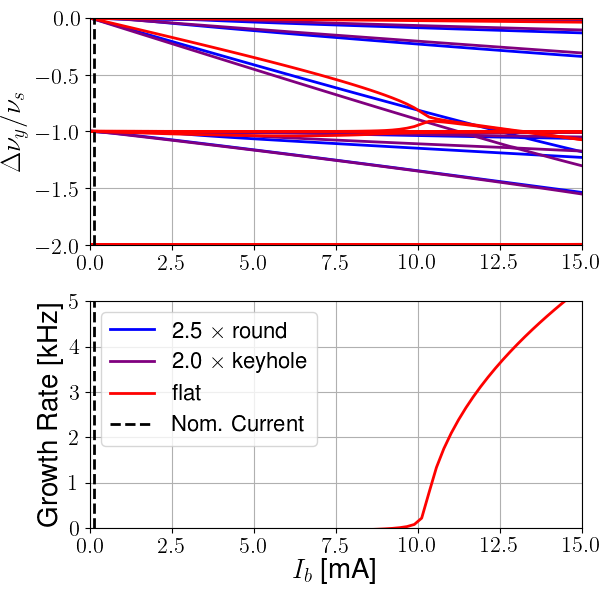
\includegraphics[width=\textwidth]{bc_tmci.png}
            \caption{Vertical \gls{tmci}}
            \label{fig:bc_tmci}
        \end{subfigure}
        \caption[Comparison of the vertical dipolar impedance among different models of BC chamber.]{Comparison of the impedance and its effect on the beam through simulations of mode--coupling instability for different models of impedance. For the \gls{tmci} a gaussian single bunch with \SI{2.5}{\milli\meter} \gls{rms} length was considered. The impedance used was that of the 20 components along the ring, multiplied by the averave betatron function at the magnet's position.}
        \label{fig:bc_comparisons}
    \end{figure}
     shows the comparison of the vertical dipolar impedance among the three models analysed. The theory predicts a higher low frequency inductive impedance for the flat chamber model and we note that this is indeed true. One interesting factor, however, is that the round chamber remains imaginary for all the frequency range analysed, its real part only emerges at frequencies larger than ~\SI{60}{\giga\hertz}, while the flat chamber has a very strong real part at low frequencies, which couples with the beam oscillation mode $g_{10}\cdot g_{00}$. From the theory of mode--coupling instability, discussed in subsection~\ref{ssec:transverse_mode_coupling}, we know that at zero chromaticity the imaginary part of the impedance causes tune--shifts of the coherent modes and bring them close to each other, in this case the modes~0~and~-1, represented in the figure by the spectra $g_{00}\cdot g_{00}$ and $g_{10}\cdot g_{10}$, respectively; but it is the real part of the impedance that couples them causing the intability. We can see this mathematically recalling that the mode--coupling matrix has the following form, when only the modes~0~and~-1 are considered
     \begin{align}\label{eq:bc_eigen_value}
         \frac{M}{N} \propto
         \begin{pmatrix} I_1 -\frac1N & R_1 \\ -R_1 & I_0 \end{pmatrix}
         \Rightarrow
         \frac{\lambda_{1,2}}{N} \propto \frac{I_0 + I_1 -\frac1N}{2} \pm \frac12\sqrt{\fof{I_1-\frac1N - I_0}^2 - 4R_1^2}
     \end{align}
     where $N$ is the number of particles in the bunch,
     \begin{subequations}
         \begin{align}
             I_i &= \udefint{\omega}{\imag{Z^D_y}g_{i0}g_{i0}} \\
             R_1 &= \udefint{\omega}{\real{Z^D_y}g_{10}g_{00}},
         \end{align}
     \end{subequations}
     and $g_{ml}$ is given by equation~\eqref{eq:gaussian_oscillation_modes}. Henceforth, it is clear from the eigen--value expression in equation~\eqref{eq:bc_eigen_value} that the instability can only happen if the real part of the impedance is strong enough to couple with beam in such a way that
     \begin{align}
         2|R_1| \ge \left| I_1 - \frac1N - I_0 \right|.
     \end{align}
     Note that when the number of particles in the bunch is small, the \gls{rhs} of the inequality above is very large and when $N\to\infty$ it tends to $I_1-I_0$. If $R_1$ is not larger than this difference, the modes simply cross each other. Note that some mechanism similar to the one explained above is happening in Figure~\ref{fig:bc_tmci} for the round and keyhole chambers, where even after being multiplied by a factor of 2.5 and 2.0, respectively, to match the tune--shifts, their real impedances is not strong enough to create the instability.

     Figure~\ref{fig:bc_comp_spec}
     \begin{figure}
         \centering
         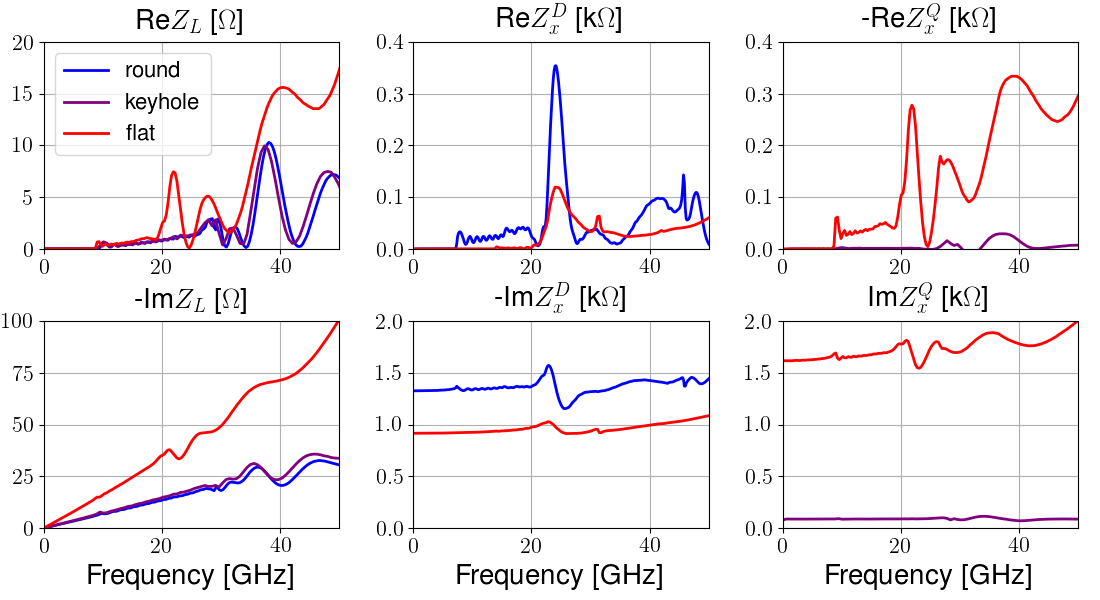
\includegraphics[width=\textwidth]{bc_comp_spec.png}
         \caption[Comparison of impedances of different models of BC chamber.]{Longitudinal (left), dipolar horizontal (center) and quadrupolar horizontal (right) impedances for the three models of BC chamber considered. The dipolar horizontal impedance of the keyhole chamber was not calculated yet and the round chamber does no have a quadrupolar impedance.}
         \label{fig:bc_comp_spec}
     \end{figure}
     shows the other impedances for the three models. Note that the imaginary part of the longitudinal impedance of the keyhole and round models are smaller than the one of the flat chamber by a factor of approximately 2, which is accordance with the theory predictions, and the quadrupolar impedance introduced by keyhole is negligible. The horizontal dipolar impedance was not calculated for this model yet, but a calculation was performed for a keyhole geometry with the $hslot$, defined in Figure~\ref{fig:bc_keyhole_model}, equals to \SI{2}{\milli\meter} and it was similar to the transverse impedance of the round model.

\section{\Glsentryfull{csr}}\label{sec:csr_impedance}

    The radiation emitted by one particle can influence other particles in the bunch in a similar way as the wake fields and, for this reason, is treated with the same formalism of impedances and wake functions discussed so far. Such mechanism is often refered to as \gls{csr} because its net effect is only relevant for wavelengths of the same order or larger than the bunch length, according to~\citeonline{Nagaoka2014}. The wake function of a source particle moving in circular trajectory in free--space over a witness particle in this same trajectory was calculated by~\citeonline{Derbenev1995} and is given by:
    \begin{align}\label{eq:csr_wake_free_space}
        \frac{W'_0(z)}{L} =
        \begin{dcases}
            -\frac{Z_0 c}{2 \pi 3^{4/3}} \frac{1}{\rho^{2/3}(-z)^{4/3}} & z<0\\
            0 & z>0
        \end{dcases},
    \end{align}
    where $\rho$ is the radius of curvature of the trajectory, $L=2\pi\rho$ is the total length of the circle and, contrary to other wakes, it only affects particles ahead of the source particle. Notice that this formula not only diverges at the origin as it predicts energy gain for all ranges of interaction. This happens because this equation is only the tail of a very short--range and intense wake. This wake starts at $W'_0(0^-)\approx\gamma^4/\rho^2$, crosses zero at $-z\approx 2\rho / 9\gamma^2$ and soon after that assumes the value of the asymptotic behavior described by the equation above\footnote{Figure 2 of  \citeonline{Murphy1997} has a graphic of this function.}. A fast calculation shows that the short--range scales of the complete wake ($\rho/\gamma^2 \approx $\SI{500}{\nano\meter} for Sirius) are much smaller than any characteristic length important for the stability analysis in Sirius, which justifies the use of equation~\eqref{eq:csr_wake_free_space}.

    \citeonline{Murphy1997} calculated the wake function of the same trajectory described above, but instead of considering the particles were in free space, the authors included two infinite parallel plates equally spaced from the particles trajectory. The asymptotic form of the wake they obtained has, in addition to the term of equation~\eqref{eq:csr_wake_free_space}, a contribution from the radiation of the image charges on the plates, given by
    \begin{align}\label{eq:csr_wake_shielding}
        \frac{W'_1(z)}{L} = -\frac{Z_0 c}{4\pi}\frac{1}{2\pi h^2} G\fof{\frac{\rho^{1/2}}{h^{3/2}}z},
    \end{align}
    where $h$ is the distance of any one of the plates to the beam trajectory and the function $G$ is given by
    \begin{align}
        G(x) = 8\pi\sum_{k=1}^\infty \frac{(-1)^{k+1}}{k^2}\frac{Y_k(x)\fof{3-Y_k(x)}}{\fof{1+Y_k(x)}^3},
    \end{align}
    with $Y_k(x)$ being one of the roots of the equation
    \begin{align}
        Y_k - \frac{3x}{k^{3/2}}Y_k^{1/4} - 3 = 0.
    \end{align}
    According to~\citeonline{Bane2010} from the four roots of the equation above, two are complex and two are real and we are interested in the one that gives the larger value for $Y_k(x)$ when $x<0$, the smallest for $x>0$ and when $x=0$ the two real roots are equal to 3. Figure~\ref{fig:csr_ykx}
    \begin{figure}
        \centering
        \begin{subfigure}[c]{0.48\textwidth}
            \centering
            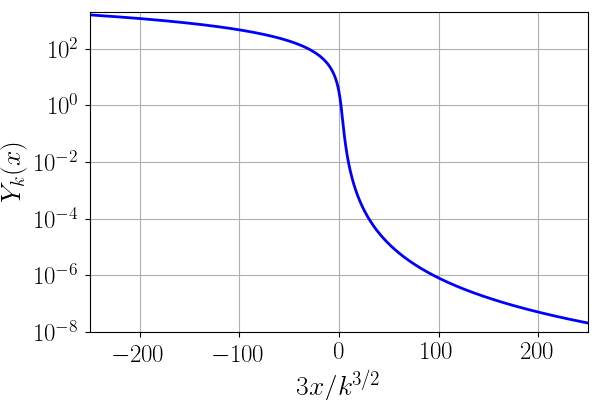
\includegraphics[width=\textwidth]{csr_ykx.png}
            \caption{}
            \label{fig:csr_ykx}
        \end{subfigure}\hfill
        \begin{subfigure}[c]{0.48\textwidth}
            \centering
            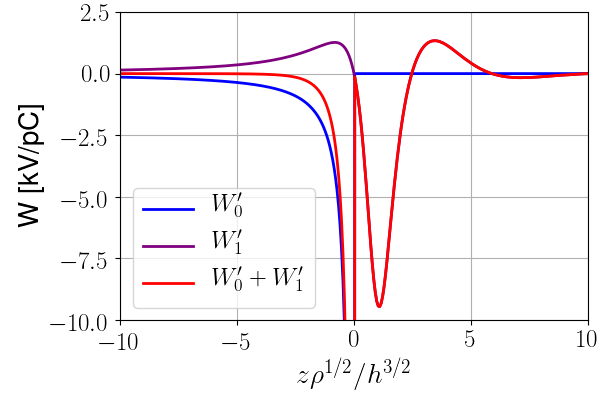
\includegraphics[width=\textwidth]{csr_shielding.png}
            \caption{}
            \label{fig:csr_shielding}
        \end{subfigure}
        \caption{(a) shows the behavior of the the function $Y_k(x)$ as function of $3x/k^{3/2}$ evidenciating its smooth dependency. (b) shows the sum of the two terms of the \gls{csr} impedance: the free--space contribution, $W'_0$ and the shielding term, $W'_1$, where it becomes clear the cancelation of the long tail at positions ahead of the emitting particle ($z$ negative).}
    \end{figure}
    shows $Y_k(x)$ as function of the term $3x/k^{3/2}$, where we note a smooth and well behaved dependency, which guarantees a fast convergence of the infinite series that defines $G$, being necessary to compute only the first 25 to 30 terms in almost all practical cases. Figure~\ref{fig:csr_shielding} shows the effect of the plates on the total wake, where we can note that, contrary to the free--space term, it is non--zero behind the source particle and that its contribution in the portion ahead is to cancel the long tail of the free--space wake, working as a shield for low frequency terms.

    The \gls{csr} impedance with and without shielding is known for a long time, see for example the work of~\citeonline{Faltens1972}. The free-space impedance, corresponding to the wake given in equation~\eqref{eq:csr_wake_free_space} is given by~\cite[Eq. 18]{Nagaoka2014}
    \begin{align}\label{eq:csr_imp_free_space}
        \frac{Z(\omega)}{L} = \frac{Z_0}{2\pi}
                            \frac{\Gamma\fof{2/3}}{3^{1/3}}
                            \exp\fof{\frac{i\pi}{6}}
                            \fof{\frac{\omega}{c\rho^2}}^{1/3}.
    \end{align}
    Calculations of the impedance of the shielded configuration with the parallel plates can be found in ~\citeonline{Warnock1990} and~\citeonline{Murphy1997}. However, recently~\citeonline{Cai2011} presented an approximated result that he built based on the exact equations given by~\citeauthor{Warnock1990} which is easy to calculate numerically and simply describes the impedance in terms of scaled results
    \def \Ai {\text{Ai}}
    \def \Bi {\text{Bi}}
    \def \Ci {\text{Ci}}
    \begin{align}\label{eq:csr_imp_shielding}
        \frac{\rho}{h} \frac{Z(n)}{n} = 16 Z_0 u_0
                        \sum_{p=0}^\infty \fof{\Ai'(u_p)\Ci'(u_p) +
                                            u_p\Ai(u_p)\Ci(u_p)},
    \end{align}
    where $n=\omega\rho/c$, $\Ai$ and $\Bi$ are the Airy functions~\cite{wiki2017c} and the prime denotes their derivatives, $\Ci = \Ai - i\Bi$ and the variable $u_p$ is given by
    \begin{align}
        u_p = \frac{\pi^2(2p+1)^2}{2^{2/3}}\fof{n\fof{\frac{2h}{\rho}}^{3/2}}^{-4/3}.
    \end{align}

    \def \Scsr {\fof{S_\text{csr}}_\text{th}}
    Using the parallel plates model for the~\gls{csr} impedance~\citeonline{Bane2010} calculated the threshold for the microwave instability as function of the plates separations using a \gls{vfp} equation solver developed by~\citeonline{Warnock2000} and showed that the~\gls{csr} induced instability depends on only two scaled variables: the threshold strength, $\Scsr$, and the shielding parameter, $\Pi$, given by
    \begin{align}\label{eq:csr_shielding_strength}
        \Scsr = I\frac{\rho^{1/3}}{\sigma_{z,0}^{4/3}}, & &  \Pi = \sigma_{z,0}\frac{\rho^{1/2}}{h^{3/2}}
    \end{align}
    where $\sigma_{z,0}$ is the bunch length at zero current and $I$ is a normalized bunch current (with unit of \si{\meter} in the \gls{si}) given by
    \begin{align}\label{eq:normalized_current}
        I = \frac{Z_0c}{4\pi}\frac{I_0T_0}{2\pi\nu_{s,0}\fof{E_0/e}\sigma_{\delta,0}},
    \end{align}
    where $N_b$ is the number of particles in the bunch, $\nu_{s,0}$ is the zero--current synchrotron tune and $\sigma_{\delta,0}$ is the zero--current energy spread. Figure~\ref{fig:csr_bane_graphic_modified}
    \begin{figure}
        \centering
        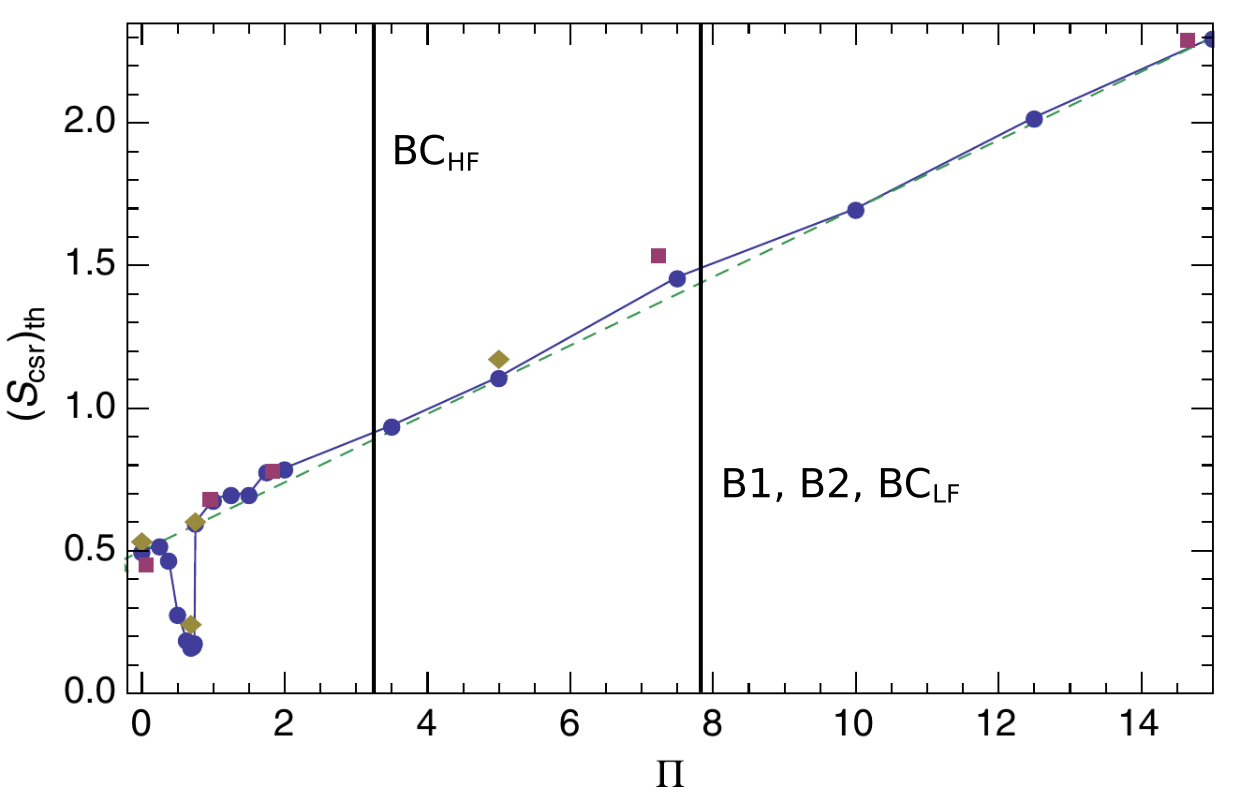
\includegraphics[width=0.7\textwidth]{csr_bane_graphic_modified.png}
        \caption[CSR driven longitudinal instability (adapted from~\citeonline{Bane2010}).]{Plot adapted from~\citeonline{Bane2010}: \gls{csr} threshold strengh, $\Scsr$, as function of the shielding parameter, $\Pi$. Blue dots: simulations with the \gls{vfp} solver; red squares: results of the linearized Vlasov equation (does not include damping); olive diamonds: results with a damping factor two times larger; dashed line: the scaling $\Scsr = 0.5 + 0.12\Pi$; black line: shielding parameters for the low field dipoles of Sirius, B1, B2 and the low field part of the BC magnet (BC$_\text{LF}$). The shielding for the high field part of this same magnet (BC$_\text{HF}$) is larger than the maximum value showed.}
        \label{fig:csr_bane_graphic_modified}
    \end{figure}
    shows their main results with the addition of one line indicating the shielding parameter for Sirius the low field dipoles, where one can note that if the whole ring were composed of only this type of dipole the threshold would be $\Scsr=0.90$, which converted to bunch current is \SI{0.9}{\milli\ampere}.

    Note that for most of the shielding range simulated, the threshold follows a simple dependency given by the line
    \begin{align}\label{eq:csr_scaling_instability}
        \Scsr = 0.5 + 0.12\Pi.
    \end{align}
    Despite of the simple model for the impedance used in these calculations, several expirements confirmed the instability predictions above, for example the one performed at the Metrology Light Source explained by~\citeonline{Ries2012} and the more recent results from ANKA, described in~\citeonline{Brosi2016}. However, the threshold calculated this way does not take into account the effect of other impedances, requiring a more specific study.

    Inspired by these good agreements between theory and measuments we decided to create an initial model for the \gls{csr} impedance based on this parallel plate approximation. Table~\ref{tab:csr_main_parameters} shows the main parameters used for modeling the impedances and wakes for the case of the Sirius storage ring.
    \begin{table}
        \centering
        \caption{Main parameters used for modeling the \gls{csr} impedance and effective wake function}
        \label{tab:csr_main_parameters}
        \begin{tabular}{lccc}
            \toprule
            Parameter              & B1, B2, BC$_\text{LF}$ & BC$_\text{HF}$ & Unit \\
            \midrule
            Bending radius         & 17.2             &  3.1  &\si{\meter}\\
            Magnet length          & 0.8/1.2/0.4      &  0.06 &\si{\meter}\\
            Total deflection angle & 337.6            &  22.4 &\si{\degree}\\
            Vacuum chamber radius  & 12               &  4    &\si{\milli\meter}\\
            Shielding parameter    & 7.8              &  17.5 & \\
            Threshold current      & 0.9              &  2.9  & \si{\milli\ampere}\\
            \bottomrule
        \end{tabular}
    \end{table}
    The impedance was directly calculated from equation~\eqref{eq:csr_imp_shielding}, but the method to obtain the wake was more involving. Instead of the wake-function of the point charge, we convolved the the expressions of equations~\eqref{eq:csr_wake_free_space} and~\eqref{eq:csr_wake_shielding} with a small gaussian beam of $\sigma = 5~$\si{\micro\meter} to avoid the divergence of the free--space wake and used this effective wake function as input for tracking simulations. The convolution with the shielded contribution was done in the standard numeric way, but the one with the free--space part of the wake was performed following the trick described by~\citeonline{Nagaoka2014}
    \begin{align}\label{eq:csr_convolution}
        V_0(z) = \infint{x}{W'_0(x)\lambda(z-x)} = -\infint{x}{W_0(x)\lambda'(z-x)},
    \end{align}
    where the divergence of the first integral of the equation above is neglected and the remainder is integrable. This procedure is justified by the fact that what causes this divergence is the approximated expression of the wake; the real physical one is finite. This is just a clever way to remain using the useful approximation for the free-space wake which does not depend on the particle's energy. The explicit expressions for the integrands are
    \begin{align}
        \frac{W_0(z)}{L} =
        \begin{dcases}
            \frac{-Z_0 c}{2 \pi 3^{1/3}} \frac{1}{\rho^{2/3}(-z)^{1/3}} & z<0\\
            0 & z>0
        \end{dcases}& &\text{and} &&\lambda'(z) = -\frac{z}{\sqrt{2\pi}\sigma^3}\exp\fof{-\frac{z^2}{2\sigma^2}}.
    \end{align}
    Note that $W_0(z)$ also diverges at the origin, but slower, in such a way that the convolution can be carried out numerically or analytically. The analytic result was obtained with Wolfram Mathematica~\cite{WolframResearchInc.2016} and it reads
    \begin{align}\nonumber
        \frac{V_0(z)}{L} =
        \frac{Z_0 c}{4\pi^{3/2}(3\sqrt{2}\rho^2\sigma^{10})^{1/3}}
        &\left\{
            \sqrt{2}\Gamma\fof{\frac56}
            \fof{
                \sigma^2\pFq{-\frac13}{\frac12}{-\frac{z^2}{2\sigma^2}} -
                      z^2\pFq{\frac23}{\frac32}{-\frac{z^2}{2\sigma^2}}
                }\right. \\\nonumber
        &   \left.+ z\sigma\Gamma\fof{\frac43}
            \fof{
                 3\pFq{\frac16}{\frac12}{-\frac{z^2}{2\sigma^2}} -
                 2\pFq{\frac16}{\frac32}{-\frac{z^2}{2\sigma^2}}}\right\},
    \end{align}
    where ${}_1\!\text{F}_1$ is the confluent hypergeometric function~\cite{wiki2017b}.
    Figure~\ref{fig:csr_wake}
    \begin{figure}
        \centering
        \begin{subfigure}[c]{0.48\textwidth}
            \centering
            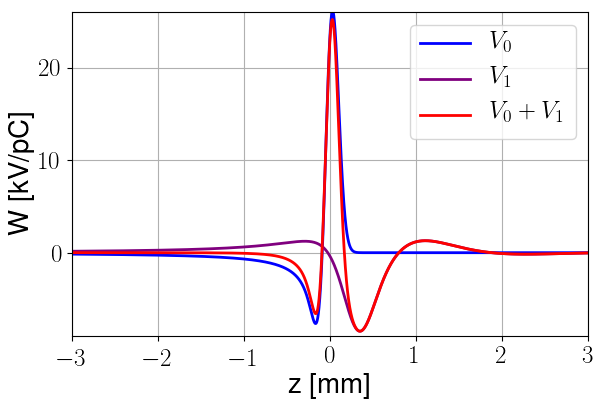
\includegraphics[width=\textwidth]{csr_wake.png}
            \caption{Effective wake functions.}
            \label{fig:csr_wake}
        \end{subfigure}\hfill
        \begin{subfigure}[c]{0.48\textwidth}
            \centering
            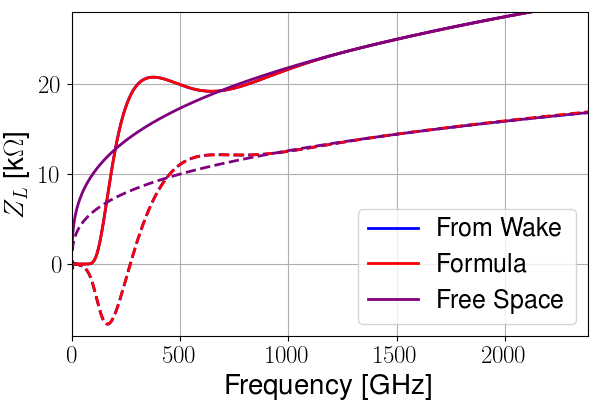
\includegraphics[width=\textwidth]{csr_impedance.png}
            \caption{Impedances.}
            \label{fig:csr_impedance}
        \end{subfigure}
        \caption{\gls{csr} effective wake functions and impedances calculated using the parameters of the Sirius low field dipoles.}
    \end{figure}
    shows the two components of the wake and their sum, while Figure~\ref{fig:csr_impedance} shows the impedance calculated via the Inverse Fourier Transform and posterior deconvolution of equation~\eqref{eq:csr_convolution}, compared with the calculation using equation~\eqref{eq:csr_imp_shielding} and the free-space impedance~\eqref{eq:csr_imp_free_space}. Note the very good agreement between the two methods of calculating the impedance, which validates the trick for calculation of the effective wake function.
    Besides, note that the shielding virtually eliminates the resistive part of the impedance up to approximately~\SI{100}{\giga\hertz} and changes the sign of the imaginary part from positive, which is generally refered as capacitive in the accelerators comunity, to negative, often called inductive. However, the impedance in this range of frequencies may depend very strongly on the parameters of the vacuum chamber geometry, for example,~\citeonline{Warnock1990a} calculated the radiation impedance for a beam in a circular smooth toroidal chamber with rectangular cross sections and found that the impedance at low frequencies would also be imaginary, but capacitive. The importance of this impedance to the budget is not in the frequency region of the stationary beam spectrum, but the very strong impedance at high frequencies, because the instability arises when modulations in the beam distribution starts radiating coherently, as explained by~\citeonline{Stupakov2002}.

    Figure~\ref{fig:csr_total_impedance}
    \begin{figure}
        \centering
        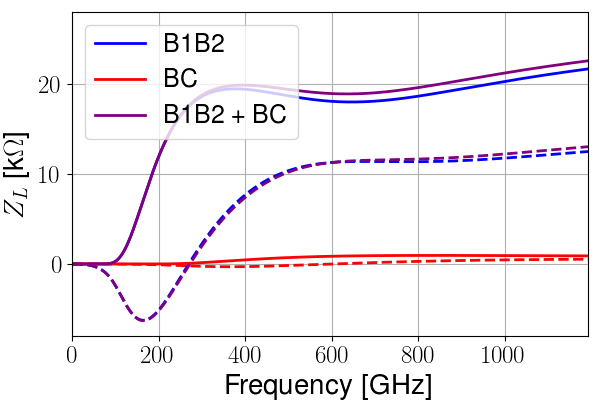
\includegraphics[width=0.48\textwidth]{csr_imp_comp_b1b2_bc}\hfill
        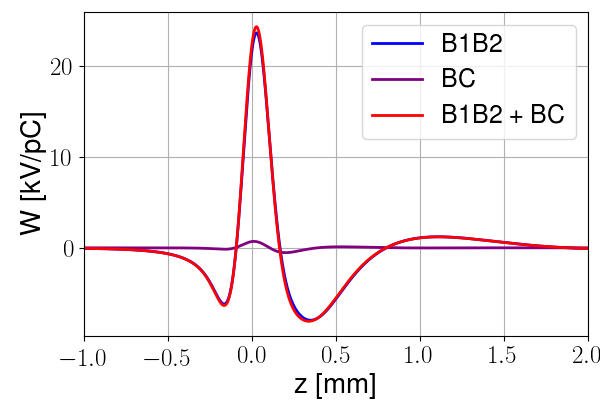
\includegraphics[width=0.48\textwidth]{csr_wake_comp_b1b2_bc}
        \caption{Total \gls{csr} impedance model for Sirius, considering the two types of dipoles.}
        \label{fig:csr_total_impedance}
    \end{figure}
    shows the total impedance considered for Sirius. The contribution from both types of dipoles was calculated considering their total length along the ring. Notice that the strong shielding factor of the BC magnet helps reducing the total impedance, in such a way that the threshold predicted by equation~\eqref{eq:csr_scaling_instability} rises to \SI{1}{\milli\ampere}.

    As a final remark we reinforce that this is only the initial model for the impedance, future works could consider the analytic results obtained by~\citeonline{Stupakov2016}, where the authors developed a general method to calculate the impedance for any planar trajectory in free space, and with the parallel plates shielding, and applied it to some practical cases, including the case of a finite dipole followed by a straight section. Another possibility is to use the results from~\citeonline{Stupakov2009b}, where the authors used a method developed in a previous paper~\cite{Stupakov2003} to calculate the impedance of a finite dipole in a rectangular chamber. Besides, numerical solvers such as the one developed and described by~\citeonline{Zhou2012} based on a method for solving the parabolic equation by~\citeonline{Agoh2004} could be employed.


\chapter{Impedance Budget}\label{cap:impedance_budget}

    The main aspects of the whole impedance budget of the Sirius storage ring will be discussed in this chapter. Besides the components whose modeling were analyzed in Chapter~\ref{cap:impedance_modeling}, several others are also included. Table~\ref{tab:impedance_budget}
    \begin{sidewaystable}
        \centering
        \caption{Sirius storage ring impedance budget for phase 1. RW stands for Resistive wall and Trans for transitions.}
        \label{tab:impedance_budget}
        \resizebox{0.78\textwidth}{!}{
        \begin{tabular}{l d{0} d{-1} d{-1} d{-1} d{-1} d{-1} c d{-1} d{-1} d{-1} d{-1}}
            \toprule
                          & & & & \mc{3}{c}{Multi bunch {@} \SI{100}{\milli\ampere}} & & \mc{4}{c}{Single bunch [kV/pC]} \\\cmidrule{5-7}\cmidrule{9-12}
                          & \mc{1}{c}{Q} &\mc{1}{c}{$\beta_x$ [m]} & \mc{1}{c}{$\beta_y$ [m]}
                          & \mc{1}{c}{$\kappa_{Loss}$ [V/pC]} & \mc{1}{c}{$Z_L/n|_{eff}$ [$m\Omega$]} & \mc{1}{c}{$P_{Loss}$ [W]} &
                          & \mc{1}{c}{$\beta_x\kappa_x^D$} & \mc{1}{c}{$\beta_y\kappa_y^D$} & \mc{1}{c}{$\beta_x\kappa_x^Q$} & \mc{1}{c}{$\beta_y\kappa_y^Q$} \\
            \midrule
            Pipe RW        &  1   &  6.0   &  11.0   &   6.80 &  -41.43 &  136.11 & &  -10.11 &  -18.52 &   0.02 &  -0.30 \\
            Delta21 RW     &  2   &  2.2   &  2.2    &   0.31 &   -1.91 &    6.27 & &   -1.62 &   -3.22 &   1.66 &  -1.66 \\
            Delta52 RW     &  3   &  2.6   &  2.6    &   0.44 &   -2.68 &    8.82 & &   -1.05 &   -2.09 &   1.09 &  -1.09 \\
            APU19 RW       &  1   &  2.2   &  2.2    &   0.16 &   -0.99 &    3.27 & &   -0.91 &   -1.82 &   0.95 &  -0.95 \\
            APU20 RW       &  1   &  17.8  &  5.0    &   0.13 &   -0.79 &    2.61 & &   -3.78 &   -2.11 &   3.95 &  -1.11 \\
            BC RW          &  20  &  0.4   &  5.2    &   0.05 &   -0.30 &    0.98 & &   -0.04 &   -0.57 &        &        \\
            FOC RW         &  80  &  7.2   &  6.5    &   0.60 &   -1.47 &   12.09 & &   -0.47 &   -0.42 &        &        \\
            NLK RW         &  1   &  18.2  &  7.3    &   0.10 &   -0.11 &    1.91 & &   -0.48 &   -0.39 &   0.49 &  -0.20 \\
            DIPK RW        &  1   &  18.0  &  6.7    &   0.10 &   -0.10 &    1.91 & &   -0.55 &   -0.22 &   0.67 &  -0.25 \\
            Delta21 Trans  &  2   &  2.4   &  2.4    &   0.01 &   -0.71 &    0.28 & &   -0.18 &   -0.46 &   0.14 &  -0.14 \\
            Delta52 Trans  &  3   &  3.0   &  3.0    &   0.02 &   -0.70 &    0.48 & &   -0.09 &   -0.23 &   0.07 &  -0.07 \\
            APU19 Trans    &  1   &  2.4   &  2.4    &   0.01 &   -0.45 &    0.12 & &   -0.07 &   -0.64 &   0.10 &  -0.10 \\
            APU20 Trans    &  1   &  3.0   &  3.0    &   0.01 &   -0.35 &    0.15 & &   -0.04 &   -0.24 &   0.06 &  -0.06 \\
            BC Trans       &  20  &  0.4   &  5.2    &   0.10 &   -4.80 &    1.98 & &   -0.23 &   -2.94 &        &        \\
            RF CAV Trans   &  1   &  7.3   &  7.3    &   5.71 &  -10.07 &  114.33 & &   -0.35 &   -0.35 &        &        \\
            KIKS Trans     &  1   &  18.2  &  7.1    &   0.00 &   -0.22 &    0.10 & &   -0.12 &   -0.31 &   0.23 &  -0.09 \\
            BPM Block      & 120  &  6.6   &  8.8    &  12.81 &  -28.19 &  256.30 & &   -6.86 &   -9.14 &        &        \\
            Bellows        &  20  &  6.6   &  8.8    &   0.84 &   -2.08 &   16.86 & &   -0.49 &   -0.66 &  -0.00 &   0.00 \\
            Rad. Masks     & 360  &  6.6   &  11.0   &   2.93 &  -11.45 &   58.71 & &   -5.04 &   -1.22 &  -4.39 &   7.31 \\
            Valve Block    &  40  &  6.6   &  11.0   &   9.41 &  -24.51 &  188.40 & &   -5.00 &   -8.33 &  -0.10 &   0.17 \\
            SL GSL07       &  1   &  7.0   &  7.0    &   0.34 &   -0.22 &    6.77 & &   -0.06 &   -0.06 &        &        \\
            SL GSL15       &  1   &  7.0   &  7.0    &   0.14 &   -0.04 &    2.86 & &   -0.06 &   -0.06 &        &        \\
            SL Monitor     &  2   &  4.8   &  14.5   &   0.19 &   -0.18 &    3.87 & &   -0.07 &   -0.22 &        &        \\
            SL HShaker     &  1   &  18.2  &  7.3    &   0.53 &   -0.19 &   10.67 & &   -0.57 &   -0.09 &  -0.21 &   0.09 \\
            SL VShaker     &  1   &  2.5   &  22.0   &   0.53 &   -0.19 &   10.67 & &   -0.03 &   -0.69 &   0.03 &  -0.26 \\
            SL HKicker     &  1   &  18.2  &  7.3    &   0.56 &    0.07 &   11.15 & &   -0.59 &   -0.10 &  -0.21 &   0.09 \\
            SL VKicker     &  1   &  2.5   &  22.0   &   0.56 &    0.07 &   11.15 & &   -0.03 &   -0.72 &   0.03 &  -0.26 \\
            DCCT           &  2   &  2.5   &  22.0   &   0.76 &    2.18 &   15.18 & &   -0.04 &   -0.36 &        &        \\
            Pump Slots     & 100  &  16.0  &  7.0    &   0.27 &   -1.27 &    5.49 & &   -0.77 &   -0.34 &  -0.00 &   0.00 \\
            CSR            &  1   &  2.0   &  25.0   &   0.00 &   -0.20 &    0.00 & &         &         &        &        \\
            \midrule
            Total	       &      &        &         &  44.44 & -133.28 &  889.46 & &  -39.72 &  -56.52 &   4.57 &   1.12 \\
            \bottomrule
        \end{tabular}}
    \end{sidewaystable}
    shows all the components and important parameters for weigthing their contribution to the budget, such as the quantity of elements and the average betatron function at their locations. The longitudinal parameters, the loss factor, effective impedance and power loss of the beam, were calculated considering multi--bunch operation with uniform filling in all the \num{864} RF buckets of the ring and, additionally, for the power loss it was considered \SI{100}{\milli\ampere} in the machine. The transverse figure of merits, however, were calculated for the single bunch case and, in all of them it was considered a \SI{2.5}{\milli\meter} bunch.

    Some of these components, precisely the tapers for the superconducting RF cavity and the tapered transitions of the injection straight section, had their impedance calculated following the same methods of the undulators and the BC magnet transitions, discussed in Sections~\ref{sec:undulators_chambers} and~\ref{sec:bc_chamber}, respectively. All the others were detailedly designed with 3D modeling and calculations with GdfidL\footnote{All the 3D calculations and optimizations were performed by another member of the LNLS team, Henrique de Oliveira Caiafa Duarte.}~\cite{Bruns1997}, to minimize issues related to wake heating and avoid the  coupled--bunch instabilities. In this work, only the key aspects of these designs will be mentioned and their detailed impedance characterization as well as the design process can be found elsewhere~\cite{Duarte2013,Duarte2017,Duarte2017a}.

    A closer look to Table~\ref{tab:impedance_budget} reveals that the flanges, which are an important source of impedance for other machines, as described by~\citeonline{Nagaoka2004a}, are not included in our budget, because Sirius flanges are virtually free of any impedance. They were based on a modified version of a KEK MO--type flange~\cite{Suetsugu2005} and, as explained by~\citeonline{Seraphim2015}, they do not present material transition and the vacuum seal is made at the inner surface, forming a cavity with negligible size. Another type of component missing in the impedance budget is the scraper, which is responsible for limiting the horizontal or vertical acceptance of the storage ring to avoid localized electron losses in other, more delicate, elements by creating transverse obtrusions with variable gap. Generally the impedance of such device is optimized for its nominal position, which is defined by taking into account the \gls{bsc} at the scraper location, but the abrupt transitions created when it is in any other position, farther or closer from the center of the vacuum chamber, generate a large impedance. The Sirius design, presented by~\citeonline{Duarte2017a}, will not have this problem, presenting negligible impedance for any transverse offset.

    In order to simplify the presentation of the results, the components of Table~\ref{tab:impedance_budget} were divided in some groups:
    \begin{description}
        \item[Ring RW:] comprises the elements BC RW, Pipe RW (standard chamber), FOC RW (Fast orbit correctors), NLK RW (Non--linear Kicker), DIPK RW (Dipole Kicker). The element that dominates the impedance of this group is the resistive--wall impedance of the standard chamber;
        \item[ID RW:] composed by the unudulators resistive--wall impedance, APU19 RW, APU20 RW, Delta21 RW, Delta52 RW, and the CSR impedance. This last one was included here because it does not fit in any of the groups and its contribution in the frequency range of the equilibrium beam spectrum is too small to have its own category;
        \item[Ring Geom:] Transitions of chambers with different cross sections along the ring, formed by the RF CAV Trans, BC Trans and KIKS Trans (transitions for both kickers). The resistive longitudinal impedance of this group is dominated by the RF cavity transition impedance, because space limitations in the straight section where it will be installed forced the use of a small transition factor, $t$, which means larger taper angles and, consequently, impedance too. However, the vertical kick factor is defined mostly by the BC Trans, as can be seen in Table~\ref{tab:impedance_budget};
        \item[ID Geom:] all the transitions for the~\glspl{id};
        \item[Vac. \& Diag:] Composed of all the stripline kickers and pick ups, SL GSL07, SL GSL15, SL Monitor, SL HShaker, SL VShaker, SL HKicker, SL VKicker, the DCCT\footnote{Short for Direct Current Current Transformer, it is the current meter of the storage ring.} and the Pump Slots.
        \item[Blw \& BPM:] This group contains the isolated bellows and the BPM block,
        which was simulated as a single piece because all \glspl{bpm} of the storage ring have two bellows attached, one upstream and another downstream, which means there could be coupling between the resonant modes of each device;
        \item[Valve Block:] All the valves of the storage ring will have a BPM Block followed by a Radiation Mask in the upstream direction and a bellows downstream. For the same reasons as the previous component, all these elements were simulated as a single block.~\citeonline{Duarte2017a} shows a Figure of these components and the impedance comparison of the sum of individual impedances and the block impedance, demonstrating the differences between both approaches.
        \item[Rad. Masks:] This group is composed of a single type of component to show its large contribution to the budget and also to highlight the positive impact of its optimization, as described by~\citeonline{Duarte2017a}.
    \end{description}

    Figure~\ref{fig:long_imp_budget}
    \begin{figure}
        \centering
        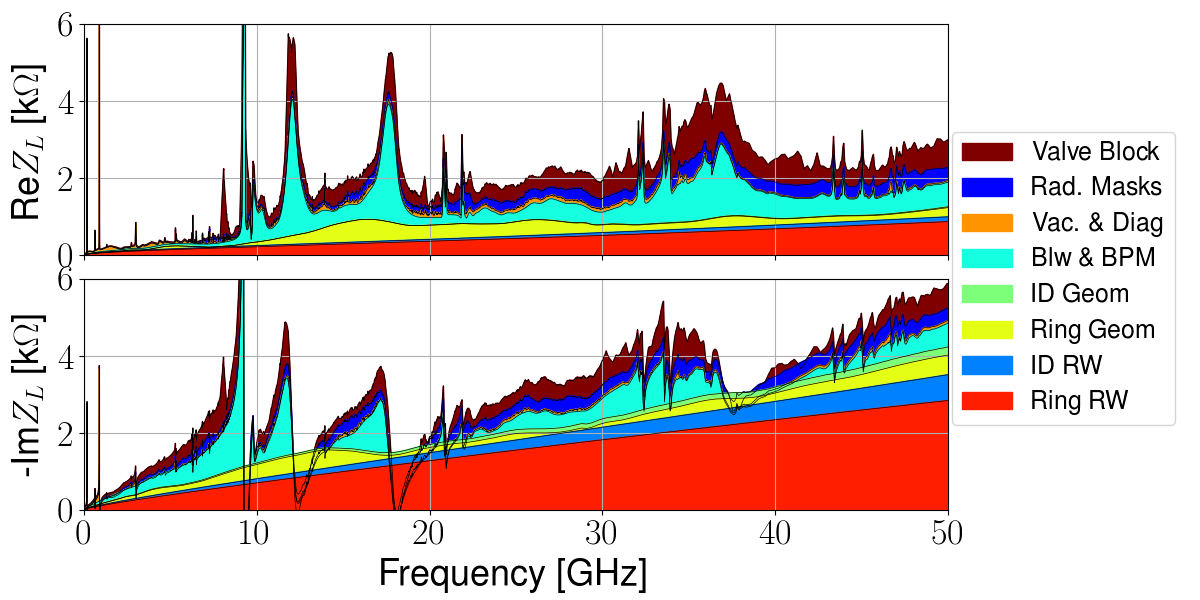
\includegraphics[width=\textwidth]{budget_ph1_imp_longitudinal.png}
        \caption{Longitudinal impedance budget for Sirius.}
        \label{fig:long_imp_budget}
    \end{figure}
    shows the longitudinal impedance budget of the storage ring for its first phase of operation and Figure~\ref{fig:ph1_kLoss_Z_eff}
    \begin{figure}
        \centering
        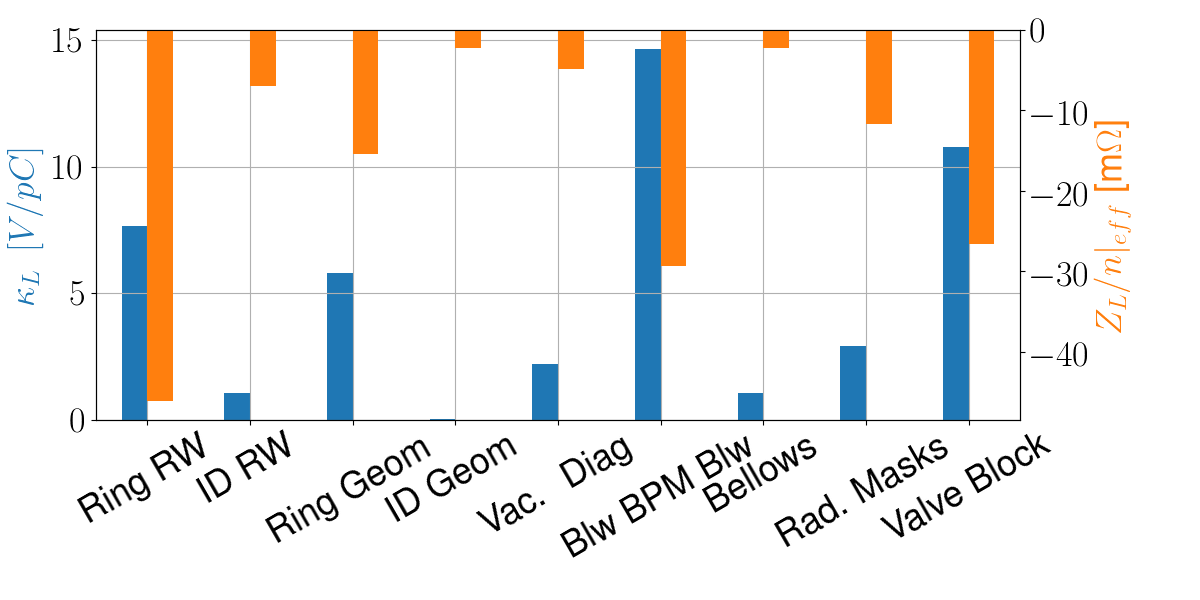
\includegraphics[width=\textwidth]{budget_ph1_kLoss_Z_eff.png}
        \caption{Single bunch Loss factor (left, blue) and effective impedance (right, orange) calculated for the nominal operation mode of phase1 for Sirius.}
        \label{fig:ph1_kLoss_Z_eff}
    \end{figure}
    shows the single bunch loss factor and effective impedance, which were defined in sections~\ref{sec:energy_loss} and~\ref{sec:mode_coupling}, respectively. Note that the imaginary part of the impedance is mostly inductive and is dominated by the resistive--wall impedance of the standard chamber, which we know from section~\ref{sec:standard_chamber} that is mostly determined by the~\gls{neg} coating. This large contribution is responsible for approximately one third of the total effective impedance of the storage ring and, consequently to the bunch lengthening, which will be discussed in Chapter~\ref{cap:instabilities_studies}.

    The second larger contribution for the imaginary part of the impedance is also the major contributor to the real part. It is common for the bellows and the \glspl{bpm} to dominate the longitudinal impedance of the ring, as can be noted from Max IV impedance budget analysed by~\citeonline{Klein2013a} or from the Soleil's, presented by~\citeonline{Nagaoka2004a} or even in the work of~\citeonline{Blednykh2007} for NSLS-II. Note in Figure~\ref{fig:long_imp_budget} the existence of three main peaks in the impedance of these components, one very narrow-band, located at approximately \SI{9}{\giga\hertz}, close but below the cutoff of the chamber,  which is due to a trapped mode in the bellows cavity. Increasing the frequency, the next one, close to \SI{12}{\giga\hertz}, also comes from the bellows, and the other, at~\SI{18}{\giga\hertz}, is from the \glspl{bpm}.
    It is interesting to note that this peak from the BPM is much broader than what was presented by~\citeonline[Figure 4a]{Duarte2013}, due to the resistive wall chamber that is included in the simulation presented here.~\citeonline{Duarte2017} shows a graphic comparing simulations with~\gls{pec} and resistive walls in GdfidL. The feature of performing electromagnetic simulations considering the finite conductivity of the metals of the chamber is reasonably new in most time domain codes, and was not available in GdfidL at the time when that paper was published.

    Considering the belows are made of stainless steel and the \glspl{bpm} are made of $\text{Ti}_\text{6}\text{Al}_\text{4}\text{V}$, the geometric average of the electrical resistivity of these materials is approximately \num{59} times larger than copper and the average length of each component is \SI{5}{\centi\meter}. Considering there will have \num{160} \glspl{bpm} and \num{360} belows in the ring, we note that this is roughly equivalent to \SI{26}{\meter} of stainless steel chamber, which in turn, because of the $\sqrt{\rho}$ dependence of the resistive wall impedance, is equivalent to ~\SI{200}{\meter} of copper chamber, qualitatively accounting for the large broad band contribution of these components. In fact, this contribution is so large that it could even change significantly value of the low frequency resistive--wall impedance and affect the thresholds for coupled--bunch instabilities in the transverse plane. It remains a task for future works to estimate this contribution and improve the impedance budget in this direction.

    The effect of the resistive--wall of the \glspl{bpm} and belows is enhanced by the fact that instead of a smooth chamber, which would distribute the impedance over the whole spectrum because of the the $1/\sqrt{\omega}$ dependence of the resistive wall, these components have cavities which increase the effective inner surface and concentrate the impedance around the frequencies of the resonant modes, which are relatively low. However, this is rather inevitable for these components, and it is worth remembering that the Sirius \gls{bpm} has one of the lowest loss factors among several existent designs due to the bell shaped cavity of its buttom, as showed by~\citeonline{Duarte2013} and its first resonant peak is at a frequency as high as it can be, considering the state of the art for the production of such component.

    Another component that is worth mentioning is the radiation mask. As described by~\citeonline{Duarte2017a} two proposals were studied, one axially symmetric, which basically creates a botleneck in the chamber, and one with only a lateral obtrusion in the inner horizontal side of the chamber, where all the radiation is concentrated. While the first design was easier and cheaper to produce, the second had a longitudinal impedance five times smaller and for this reason was chosen as the official model. Looking at Figure~\ref{fig:ph1_kLoss_Z_eff} we note that if the impedance of this component were five times larger its contribution to the budget would be as large as the one from the BPM for the loss factor, and its effective impedance would be \SI{-58}{\milli\ohm}, which is much larger than the \SI{-46}{\milli\ohm} of the resistive wall. Such significant increase would strongly impact the threshold of the microwave instability, which will be studied in Chapter~\ref{cap:instabilities_studies}.

    Figure~\ref{fig:dipolar_hor_imp_budget}
    \begin{figure}
        \centering
        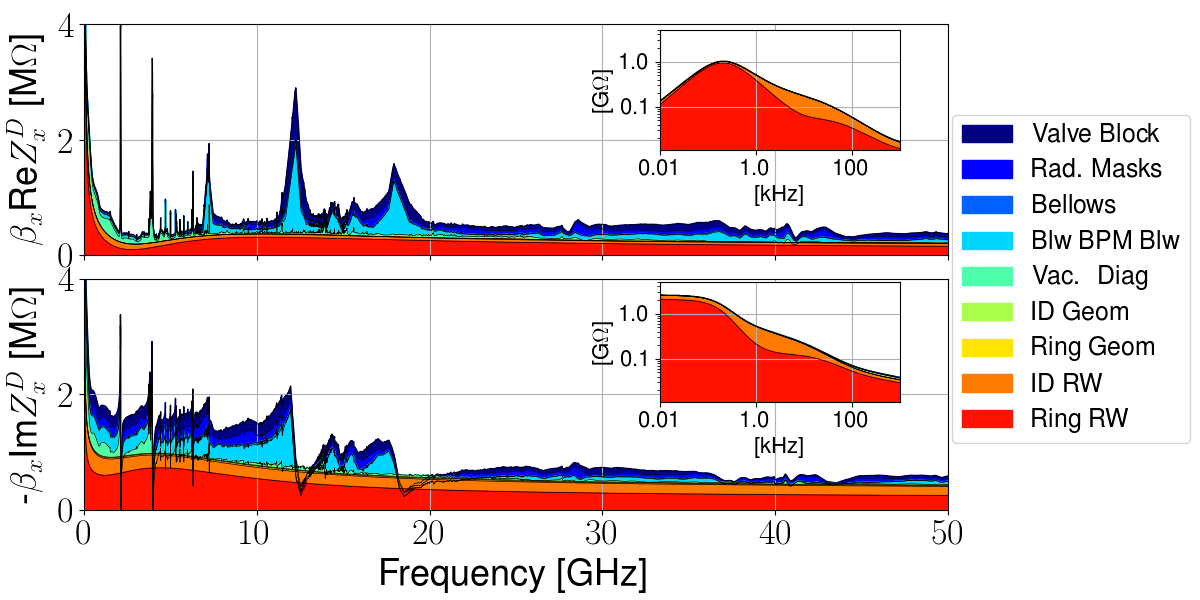
\includegraphics[width=\textwidth]{budget_ph1_imp_dip_hor.png}
        \caption{Horizontal dipolar impedance budget for Sirius.}
        \label{fig:dipolar_hor_imp_budget}
    \end{figure}
    and Figure~\ref{fig:dipolar_vert_imp_budget}
    \begin{figure}
        \centering
        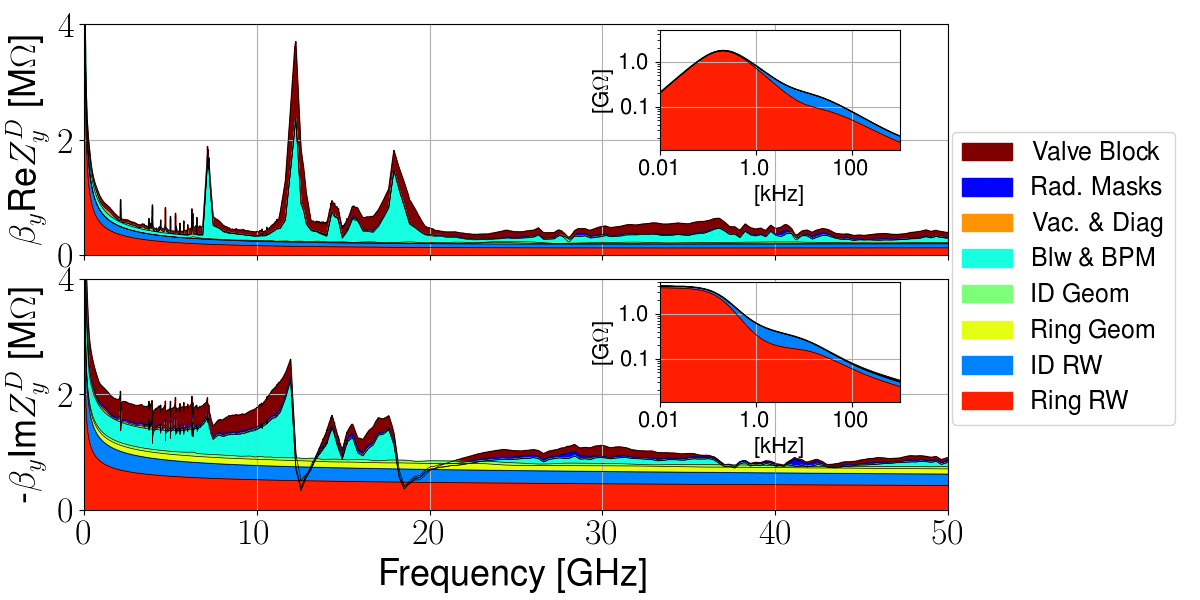
\includegraphics[width=\textwidth]{budget_ph1_imp_dip_vert.png}
        \caption{Vertical dipolar impedance budget for Sirius.}
        \label{fig:dipolar_vert_imp_budget}
    \end{figure}
    shows the $\beta_{x,y}$ weighted horizontal and vertical dipolar impedance budgets for the first phase of operation of Sirius, and Figure~\ref{fig:ph1_kickx}
    \begin{figure}
        \centering
        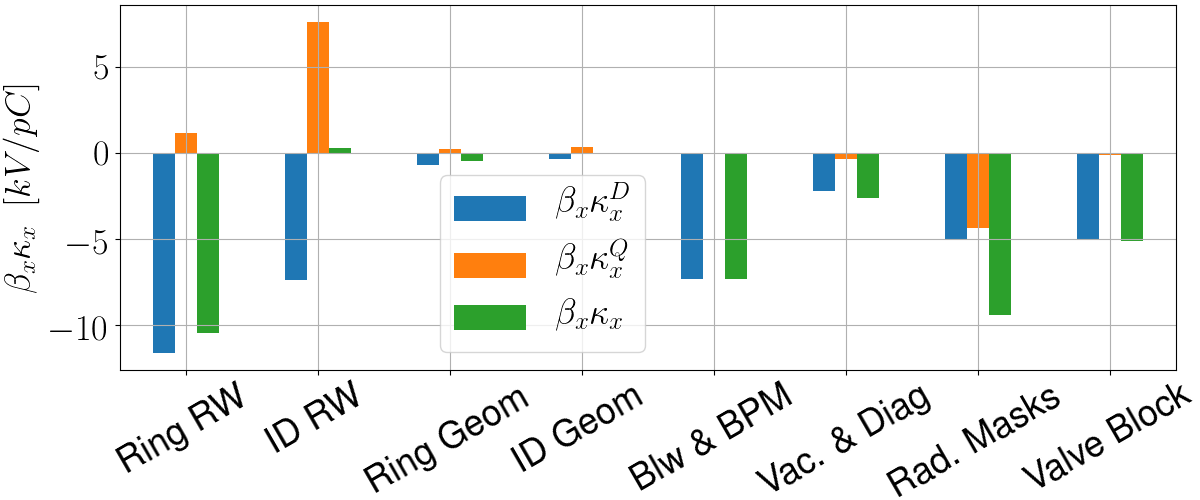
\includegraphics[width=\textwidth]{budget_ph1_kickx.png}
        \caption{Horizontal kick factors for single--bunch operation mode.}
        \label{fig:ph1_kickx}
    \end{figure}
    and Figure~\ref{fig:ph1_kicky}
    \begin{figure}
        \centering
        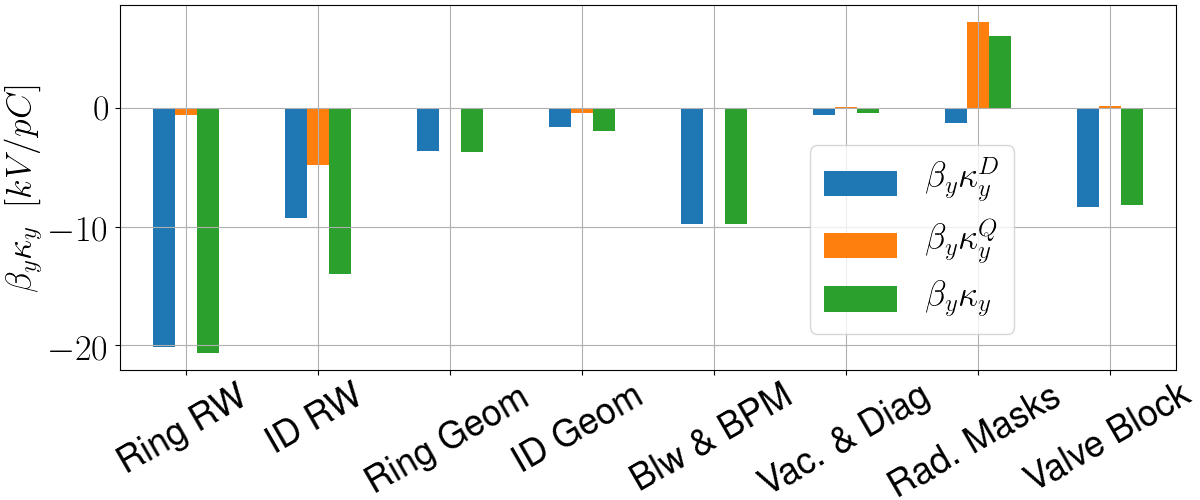
\includegraphics[width=\textwidth]{budget_ph1_kicky.png}
        \caption{Vertical kick factors for single--bunch operation mode.}
        \label{fig:ph1_kicky}
    \end{figure}
    shows the $\beta_{x,y}$ weighted single--bunch kick factor for the horizontal and vertical dipolar and quadrupolar impedances. The impedance in both planes are very similar to each other, due to the predominating round chamber of the machine. With exception of the \glspl{id}, the main differences come from the local betatron functions at the position of the components, being the vertical slightly larger, because on average $\beta_y > \beta_x$. In fact, the average of the vertical betatron function around the ring is \SI{11}{\meter}, while the horizontal is only \SI{6}{\meter}. Even though the gaps of the \glspl{id} are  very narrow and the resistive--wall impedance depends on the inverse of the cube of the half gap, the dominating contribution for the kick factors comes from the standard chambers of the ring, but only because both betatron functions at the position of the \glspl{id} are very small, of the order of \SI{3}{\meter}, as can be noticed in Table~\ref{tab:impedance_budget}.

    The only components of ring with quadrupolar impedances with significative effect on the beam for the single--bunch operation mode are the \glspl{id} and the radiation masks, due to the assymetries of their chambers. Here we recall that the quadrupolar kick factor is what originates the incoherent tune shifts of the beam and the single--bunch dipolar kick factor is related to the coherent tune  shifts, which means that their sum is the measurable tune of the machine and that last one is the main factor that determines the threshold of the \gls{tmci} instability. Considering the the vertical dipolar kick factor of the component Ring Geom is dominated by the impedance of the transition of the BC magnet, if the elliptical vacuum chamber were used instead of the keyhole geometry, as discussed in section~\ref{sec:bc_chamber}, their kick factor would be \num{2.5} times larger, being the third largest of all the groups presented here. The geometric transitions of the \glspl{id} also have a small effect on the impedance because of the low betatron function, as already explained, and due to the large transition factor, $t$, that was used in the tapers, which was only possible because the \glspl{id} are out--of--vacuum.

    While the single--bunch tune shifts are mostly defined by the broad--band impedance of the whole spectrum, their multi--bunch counterpart depends majorly on the low--frequency components of the dipolar impedance and on the zero--frequency component of the quadrupolar impedance, because, as shown in Figure~\ref{fig:dipolar_hor_imp_budget} and Figure~\ref{fig:dipolar_vert_imp_budget}, the impedance in this region is two or three orders of magnitude larger than the high--frequency part of the spectrum, being dominated by the resistive--wall contributions from the standard chamber and the undulators.
    Figure~\ref{fig:ph1_tush_multi_per_curr}
    \begin{figure}
        \centering
        \includegraphics[width=0.9\textwidth]{budget_ph1_tush_multi_per_curr.png}
        \caption{Tune shift divided by the bunch current as function of the number of bunches in uniform filling.}
        \label{fig:ph1_tush_multi_per_curr}
    \end{figure}
    shows the tune shift divided by the bunch current in uniform filling as function of the number of filled bunches, which should be an horizontal line if the impedance were broad band. When all the bunches are filled, the incoherent tune shifts are almost five times larger than the coherent ones and, in the vertical plane, most part comes from the \citeonline{Laslett1963} incoherent tune shifts from the dipole magnets, as modeled in section~\ref{sec:standard_chamber}.
    % Figure~\ref{fig:ph1_tush_wall_undu_multi_per_curr}
    % \begin{figure}
    %     \centering
    %     \includegraphics[width=0.9\textwidth]{budget_ph1_tush_wall_undu_multi_per_curr.png}
    %     \caption{Tune shift divided by the bunch current as function of the number of bunches in uniform filling.}
    %     \label{fig:ph1_tush_wall_undu_multi_per_curr}
    % \end{figure}


\chapter{Instability Studies}\label{cap:instabilities_studies}

    The impedance budget presented in the last chapter will be used here to calculate some beam parameters at equilibrium, or stationary state, and the thresholds for instabilities as well as the behavior of the beam above the threshold. It is important to remark that this is an ongoing work and the results presented here are not final. For example, the inclusion of the \gls{csr} in the budget only happened in the last month of production of this thesis (January 2018) and its tracking simulations are still being analysed for convergence. However, its large influence on the longitudinal dynamics justifies the presentation of such results.

    In the first section of this chapter we will briefly discuss the effect of the PETRA 7--Cell cavity on the coupled bunch instabilities of Sirius during commissioning; In the second section the longitudinal dynamics of the storage ring will be analysed and use the main results to study the transverse plane, in the subsequent section.

\section{The PETRA 7--Cell Cavity}

    According to the impedance budget gathered for Sirius, there will be no long--range wake fields capable of generating longitudinal coupled--bunch instabilities. All the elements simulated were tested individually to check if their impedances could to create this type of instability and none of them can do it. Actually, this was a criteria adopted in the design of the components, not only for the longitudinal plane, but also for both transverse planes. However, a PETRA 7--Cell cavity will be used in the commissioning phase and it is known that this type of cavity can generate coupled--bunch instabilities, as shown by~\citeonline{Bassi2016b} for the case of NSLS--II, for which this same commissioning strategy was adopted.~\citeonline{Bassi2016b} presents a table with the simulated values of the longitudinal \glspl{hom} of this cavity, which we will use here to estimate the instabilities for Sirius.

    The procedure we adopted to perform this analysis was the following: first we identified which of these modes have potential to cause coupled--bunch instabilities in the Sirius storage ring. This was done by finding the minimum value for the impedance as function of the frequency for which equation~\eqref{eq:long_coupled_bunch_instability} gives a positive growth rate. Isolating the impedance in that equation we get
    \begin{align}\label{eq:long_cbi_minimum_impedance}
        \left|Z_\parallel^\text{min}\fof{\omega}\right| = \frac{\omega\alpha_z}{I_T\omega_0\alpha}\frac{2\pi E_0\fof{\omega_s\sigma_z/c}^2}{h_m^2(\omega)}.
    \end{align}
    % Notice that this procedure is pessimistic, because it neglects the negavite contributions of the sampling of the negative frequencies on equation~\eqref{eq:long_coupled_bunch_instability}, which would require the difference
    % \begin{align}
    %     \real{Z\fof{\omega_0(p\pm\nu_z)} - Z\fof{\omega_0(-p\pm\nu_z)}} =
    %     \real{Z\fof{\omega_0(p\pm\nu_z)}} - \real{Z\fof{\omega_0(p\mp\nu_z)}}
    % \end{align}
    % to be larger than the \gls{rhs} of equation~\eqref{eq:long_cbi_minimum_impedance}, and not the value of the impedance.
    Figure~\ref{fig:long_cbi_minimum_impedance}
    \begin{figure}
        \centering
        \includegraphics[width=\textwidth]{long_cbi_minimum_impedance.png}
        \caption{Figure ashoelke}
        \label{fig:long_cbi_minimum_impedance}
    \end{figure}
    shows the comparison of the minimum impedance with the impedance of the cavity for different values of current, considering the azimuthal modes $m=\pm1$. For higher order azimuthal modes, the minimum impedance is much larger than any of the shunt impedances of the cavity. Note that with~\SI{10}{\milli\ampere} three modes are already larger than the minimum impedance and have potential to create instabilities.

    Next, for the modes with shunt impedance larger than the mininum impedance, we found the frequency range, $\Delta\omega_\parallel$, in which their impedance is also larger than the minimum impedance, in such a way that, recalling equation~\eqref{eq:long_coupled_bunch_instability}, if the condition
    \begin{align}
        \left.\forall p \in \mathbb{Z},\quad \exists \omega_p \in \Delta \omega \,\, \middle| \,\, \omega_p \coloneqq \omega_0\fof{Mp + \mu \pm \nu_z}\right.
    \end{align}
    is satisfied, it is very likely that the beam will be unstable. Considering the modes can be represented by the resonator impedance introduced in equation~\eqref{eq:long_resonator_impedance}, we can find $\Delta\omega_\parallel$ solving the inequality
    \begin{align}
        \left|Z_\parallel^\text{min}\right| \le \real{\frac{R_s}{1 + iQ\fof{\frac{\omega_R}{\omega}-\frac{\omega}{\omega_R}}}}
    \end{align}
    for positive frequencies. The result can be used to define
    \begin{align}
        \Delta\omega_\parallel = \left\{\omega \in \mathbb{R} \middle| -\frac{f}{2} \le \frac{\omega}{\omega_R} - \sqrt{\fof{\frac{f}{2}}^2+1} \le
        \frac{f}{2} \right\}
    \end{align}
    where $f = 1/Q\sqrt{R_s/Z_\parallel^\text{min}-1}$. In order improve the visualization of the data, it is useful to map the interval $\Delta\omega_\parallel$ for all the resonators to the interval $[0,1)$. This is accomplished with the definition
    \begin{align}\label{eq:cbi_frac_frequencies}
        \Delta\nu_\parallel = \left\{\nu \in \mathbb{R},\,\,\omega \in \Delta\omega_\parallel\,\, \middle|\,\,
        \nu=\frac{\omega}{\omega_0} - \left\lfloor\frac{\omega}{\omega_0}\right\rfloor \right\},
    \end{align}
    where $\lfloor\cdot\rfloor$ is the floor operation. In this space, the sampling lines for longitudinal instability are equal $\nu_z$ for the azimuthal mode $m=1$ and $1 - \nu_z$ for the mode $m=-1$, which are all very close to the extrems of the interval, remembering the synchrotron tune for Sirius is appximately \SI{4e-3}{}.
    Figure~\ref{fig:long_cbi_frac_frequencies}
    \begin{figure}
        \centering
        \includegraphics[width=\textwidth]{long_cbi_frac_frequencies.png}
        \caption{Figure ashoelke}
        \label{fig:long_cbi_frac_frequencies}
    \end{figure}
    shows the values of $\Delta\nu_\parallel$ as function of the coupled--bunch mode closest to each resonator,
    \begin{align}
        \mu_R \equiv \left\lfloor\frac{\omega_R}{\omega_0}\right\rfloor \text{mod}(M),
    \end{align}
    where this is strictly valid only for mode $m=1$. For mode $m=-1$ the value of $-\omega_R$ should be used, which, due to the fact that floor of negative numbers is the complement of its positive counterpart, for example, $\lfloor -3/5 \rfloor=2$, the coupled--bunch numbers would be interverted. We highlight that this definition is only useful if the bandwidth of the mode is smaller than the revolution frequency, otherwise the \gls{hom} would be able to drive more than one coupled--bunch mode. Each vertical line indicates the frequency range where instability could be generated if the beam sampled any frequency there and the horizontal black lines are the frequencies sampled by the beam.
    Analysing the Figure~\ref{fig:long_cbi_frac_frequencies} we note that according to this impedance model, the beam will be stable up to \SI{100}{\milli\ampere}. This hypotesis was tested with a direct application of the equation~\eqref{ed:long_coupled_bunch_instability}, which confirmed that there would be no positive growth rates.

    However, in the real cavity, the resonant frequencies of the~\glspl{hom} have a strong dependence on the geometry of the cavity, which, in turn, will be adjusted to change the frequency of the main mode to be close to the Sirius RF frequency and also depends on the temperature. These frequency changes can be larger than the revolution frequency of the ring, which means the scenario presented in Figure~\ref{fig:long_cbi_frac_frequencies} could change drastically and some of the modes could cross the lines sampled by the beam, close to zero and one. The first analysis, based on the results presented in Figure~\ref{fig:long_cbi_minimum_impedance}, is more reliable, because the shunt impedance is much less sensitive to small changes in the cavity. For this reason, since we plan to commission the ring with currents up to \SI{30}{\milli\ampere}, and also predicting a possible delay in the installation of the superconducting RF cavity, a longitudinal kicker was designed and will be installed in the ring, together with a longitudinal bunch--by--bunch feedback system to control the longitudinal coupled--bunch instabilities.

    This kicker will have a shunt impedance, $R_K$, of \SI{900}{\ohm} and an amplifier of \SI{30}{\watt}. Considering the losses in the cables, the maximum effective power applied to the beam will be \SI{9}{\watt}~\cite{Duarte2018}. According to~\citeonline{Lonza2007}, the relation between the power, $P$, and the damping time provided by the kicker, $\tau_K$, is given by
    \begin{align}
        \alpha_K = \frac{1}{\tau_K} =
        \sqrt{\frac{R_kP}{2}}\frac{\alpha}{2\pi\nu_z(E_0/e)}\frac{c}{z_\text{max}},
    \end{align}
    where $z_\text{max}$ is the maximum amplitude of the movement. The requirement for the maximum longitudinal oscillation of the beam for stable operation is \SI{10}{\percent} of the beam size, which corresponds to \SI{0.25}{\milli\meter} and, consequently, via the equation above, an additional damping rate of \SI{175}{\hertz} will be provided by the kicker, which is approximately two times larger than the natural damping rate of the storage ring. With this factor of three in the damping, operations with \SI{30}{\milli\ampere} will be possible. Actually, the estimative made above is pessimistic, because the measurement of the longitudinal oscillations will be much better than the requirement presented above, which means the instability will be controlled at smaller amplitudes, requiring less power. Besides, if more power were needed it will be possible to install another amplifier in parallel, doubling the total power of the system. Finally, even though Figure~\ref{fig:long_cbi_frac_frequencies} is not reliable to quantitatively describe the stability of the beam, it shows that there are regions of the $\Delta \nu$ space which are free of \glspl{hom} or at least have weaker ones, in such a way that in principle it will be possible to find more stable regions adjusting the temperature of the cavity.

    A similar study was performed for the transverse couple--bunch instabilities with the impedance model provided by~\citeonline{Bassi2016b}. In this case, we can use equation~\eqref{eq:trans_coupled_bunch_instability} to isolate the minimum impedance,
    \begin{align}
        Z_u^\text{min}(\omega) = \frac{\fof{\alpha_u + |m|\alpha_z}}{\beta_u}\frac{4\pi\nu_zE_0}{I_Th_m^2(\omega-\omega_\xi)},
    \end{align}
    where $u$ stands for both, $x$ and $y$. Figure~\ref{fig:trans_cbi_minimum_impedance}
    \begin{figure}
        \centering
        \includegraphics[width=\textwidth]{trans_cbi_minimum_impedance.png}
        \caption{Figure ashoelke}
        \label{fig:trans_cbi_minimum_impedance}
    \end{figure}
    shows the comparison of the minimum impedance with the cavity impedance for several values of currents in the machine for the azimuthal mode $m=0$. The azimuthal modes $m=\pm1$ will be stable at zero chromaticity, but at $\xi_u = 2.5$, currents larger than \SI{50}{\milli\ampere} could become unstable. The calculations were performed for the horizontal plane, but the results are identical in the vertical plane, because the horizontal and vertical betatron functions at the location of the cavity are equal to each other. In this case, there are fewer modes, but all of them are strong enough to create coupled--bunch instabilities. Even for a current as low as~\SI{5}{\milli\ampere} there are modes which could drive the beam unstable. It was verified that the chromaticity only start to influence for values larger than 5, which would degrade the lifetime of the ring and cause instabilities of the modes $m=\pm1$, as discussed above.

    Proceeding with the calculation of the frequency range, $\Delta\omega_u$ where the absolute value of the impedance for each \gls{hom} is larger than the mininum impedance, we use the equation~\eqref{eq:trans_resonator_impedance} to model the modes as resonators and get
    \begin{align}
        -Z_u^\text{min} \ge \real{\frac{\omega_R}{\omega}\frac{R_s}{1 + iQ\fof{\frac{\omega_R}{\omega}-\frac{\omega}{\omega_R}}}},
    \end{align}
    which differs from its analog in the longitudinal plane, because we are interested in negative real impedances, which are responsible for generating instabilities. This equation can be used to define, implicitly,
    \begin{align}
        \Delta\omega_u = \left\{\omega \in \mathbb{R\,\,} \middle|\,\,
        \omega < 0,\,\,\, \omega^4 + \fof{\frac{1}{Q^2}-2}\omega^2\omega_R^2 + \frac{R_s}{Z_u^\text{min}Q^2}\omega\omega_R^3 + \omega_R^4 \ge 0 \right\},
    \end{align}
    where we point out that now we are looking for negative frequencies, because it is in this region that the real part of the impedance is negative too. The second inequality in the definition of the interval $\Delta\omega_u$ is too complex to be solved analytically and the values were found numerically. With this interval, we can calculate $\Delta\nu_u$ using the exact same definition as in the longitudinal plane, given by equation~\eqref{eq:cbi_frac_frequencies}, with the remark that, since now we are working with negative frequencies, the floor operation should be carried out properly. On the other hand, the definition of the coupled--bunch mode must be changed, because the transverse tunes are much larger than unit and have to be taken in account:
    \begin{align}
        \mu_R \equiv \left\lfloor\frac{-\omega_R-\nu_u}{\omega_0}\right\rfloor \text{mod}(M).
    \end{align}
    Figure~\ref{fig:trans_cbi_frac_frequencies}
    \begin{figure}
        \centering
        \includegraphics[width=\textwidth]{trans_cbi_frac_frequencies.png}
        \caption{Figure ashoelke}
        \label{fig:trans_cbi_frac_frequencies}
    \end{figure}
    shows the fractionary frequency range, $\Delta\nu_u$ as function of the coupled--bunch mode calculated for the horizontal plane for all the transverse \glspl{hom}. Recalling equation~\eqref{eq:trans_coupled_bunch_instability}, the sampling of the impedance in the transverse plane when mapped to the space of $\Delta\nu_u$ happens at $\nu_{x,y}$, shown in the figure as black horizontal lines. Note taht the threshold for the horizontal and vertical instabilities is a little below \SI{50}{\milli\ampere}.
    Actually, the precise calculation, using equation~\eqref{eq:trans_coupled_bunch_instability}, showed that the treshold is, coincidently \SI{30}{\milli\ampere} for both planes. Besides, notice that at \SI{100}{\milli\ampere} another \gls{hom}, the same driving the vertical plane instability, also starts influence the horizontal plan. One interesting feature of this figure is that it reveals an island of stability in the region (0.34, 0.44) and, since the difference between the tunes is only \SI{0.07}{}, in principle it would be possible to try to ajust the temperature of the cavity to change the position of the \glspl{hom} in such a way that this region coincides with the beam.

    However, as discussed for the longitudinal plane, this phasing study is very ideal and it very likely that the real cavity will have a different configuration. For these reason the most pragmatic approach is to rely in transverse bunch--by--bunch feedback systems to ensure the stability of the beam. These systems will be available for Sirius in the commissioning.

\section{Longitudinal Plane}\label{sec:longitudinal_plane}

    The studies of the longitudinal dynamics of the Sirius storage ring will be presented in this section. First, we will evaluate the effects of the standard impedance budget, without considering the \gls{csr} impedance, in the second part we will analyse the noise in tracking simulations induced by high--frequency components of the wake, togheter with the solutions for this problem that were adopted in this work and in the third part we will present the results of the simulations with \gls{csr}, trying to take into account the effect of the other impedance sources and \gls{ibs} as well.

\subsection{Standard Impedance Budget Effects}\label{ssec:imp_bud_effects}

    Table~\ref{tab:sirius_main_parameters} shows only the natural, or zero--current, values of the equilibrium parameters of the storage ring. When the bunch current increases, the \gls{ibs} change these parameters due to the temperature rise coming from collisions\footnote{The effect of \gls{ibs} on Sirius equilibrium parameters was not  calculated in this work. The values shown here were obtained by Natália Milas and Afonso Haruo Mukai}. The main impact of this effect for the wake field induced collective effects is the energy spread increase and the consequent bunch lengthening.  Figure~\ref{fig:ph1_eq_param}
    \begin{figure}
        \centering
        \includegraphics[width=\textwidth]{official_phase_1_eq_param.png}
        \caption{Stationary parameters of the longitudinal plane, calculated from the solution of the Haissinski equation.}
        \label{fig:ph1_eq_param}
    \end{figure}
    shows the equilibrium parameters of the storage ring as a function of current for three situations, where the last one, \gls{ibs}$+$Wake, is not self-consistent, because it was obtained by the solution of the \citeauthor{Haissinski1973} equation using the additional energy spread induced by \gls{ibs} as initial input. It means that the reduction of the \gls{ibs} effect caused by lengthening of the bunch by the wake is not considered in that curve. While this curve can be considered as a higher limit for the bunch length and energy spread, or optimistic in relation to the threshold of the instabilities which will be studied below, the curve in which only the wake function of the machine is considered can be interpreted as the other extreme. The strong inductance of the impedance budget becomes evident in Figure~\ref{fig:ph1_eq_param} when we notice the bunch is lengthened by a factor larger than \num{2} in the current range analysed, while the synchrotron position, $\langle z \rangle$, only changes by less than \SI{2}{\milli\meter}.

    The average synchrotron tune, $\langle \nu_z \rangle$, and the synchrotron tune spread, $\sigma_{\nu_z}$, shown in Figure~\ref{fig:ph1_eq_param} were calculated based on a generalization of the synchrotron tune defined in equation~\ref{eq:synchrotron_tune} for a general voltage gap, $V(z)$. Neglecting the damping rate, $\alpha_z$, in that equation, we can define a $z$--dependent synchrotron tune as
    \begin{align}
        \nu_z(z) = \frac{1}{2\pi}\sqrt{V'(z)\alpha L_0},
    \end{align}
    where $V'(z)$ is the derivative of the effective voltage (RF cavity plus wake) obtained from the Haissinski equation, normalized by the nominal energy of the storage ring, $E_0$. This way, the average synchrotron tune and the synchrotron tune spread can be calculated with
    \begin{align}
        \langle \nu_z \rangle = \infint{x}{\nu_z(x)\lambda(x)},\quad
        \sigma_{\nu_z}^2 = \infint{x}{\fof{\nu_z(x)-\langle \nu_z \rangle}^2\lambda(x)},
    \end{align}
    respectively, where $\lambda(z)$ is the equilibrium distribution, solution of the Haissinski equation.

    The current threshold for the microwave instability was calculated in frequency domain, using equation~\eqref{eq:long_mode_coupling_instability} and by macroparticle tracking. In this process, we also created a model based on \glspl{bbr} for the whole impedance budget as an attempt to summarize it in a small set of numbers that can be used in future calculations and try to understand the individual contribution of each structure to the behavior of the beam. Such task was accomplished with the \num{11} \glspl{bbr} shown in Table~\ref{tab:resonator_model}.
    \begin{table}
        \centering
        \caption{Broad band resonators model of the Sirius longitudinal impedance budget.}
        \label{tab:resonator_model}
        \begin{tabular}{l *{10}{c}}
            \toprule
            $f_R$~[GHz]       & 716.2 & 206.9  & 138.4  &  79.6  &  57.3
            &  35.0 &  17.5  & 17.8   &  11.9  &   9.2 \\
            $R_s$~[k$\Omega$] & 30.0  &  6.5   &  2.0   &  2.0   &  2.5
            &  2.5  &  1.7   &  3.0   &  4.0   &  20.0 \\
            $Q$               &  0.7  &  1.3   &  4.0   &  1.0   &   4.5
            &  3.0  &  1.0   & 24.0   &  24.0  &  100.0 \\
            \bottomrule
        \end{tabular}
    \end{table}
    Figure~\ref{fig:ph1_imp_model_comp}
    \begin{figure}
        \centering
        \includegraphics[width=0.85\textwidth]{official_phase_1_imp_model.png}
        \caption{Comparison of the complete longitudinal impedance calculated for the Sirius storage ring (blue) with the \glspl{bbr} fitting presented in Table~\ref{tab:resonator_model} (red).}
        \label{fig:ph1_imp_model_comp}
    \end{figure}
    shows the comparison of the fitted and original impedances. Even though the agreement is not excellent and there is still room for improvement, this model explains very well the bunch lengthening, the energy loss, threshold of the instability and the behavior of the beam above the threshold. The very high frequency \gls{bbr}, the first in the table, is due to the NEG coated vacuum chamber, which has a very large inductive impedance at low frequencies, being the major contributor for the bunch lengthening and the last three resonators are originated by the bellows and the \glspl{bpm} of the machine and have a fairly large $Q$ factor. Their correct modeling was very important to reproduce the behavior of the beam above the threshold of the microwave instability.

    For the frequency domain calculations we did not take into account the \gls{ibs} effect and, due to the limitation of the theory, the potential--well distortion is not included too. We ran the simulations of the mode--coupling instability considering the first \num{31} radial modes and the azimuthal modes from \num{-30} to \num{30}, totalizing \num{1860} modes, for two different bunch lengths: \SI{2.5}{\milli\meter} and \SI{3.0}{\milli\meter}, being the first condition related to zero--current parameters of the first phase of operation of the storage ring and the second was considered only for a better understanding of the physical phenomena, as described below.
    Figure~\ref{fig:ph1_long_mode_coup}
    \begin{figure}
        \centering
        \includegraphics[width=\textwidth]{official_phase_1_long_mode_coup.png}
        \caption{Mode--coupling instability for }
        \label{fig:ph1_long_mode_coup}
    \end{figure}
    shows the results, which are amazingly interesting. There is a fierce competition for mode-coupling among modes with azimuthal number up to \num{17}, being the higher order modes driven by the strong high--frequency components of the resistive--wall impedance and the low--order modes driven by the other components of the machine, mainly the \glspl{bpm} and bellows. In the simulation with bunch length equal to \SI{2.5}{\milli\meter}, several of them couples almost togheter, being difficult to identify which one goes first. On the other hand, when a bunch of \SI{3}{\milli\meter} is used, all the coupling are shifted to higher currents and the coupling between a dipolar and a quadrupolar mode is the first one to happen. In both simulations there is the prediction of a weak instability, result of the coupling between two radial modes of the same dipolar azimuthal mode, that in fact sets the threshold for the instability at \SI{1.25}{\milli\ampere}. The \gls{bbr} model does not predict this coupling and so far we could not identify which part of the impedance budget is creating it, but it must be some component at the low--frequency part of the spectrum because it is present and unchanged in simulations with bunch lengths up to \SI{5}{\milli\meter}.

    The tracking simulations were performed for \num{3e4} turns in the ring, using \num{e7} macroparticles and the \gls{pic} method was used to apply the wake kicks, where longitudinal direction was segmented in \num{5e4} bins from \SI{-5}{\centi\meter} to \SI{5}{\centi\meter}, which corresponds to \SI{2}{\micro\meter} per bin. With these parameters all the wakes of the budget can be completely described, with the requirement of the Nyquist theorem, expressed in equation~\eqref{eq:nyquist_theorem}, being met for all of them. As will be described in the next section, the Savitzky--Golay filter was applied in the beam distribution before the convolution with wake in every turn, as an attempt to control the effects of numerical noise to acceptable levels. The initial conditions for tracking were the stationary results obtained with the Haissinski equation, to minimize the initial oscillations of the beam, which would increase the time needed for observation of the instability build up.

    Figure~\ref{fig:ph1_microwave_tracking}
    \begin{figure}
        \centering
        \includegraphics[width=\textwidth]{official_phase_1_microwave_tracking.png}
        \caption[Longitudinal beam parameters obtained from tracking.]{Main parameters of the beam obtained from tracking (dots) as function of the current for the simulations with and without the effects of \gls{ibs}. The values shown here are averages over all the \num{3e4} turns of the simulation. The solid lines are the results obtained from the solution of the Haissinski equation.}
        \label{fig:ph1_microwave_tracking}
    \end{figure}
    shows the main longitudinal beam parameters obtained from average over all the turns of the simulation. Two different situations were studied, with and without the \gls{ibs} effects, to account for the best and worst case scenarios, respectively, regarding the instability threshold. A strong instability rises between \SI{2.8}{\milli\ampere} and \SI{3.0}{\milli\ampere} for the simulation with only the wake effects, and drastically increases the average energy spread as function of the current. Only \SI{0.5}{\milli\ampere} above the threshold, the energy sread reaches values larger than the one where the effects of \gls{ibs} are considered. Even though their time average are comparable, the behavior of the beam above the threshold is completely different in both situations. This difference is evidenciated by
    Figure~\ref{fig:ph1_microwave_time_evolution}
    \begin{figure}
        \centering
        \includegraphics[width=\textwidth]{official_phase_1_microwave_time_evolution.png}
        \caption{Time evolution of the energy spread for different bunch currents close to the threshold of the saw--tooth like instability.}
        \label{fig:ph1_microwave_time_evolution}
    \end{figure}
    where the time evolution of the energy spread is shown. The coherent energy of the instability drives exponentialy increasing oscillations of the beam, deforming the longitudinal distribution of the particles. When this deformation is large, the interaction of the beam with the wake is weakened and radiation damping brings the beam to lower values of energy spread. Even though it is not shown here, simulations with a larger number of turns shows that this process of growth and damping repeats, forming a saw--tooth like pattern.
    Figure~\ref{fig:ph1_microwave_frequency}
    \begin{figure}
        \centering
        \includegraphics[width=0.8\textwidth]{official_phase_1_microwave_frequency.png}
        \caption{Discrete Fourier transform of the time dependent bunch centroid, as function of frequency in units of the zero--current synchrotron frequency.}
        \label{fig:ph1_microwave_frequency}
    \end{figure}
    shows the discrete fourier transform of the time evolution of the average bunch position, where the horizontal axis was normalized by the zero--current synchrotron tune for easy identification of the coherent modes. The dipole mode, as expected, remains fixed at one synchrotron tune, because of the single--bunch nature of the simulation, which carries the potential--well distortion togheter with the bunch.
    The mode which is driving the instability is the quadrupolar mode, close to \num{1.75}. Even though it is present in the spectrum below the threshold, its amplitude increases almost two orders of magnitude from current \SI{2.8}{\milli\ampere} to \SI{3.0}{\milli\ampere}. The peak at approximately \num{3.5} is not another coupling of modes, as Figure~\ref{fig:ph1_long_mode_coup} suggests, but only a multiple of the main mode that is driving the instability, being a result of the non-linearities created by both, the radiation damping and the different interaction of the beam with the wake as function of time.

    Figure~\ref{fig:ph1_microwave_tracking} also reveals a small sudden change in the average longitudinal position of the beam as function of the current from the simulations with \SI{2.2}{\milli\ampere} and \SI{2.4}{\milli\ampere} in both simulations presented there. This could be an indication of the weak instability predicted by the frequency domain analysis, but no other result besides this one corroborates with such interpretation, and further studies are required to confirm or reject this hypotesis.

    Even though the threshold of the instability was not determined properly with the study presented here, because the behavior of the beam in the best and worst case scenarios is completely different, two important conclusions can be taken. The first is that the lower limit for the current threshold is much larger than any current predicted for operation of the machine. Even the single--bunch operation scenarios are currently limited to \SI{2}{\milli\ampere} due to lifetime issues. The second is that, as indicated by the frequency domain analysis, the current threshold is very sentivity in relation to an increase in the bunch length caused by energy spread increase, which suggests the real behavior of the beam will be closer to the simulated \gls{ibs}$+$Wake than to the only wake case. It is a work for future endeavors, however, to develop methods to self-consistently simulate the effects of wake fields and \gls{ibs} togheter, or at least use some iterations between both isolated simulations to obtain more realistic results.

    As a final remark, the tracking code and the Haissinski solver employed in this analysis can be directly applied to determine the single--bunch stability of the storage ring in the second phase of operation, when the Landau cavity will be installed. The calculations were not performed in this work mainly due to lack of time.

\subsection{Noise in tracking simulations}\label{ssec:noise}

    Prior to the study presented above, it was necessary to deal with the problem of noise in tracking simulations in order to extract reliable results. This problem can completely spoil longitudinal simulations, because it provides an additional source of energy spread for the bunch, which is bad for two reasons: first, because this is the main observable that indicates the onset of the instability we want to study; and second, because the increased energy spread lengthens the bunch, which changes, generally weakens, the effect of the wake, preventing the instability from happening. Figure~\ref{fig:first_tracking}
    \begin{figure}
        \centering
        \includegraphics[width=\textwidth]{official_phase_1_noise_tracking.png}
        \caption{Tracking results, showing the effect of noise as a function of current for different numbers of macroparticles in the simulation.}
        \label{fig:first_tracking}
    \end{figure}
    shows an example of this phenomena, where the first tracking results obtained for Sirius are presented. They were performed with a sligthly different configuration for the machine than the one presented in last section, and for this reason this figure does not exactly compares to Figure~\ref{fig:ph1_microwave_tracking}. Note that even with a number of particles as large as \num{e6}, there still is a strong influence of noise, and only with \num{e7} particles the results seem to have converged, where the onset of an instability happens at approximately \SI{3}{\milli\ampere}, as already known from the last section results.

    This additional energy spread is introduced by the interaction of very high--frequency components of the wake with fluctuations in the beam distribution due to the finite, and reduced in relation to the real physcal system, number of particles. There are some methods to avoid this problem, being the most obvious one to increase the number of particles until this effect is negligible. This approach generally works well. For example, in the benchmarking presented in subsection~\ref{sec:tracking_code} only \num{e5} macroparticles were enough to reproduce the results of Elegant~\cite{Borland2000} and SPACE~\cite{Bassi2016}, but in the case of the impedance budget of Sirius, the strong high--frequency components of the resistive--wall and the \gls{csr}, makes such approach impracticable. Another method is to increase the size of the grids in the longitudinal plane as a method to abruptly cut the high frequencies of the wake, avoiding the generation of noise. This method is also valid when one knows that the high--frequency components of the wake are not strong enough to generate coherent motion, which again, is not the case of \gls{csr} and neither what was being indicated by the frequency--domain analysis for the case of the resistive--wall. Even when the wakes are not strong enough to create instabilities and the application of this method is viable, depending on the parameters of the simulation, convergent results might be difficult to obtain, requiring several simulations with different number of particles and mesh sizes, until optimal parameters are found.

    A conceptualy similar way of ignoring the high frequencies of the wake and, at least in parts, avoid the problem of spectral leakage is to convolve the original wake function with a small gaussian distribution, that filters out in a smoothly way the undesired frequencies without the need of increasing the mesh size and assuring the convergence of the results depends only on the number of particles. This method was successfully used for Sirius calculations considering the standard impedance budget presented in last section, but completely failed in the \gls{csr} simulations. Even the success with the impedance budget is due to the fact that, luckly, the mode which coupled first was the quadrupolar one, as showed in the last section. If the parameters of the simulation were slightly different it could have failed as well. Other filters, which are not as smooth as the gaussian could be a better alternative for handling this problem.

    Another method, which is the hard way of dealing with noise, is to filter the noise at the source, i.e. filter the distribution of particles.~\citeonline{Terzic2011} shows a very detailed study where the authors compared different methods of performing this task. The study of these advanced methods will be addressed in future works. The solution currently adopted for this problem was the use of 9--point cubic Savitzky--Golay filter~\cite{Savitzky1964}, as it is done in Elegant~\cite{Borland2000}, according to \citeonline{Borland2001}. The results presented in last section were already calculated using this method and the ones from the next section, where the \gls{csr} will be analysed will use it too.

    Considering the issues with noise are very difficult to be dealt with in tracking simulations, it is useful to know \emph{a priori} what will be its effect on the beam, given a wake function and the number of particles being simulated. This necessity motivated us to try to understand better how this coupling of the wake with the beam creates the additional energy spread. In the paragraphs below we describe a possible explanation for this process.

    Given a longitudinal density distribution $\rho(z)$, the number of particles in a small interval $\Delta z$ centered at the position $z$, $N_l(z)$, is a random variable that follows a binomial distribution. Thus, considering that there are $N_p$ macroparticles in the bunch simulation, we have
    \begin{align}
        \langle N_l \rangle = \rho(z)\Delta z N_p
        \quad \text{and}\quad
        \text{var}\fof{N_l} \approx \rho(z)\Delta z N_p,
    \end{align}
    where $\langle\cdot\rangle$ and $\text{var}\fof{\cdot}$ denotes average and variance, respectively, being the latter a measure of the fluctuations in the bunch due to the finite number of particles. If the particles were static, this fluctuation would also be, but, as they are moving due to the longitudinal dynamics of the storage ring, these fluctuations are constantly changing. For very small $\Delta z$, the value of $N_l(z)$ changes very fast, but as $\Delta z$ increases, this characteristic time becomes increasinly large.

    It is possible to estimate the length scale where the behavior of the variance changes by considering the number of turns it takes for the stored particles to complete one oscillation in the longitudinal phase space, which is $1/\nu_{z,0}$. This means that, on average, the longitudinal position of each particle differs from its position in the last turn by $\Delta z_L \approx 4\nu_{z,0}\sigma_{z,0}$. Consequently, for scales below or on the order of this length, the fluctuations of the particle distribution changes in a turn by turn basis.

    Now, let us consider there is a wake function $W(z)$ that is constant in a small interval $\Delta z_W \approx \Delta z_L$ behind the source particle and zero outside this interval. Then, any particle inside the bunch would receive random kicks $K = eI_b T_0 W N_l/N_p$. The average of this kick varies slowly in time, because it depends on the evolution of the density distribution, but the variance, given by
    \begin{align}
        \text{var}\fof{K} = \fof{qI_b T_0 W}^2 \frac{\text{var}\fof{N_l}}{N_p^2} \approx
        \fof{qI_b T_0 W}^2 \frac{\Delta z_W}{\sigma_zN_p\sqrt{2\pi \exp(1)}},
    \end{align}
    varies from turn to turn, where in the last step it was assumed $z \approx \sigma_z$ and that the distribution is gaussian, $\rho(\sigma_z)=1/(\sqrt{2\pi \exp(1)}\sigma_z)$. Summarizing, this mechanism introduce a random variation of the energy of the particles in a turn by turn basis, similarly to the quantum excitation process due to radiation emission. This means that it should change the energy spread of the beam by
    \begin{align}\label{eq:energy_spread_variation}
        \Delta \sigma^2 = \sigma_\delta^2 - \sigma_{\delta0}^2 \approx&
        \frac{4\text{var}(K)/E_0^2}{\alpha_z T_0(4-\alpha_z T_0)} =\nonumber\\
        =&\fof{\frac{qI_b T_0 W}{E_0}}^2 \frac{\Delta z_W}{\sigma_zN_p\sqrt{2\pi \exp(1)}} \frac{4}{\alpha_z T_0(4-\alpha_z T_0)}.
    \end{align}

    Figure~\ref{fig:noise_effect}
    \begin{figure}
        \centering
        \includegraphics[width=\textwidth]{official_phase_1noise_normalized.png}
        \caption[Normalized energy spread increase in Simulations induced by noise.]{Energy spread increase in simulations multiplied by $N_p\sigma_z/I_b^2$. The curves \num{e5}, \num{e6}, \num{e7} and \num{5e7} were performed with the same wake function using the \gls{pic} method, while for curve (\num{e7}, \gls{bbr}) was simulated using directly the \glspl{bbr} from the impedance model presented in subsection~\ref{ssec:imp_bud_effects}.
        For the curve (\num{e6}, Gauss) a convolution with a \SI{40}{\micro\meter} gaussian bunch was applied to the wake and a Savitzky--Golay filter was applied in the simulation of the results of (\num{e7}, Sav-Go).}
        \label{fig:noise_effect}
    \end{figure}
    shows the energy spread variation from Sirius tracking simulations multiplied by $N_p\sigma_z/I_b^2$. According to equation~\eqref{eq:energy_spread_variation} this quantity should depend only on the storage ring properties and on the wake characteristics, $(W, \Delta z_W)$, and, therefore should be an horizontal straigth line. The curves \num{e5} and \num{e6} particles approximately follow this rule, having the same baseline, and the curves \num{e7} and (\num{e7}, \gls{bbr}), deviates from this behavior above \SI{2}{\milli\ampere}, but approaches the same baseline of the others for lower currents. This deviation is understood when the simulation with \num{5e7} particles is analysed, where the real microwave instability dominates the scaling. Besides, the fact that the tracking using directly the \gls{bbr} also follows this pattern, is an indication that this is not an artefact of the \gls{pic} method.

    The curve (\num{e6}, Gauss) corresponds to the filtering of the wake with a gaussian of $\sigma=40$ \si{\micro\meter}. This filtering reduces the strength of the wake at short ranges and, consequently changes the baseline of this curve. The curve (\num{e7}, Sav-Go) is the result of using the Savitzky--Golay filter in the simulation, hence has the same short--range wake of the other curves, and, according to equation~\eqref{eq:energy_spread_variation}, should follow the same baseline of the other curves below the threshold of the instability. This is not what is happening because the filtering of the distribution changes its interaction with the high frequencies of the wake. Notice, however, that with the Savitzky--Golay filter, a simulation with \num{e7} particles have the same behavior above the threshold as a ordinary simulation with \si{5\times} more macroparticles.

    While Figure~\ref{fig:noise_effect} shows that equation~\eqref{eq:energy_spread_variation} qualitatively explains the energy spread increase induced by noise in simulations, Figure~\ref{fig:quantitative_noise_effect}
    \begin{figure}
        \centering
        \includegraphics[width=\textwidth]{official_phase_1noise_quantitative_normalized.png}
        \caption[Application of equation~\eqref{eq:energy_spread_variation} to account for energy spread increase.]{Dots represents the energy spread increase in simulations with the same wake function (represented by the blue curve in the small graphic) and lines are the prediction of equation~\eqref{eq:energy_spread_variation} using a constant model for the wake (orange line in the small graphic), with $W=1$ MV/C and $\Delta z_W = $\SI{80}{\micro\meter}.}
        \label{fig:quantitative_noise_effect}
    \end{figure}
    shows that, even though several approximations were performed in its deduction, that equation can be used to quantitatively estimate the number of particles needed to avoid such problems. In this figure the behavior of the curve (\num{e7}, Sav-Go) again differs from the others, presenting a larger energy spread increase than its counterpart without filtering for low currents, but smaller noise close to the threshold. The understanding of this behavior is a subject for further studies.

\subsection{Inclusion of \gls{csr} in the Budget}

    Before including the \gls{csr} in the Sirius impedance budget, we performed simulations using only this source of impedance to test if we could find the same threshold predicted by the theory. We ran the mode--coupling instability simulations using the first \num{30} radial numbers and  azimuthal modes from \num{-40} to \num{40}, but no instability was predicted up to \SI{4}{\milli\ampere}. Simulations with more modes were not performed because of the large time they would take. The tracking simulations were performed with the same discretization of the longitudinal direction as the one used in subsection~\ref{ssec:imp_bud_effects}, with a grid size of~\SI{2}{\micro\meter}, and the number of macroparticles was increased to \num{5e7}, to

\section{Transverse Plane}

\subsection{Multi--Bunch Instabilities}

    Differently from the longitudinal plane, in the transverse plane there will be coupled--bunch instabilities because of the long--range wake field of the resistive--wall impedance. The contribution of the \glspl{id} to this instability is two folded: on the one hand, they increase the long--range impedance of the machine, which decreases the threshold, buth on the other hand, the additional energy loss by radiation they introduce increase the damping rate in all planes, and change the equilibrium parameters of the machine, which helps stabilizing the beam. The effects of the additional radiation were calculated for the Sirius storage ring assuming all \glspl{id} were in their configuration of maximum vertical field and the main results can be found in~\cite{Sirius2013}. In practice, however, the damping rates of the machine will oscillate between the bare machine values and the maximum value presented in the mentioned reference because the \glspl{id} will be constantly moving, changing the configuration of their fields. For this reason, we decided to adopt the conservative approach and do not include the effect of the \glspl{id} on the damping time to calculate the instability thresholds.

    Figure~\ref{fig:ph1_coup_bunch}
    \begin{figure}
        \centering
        \includegraphics[width=\textwidth]{official_phase_1_coup_bunch}
        \caption{Transverse coupled--bunch instabilities for the first phase of operation of the Sirius storage ring.}
        \label{fig:ph1_coup_bunch}
    \end{figure}
    shows the coupled--bunch growth rates at zero chromaticities calculated with equation~\ref{eq:trans_coupled_bunch_instability} for the phase one of operation of the machine, with the impedance of the \glspl{id} included, but without the additional damping they provide. Besides the resistive wall instabilities, which are characterized by the peaks in the coupled--bunch numbers at $864-50=814$ in the horizontal plane and $864-15=849$ in the vertical plane, the effects of other impedances can be seen as well. In the horizontal plane the resistive wall contribution from the kickers is responsible for the slow decay of the growth rate as function of the coupled--bunch mode close the most unstable mode. This is due to the large betatron function at the injection straight section, of approximately \SI{18}{\meter}. In the vertical plane only the resistive wall is driving the beam unstable, but there is a peak at a coupled--bunch number approximately equal to 650, which is being caused by the DCCT. This component is installed in the arc of the lattice, close to the dipole B2, where the vertical betatron function is very large, of the order of \SI{22}{\meter}.

    Table~\ref{tab:ph1_coup_bunch}
    \begin{table}
        \centering
        \caption{Transverse coupled--bunch instability thresholds at zero chromaticity for the phase one of operation for different assumptions on the \glspl{id} effects.}
        \label{tab:ph1_coup_bunch}
        \begin{tabular}{lccc}
            \toprule
            \mr{3}{*}{Plane} &  \mc{3}{c}{Threshold Current [mA]} \\
            \cmidrule{2-4}
                             & \mr{2}{*}{without \glspl{id}} & \mc{2}{c}{with \glspl{id}}\\
            \cmidrule{3-4}
                             &                               & w/o damping  & with damping \\
            \midrule
            Vertical         &       29.5                    &   21.4   &   32.0  \\
            Horizontal       &       54.6                    &   37.9   &   56.8  \\
            \bottomrule
        \end{tabular}
    \end{table}
    shows the current thresholds at zero chromaticity for the coupled--bunch instabilities for different assumptions on the effect of the \glspl{id} to show their influence on the impedance budget and also the contribution of the additional damping on the stabilization of the beam. The additional damping increases the threshold by a factor of approximately~$\sfrac32$ in both planes, and, interestingly, almost cancel the effect of the impedance of the \glspl{id} for this instability. This is only possible because the betatron functions at the location of the \glspl{id} is very low, which makes their effects on the transverse dynamics to be relatively weak, even though their gap is approximately five times smaller than the standard vacuum chamber and the resistive wall goes with $1/b^3$. Table~\ref{tab:ph1_coup_bunch} also shows that the vertical threshold is almost twice as large as the one for the horizontal plane, even for the bare machine impedance, which is a consequence of the larger average vertical betatron function of the machine and the fact that the vertical tune is larger than the horizontal.

    Figure~\ref{fig:ph1_chrom_coup}
    \begin{figure}
        \centering
        \includegraphics[width=\textwidth]{official_phase_1_chrom_coup}
        \caption{Effect of chromaticity on the most unstable mode of the transverse coupled--bunch instabilities for the first phase of operation of the Sirius storage ring.}
        \label{fig:ph1_chrom_coup}
    \end{figure}
    shows the effect of the chromaticity on the most unstable mode of the coupled--bunch instability calculated with two different approaches. One using the approximate expression of equation~\ref{eq:trans_coupled_bunch_instability} for the azimuthal modes \num{0} and \num{1}, which are the diagonal terms of the mode--coupling matrix, given by equation~\ref{eq:trans_mode_coupling_instability}, and another by solving the mode--coupling matrix, considering the first \num{7} radial modes and azimuthal modes from \num{-7} to \num{7}.
    There is a very good agreement between the two approaches at low chromaticities, when the azimuthal mode \num{0} dominates the instability, but at larger values, the simplified approach overestimates the thresholds (underestimate the strength of the instability).
    This study shows that the beam will be stable when the ring is operated with chromaticities above \num{2.3} and \num{1.6} in the vertical and horizontal planes, respectively. Such dependency was foresaw a few years ago, which allowed the optimization of the non--linear optics of the storage ring to operate at chromaticity equal to \num{2.5} in both planes, which we expect will avoid the usual problems of lifetime and dynamic aperture reduction related to this type of operation.

    Even though the study above shows the possibility of operating the ring in stable conditions with an increased chromaticity, the most reliable way to solve this problem, which has been demonstrated to be successful in several \gls{3gls} along the last two decades, is the use of transverse bunch--by--bunch feedback systems. Sirius will have two of these systems, one for the horizontal plane and another for the vertical. The actuator used for them will be striplines with shunt impedance, $R_K$, of \SI{70}{\kilo\ohm\per\meter} and the amplifier will have maximum power of \SI{75}{\watt}, of which only approximately \SI{30}{\watt} will be aplicable to the beam, due to cable losses~\cite{Duarte2018}. According to~\citeonline{Lonza2007}, the relation between the power, $P$, and the damping time provided by the kicker, $\tau_K$, is given by
    \begin{align}
        \alpha_K = \frac{1}{\tau_K} =
        \sqrt{\frac{R_KP}{2}}\sqrt{\beta_K\beta_B}\frac{1}{(E_0/e)T_0}\frac{1}{x_\text{max}},
    \end{align}
    where $\beta_K$ and $\beta_B$ are the betatron functions at the position of the actuator and the pickup, respectively, and $x_\text{max}$ is the maximum amplitude of the movement. The requirement for stability of the beam allows oscillations no larger than \SI{10}{\percent} of the beam size, which corresponds to \SI{1.7}{\micro\meter} at the pickup position for the vertical plane and \SI{5.5}{\micro\meter} in the horizontal plane. These requirements for beam stability are very demanding, so we will assume, as a worst case scenario, that the instability will be controlled at an oscillation ten times larger than the requirement for the vertical plane. Using this value in the equation above, the maximum damping rate the system will be capable of controlling is \SI{170}{\kilo\hertz} and \SI{190}{\kilo\hertz} in the horizontal and vertical plane, respectively, which are much larger than the thresholds calculated so far. This estimative is, off course, very idealized, because at such large growth rates the total latency of the system, not included in this simplified analysis, becomes a serious issue, reducing the effectiveness of the bunch--by-bunch feedback system.
    Considering another scenario, where the beam is initially unstable and we want to control this instability with the feedback system, even with an oscillation as large as \SI{5}{\milli\meter}, the maximum damping rate will still be of the order of \SI{0.5}{\kilo\hertz}.

    The behavior of the beam in the second phase of operation of the storage in the multi--bunch configuration cannot be explained with the frequency domain theory used in this work because of the flattened distribution of the beam, created by the action of the passive Landau cavity, and need further investigations. However, based on the work of~\citeonline{Cullinan2016} it is expected that the chromaticity will have an even larger effect on the beam, being more efficient to stabilize it.

\subsection{Single--Bunch Instabilities}

    Figure~\ref{fig:ph1_chrom_tmci}
    \begin{figure}
        \centering
        \includegraphics[width=\textwidth]{official_phase_1_tmci}
        \caption{Transverse single--bunch instabilities for the first phase of operation of the Sirius storage ring, considering the unperturbed longitudinal distribution, without the effects of \gls{ibs} and potential--well distortion.}
        \label{fig:ph1_chrom_tmci}
    \end{figure}
    shows the growth rate of the single--bunch instability for different values of chromaticity. The solid lines represent the results obtained from tracking and the dashed lines are from the solution of the equation~\eqref{eq:trans_mode_coupling_instability}, considering the first 10 radial modes and and azimuthal modes from \num{-10} to \num{10}, totalizing \num{231} modes. The tracking simulation was performed with \num{e5} macro particles in the bunch for \num{e4} turns, using directly the effective wake functions obtained from numerical simulations with ECHO and GdfdL and the wake functions calculated with ImpedanceWake2D~\cite{Mounet2010} for the resistive--wall impedance.
    While the growth rate is a direct result of the frequency domain calculation, being given by the largest imaginary part of all the eigenvalues, for the tracking simulations it is was needed to fit linearly the natural logarithm of the beam size as function of time and take the angular coefficient in order to extract these values. The good agreement between frequency and time domain simulations shown in the Figure~\ref{fig:ph1_chrom_tmci} was already expected, considering the conditions used in tracking perfectly match the assumptions made by the mode--coupling theory.

    We do not believe that the discrepancies on the prediction of the damping rates are due to the truncation of the mode--coupling matrix, because we have performed convergence tests on the number of modes included in that analysis. They might be due to the fact that the impedance budget only have the kickers' impedance, but not the wake functions yet, which makes the total impedance and wakes of the budget not completely equivalent to each other. Another possibility comes from the fact that in the time domain simulations the effective wake functions were used, and not the point charge wakes. This could soften the strength of the short--range wakes, due to the convolution with the gaussian beam used for their calculation in the numerical solvers of the \gls{maxeq}. For future works it is recommended an investigation of better ways to extract and use the information of the effective wake functions in tracking simulations, maybe by fitting the wakes or the impedances with well--known functions, like resonators, inductors and resistors, for which analytic expressions for the wakes exists, as was done by~\citeonline{Nagaoka2006} for the Soleil impedance budget.

    Figure~\ref{fig:ph1_chrom_tmci} also shows that the chromaticity have a strong effect on the single bunch instabilities, where positive values reduce the the growth rates in both planes at the cost of lowering the current threshold too. It is expected that this reduced growth rate will improve the effectiveness of the control of this instability with the bunch--by--bunch feedback system, as shown experimentaly at ALS~\cite{Byrd1997} and at Diamond~\cite{Koukovini-Platia2017}.

    It is known from the theory, for example as explained by~\citeonline{Lindberg2016}, that the longitudinal impedance has a two folded effect on the transverse single--bunch stability because of the potential--well distortion: the reduction of the average synchrotron tune tends to decrease the threshold and the creation of synchrotron--tune spread induces Landau damping, pushing it to higher currencts. The net effect of these two mechanisms at zero chromaticity depends on the particularities of the impedance budget and need detailed analysis. The simulation of this effect on Sirius was done in a simplified manner, where the distorted potential well which generates the equilibrium distribution given by the Haissinski equation is used in the longitudinal plane to simulate the effect of the longitudinal impedance without the need of applying the wake kicks. This was done because below the threshold of the microwave instability all the effects of the longitudinal impedance are described by the distorted potential at equilibrium. This approach speeds up tracking simulations, because, besides the time saved computing the longitudinal wake kicks, it is possible to simulate much less particles without the energy spread increase coming from the coupling of the high frequency components of the wake with the noise in the particle's distribution, which can spoil the whole simulation. This method could be extended to currents higher than the threshold of the microwave instability by also adjusting the energy spread of the ring to the equilibrium energy spread defined by this instability. However, this was not done in the case of Sirius, because, as seen in section~\ref{sec:longitudinal_plane}, in the cases where the microwave instability happen it induces deformations so strong in the bunch distribution that it is not likely that a transverse instability could rise. This is an hypotesis that could be easily tested in the future using the same tools developed in this work.

    Considering the assumptions above, Figure~\ref{fig:ph1_chrom_tmci_bunlen}
    \begin{figure}
        \centering
        \includegraphics[width=\textwidth]{official_phase_1_tmci_bunlen.png}
        \caption{Transverse single--bunch instabilities for the first phase of operation of the Sirius storage ring, considering effects of \gls{ibs} and potential--well distortion.}
        \label{fig:ph1_chrom_tmci_bunlen}
    \end{figure}
    shows the effect of the longitudinal impedance on the transverse stability of the beam for two different configurations, with and without considering the effects of the \gls{ibs}, and for different values of chromaticity. In the vertical plane, the potential--well distortion alone does not increase the current threshold but helps lowering the growth rates of the instability and increase its sensitivity with chromaticity. In contrast, the additional energy spread introduced by the \gls{ibs} increases the threshold but does not influences strongly the growth rates. It is interesting to notice the peculiar behavior of the simulation with \gls{ibs} and potential--well distortion at chromaticity equals to \num{1}, where the beam is unstable from \SI{1.8}{\milli\ampere} to \SI{3.2}{\milli\ampere} and then becomes stabel againg up to currents higher than \SI{4}{\milli\ampere}.
    This can be understood if one notice that in all the situations presented in both Figure~\ref{fig:ph1_chrom_tmci} and Figure~\ref{fig:ph1_chrom_tmci_bunlen} the instability in the vertical plane is dictated by two independent mode--coupling events, being the first the responsible for the current threshold at approximately~\SI{1.45}{\milli\ampere} and the other taking place at higher currents. The qualitative behavior of the first coupling is the same in both figures, first it grows in strength up to a maximum value, which depends on the condition simulated, followed by a decline and a probable decoupling at higher currents. On the other hand, the behavior of the second coupling is very different among the simulations, being completely suppressed for chromaticities larger than \num{1} with potential--well distortion and \gls{ibs}. The qualitative behavior the instability in the horizontal plane is similar to the vertical, with the potential--well distortion alone not increasing the threshold, but helping with the strength control of the growth rates, and the \gls{ibs} contributing to the increase of the stable region.
    Finally, Figure~\ref{fig:ph1_chrom_tmci_bunlen} shows that both planes are stable when the ring is operated at a chromaticity equal to \num{2.0}.


% Finaliza a parte no bookmark do PDF, para que se inicie o bookmark na raiz
\bookmarksetup{startatroot}%

\chapter*[Conclusão]{Conclusão}
\addcontentsline{toc}{chapter}{Conclusão}
\lipsum[1-5]


% --------- Elementos pós-textuais --------------&
\postextual

% Referências bibliográficas
% \bibliographystyle{unsrt}
% \bibliographystyle{numeric}
% \bibliographystyle{plain}
\bibliography{library}
% \printbibliography


% Apêndices
\begin{apendicesenv}
% Imprime uma página indicando o início dos apêndices
\partapendices

\chapter{Lorentz Force Ultra-relativistic limit}\label{app:lorentz_cancel}
    Intuitively, we tend to think the direct interaction between charged particles, such as electric repulsion, is the responsible for the collective effects observed in storage rings, however, as we will see in the subsequent analysis, this is not the main mechanism for ultra-relativistic particles.

    \begin{figure}
	    \centering
	    \begin{tikzpicture}[scale=1]
	        \def\d{1cm}
	        \draw[<->] (1,0) node[below]{$z$}
	        -- ++(-\d,0) node[below left] {$S$}
	        -- ++(0,\d) node[left] {$\rho$}; %coord sys S
	        \draw[<->] (6*\d,0) node[below]{$z'$}
	        -- ++(-\d,0) node[below left] {$S'$}
	        -- ++(0,\d) node[left] {$\rho'$}; % coord sys S'
	        \coordinate (V) at (0.5,0);
	        \coordinate (Q1) at (4cm,1.5cm);
	        \coordinate (Q2) at (0.5cm,2.5cm);
	        \draw[->] (5*\d,0.5*\d) -- ++(V) node[above] {$\boldsymbol{v}$};
	        \filldraw[fill=black] (Q1) circle[radius=0.05] node[above] {$q$}; % source particle
	        \draw[->] (Q1) -- ++(V) node[above] {$\boldsymbol{v}$}; % velocity vector
	        \filldraw[fill=black] (Q2)  circle[radius=0.05]; % test particle
	        \draw[->] (Q2) -- ++(V) node[above] {$\boldsymbol{v}$}; % velocity vector
	        \draw[dashed,|-|] ($(Q1)-(0,0.2)$)
	        let \p1 = ($(Q2) - (Q1)$)
	        in -- ++(\x1,0) node[midway,below] {$s$}; %horizontal distance
	        \draw[dashed,|-|] ($(Q2)-(0.2,0)$)
	        let \p1 = ($(Q1) - (Q2)$)
	        in -- ++(0,\y1) node[midway,left] {$\rho$}; % vertical distance
	        \draw[->] (Q1) -- ++($(Q2) - (Q1)$) node[midway,above] {$\boldsymbol{R}$}; %vector
	    \end{tikzpicture}
	    \caption{Duas partículas interagindo via campo direto.}
        \label{fig:wake1}
    \end{figure}

    To see this lets consider the interaction of a source particle $Q$ moving with velocity $\vect{v}=v{\vect{\hat{z}}}$ with a witness particle $q$ moving with the same velocity (parallel path) at a distance $s$ in the direction parallel to the movement and at a transverse distance $\rho$, as shown in Figure\,\ref{fig:wake1}. We want to determine the force that the source particle exerts on the witness particle. One way to do this is by calculating the electric field of the source particle in the co-moving frame of reference, $S'$, and Lorentz transforming it back to the laboratory's frame. After the math we obtain:

    \begin{align}\label{eq:fields_free_particle}
    	\vect{E} = \frac{q}{4\pi\epsilon_0}\frac{\vect{R}}{\gamma^2 R^{*3}}, & & \vect{B} = \frac{1}{c^2}\vect{v} \times \vect{E}
    \end{align}
    where $\vect{R}$ is the vector which connects both particles, going from the source to the witness and  $R^{*2} = s^2 + x^2/\gamma^2$, e $\gamma = 1/(1-v^2/c^2)$.

    Combining equation~\eqref{eq:fields_free_particle} with the Lorentz force, we get the longitudinal and transverse force over the witness particle:
    \begin{align}\label{eq:space_charge_force}
    	F_l &= E_z = -\frac{q}{4\pi\epsilon_0}\frac{s}{\gamma^2\left(s^2+x^2/\gamma^2\right)^{3/2}}, \\
    	F_t &= E_x - vB_y = -\frac{q}{4\pi\epsilon_0}\frac{x}{\gamma^4\left(s^2+x^2/\gamma^2\right)^{3/2}}
    \end{align}

    In accelerator physics the force $\vect{F}$ is known as space charge force. We can infer from equation~\eqref{eq:space_charge_force} that for any position $s$ and $x$, the longitudinal force is proportional to $\gamma^{-2}$ and $F_t \sim \gamma^{-4}$ if $s \gg x/\gamma$ and  $F_t \sim \gamma^{-1}$ if $s \approx 0$. This way, in the ultra-relativistic limit, $\gamma \to \infty$, the electromagnetic interaction between particles moving parallel to each other in free space is zero. It is easy to show that in this limit, if the movement of the particles is not parallel, there is an interaction force only for $s=0$, but, as their speed is the same, this situation can only happen for an infinitesimal time.

    In this work we are interested in the the interaction between particles in the ultra-relativistic limit, $v \to c$. The space charge effects discussed above are despicable in this limit and the interaction between the particles is due to the presence of the walls of the vacuum chamber. Note that taking the limit $v \to c$ in the equation~\eqref{eq:fields_free_particle} and remembering that $s = vt - z$, we can write the electromagnetic field of a ultra-relativistic charge as
    \begin{align}
    	\vect{E} =
		\frac{q}{2\pi\epsilon_0}\frac{\vect{\hat{r}}}{r}\delta(z-ct), &
		& \vect{B} =\frac{1}{c}\vect{\hat{z}}\times\vect{E},
    \end{align}
    where $\vect{r} = \vect{\hat{x}}x + \vect{\hat{y}}y$ is a bidimensional vector in cylindrical coordinates ($\vect{\hat{x}}$ and $\vect{\hat{y}}$ are unit vectors in the $x$ e $y$ directions, respectively). The equations above show that the field is pancake-like and follow the beam as it travels through the empty space. It is important to notice that this solution is steady-state, it was necessary an infinite amount of time before $t$ to build it and that's why there is no causal paradoxes in it.

    \begin{figure}
	    \centering
	    \begin{tikzpicture}
	        \draw[very thick] (0,0) -- ++(10,0) (0,4) -- ++(10,0); %vacuum chamber
	        \draw[dashed] (0,2) -- ++(10,0); %eixo de simetria
	        \coordinate (V) at (0.5,0);
	        \coordinate (Q1) at (4cm,2.2cm);
	        \coordinate (Q2) at (0.5cm,2.5cm);
	        \filldraw[fill=black] (Q1) circle[radius=0.05] node[left] {$q$}; % source particle
	        \draw[->] (Q1) -- ++(V) node[above] {$\boldsymbol{v}$}; % velocity vector
	        \draw[-{Stealth[length=10pt]}] (Q1) let \p1 = (Q1) in --(\x1,4);
	        \draw[-{Stealth[length=10pt]}] (Q1) let \p1 = (Q1) in --(\x1,0) node[midway,right] {$\boldsymbol{E}$};
	        \draw ($(Q1)+(0,1)$) circle[radius=0.2] node[right=0.2] {$\boldsymbol{B}$};
	        \filldraw ($(Q1)+(0,1)$) circle[radius=0.07];
	    \end{tikzpicture}
	    \caption{Particles interacting in a perfectly conducting cylindrical tube.}
        \label{fig:wake2}
    \end{figure}

    Lets consider now a pipe with cylindrical symmetry\footnote{do not confuse cylindrical symmetry with cylinder. By cylindrical symmetry we mean a system with translational symmetry in one direction.}, hollow and with absolute vacuum in its interior, made of a perfect electric conductor material and with arbitrary cross section. If we put the particles of the previous example inside this pipe, moving parallel to symmetry axis, they will induce image charges in the surface of the wall which cancel the electromagnetic field inside the metal.

    The image charges travel with the same velocity $\vect{v}$ of the particles (see Figure\,\ref{fig:wake2}). As they move in parallel paths with constant velocity, in the limit $v \to c$, according to the previous results, they do not interact, independently of how close they are from each other.

    From this analysis we conclude that the interaction between particles in the ultra-relativistic limit can occur only for two reasons:
    \begin{itemize}
    \item The wall is not perfectly conducting, or
    \item The pipe does not have cylindrical symmetry (which generally is due to the presence of RF cavities, flanges, bellows, beam position monitors, vacuum pumps, among other elements in the vacuum chamber of an accelerator).
    \end{itemize}


\chapter{Duas partículas interagindo no vácuo}

    \begin{figure}
	    \centering
	    \begin{tikzpicture}[scale=1]
		    \def\d{1cm}
		    \draw[<->] (1,0) node[below]{$z$}
				-- ++(-\d,0) node[below left] {$S$}
		        -- ++(0,\d) node[left] {$\rho$}; %coord sys S
		    \draw[<->] (6*\d,0) node[below]{$z'$}
				-- ++(-\d,0) node[below left] {$S'$}
		        -- ++(0,\d) node[left] {$\rho'$}; % coord sys S'
		    \coordinate (V) at (0.5,0);
		    \coordinate (Q1) at (4cm,1.5cm);
		    \coordinate (Q2) at (0.5cm,2.5cm);
		    \draw[->] (5*\d,0.5*\d) -- ++(V) node[above] {$\boldsymbol{v}$};
		    \filldraw[fill=black] (Q1) circle[radius=0.05] node[above] {$q$}; % source particle
		    \draw[->] (Q1) -- ++(V) node[above] {$\boldsymbol{v}$}; % velocity vector
		    \filldraw[fill=black] (Q2)  circle[radius=0.05]; % test particle
		    \draw[->] (Q2) -- ++(V) node[above] {$\boldsymbol{v}$}; % velocity vector
		    \draw[dashed,|-|] ($(Q1)-(0,0.2)$)
						   let \p1 = ($(Q2) - (Q1)$)
		                   in -- ++(\x1,0) node[midway,below] {$s$}; %horizontal distance
		    \draw[dashed,|-|] ($(Q2)-(0.2,0)$)
						   let \p1 = ($(Q1) - (Q2)$)
		                   in -- ++(0,\y1) node[midway,left] {$\rho$}; % vertical distance
		    \draw[->] (Q1) -- ++($(Q2) - (Q1)$) node[midway,above] {$\boldsymbol{R}$}; %vector
	    \end{tikzpicture}
	    \caption{Duas partículas interagindo via campo direto.}
    \end{figure}

    Primeiro, campos gerados por $q_1$. No referencial $S'$:
    \begin{align}
		\vect{E'} &= \frac{q}{4\pi\epsilon_0} \frac{\vect{\hat{r'}}}{r'^2} \\
		\vect{B'} &= \vect{0'}
    \end{align}
    assumindo que a partícula 1 está na origem do sistema de coordenadas $S'$.

    Lembrando que a transformação entre coordenadas esféricas para cilíndricas são:
    \begin{align}
		r' &= \sqrt{s'^2 + \rho'^2} \\
		\vect{\hat{r'}} &= \cos\theta'\vect{\hat{z'}} +
	 				   	   \sin\theta'\vect{\hat{\rho'}} =
    	-\frac{s'}{r'}\vect{\hat{z'}} + \frac{\rho'}{r'}\vect{\hat{\rho'}}
    \end{align}
    onde a coordenada $\phi$ fica inalterada.

    Assim podemos reescrever o campo elétrico em suas partes longitudinal e transversal:
    \begin{align}
		\vect{E'}_{||} &= \frac{q}{4\pi\epsilon_0} \frac{\cos\theta'\vect{\hat{z'}}}{r'^2} =
                 	-\frac{q}{4\pi\epsilon_0} \frac{s'\vect{\hat{z'}}}{(\rho'^2+s'^2)^{3/2}} \\
		\vect{E'}_{\perp} &= \frac{q}{4\pi\epsilon_0} \frac{\sin\theta'\vect{\hat{\rho'}}}{r'^2} =
                     \frac{q}{4\pi\epsilon_0} \frac{x'\vect{\hat{\rho'}}}{(\rho'^2+s'^2)^{3/2}}
    \end{align}

    Lembrando as equações de transformação de Lorentz para campos elétricos e magnéticos, para esse problema:

    \begin{align}
 		\vect{E}_{||} &= \vect{E'}_{||}\\
 		\vect{B}_{||} &= \vect{B'}_{||}\\
 		\vect{E}_\perp &= \gamma\left(\vect{E'}_\perp - \vect{v}\times\vect{B'}\right)\\
 		\vect{B}_\perp &= \gamma\left(\vect{B'}_\perp + \frac{1}{c^2}\vect{v}\times\vect{E'}\right)
    \end{align}

    Ainda, as coordenadas espaciais são transformadas da seguinte maneira:

    \begin{align}
		\vect{\hat{\rho}} &=\vect{\hat{\rho'}}, \quad \vect{\hat{z}} = \vect{\hat{z'}}\\
		\rho &= \rho', \quad z = \frac{z'}{\gamma}
    \end{align}

    Assim, podemos notar que:

    \begin{align}
		\vect{E}_{||} &= -\frac{q}{4\pi\epsilon_0} \frac{s'\vect{\hat{z'}}}{(\rho'^2+s'^2)^{3/2}} =
				 -\frac{q}{4\pi\epsilon_0} \frac{\gamma s\vect{\hat{z}}}{((\gamma s)^2+\rho^2)^{3/2}}=
                 -\frac{q}{4\pi\epsilon_0} \frac{s\vect{\hat{z}}}{\gamma^2R^{*3}} \\
		\vect{E}_\perp&= \frac{q}{4\pi\epsilon_0}\frac{\gamma \rho'\vect{\hat{\rho'}}}{(\rho'^2+s'^2)^{3/2}} =
				 \frac{q}{4\pi\epsilon_0}\frac{\gamma \rho\vect{\hat{\rho}}}{((\gamma s)^2+\rho^2)^{3/2}}=
                 \frac{q}{4\pi\epsilon_0} \frac{\rho\vect{\hat{\rho}}}{\gamma^2R^{*3}} \\
		\vect{B}_\perp&= -\frac{\gamma   vE'_\perp}{c^2}\vect{\hat{\phi'}} =
		         -\frac{vE_\perp}{c^2}\vect{\hat{\phi}}
    \end{align}
    onde $R^* = \sqrt{s^2+\left(\rho/\gamma\right)^2}$

    Agora podemos analisar a força exercida pela partícula fonte sobre a partícula teste usando a força de Lorentz
    \begin{equation}
    	\vect{F} = \left(\vect{E} + \vect{v}\times\vect{B}\right)
    \end{equation}
    onde foi assumida carga unitária para a partícula teste, e os campos calculados anteriormente.

    Assumindo que a velocidade da partícula teste é a mesma da partícula fonte (mesmo módulo e direção), as componentes longitudinal e transversal da força ficam:

    \begin{align}
		\vect{F}_{||} &= \vect{E}_{||} = -\frac{q}{4\pi\epsilon_0} \frac{s\vect{\hat{z}}}{\gamma^2R^{*3}}\\
		\vect{F}_\perp&= \left(1+\frac{\vect{v}\times\vect{v}\times}{c^2}\right)\vect{E}_\perp =
                 \left(1-\frac{v^2}{c^2}\right)\vect{E}_\perp =
                 \frac{q}{4\pi\epsilon_0} \frac{\rho\vect{\hat{z}}}{\gamma^4R^{*3}}
    \end{align}
    onde vemos que a força longitudinal tende a zero proporcionalmente a $\gamma^{-2}$ quando $v \to c$ e que a força longitudinal tende a zero com $\gamma^{-4}$, se $s>\rho/\gamma$ e com $\gamma^{-1}$ se $s<\rho/\gamma$.

    Agora, vamos assumir que a velocidade da partícula teste não é paralela à velocidade da partícula fonte
    \begin{equation}
    	\vect{v_2} = v(\cos\delta \vect{\hat{z}} + \sin\delta\vect{\hat{\rho}})
    \end{equation}

    Assim, a força sofrida por essa partícula fica

    \begin{equation}\begin{aligned}
    	\vect{F} &= \vect{E}_{||} + \vect{E}_\perp - v(\cos\delta \vect{\hat{z}} + \sin\delta\vect{\hat{\rho}}) \times \vect{\hat{\phi}}\frac{vE_\perp}{c^2} \\
		&= \left(1-\frac{v^2}{c^2}\cos\delta\right)\vect{E}_\perp + \vect{E}_{||} + \frac{v^2}{c^2}E_\perp\sin\delta\vect{\hat{z}}
    \end{aligned}\end{equation}

    Olhando essa expressão, vemos que, conforme $v \to c$, a força pode ser expressa como:

    \begin{equation}
    	\vect{F} = \left\{
    	\begin{aligned}
    		\left((1-\cos\delta)\vect{\hat{\rho}} + \sin\delta\vect{\hat{z}}\right)
    		\frac{q}{4\pi\epsilon_0} \frac{\gamma\vect{\hat{\rho}}}{\rho^2} & &|s|<\rho/\gamma\\
    		0 & &|s|>\rho/\gamma
    	\end{aligned}\right.
    \end{equation}


\chapter{Causality and catch up distance}\label{app:causality}

    If one particle moves in a straight line at light speed, the electromagnetic field scattered by the discontinuities of the chamber will not catch up with it and will not affect the charges travelling ahead of it. The field will only interact with the charges moving behind of the source particle. Such property is known as causality.

    Even though this property is not strictly true in the real world, because particles always travel at speeds lower than the light's, it is true in most practical cases, as we will see below.

    Lets try to calculate the distance $z$ where the field generated by some discontinuity in the vacuum chamber will catch up with a witness particle at a distance $s$ behind the source particle. At the time $t=0$ the source particle passes through the discontinuity and an electromagnetic wave is generated with its wave front travelling at the speed of light in all directions, forming a sphere of radius $R$, see FigureXX. At any given time after this, the following relation holds:
    \begin{align}
		ct = R \quad vt = z && \Rightarrow && R = \frac{z}{\beta} \quad \text{where} \,\, \beta = \frac{v}{c}
    \end{align}
    where $z$ is the distance travelled by the source particle. Besides that, at the specific time when the wake catchs up with the witness particle, the following relation is valid:
    \begin{align}
		R^2 = b^2 + (z-s)^2  \Rightarrow z^2(\frac{1}{\beta^2}-1) + 2sz - (b^2 + s^2) = 0  \Rightarrow \\
		z = -\gamma^2 \beta^2 s + \sqrt{s^2\gamma^4\beta^4 + \gamma^2\beta^2\left(b^2 + s^2\right)}  = \gamma^2 \beta^2 s\left(-1 + \sqrt{1 + \frac{1}{\gamma^2\beta^2}\left(1 + \frac{b^2}{s^2}\right)}\right)
    \end{align}
    where $b$ is the distance from the discontinuity to the trajectory of the particles and $\gamma = 1/\sqrt{1-\beta^2}$ is the relativistic energy. FigureXX shows a graphic of this function, normalized by the distance $b$. We notice that, for $s=0$, which means the field catching up with the source particle, $z = \gamma\beta b$. For the case of Sirius, $\gamma \approx 5870$ and $\beta \approx 1$, if $ b = 2$mm, $z \approx 12$m.

    \begin{figure}
	    \centering
	    \label{fig:catch_up}
	    \begin{tikzpicture}
	    \draw[very thick] (0,0) -- ++(10,0) (0,4) -- ++(10,0); %vacuum chamber
	    \draw[very thick] (4.8,4) to [out=-90,in=0] (5,3.8) to [out=180,in=-90] (5.2,4);
	    \draw[dashed] (0,2) -- ++(10,0); %eixo de simetria
	    \coordinate (V) at (0.5,0);
	    \coordinate (Q1) at (4cm,2.2cm);
	    \coordinate (Q2) at (0.5cm,2.5cm);
	    \filldraw[fill=black] (Q1) circle[radius=0.05] node[left] {$q$}; % source particle
	    \draw[->] (Q1) -- ++(V) node[above] {$\boldsymbol{v}$}; % velocity vector
	    \draw[-{Stealth[length=10pt]}] (Q1) let \p1 = (Q1) in --(\x1,4);
	    \draw[-{Stealth[length=10pt]}] (Q1) let \p1 = (Q1) in --(\x1,0) node[midway,right] {$\boldsymbol{E}$};
	    \draw ($(Q1)+(0,1)$) circle[radius=0.2] node[right=0.2] {$\boldsymbol{B}$};
	    \filldraw ($(Q1)+(0,1)$) circle[radius=0.07];
	    \end{tikzpicture}
	    \caption{The catch up distance.}
    \end{figure}


    \chapter{Check Panofsky-Wenzel}\label{app:check_panofky}

    As the velocity of the particle is in the longitudinal direction we have
    \begin{align}
    	\dertot{a}{t} = \derpar{a}{t} + v\derpar{a}{s}
    \end{align}
    where $a$ can be any of the components of vector potential or the scalar potential. This way, since all fields and potentials go to zero in infinity, we always have this equality for the integral of these quantities:
    \begin{align}
    	\infint{t}{\left(\derpar{a}{t} + v\derpar{a}{s}\right)|_{s=vt-z}} = 0.
    \end{align}
    Besides, since the integration in time happens with $s=vt-z$, we have
    \begin{align}
    	\derpar{}{z}\left(\infint{t}{a}\right) =
    	\infint{t}{\derpar{a}{s}\derpar{s}{z}} =
    	-\infint{t}{\derpar{a}{s}}
    \end{align}
    Also, lets remember the relations between the electromagnetic fields and the potentials:
    \begin{align}
    	E_x &= -\derpar{A_x}{t} - \derpar{\phi}{x} &
        	& B_x = \derpar{A_y}{s} - \derpar{A_s}{y}\\
    	E_y &= -\derpar{A_y}{t} - \derpar{\phi}{y} &
        	& B_y = \derpar{A_s}{x} - \derpar{A_x}{s}\\
    	E_s &= -\derpar{A_s}{t} - \derpar{\phi}{s} &
        	& B_s = \derpar{A_x}{y} - \derpar{A_y}{x}
    \end{align}
    \begin{align}
    	w_s = \derpar{W}{z}\nonumber
    	&= \frac{c}{qQ} \derpar{}{z}\left(\infint{t}{\left(vA_s-\phi\right)}\right)
    	= \frac{c}{qQ} \infint{t}{\left(-v\derpar{A_s}{s}+\derpar{\phi}{s}\right)}\\
    	&= \frac{c}{qQ} \infint{t}{\left(\derpar{A_s}{t}+\derpar{\phi}{s}\right)}
    	=-\frac{c}{qQ} \infint{t}{E_s}\\[1cm]
    	w_x = \derpar{W}{x}\nonumber
    	&=\frac{c}{qQ} \infint{t}{\left(v\derpar{A_s}{x}-\derpar{\phi}{x}\right)}\\
    	&= \frac{c}{qQ} \infint{t}{\left(vB_y+v\derpar{A_x}{s} + E_x + \derpar{A_x}{t}\right)}
    	= \frac{c}{qQ} \infint{t}{\left(E_x + vB_y\right)}\\[1cm]
    	w_y = \derpar{W}{y}\nonumber
    	&=\frac{c}{qQ} \infint{t}{\left(v\derpar{A_s}{y}-\derpar{\phi}{y}\right)}\\
    	&=\frac{c}{qQ} \infint{t}{\left(-vB_x+v\derpar{A_y}{s} + E_y + \derpar{A_y}{t}\right)}
    	= \frac{c}{qQ} \infint{t}{\left(E_y + vB_x\right)}
    \end{align}


\chapter{Symmetry analysis}\label{app:symmetry_analysis}

    First lets consider the general expansion of the Wake potential of a bunch in the transverse coordinates of the centroid of the source $(x_s,y_s)$ and the integration path $(x,y)$ up to third order:

    \begin{align}
		W(\vect{x},s) &= W_0(s) + \sum_{i=1}^4 M_i(s) x_i + \frac12\sum_{i,j=1}^4 D_{ij}(s) x_i x_j + \frac13\sum_{i,j,k=1}^4 Q_{ijk}(s) x_i x_j x_k
    \end{align}
    where we considered $\vect{x} = (x_1,x_2,x_3,x_4) = (x_s,y_s,x,y)$ and because of the commutative property of multiplication, we can set $D_{ij} = D_{ji}$ and $Q_{ijk}=Q_{kij}=Q_{jki}=Q_{ikj}=Q_{jik}=Q_{kji}$ without loss of generality. With these considerations, number of independent components of $D$ is 10 and $Q$ is 20. Besides that, the fact that $W$ is an harmonic function of the transverse coordinates of the integration path, imposes that
    \begin{align}
		D_{33} &= - D_{44} \\
		Q_{33i} &= - Q_{44i}, \quad \text{with} \quad i=1,2,3,4
    \end{align}
    which leaves only nine independent components of $D$ and sixteen of $Q$.

    Thus, the wake forces become:
    \begin{align}
		F_L(\vec{x},s) = W'(\vec{x},s) &= W_0' + \sum_{i=1}^4 M_i' x_i + \frac12\sum_{i,j=1}^4 D_{ij}' x_i x_j + \frac13\sum_{i,j,k=1}^4 Q_{ijk}' x_i x_j x_k \\
		F_x(\vec{x},s) = \derpar{W(\vect{x},s)}{x} &= M_3 + \sum_{i=1}^4 D_{3i} x_i + \sum_{i,j=1}^4 Q_{3ij} x_i x_j \\
		F_y(\vec{x},s) = \derpar{W(\vect{x},s)}{y} &= M_4 + \sum_{i=1}^4 D_{4i} x_i + \sum_{i,j=1}^4 Q_{4ij} x_i x_j
    \end{align}

    Generally we are interested in obtaining the linear terms as function of the transverse coordinates correct up to second order. It means we want to isolate the linear from the quadract terms in the simulations. Thus, lets keep only the second order terms in the wake forces above.
    \begin{align}
		F_L(\vect{x},s) &= W_0' + \vect{M'}^T \cdot \vect{x} + \frac12\vect{x}^T \cdot \tensor{D'}  \cdot \vect{x} \\
		F_x(\vect{x},s) &= M_x + \vect{D_x}^T \cdot \vect{x} +        \vect{x}^T \cdot \tensor{Q_x} \cdot \vect{x} \\
		F_y(\vect{x},s) &= M_y + \vect{D_y}^T \cdot \vect{x} +        \vect{x}^T \cdot \tensor{Q_y} \cdot \vect{x}
    \end{align}
    where
    \begin{align}
		\vect{M} &= \begin{pmatrix*}[r] M_{1}\\ M_{2}\\ M_{3}\\ M_{4}\end{pmatrix*} \\
		\tensor{D}  &= \begin{pmatrix*}[r] D_{11} & D_{12} & D_{13} & D_{14} \\
                                   D_{21} & D_{22} & D_{23} & D_{24} \\
                                   D_{31} & D_{32} & D_{33} & D_{34} \\
                                   D_{41} & D_{42} & D_{43} & D_{44}
               \end{pmatrix*} =
               \begin{pmatrix*}[r] D_{11} & D_{12} & D_{13} & D_{14} \\
                                   D_{12} & D_{22} & D_{23} & D_{24} \\
                                   D_{13} & D_{23} & D_{33} & D_{34} \\
                                   D_{14} & D_{24} & D_{34} & -D_{33}
               \end{pmatrix*}\\
		\vect{D_x} &= \tensor{D}\cdot \vect{\hat{x}} \\
		\vect{D_y} &= \tensor{D}\cdot \vect{\hat{y}} \\
		\tensor{Q_x}&= \begin{pmatrix*}[r] Q_{311} & Q_{312} & Q_{313} & Q_{314} \\
                                   Q_{321} & Q_{322} & Q_{323} & Q_{324} \\
                                   Q_{331} & Q_{332} & Q_{333} & Q_{334} \\
                                   Q_{341} & Q_{342} & Q_{343} & Q_{344}
               \end{pmatrix*} =
               \begin{pmatrix*}[r] Q_{113} & Q_{123} & Q_{133} & Q_{134} \\
                                   Q_{123} & Q_{223} & Q_{233} & Q_{234} \\
                                   Q_{133} & Q_{233} & Q_{333} & Q_{334} \\
                                   Q_{134} & Q_{234} & Q_{334} & -Q_{333}
               \end{pmatrix*}\\
		\tensor{Q_y}&= \begin{pmatrix*}[r] Q_{411} & Q_{412} & Q_{413} & Q_{414} \\
                                   Q_{421} & Q_{422} & Q_{423} & Q_{424} \\
                                   Q_{431} & Q_{432} & Q_{433} & Q_{434} \\
                                   Q_{441} & Q_{442} & Q_{443} & Q_{444}
               \end{pmatrix*} =
               \begin{pmatrix*}[r] Q_{114} & Q_{124} & Q_{134} & Q_{133} \\
                                   Q_{124} & Q_{224} & Q_{234} & Q_{233} \\
                                   Q_{134} & Q_{234} & Q_{334} & -Q_{333} \\
                                   Q_{133} & Q_{233} &-Q_{333} & -Q_{334}
               \end{pmatrix*}\\
    \end{align}



    Due to their importance, some components of the $D$ tensor have a name: the $D_{31}$ and $D_{42}$ are called dipolar wakes; and $D_{33}$ and $D_{44}$ are the quadrupolar wakes. While the first generates coherent tune--shifts and instabilities, the later is the responsible for incoherent tune--shifts of the beam. The other terms are the skew components, which are zero for most practical cases, as we will see below.

    When the geometry has symmetry the number of independent compononts in $M$, $D$ and $Q$ are reduced even more.
    When the symmetry occurs in one plane, the number of independent components is two, five and eight, respectivelly.Below we list examples for the most practical cases:

    \begin{itemize}
    \item symmetry in the $yz$ plane, or $x=0$.
    \begin{align}
		W(x_s,y_s,x,y,s) = & W(-x_s,y_s,-x,y,s) \Rightarrow \\
		M_2= & M_4=0\\
		D_{12}=D_{14}= & D_{23}=D_{34}=0\\
		Q_{111}=Q_{122}= & Q_{113}=Q_{223}=0\\
		Q_{133}=Q_{333}= & Q_{124}=Q_{234}=0
    \end{align}
    \begin{align}
		\vect{M}&= \begin{pmatrix} M_{1}\\ 0\\ M_{3}\\ 0\end{pmatrix} &
		\tensor{D} &= \begin{pmatrix} D_{11} &    0   & D_{13} &    0    \\
                                  0   & D_{22} &    0   &  D_{24} \\
                               D_{13} &    0   & D_{33} &    0    \\
                                  0   & D_{24} &    0   & -D_{33}
               \end{pmatrix}\\
		\tensor{Q_x}&=\begin{pmatrix}    0    & Q_{123} &    0    & Q_{134} \\
                               Q_{123} &    0    & Q_{233} &    0    \\
                                  0    & Q_{233} &    0    & Q_{334} \\
                               Q_{134} &    0    & Q_{334} &    0
               \end{pmatrix} &
		\tensor{Q_y}&=\begin{pmatrix} Q_{114} &    0    & Q_{134} &    0    \\
                                  0    & Q_{224} &    0    & Q_{233} \\
                               Q_{134} &    0    & Q_{334} &    0    \\
                                  0    & Q_{233} &    0    & -Q_{334}
               \end{pmatrix}
    \end{align}

    \item symmetry in the $xz$ plane, or $y=0$.
    \begin{align}
		W(x_s,y_s,x,y,s) = & W(x_s,-y_s,x,-y,s) \Rightarrow \\
		M_1= & M_3=0\\
		D_{12}=D_{14}= & D_{23}=D_{34}=0\\
		Q_{112}=Q_{222}= & Q_{123}=Q_{233}=0\\
		Q_{114}=Q_{224}= & Q_{134}=Q_{334}=0
    \end{align}
    \begin{align}
		\vect{M}    &= \begin{pmatrix}   0  \\ M_{2}\\  0  \\ M_{4}\end{pmatrix} &
		\tensor{D}  &= \begin{pmatrix} D_{11} &    0   & D_{13} &    0   \\
                                  0   & D_{22} &    0   & D_{24} \\
                               D_{13} &    0   & D_{33} &    0   \\
                                  0   & D_{24} &    0   & -D_{33}
               \end{pmatrix}\\
		\tensor{Q_x}&= \begin{pmatrix} Q_{113} &    0    & Q_{133} &    0    \\
                                  0    & Q_{223} &    0    & Q_{234} \\
                               Q_{133} &    0    & Q_{333} &    0    \\
                                  0    & Q_{234} &    0    & -Q_{333}
               \end{pmatrix} &
		\tensor{Q_y}&= \begin{pmatrix}    0    & Q_{124} &    0    & Q_{133} \\
                               Q_{124} &    0    & Q_{234} &    0    \\
                                  0    & Q_{234} &    0    & -Q_{333} \\
                               Q_{133} &    0    &-Q_{333} &    0
               \end{pmatrix}
    \end{align}

    \item symmetry in the plane $y=x$.
    \begin{align}
		W(x_s,y_s,x,y,s) =& W(y_s,x_s,y,x,s) \Rightarrow \\
		M_1=M_2, \quad & M_3=M_4\\
		D_{11}=D_{22}, \quad D_{13}=D_{24}, \quad & D_{14}=D_{23}, \quad D_{33}=0 \\
		Q_{111}=Q_{222}, \quad Q_{112}= Q_{122}, \quad & Q_{113}=Q_{224}, \quad Q_{114}= Q_{223} \\
		Q_{123}=Q_{124}, \quad Q_{133}=-Q_{233}, \quad & Q_{134}=Q_{234}, \quad Q_{333}=-Q_{334}
    \end{align}
    \begin{align}
		\vect{M}  &= \begin{pmatrix} M_{1}\\ M_{1}\\ M_{3}\\ M_{3}\end{pmatrix} &
		\tensor{D}   &=\begin{pmatrix} D_{11} & D_{12} & D_{13} & D_{14} \\
                               D_{12} & D_{11} & D_{14} & D_{13} \\
                               D_{13} & D_{14} &    0   & D_{34} \\
                               D_{14} & D_{13} & D_{34} &    0
               \end{pmatrix}\\
		\tensor{Q_x}&= \begin{pmatrix} Q_{113} & Q_{123} & Q_{133} & Q_{134} \\
                               Q_{123} & Q_{114} &-Q_{133} & Q_{134} \\
                               Q_{133} &-Q_{133} & Q_{333} &-Q_{333} \\
                               Q_{134} & Q_{134} &-Q_{333} &-Q_{333}
               \end{pmatrix} &
		\tensor{Q_y} &=\begin{pmatrix} Q_{114} & Q_{123} & Q_{134} & Q_{133} \\
                               Q_{123} & Q_{113} & Q_{134} &-Q_{133} \\
                               Q_{134} & Q_{134} &-Q_{333} &-Q_{333} \\
                               Q_{133} &-Q_{133} &-Q_{333} & Q_{333}
               \end{pmatrix}
    \end{align}

    \item symmetry in the plane $y=-x$.
    \begin{align}
		W(x_s,y_s,x,y,s) =& W(-y_s,-x_s,-y,-x,s) \Rightarrow \\
		M_1=-M_2, \quad & M_3=-M_4\\
		D_{11}=D_{22}, \quad D_{13}=D_{24}, \quad & D_{14}=D_{23}, \quad D_{33}=0 \\
		Q_{111}=-Q_{222}, \quad Q_{112}=-Q_{122}, \quad & Q_{113}=-Q_{224}, \quad Q_{114}=-Q_{223} \\
		Q_{123}=-Q_{124}, \quad Q_{133}= Q_{233}, \quad & Q_{134}=-Q_{234}, \quad Q_{333}= Q_{334}
    \end{align}
    \begin{align}
		\vect{M}  &= \begin{pmatrix} M_{1}\\ -M_{1}\\ M_{3}\\ -M_{3}\end{pmatrix} &
		\tensor{D}   &=\begin{pmatrix} D_{11} & D_{12} & D_{13} & D_{14} \\
                               D_{12} & D_{11} & D_{14} & D_{13} \\
                               D_{13} & D_{14} &    0   & D_{34} \\
                               D_{14} & D_{13} & D_{34} &    0
               \end{pmatrix}\\
		\tensor{Q_x}&= \begin{pmatrix} Q_{113} & Q_{123} & Q_{133} & Q_{134} \\
                               Q_{123} &-Q_{114} & Q_{133} &-Q_{134} \\
                               Q_{133} & Q_{133} & Q_{333} & Q_{333} \\
                               Q_{134} &-Q_{134} & Q_{333} &-Q_{333}
               \end{pmatrix} &
		\tensor{Q_y} &=\begin{pmatrix} Q_{114} &-Q_{123} & Q_{134} & Q_{133} \\
                              -Q_{123} &-Q_{113} &-Q_{134} & Q_{133} \\
                               Q_{134} &-Q_{134} & Q_{333} &-Q_{333} \\
                               Q_{133} & Q_{133} &-Q_{333} &-Q_{333}
               \end{pmatrix}
    \end{align}
    \end{itemize}

    Below we combine some of the above mentioned symmetries which are very common in the simulations performed for accelerators elements:

    \begin{itemize}
    \item x=0 and y=0.
    \begin{align}
		\vect{M}= \vect{0} & &
		\tensor{D} = \begin{pmatrix} D_{11} &    0   & D_{13} &    0    \\
                                  0   & D_{22} &    0   &  D_{24} \\
                               D_{13} &    0   & D_{33} &    0    \\
                                  0   & D_{24} &    0   & -D_{33}
               \end{pmatrix} & &
		\tensor{Q_x}=\tensor{0} & &
		\tensor{Q_y}=\tensor{0}
    \end{align}

    \item $y=-x$ and $y=x$.
    \begin{align}
		\vect{M}= \vect{0} & &
		\tensor{D}   &=\begin{pmatrix} D_{11} & D_{12} & D_{13} & D_{14} \\
                               D_{12} & D_{11} & D_{14} & D_{13} \\
                               D_{13} & D_{14} &    0   & D_{34} \\
                               D_{14} & D_{13} & D_{34} &    0
               \end{pmatrix}& &
		\tensor{Q_x}=\tensor{0} & &
		\tensor{Q_y}=\tensor{0}
    \end{align}

    \item $x=0$, $y=0$, $y=-x$ and $y=x$.
    \begin{align}
		\vect{M}= \vect{0} & &
		\tensor{D}   &=\begin{pmatrix} D_{11} &   0    & D_{13} &   0    \\
                                 0    & D_{11} &    0   & D_{13} \\
                               D_{13} &   0    &    0   &   0    \\
                                 0    & D_{13} &    0   &   0
               \end{pmatrix} & &
		\tensor{Q_x}=\tensor{0} & &
		\tensor{Q_y}=\tensor{0}
    \end{align}
    \end{itemize}
    where we notice that when there is at least 2 planes of symmetry, all the odd order terms are zero.


\chapter{Wake Calculation From GdfidL Simulations} \label{app:wake_from_gdfidl}

    One simulation in GdfidL consists of passing a linear gaussian bunch with the velocity of light in the longitudinal direction and with a specific transverse position, say $(x_s,y_s)=(d_x,d_y)$ through the simulated structure solving Maxwell equations in time. While doing this, the code saves in memory the wake potential $W(d_x,d_y,x,y,s)$ for all transverse positions $(x,y)$ of integration and all $s$. This procedure is very time consuming and we gerally try to perform the mininum amount of simulations possible to get the results we need.

    Lets suppose a simulation was performed with the position of the source in $(x_s,y_s)=(d,0)$. If we calculate the Horizontal Wake potential in a path where $y=0$ then, up to second order in the transverse coordinates we can write:

    \begin{align}
		F_L(d,0,x,0) &= W_0  +  M_1d  +  M_3x + D_{11}d^2 + D_{13}dx + D_{33}x^2 \\
		F_x(d,0,x,0) &= M_x + D_{x3} x + D_{x1} d + Q_{x33} x^2 + Q_{x11} d^2 + Q_{x13} x d\\
		F_y(d,0,x,0) &= M_y + D_{y3} x + D_{y1} d + Q_{y33} x^2 + Q_{y11} d^2 + Q_{y13} x d
    \end{align}

    Now, integrating the total wake in 4 different $x$ points we get:
    \begin{align}
		F_1 = F_x(d,x_1) &= M_x  +  D_{x3} x_1  +  D_{x1} d  +  Q_{x33} x_1^2  +  Q_{x11} d^2  +  Q_{x13} x_1 d \\
    	F_2 = F_x(d,x_2) &= M_x  +  D_{x3} x_2  +  D_{x1} d  +  Q_{x33} x_2^2  +  Q_{x11} d^2  +  Q_{x13} x_2 d \\
    	F_3 = F_x(d,x_3) &= M_x  +  D_{x3} x_3  +  D_{x1} d  +  Q_{x33} x_3^2  +  Q_{x11} d^2  +  Q_{x13} x_3 d \\
    	F_4 = F_x(d,x_4) &= M_x  +  D_{x3} x_4  +  D_{x1} d  +  Q_{x33} x_4^2  +  Q_{x11} d^2  +  Q_{x13} x_4 d
    \end{align}

    To extract the component $D_x$ from the total wake we do:
    \begin{align}
		\Delta_1 = \frac{F_1}{x_1} - \frac{F_2}{x_2} &= \left(M_x  +  D_{x1}d  +  Q_{x11}d^2\right)\left(\frac{1}{x_1}-\frac{1}{x_2}\right) + Q_{x33}(x_1-x_2) \\
		\Delta_2 = \frac{F_3}{x_3} - \frac{F_4}{x_4} &= \left(M_x  +  D_{x1}d  +  Q_{x11}d^2\right)\left(\frac{1}{x_3}-\frac{1}{x_4}\right) + Q_{x33}(x_3-x_4)
    \end{align}
    then, remembering $(1/a-1/b)/(a-b) = -1/ab$ we get:
    \begin{align}
		\frac{\Delta_1}{x_1-x_2} - \frac{\Delta_2}{x_3-x_4} &= \left(M_x  +  D_{x1} d  +  Q_{x11} d^2\right)\left(\frac{1}{x_3x_4} - \frac{1}{x_1x_2}\right)
    \end{align}
    \begin{align}
		M_x  +  D_{x1} d +  Q_{x11} d^2 &= \left(\frac{x_1x_2x_3x_4}{x_3x_4 - x_1x_2}\right)\left(\frac{\Delta_1}{x_1-x_2} - \frac{\Delta_2}{x_3-x_4}\right)
    \end{align}

    Note that in general to isolate the dipolar component $D_x$, it is necessary to perform another two simulations. If another simulation is performed with the source at $(x_s,y_s) = (-d,0)$ it is also possible to isolate the dipolar component.

    Now, lets try to extract the quadrupolar component
    \begin{align}
		\Delta_1 = \frac{F_1 - F_2}{x_1-x_2} &= D_{x3} + Q_{x13}d + Q_{x33}(x_1 + x_2)
    \end{align}
    Notice that, if we choose $x_2=-x_1$ the contribution from $Q_{x33}$ is canceled and
    \begin{align}
		D_{x3} + Q_{x13}d = \Delta_1
    \end{align}
    where it is clear that is necessary other simulation to extract the quadrupolar wake.


\chapter{ECHOzR Post--Processing} \label{app:wake_from_echozr}

    According to~\citeonline{Zagorodnov2015} the wake functions are given by
    \begin{align}
		W_{||}(x_0,y_0,x,y,s) &=
            \frac1w\sum_{m=1}^\infty W_m(y_0,y,z)\sin(k_{x,m}x_0)\sin(k_{x,m}x), \\[4mm]
		W_y(x_0,y_0,x,y,s) &=
            \frac1w\sum_{m=1}^\infty k_{x,m}W_{y,m}(y_0,y,z)\sin(k_{x,m}x_0)\sin(k_{x,m}x), \\[4mm]
		W_x(x_0,y_0,x,y,s) &=
            \frac1w\sum_{m=1}^\infty k_{x,m}W_{x,m}(y_0,y,z)\sin(k_{x,m}x_0)\cos(k_{x,m}x),
    \end{align}
    where $w$ is the half-width of the structure, $0<x<2w$ is the horizontal position of the trailing particle, $0<x_0<2w$ is the horizontal position of the source particle, $y$ is vertical position of the trailing particle, $y_0$ is vertical position of the source particle, $z=ct-s$ is the position of the trailing particle relative to the source particle and
    \begin{equation}
    k_{x,m} = \frac{\pi}{2w}m
    \end{equation}
    The other terms are given by
    \begin{align}
		W_m(y_0,y,s)     = &W^{cc}_m(s)\cosh(k_{x,m}y_0)\cosh(k_{x,m}y) +\\\nonumber
                           &W^{ss}_m(s)\sinh(k_{x,m}y_0)\sinh(k_{x,m}y), \\[4mm]
		W_{y,m}(y_0,y,s) = &S^{cc}_m(s)\cosh(k_{x,m}y_0)\sinh(k_{x,m}y) +\\\nonumber
                           &S^{ss}_m(s)\sinh(k_{x,m}y_0)\cosh(k_{x,m}y), \\[4mm]
		W_{x,m}(y_0,y,s) = &S^{cc}_m(s)\cosh(k_{x,m}y_0)\cosh(k_{x,m}y) +\\\nonumber
                           &S^{ss}_m(s)\sinh(k_{x,m}y_0)\sinh(k_{x,m}y),
    \end{align}
    where
    \begin{align}
		S^{cc}_m = \int_{-\infty}^s W^{cc}_m(s')\mathrm{d}s', \qquad S^{ss}_m = \int_{-\infty}^s W^{ss}_m(s')\mathrm{d}s'
    \end{align}
    and the quantities $W^{cc}_m(s')$ and $W^{ss}_m(s')$ are related to the output of the softwares ECHOzR and ECHO2D by:
    \begin{align}
		W^{cc}_m(s') = \frac{W_m^M(y_0,y,s)}{\cosh(k_{x,m}y_0)\cosh(k_{x,m}y)} \\[4mm]
		W^{ss}_m(s') = \frac{W_m^E(y_0,y,s)}{\sinh(k_{x,m}y_0)\sinh(k_{x,m}y)}
    \end{align}
    where $W_m^M(y_0,y,s)$ and $W_m^M(y_0,y,s)$ are the results of the simulation with magnetic and electric boundary conditions, respectively.


    Our objective is to obtain the formulas for the monopole longitudinal, dipole and quarupolar transverse wake functions at the point $\vec{v} = (x_0=w,y_0=0,x=w,y=0)$ from these results. The monopolar wakes are readly obtained:
    \begin{align}
		W_m(0,0,s) = W^{cc}_m(s) &\Rightarrow W_{||}(\vec{v}) = \frac1w\sum^\infty_{m=1,\mathrm{odd}} W^{cc}_m(s), \\[4mm]
		W_{y,m}(0,0,s) = 0 &\Rightarrow W_y(\vec{v}) = 0, \\[4mm]
		W_{x,m}(0,0,s) = S^{cc}_m(s) &\Rightarrow W_x(\vec{v}) = \frac1w\sum^\infty_{m=1} S^{cc}_m(s)\frac{\sin(m\pi)}{2} = 0
    \end{align}
    To calculate the dipolar and quadrupolar wakes, we need to take the first derivative of the transverse wakes at the point of interest, $\vec{v}$. It is easy to see that the first derivatives of the longitudinal wake are zero. For the transverse:

    \begin{align}
		W_{y,d}(s) &= \left.\frac{\mathrm{d}}{\mathrm{d}y_0}W_y\right|_{\vec{v}} = \frac1w\sum^\infty_{m=1,\mathrm{odd}} k_{x,m}^2 S^{ss}_m(s) = \frac1w\int_{-\infty}^s\sum^\infty_{m=1,\mathrm{odd}} k_{x,m}^2 W^{ss}_m(s') \mathrm{d}s',\\[4mm]
		W_{y,q}(s) &= \left.\frac{\mathrm{d}}{\mathrm{d}y}W_y\right|_{\vec{v}} = \frac1w\sum^\infty_{m=1,\mathrm{odd}} k_{x,m}^2 S^{cc}_m(s) = \frac1w\int_{-\infty}^s\sum^\infty_{m=1,\mathrm{odd}} k_{x,m}^2 W^{cc}_m(s') \mathrm{d}s', \\[4mm]
		W_{x,d}(s) &= \left.\frac{\mathrm{d}}{\mathrm{d}x_0}W_x\right|_{\vec{v}} = \frac1w\sum^\infty_{m=1,\mathrm{even}} k_{x,m}^2 S^{cc}_m(s) = \frac1w\int_{-\infty}^s\sum^\infty_{m=1,\mathrm{even}}k_{x,m}^2 W^{cc}_m(s') \mathrm{d}s', \\[4mm]
		W_{x,q}(s) &= \left.\frac{\mathrm{d}}{\mathrm{d}x}W_x\right|_{\vec{v}} = -\frac1w\sum^\infty_{m=1,\mathrm{odd}} k_{x,m}^2 S^{cc}_m(s) =-\frac1w\int_{-\infty}^s\sum^\infty_{m=1,\mathrm{odd}} k_{x,m}^2 W^{cc}_m(s') \mathrm{d}s'
    \end{align}
    and all the skew terms are zero.


\chapter{Passive Landau cavity simulation}\label{eq:passive_landau_cavity}

    Assuming the wake function of the main mode of the Landau cavity can be modeled by the longitudinal resonator impedance with parameters $\omega_R$, $R$ and $Q$:
    \begin{align}\label{eq:longitudinal_resonator_wake}
        W'_0(z) = 2\alpha Re^{-\alpha z/c}\left(\cos\left(\frac{\bar{\omega}_Rz}{c}\right)-
                                \frac{\alpha}{\bar{\omega}_R}
                                    \sin\left(\frac{\bar{\omega}_Rz}{c}\right)\right)
    \end{align}
    where $\alpha = \omega_R/2Q$, $\bar{\omega}_R=\sqrt{\omega_R^2-\alpha^2}$, then, the equilibrium normalized potential in the cavity is given by:
    \begin{align}\label{eq:total_potential}
        V_n(z) = \frac{eC_0}{cE_0}2\alpha R\left(\real{\hat{V}_n(z)}+\frac{\alpha}{\bar{\omega}_R}\imag{\hat{V}_n(z)}\right)
    \end{align}
    where $C_0$ is the ring circumference, $e$ is the electron charge, $E_0$ is the average energy of the storage ring and $c$ is the speed of light in vacuum. The subscript $n$ indicates we want to know the potential in the $n$-th bunch. The term $\hat{V}_n(z)$ is the infinite sum of the potentials deposited by each bunch in the structure in previous turns:
    \begin{align}
        \hat{V}_n(z) = \sum_{l\in\mathscr{B}} \sum_{k=a_l}^\infty I_l e^{-\beta (s_l(k) - s_n(0)-z)}=
                    e^{\beta z}\sum_{l\in\mathscr{B}}I_l e^{\beta(n-l)\frac{C_0}{h}}
                    \overbrace{\sum_{k=a_l}^\infty e^{-\beta k C_0}}^{A_l}
    \end{align}
    where $\beta = (\alpha + i \hat{\omega}_R) / c$, $I_l$ is the current of the $l$-th bunch, $h$ is the harmonic number, $s_l(k)$ indicates the synchrotron position of the $l$-th bunch $k$ turns behind the current one, $\mathscr{B}$ is the set of all the bunch numbers that are filled and
    \begin{align}
        a_l = \left\{\begin{aligned}0\quad &l > n\\1\quad &l\leq n\end{aligned}\right.
    \end{align}
    to take into account that bunches ahead of the $n$-th bunch do not contribute to the potential  felt by it in the current turn. In the second equality it was used the following identity
    \begin{align}
        s_l(k) - s_n(0) - z = \left(s_l(0) - s_l(k)\right) - \left(s_n(0) - s_l(0)\right) - z =
        kC_0 -(n-l)\frac{C_0}{h} - z.
    \end{align}
    the sum $A_l$ is an infinite geometric series with ratio $e^{-\beta C_0}$ and can be carried out analytically:
    \begin{align}
        A_l = \left\{\begin{aligned}
                        &\frac{1}{1-e^{-\beta C_0}}\quad &l>n\\
                        &\frac{e^{-\beta C_0}}{1-e^{-\beta C_0}} + 1/2 \quad &l=n\\
                        &\frac{e^{-\beta C_0}}{1-e^{-\beta C_0}}\quad &l<n
                     \end{aligned}
        \right.
    \end{align}
    where the $1/2$ in the $l=n$ case is needed to take into account the fundamental theorem of beam loading. This way, we can write
    \begin{align}\label{eq:}
        \hat{V}_n(z) = e^{\beta z}\sum_{l\in\mathscr{B}}A_l I_l e^{\beta(n-l)\frac{C_0}{h}}.
    \end{align}

    The result above can be generalized to distributions $\lambda_l(z)$ different than the point charge, $\delta(z)$. Starting from equation~\eqref{eq:general_eff_long_wake} and assuming the wake function is given by equation~\eqref{eq:longitudinal_resonator_wake}, we get an equation similar to~\eqref{eq:total_potential}, with $\hat{V}_n(z)$ given by
    \begin{align}
        \hat{V}_n(z) = e^{\beta z}\sum_{l\in\mathscr{B}}A_l I_l e^{\beta(n-l)\frac{C_0}{h}}
                    \overbrace{\infint{z'}{\lambda_l(z') e^{-\beta z'}}}^{B_l}
    \end{align}
    where the integral $B_l$ can be carried out assuming the damping factor, $\alpha$, is small, in such a way that the distribution $\lambda_l$ goes to zero in an interval much smaller than the scale where the factor $e^{-\alpha z'/c}$ have any influence:
    \begin{align}
        B_l = \infint{z'}\lambda_l(z') e^{-\beta z'}\,\, \overset{\alpha z_0/c \ll1}{\approx}
              \infint{z'}\lambda_l(z') e^{-i\bar{\omega}_R z'} = \fourier{\lambda}^*_l(\bar{\omega}_R)
    \end{align}
    where $z_0$ is any characterist length of the distribution $\lambda_l$. Finally, we can write:
    \begin{align}
        \hat{V}_n(z) = e^{\beta z}\sum_{l\in\mathscr{B}}A_l I_l \fourier{\lambda}^*_l(\bar{\omega}_R) e^{\beta(n-l)\frac{C_0}{h}}.
    \end{align}

    Notice that both expressions,~\eqref{eq:}

\end{apendicesenv}


% % Anexos
% \begin{anexosenv}
% % Imprime uma página indicando o início dos anexos
% \partanexos
% \chapter{Anexo 1}
%     \lipsum[30]
% \chapter{Anexo 2}
%     \lipsum[31]
% \chapter{Anexo 3}
%     \lipsum[32]
% \end{anexosenv}


% Índice remissivo
\printindex

\printglossaries

\end{document}
